\documentclass[UTF8,a4paper,12pt]{ctexart}
%\usepackage{ctex}
\usepackage{amsmath}
\numberwithin{equation}{section}
\allowdisplaybreaks[4]       %多行公式中换页
\usepackage{array}
\usepackage[font=small,font=bf,labelsep=none]{caption}
\usepackage{amssymb}
\usepackage{tikz}
\usepackage{amsthm}
\usepackage{mathrsfs}
\usepackage{dutchcal}
\usepackage{color}
\usepackage{graphicx}    %插入图片
\usepackage{times}
\usepackage{mathptmx}
\usepackage{fancyhdr} %页眉页脚
\usepackage[backend=biber, style=gb7714-2015]{biblatex}
\usepackage{bicaption}
% 文献表条目间的间距
\setlength{\bibitemsep}{0pt}
% 导入参考文献数据库
\addbibresource{main.bib}
\usepackage{enumitem}
\usepackage{pdfpages}
\usepackage{float}
\usepackage{graphicx}
\usepackage{algorithm}
\usepackage{algorithmic}
\usepackage{lipsum} % 添加示例文本
\usepackage{wrapfig}
\usepackage{longtable}
\usepackage{indentfirst}

\pagestyle{fancy}
\fancyhf{}
\fancyfoot[C]{\thepage}
\usepackage{setspace}
\setlength{\baselineskip}{20pt}
\newcommand*{\circled}[1]{\lower.7ex\hbox{\tikz\draw (0pt, 0pt)%
    circle (.5em) node {\makebox[1em][c]{\small #1}};}}
\usepackage{hyperref}  %目录
\hypersetup{colorlinks=true,linkcolor=black}
\captionsetup[figure][bi-second]{name=Figure} %设置图的英文编号前缀
\captionsetup[table][bi-second]{name=Table} %设置表的英文编号前缀
\numberwithin{equation}{section}%公式按章节编号
\numberwithin{figure}{section}%图表按章节编号
\numberwithin{table}{section}
\renewcommand {\thefigure} {\thesection{}-\arabic{figure}}%设定图片的编号。这样设置的实现效果为图1-1
\renewcommand {\thetable} {\thesubsection{}-\arabic{table}}
%\renewcommand {\thetable} {\thechapter{}.\arabic{table}}
\usepackage[justification=centering]{caption} %保持居中,防止标题过长导致左对齐
\usepackage{caption}
\captionsetup{font={small},labelsep=quad}%文字5号,之间空一个汉字符位。
\captionsetup[table]{font={bf}} %表格表号与表题加粗
\usepackage{appendix}
\usepackage{tocloft} 
\renewcommand{\cftsecleader}{\cftdotfill{\cftdotsep}} %为目录中section补上引导点
\usepackage{titletoc}
\titlecontents{section}[0pt]{\addvspace{6pt}\filright\bf}%
               {\contentspush{\thecontentslabel \quad }}%
               {}{\titlerule*[8pt]{.}\contentspage}
\makeatletter %双线页眉
\def\headrule{{\if@fancyplain\let\headrulewidth\plainheadrulewidth\fi%
\hrule\@height 1.5pt \@width\headwidth\vskip1.5pt%上面线为1pt粗
\hrule\@height 0.5pt\@width\headwidth  %下面0.5pt粗
\vskip-2\headrulewidth\vskip-1pt}      %两条线的距离1pt
  \vspace{6mm}}     %双线与下面正文之间的垂直间距
\makeatother
% \CTEXsetup[format={\heiti \zihao{3} \bfseries \center}]{section}
% \CTEXsetup[number={第\chinese{section}章}]{section} 
\ctexset{section={
  format={\heiti \zihao{3} \bfseries \center},
  number={第\chinese{section}章}
}}
\usepackage[explicit]{titlesec}
\titlespacing*{\section}{0pt}{24pt plus .24pt minus .24pt}{18pt plus .0ex}
\setcounter{tocdepth}{4}
\setcounter{secnumdepth}{4}
\usepackage{lscape}  % 横排效果
\usepackage{framed} % 文本框

\newif \ifreview
%\reviewtrue     %开启盲审模式,反之注释掉
\reviewfalse    %关闭盲审模式

\begin{document}

\thispagestyle{empty}

\renewcommand{\headrulewidth}{0pt}
\begin{figure}[H] 
\center{
\includegraphics[width=\textwidth]  {fig/logo.pdf}} 
\end{figure}

~\\
~\\
~\\
%~\\
\begin{center}
\heiti \zihao{4}
\begin{tabular}{l}
\ifreview
\textbf{姓\quad  名:}\\    %不要填写
\textbf{学\quad  号:}\\    %不要填写
\textbf{导\quad  师:}\\    %不要填写
\else
\textbf{姓\quad  名:}Volunet Team\\
% \textbf{学\quad  号:}\\
\textbf{导\quad  师:}牛军钰\\
\fi
\textbf{学\quad  院: }计算机科学技术学院\\
\textbf{专\quad  业:}计算机科学与技术\\
%\textbf{版本:V1.0.1}\\
%\textbf{时间:}\\
\end{tabular}
\end{center}
~\\
\begin{center}
\songti \zihao{4} \textbf{2023年05月}
\end{center}

\newpage


\pagenumbering{Roman}
\fancyhead[LH]{复旦大学软件工程}
\fancyhead[RH]{目 \qqauad 录}


\renewcommand\contentsname{\textbf{目\quad 录}}
\begin{center}
{\tableofcontents
\thispagestyle{fancy}
\fancyhead [RO, LE] {\normalsize{\songti 第一章\quad 绪论}}
\fancyhead [LO, RE] {\normalsize{\songti 复旦大学软件工程}}
}
\end{center}

\newpage

\pagenumbering{arabic}

\fancyhead[LH]{复旦大学软件工程}
\fancyhead[RH]{第一章\quad 项目介绍}

\section{项目介绍}
\subsection{引言}
随着社会的进步和发展,越来越多的人开始关注社会责任和公益事业,积极参与志愿服务活动奉献爱心。然而,当下的志愿团队项目大多以原子化的方式分散,志愿团队需要花费精力增长维护自己的志愿社群,志愿者也需要加入无数个对应志愿社群来获取志愿项目信息,志愿服务的效果和效率并不理想。我们希望建立一个全链路、一站式的志愿服务平台Volunet,整合资源,赋能服务,帮助志愿者更好地参与、志愿团队更好地组织管理志愿服务,让志愿将我们彼此联结。

区别于现有单个志愿团队开发的独立系统和由政府牵头组织的中国志愿服务网 \footnote{\href{https://chinavolunteer.mca.gov.cn/site/home}{https://chinavolunteer.mca.gov.cn/site/home}},Volunet有以下突出优势:

\begin{itemize}[itemsep=2pt,topsep=2pt,parsep=4pt,itemindent=2em]
    \item \textbf{以人为中心的系统:} 围绕“志愿者”和“志愿团队”两大用户向度针对性定制个性化服务。对于志愿者,系统提供个性化用户画像,推荐和交友空间等服务;对于志愿团队,系统提供团队展示主页,进度管理反馈控制等服务。
    \item \textbf{科技向善,让所有爱心被妥善安放:} Volunet提供全链路一站式的志愿组件,包括公益课程、公益小店、捐助计划等。通过互联网技术使得进度可追溯,过程可监督的,形成全透明的志愿服务系统,让所有爱心被妥善安放。
    \item \textbf{用志愿服务重新定义本地生活:} 通过“志友圈”,志愿者可以对志愿活动进行点评反馈分享,也可以与其他志愿者聊天交友,让志愿服务成为了一种可以分享和发展的交友方式,促进社区的发展和建设。\\
\end{itemize}

%欢迎使用Volunet志愿服务系统,该系统旨在为志愿者和志愿团队以及其他相关角色提供一个便捷的平台,以促进志愿服务的开展和便于活动的管理。本文档将详细介绍Volunet系统的结构化分析和设计,以帮助您更好地了解该系统的功能和特点。



本文档主要内容分为:开发规划、需求分析、结构化分析和结构化设计。在实现计划中,我们将列出系统的开发和测试等主要节点的计划;在需求分析中,我们将详细说明系统的功能需求和非功能需求;在结构化分析中,我们将介绍系统详细的分层数据流图、数据字典、加工说明等;在结构化设计中,我们将介绍系统详细的结构图(经过改进)以及相关说明。

%我们希望通过本文档的介绍,能够让您更好地理解Volunet系统的设计和实现,同时也欢迎您提出宝贵的意见和建议,以便我们不断改进和完善该系统,为志愿服务事业做出更大的贡献。

%祝您使用愉快!

%Volunet系统开发团队

\subsection{软件项目约束}

\begin{itemize}[itemsep=2pt,topsep=0pt,parsep=4pt,itemindent=1em]
    \item \textbf{时间约束:} 本项目的开发和实现需要在2023年春季学期“软件工程”课程项目提交与展示前完成。
    \item \textbf{资源约束:} 本项目的开发和实现需要在预算范围内进行,包括硬件、软件、人力和其他相关资源。
    \item \textbf{技术约束:} 本项目需要使用现代化的技术和工具进行开发和实现,包括但不限于Web低代码开发技术、数据库技术、服务器技术等。
    \item \textbf{版本控制约束:} 本项目需要使用版本控制工具进行管理和维护,确保代码的可追溯性和可维护性。
    \item \textbf{安全约束:} 本项目需要考虑数据的安全性和隐私保护,确保用户信息和数据不会被泄露或滥用。
    \item \textbf{可维护性约束:} 本项目需要考虑系统的可维护性和可扩展性,确保系统能够随着需求的变化进行升级和维护。
    \item \textbf{用户体验约束:} 本项目需要考虑用户的体验和使用便利性,确保系统的界面和操作流程符合用户的需求和习惯。
    \item \textbf{法律约束:} 本项目需要遵守相关法律法规和行业标准,确保系统的合法性和规范性。
\end{itemize}


以上是Volunet志愿服务系统的软件项目约束,我们将会在项目的开发和实现过程中严格遵守,确保项目的顺利完成并保证项目的开发质量。

\newpage

\fancyhead[LH]{复旦大学软件工程}
\fancyhead[RH]{第二章\quad 项目开发周期规划}
\section{项目开发规划}


\subsection{项目开发周期规划}

\subsubsection{项目立项阶段(1周)}

\textbf{任务}:明确项目目标、范围、预算、团队成员等。


\textbf{关键活动}:
\begin{itemize}[itemsep=2pt,topsep=0pt,parsep=0pt,itemindent=1em]
    \item 成立项目团队
    \item 明确项目目标和范围
    \item 定义项目需求
    \item 制定项目计划
\end{itemize}


\subsubsection{需求分析阶段(2周)}
\textbf{任务}:收集并分析用户需求,编写需求文档。

\textbf{关键活动}:
\begin{itemize}[itemsep=2pt,topsep=0pt,parsep=0pt,itemindent=1em]
    \item 进行用户调研
    \item 撰写需求分析报告
    \item 撰写用例文档
\end{itemize}



\subsubsection{设计阶段(2周)}
\textbf{任务}:设计系统的架构、模块、接口等,编写设计文档。 

\textbf{关键活动}:
\begin{itemize}[itemsep=2pt,topsep=0pt,parsep=0pt,itemindent=1em]
    \item 系统架构设计
    \item 功能模块设计
    \item 数据库设计
    \item 用户界面设计
    \item 编写设计文档
\end{itemize}


\subsubsection{开发阶段(5周)}
\textbf{任务}:编写代码,实现系统功能。

\textbf{关键活动}:
\begin{itemize}[itemsep=2pt,topsep=0pt,parsep=0pt,itemindent=1em]
    \item 编写程序代码
    \item 完成功能模块开发
    \item 界面与功能模块集成
    \item 数据库搭建与功能模块对接
    \item 进行单元测试和模块测试
\end{itemize}


\subsubsection{集成测试阶段(2周)}
\textbf{任务}:对各个模块进行集成测试,确保系统正常运行。

\textbf{关键活动}:
\begin{itemize}[itemsep=2pt,topsep=0pt,parsep=0pt,itemindent=1em]
    \item 系统集成测试
    \item 发现并修复问题
    \item 性能优化
    \item 系统稳定性测试
\end{itemize}


\subsubsection{部署与实施阶段(1周)}
\textbf{任务}:将系统部署到目标环境,进行实际应用。

\textbf{关键活动}:
\begin{itemize}[itemsep=2pt,topsep=0pt,parsep=0pt,itemindent=1em]
    \item 配置环境
    \item 部署系统
    \item 用户培训
\end{itemize}


\subsubsection{维护与支持阶段(持续)}
\textbf{任务}:对系统进行持续维护,提供技术支持。

\textbf{关键活动}:
\begin{itemize}[itemsep=2pt,topsep=0pt,parsep=0pt,itemindent=1em]
    \item 监控系统运行
    \item 解决用户反馈问题
    \item 提供技术支持
\end{itemize}

总计13周(约3.25个月)

\subsection{项目开发人员规划}

\subsubsection{项目经理}

\textbf{负责任务}:负责项目的整体规划、管理和协调工作,确保项目能够按时、按质量完成。同时负责需求分析和产品设计,确保项目达到客户的需求。

\textbf{角色要求}:
\begin{itemize}[itemsep=2pt,topsep=0pt,parsep=0pt,itemindent=1em]
    \item 具备项目管理经验和团队协作能力
    \item 具备领导力和团队管理能力
    \item 具备风险管理和问题解决能力
    \item 具备用户研究和产品设计能力
    \item 具备与客户沟通和协调的能力
\end{itemize}

\subsubsection{前端开发}
\textbf{负责任务}:负责系统的前端界面设计和开发。

\textbf{角色要求}:
\begin{itemize}[itemsep=2pt,topsep=0pt,parsep=0pt,itemindent=1em]
    \item 熟悉Web低代码开发技术
    \item 具备良好的UI设计能力
\end{itemize}

\subsubsection{后端开发}
\textbf{负责任务}:负责系统的后端开发和数据库设计。

\textbf{角色要求}:
\begin{itemize}[itemsep=2pt,topsep=0pt,parsep=0pt,itemindent=1em]
    \item 熟悉Web低代码开发技术以及服务器端技术、数据库技术等
    \item 具备良好的编程能力和系统设计能力
\end{itemize}

\subsubsection{测试工程师}
\textbf{负责任务}:负责系统的测试和质量保障工作。

\textbf{角色要求}:
\begin{itemize}[itemsep=2pt,topsep=0pt,parsep=0pt,itemindent=1em]
    \item 熟悉软件测试技术和工具
    \item 具备良好的测试分析和问题解决能力
\end{itemize}

\subsubsection{运维工程师}
\textbf{负责任务}:负责系统的部署和维护工作。

\textbf{角色要求}:
\begin{itemize}[itemsep=2pt,topsep=0pt,parsep=0pt,itemindent=1em]
    \item 具备服务器管理和运维经验
    \item 具备与开发人员协作的能力
\end{itemize}



\newpage

\fancyhead[LH]{复旦大学软件工程}
\fancyhead[RH]{第三章\quad 需求分析}
\section{需求分析}
\subsection{功能性需求}

%\begin{figure}[htb] 
%\center{\includegraphics[width=0.95\textwidth]  {fig/fig2.png}} 
%\bicaption{内热源沿径向的分布}{Distribution of internal heat sources along %the radial direction}
%\end{figure}

\subsubsection{信息管理系统}

\paragraph{志愿者信息管理}~{}
\\

志愿者可以在Volunet志愿服务系统上进行注册,管理员可以对志愿者信息进行管理。志愿者信息管理包括以下内容:

(1)志愿者信息管理:包括志愿者的基本信息、联系方式、参与的志愿服务项目和时长等信息的管理,以及管理员对志愿者账号和信息的审核、修改和删除等。

(2)项目信息管理:包括志愿服务项目的基本信息、服务内容、服务时间、地点和所需人数等信息的管理,以及管理员对项目的发布、审核、修改和删除等。

(3)数据统计和分析:通过Volunet志愿服务系统对志愿者参与的各项服务数据进行统计和分析,包括服务时长、服务次数、服务范围、服务对象等,以便管理员进行数据分析和决策。

(4)消息通知管理:Volunet志愿服务系统可以实现对志愿者和管理员的消息通知管理,包括发布通知、发送短信和邮件提醒等功能,以方便管理员与志愿者之间的沟通和信息交流。

(5)安全管理:Volunet志愿服务系统需要实现安全管理措施,包括用户身份验证、数据加密和备份、系统运行监控和异常处理等,以确保系统运行的安全性和稳定性。

\paragraph{志愿服务团队入驻与管理机制}~{}
\\

(1)入驻申请:志愿服务团队需要向Volunet志愿服务系统管理员提交入驻申请,包括团队的基本信息、成员构成、服务内容和服务区域等。


(2)审核管理:系统管理员对志愿服务团队的入驻申请进行审核和管理,以确保团队的合法性、规范性和质量。

(3)团队管理:系统管理员对入驻的志愿服务团队进行管理,包括团队信息的维护、成员信息的管理、服务项目的发布和管理等。

(4)绩效考核: Volunet志愿服务系统对志愿服务团队的服务绩效进行考核和评估,以确保团队服务水平的提高和服务质量的保障。

(5)培训支持:Volunet志愿服务系统可以为志愿服务团队提供培训支持,包括志愿服务知识、技能和管理等方面的培训,以提高团队成员的服务能力和管理水平。

(6)激励机制:Volunet志愿服务系统可以为志愿服务团队设置激励机制,包括荣誉证书、奖励金和服务时长统计等,以激发团队成员的服务热情和积极性。

(7)招募机制:志愿服务团队可以在Volunet志愿服务系统发起招募令,允许所有已经注册的志愿者通过平台报名并上传简历,并且平台自动将该志愿者在平台上发生的服务信息更新到志愿服务团队的后台。志愿服务团队可以根据志愿者相关信息选择是否添加其为团队成员。


\paragraph{对接政府部门志愿系统}~{}
\\

Volunet志愿服务系统通过开发,将志愿者服务系统与有关政府部门志愿平台系统进行对接,实现数据交互、信息传输等功能,提供更加便捷高效的志愿服务。

(1)志愿者在Volunet志愿服务平台参与的志愿时长,与当地志愿服务信息相同步认证,其志愿时长同等有效计入当地志愿服务系统。

(2)有关政府部门志愿平台的相关项目同步接入Volunet志愿服务系统,集成多平台信息资源,帮助志愿者获取更丰富的志愿服务信息。


\subsubsection{志愿服务系统}

(1)Volunet提供多样化、个性化的志愿服务项目参与方式:

$\bullet$ 分类导航搜索:用户可以根据服务地点、服务时间段、志愿服务团体、志愿服务项目类型等筛选所感兴趣的项目。

$\bullet$ 智能推荐:根据用户的个人信息(地点、年龄等)以及用户的过往参与经历,向用户推荐其更可能感兴趣参与的项目,减少用户检索查询的时间。

(2)活动报名:用户在选择自己感兴趣的项目之后,提交报名表(根据用户个人信息以及过往志愿服务经历一键匹配报名表单,用户可根据自己偏好进行微调)。活动主办方根据报名表选择合适的志愿者之后,向志愿者发出邀请链接,志愿者可进入该项目的志愿群。

(3)过程监督:志愿者到达活动现场可通过手机打卡签到签退(包含定位功能避免虚假打卡),打卡签退后自动形成服务时长录入到后台该志愿者档案中。

(4)活动反馈:志愿者在结束该项目之后,可以对该志愿活动项目、志愿活动组织方进行匿名评价和打分,供其他志愿者参考。




\subsubsection{爱心捐助系统}

\paragraph{捐助计划}~{}
\\

(1)Volunet将允许获得相关资质认定的志愿团体发布捐款项目,包括特定项目筹款、月捐计划等。这将为志愿团体提供更多的筹款途径,并且也能够让用户更方便地了解和支持各种社会公益项目。

(2)所有用户(包括访客、志愿者、管理员等)都可以对自己感兴趣的项目进行捐款,提供帮助。用户可以选择捐款金额、捐款方式以及捐款时间等。捐款后,用户将获得相应的积分或勋章认证,鼓励用户积极参与志愿服务和公益事业,增强用户的归属感和荣誉感。

(3)在捐款之后,用户将实时获取该项目的反馈。志愿团体将定期更新项目进展情况,同时提供相应的捐款使用报告,让用户能够清楚地了解自己的捐款被用于何处,提高用户的信任感和满意度。

\paragraph{公益品售卖}~{}
\\

获取相关资质认证的志愿服务团队可以在爱心商城售卖相关爱心公益品,用户浏览公益文创产品到待缴费项目,即可进行在线支付。

(1)志愿服务团队上传相应公益文创产品名称、价格、类别(用户自己使用/捐赠给需要帮助的人),并经由系统审核。

(2)用户在爱心商城可以根据自己的需求和喜好进行挑选和购买。Volunet可以通过在线银行支付的方式进行支付。在支付过程中,交易信息首先会发送到银行方,然后用户页面转到银行支付平台上,用户在银行支付平台上输入卡号/密码进行支付,支付成功后转回系统。Volunet需要与银行进行定时对帐,每次对帐会读取成功的支付信息,并根据相应的交易日期和交易号更新本系统中的支付状态。只有在线支付成功(对帐成功)后才会核销公益品配送。

(3)为了确保透明和公正,志愿服务团队需要提供每件公益品售卖所得款项的使用方式及相关证明。若捐款由具体公益组织项目进行管理,则应提供该组织的名称、联系信息以及证明文件。若购买公益品直接寄发给需要帮助的人,则应提供收件人姓名、地址以及相关证明文件。如果有未能提供相应反馈及证明的志愿服务组织,将被取消售卖资格。

(4)志愿者可以凭借志愿服务时长的相应积分,享受在合作范围内的公益纪念品折扣,以感谢志愿者的志愿付出。


\paragraph{志愿者证书及公益品配送}~{}
\\

(1)Volunet志愿服务系统对志愿者所获得证书的信息进行管理。一个志愿者可以参与多个项目并获得相应的证书,证书分为两种类型,电子证书与实体证书。当志愿项目完成后,参与的志愿者均可获得电子证书,但只有当选择发货时,实体证书才会随之发放。在库存量不够时可以先创建采购需求,随后将若干个采购需求组成一个采购单进行采购。

(2)志愿者选择相应实体证书发货并支付运费后以及用户在爱心商城上购买的商品支付成功后,Volunet将通过志愿者或用户填写的收件人、电话和配送地址等信息,会自动生成配送单,交由仓库管理方进行处理,安排出货和配送。

(3)配送过程中,Volunet将接入包裹路线查询的API(菜鸟或所选快递公司自己提供),实时显示快递的位置,方便志愿者或用户获取包裹当前所在地址。

(4)在订单配送成功后,快递员将向用户提供确认信息,并请求用户完成此次订单。


\subsubsection{公益课程系统}

(1)培训形式:Volunet志愿服务系统首页上显示热门的志愿者培训,包括在线视频、在线课程、面对面培训和研讨会等,志愿者可以根据资讯标签搜索或分类浏览的方式获取所需的培训信息。

(2)培训内容:Volunet志愿服务系统可以提供多种培训内容,包括志愿服务知识、技能、管理和安全等方面的培训,以提高志愿者的服务能力和管理水平。

(3)培训考核:Volunet志愿服务系统可以通过在线测试、问卷调查和实践考核等方式,对志愿者的培训效果进行考核和评估,以确保培训的有效性和质量。

(4)技能认证:Volunet志愿服务系统可以提供志愿者技能认证,包括认证考试和证书颁发等,以确保志愿者的技能水平和服务质量的保障。

(5)培训支持:Volunet志愿服务系统可以为志愿者提供培训支持,包括培训材料、培训指导和培训反馈等,以帮助志愿者提高学习效果和服务质量。

(6)培训记录:系统可以记录志愿者的培训记录,包括培训时间、培训内容和培训成绩等,以方便管理员进行培训管理和志愿者服务评估。


\subsubsection{交流论坛系统}

志愿者交流论坛:Volunet为志愿者提供的社交与分享平台——志友圈。论坛分板块运作,允许志愿者进行评论,点赞,转发(功能上支持点赞长按一键三连)。

$\bullet$ 树洞:供志愿者通过文字自由交流,采取前端匿名。

$\bullet$ 问答:供志愿者通过文字提问,进行经验交流。

$\bullet$ 随手拍:供志愿者记录下志愿服务中的美好瞬间,上传照片到平台上。

$\bullet$ 志愿手记:允许志愿者上传志愿服务“手记”,记录自己的志愿服务日常,允许上传文字、图片、视频。

$\bullet$ 热榜:根据上述板块,筛选出点击量和点击率等指标靠前的帖子进行展示。

\subsubsection{志愿交友系统}
(1)寻找志愿好友:可以根据用户参与的志愿活动,推荐具有类似公益爱好的朋友,并允许双方查询对方信息并添加好友。

(2)双方实时聊天:不同于论坛,该聊天发送形式为私聊。同时,聊天操作简易,并提供多种输入方式,保证实时对话。
% 1.1 用户管理
% · 用户注册:支持新用户注册账户。
% · 用户登录:用户输入用户名和密码进行身份验证。
% · 用户信息管理:允许用户修改个人信息,如密码、昵称等。
% · 用户权限管理:根据用户角色分配不同权限,如管理员、普通用户等。

% 1.2 媒体资源管理
% · 媒体资源分类:对影片、音乐、图片等媒体资源进行分类管理。
% · 媒体资源检索:提供关键词搜索功能,方便用户查找媒体资源。
% · 媒体资源播放:支持多种格式的媒体资源播放。
% · 媒体资源收藏:允许用户将喜欢的媒体资源添加到收藏夹。

% 1.3 设备控制
% · 设备连接:支持与多种主流音视频设备的连接,如显示器、音响等。
% · 设备状态监测:实时监测设备运行状态,如播放状态、音量等。
% · 设备操作:允许用户对设备进行远程操作,如播放、暂停、音量调节等。

% 1.4 系统设置
% · 个性化设置:提供丰富的个性化设置选项,如主题、播放模式等。
% · 参数调整:允许用户调整系统参数,如亮度、音量等。




%\begin{table}[!htbp]
    \centering
    \bicaption{高频感应加热的基本参数}{Basic parameters of high frequency induction heating}
    \begin{tabular}{|c| c|c|c|}
    \hline
    感应频率 &感应发生器功率 & 工件移动速度  &感应圈与零件间隙\\
    (KHz)&($\% \times$80Kw) &(mm/min)  &(mm)\\
    \hline
    250 &88 &5900 &1.65\\
    \hline
    250 &88 &5900 &1.65\\
    \hline
    250 &88 &5900 &1.65\\
    \hline
    250 &88 &5900 &1.65\\
    \hline
    \end{tabular}
\end{table}


\begin{table}
    \centering
    \captionsetup{singlelinecheck=off}
    \caption*{续表} %取消编号
    \begin{tabular}{|c| c|c|c|}
    \hline
    感应频率 &感应发生器功率 & 工件移动速度  &感应圈与零件间隙\\
    (KHz)&($\% \times$80Kw) &(mm/min)  &(mm)\\
    \hline
    250 &88 &5900 &1.65\\
    \hline
    250 &88 &5900 &1.65\\
    \hline
    \end{tabular}
\end{table}
%表格太大需要转页时,需要在续表上方注明“续表”,表头也应重复排出。


\subsection{非功能性需求}

\subsubsection{性能需求}

% 2.2 性能

 $\bullet   \enspace$ 响应速度:系统响应迅速,保证流畅的用户体验。 \hfill 
 
 $\bullet   \enspace$ 资源占用:合理利用系统资源,降低设备负担。 
  \hfill   
 
 $\bullet   \enspace$ 稳定性:系统运行稳定,减少故障发生。 
 \hfill  

\subsubsection{用户或人的因素}

% 2.1 易用性
 $\bullet   \enspace$ 界面设计:系统界面简洁、美观,易于操作。 \hfill 
 
 $\bullet   \enspace$ 操作指引:提供清晰的操作指南和帮助文档。 
  \hfill   
 
 $\bullet   \enspace$ 个性化定制:支持用户根据个人喜好进行界面和功能设置。
 \hfill  


\subsubsection{环境需求}

$\bullet   \enspace$ 服务器:Volunet志愿服务系统需要一个运行服务器来存储和处理数据,处理用户请求和提供服务。同时,服务器的性能应该足够强大,以便能够处理大量的用户请求和数据。
 \hfill  
 
 $\bullet   \enspace$ 数据库:Volunet志愿服务系统需要一个数据库来存储用户和组织等的信息,以及志愿活动的相关信息。此外,数据库应该能够支持高并发、高可用性和高性能的访问。
 \hfill  
 
 $\bullet   \enspace$ 网络:Volunet志愿服务系统需要一个稳定的网络环境,以便用户可以顺畅地访问系统和提交志愿服务申请。而且,网络环境应该能够支持高并发和高速的数据传输。
 \hfill  
 
 %$\bullet   \enspace$ 安全性:Volunet志愿服务系统需要具备一定的安全性能,以保护用户和组织的信息不被未经授权的人员访问和窃取。一般来说,系统应该采用安全的协议和技术,如SSL、加密等。
  $\bullet   \enspace$ 硬件设备支持: Volunet的签到签退功能需要用户设备(手机)运行地址定位功能,根据地址定位避免用户虚假打卡的情况发生。
 \hfill  
 
 %$\bullet   \enspace$ 用户界面:Volunet志愿服务系统需要一个友好、易用的用户界面,以便用户可以方便地浏览和提交志愿服务申请。简而言之,界面应该简洁明了,易于导航和操作。
 %\hfill  
 
 $\bullet   \enspace$ 技术支持与运行维护:Volunet志愿服务系统需要有专业的技术支持和运维团队,以便及时解决用户在使用系统中遇到的问题和故障。技术支持团队应该具备丰富的技术经验和专业知识,能够快速有效地响应和处理增加和修改的需求。
 \hfill  
 
\subsubsection{界面需求}
 $\bullet   \enspace$ 简洁明了:避免过多的文字和图标,使用户能够快速地了解Volunet志愿服务系统的功能和操作。
 \hfill 
 
 $\bullet   \enspace$ 易于导航:用户可以方便地浏览和查找各种志愿服务活动和组织,并快速地提交志愿服务申请。
 \hfill 
 
 $\bullet   \enspace$ 可定制性:用户可以根据自己的需求和喜好来自定义界面的颜色、字体、背景等。
 \hfill 
 
 $\bullet   \enspace$ 响应式设计:能够适应不同的设备和屏幕尺寸,如手机、平板电脑和电脑等。
 \hfill 
 
 $\bullet   \enspace$ 可访问性:能够满足老年用户等弱势群体的需求和使用体验,如提供语音提示、放大功能等。
 \hfill 
 
 $\bullet   \enspace$ 友好的交互体验:如提供实时反馈、动画效果等,以便增强用户的参与感和满意度。
 \hfill 
 
 %$\bullet   \enspace$ 安全性:保护用户的个人信息和数据不被未经授权的人员访问和窃取,界面可采用安全的协议和技术,如SSL、加密等。
 %\hfill 
 
\subsubsection{文档需求}
 $\bullet   \enspace$ 需求文档:详细描述Volunet志愿服务系统的功能和性能需求,以便开发团队能够根据需求进行开发和测试。
 \hfill 
 
 $\bullet   \enspace$ 设计文档:详细描述Volunet志愿服务系统的架构和设计方案,以便开发团队能够根据设计进行开发和测试。
 \hfill 
 
 $\bullet   \enspace$ 用户手册:详细描述Volunet志愿服务系统的功能和操作方法,以便用户能够快速地了解系统的使用方法和注意事项。
 \hfill 
 
 $\bullet   \enspace$ 管理手册:详细描述Volunet志愿服务系统的管理方法和流程,以便管理员能够快速地了解系统的管理方法和注意事项。
 \hfill 
 
 $\bullet   \enspace$ 测试文档:详细描述Volunet志愿服务系统的测试方法和流程,以便测试团队能够根据测试文档进行测试和验证。
 \hfill 
 
 $\bullet   \enspace$ 维护文档:详细描述Volunet志愿服务系统的维护方法和流程,以便维护团队能够快速地了解系统的维护方法和注意事项。
 \hfill 
 
 $\bullet   \enspace$ API文档:详细描述Volunet志愿服务系统的API接口和参数,以便其他开发者能够根据API文档进行系统的二次开发和集成。
 \hfill 
 
 $\bullet   \enspace$ 安全文档:详细描述Volunet志愿服务系统的安全策略和措施,以便管理员和用户能够了解系统的安全性和注意事项。
 \hfill 
 
\subsubsection{数据需求}

 $\bullet   \enspace$ 用户数据:包括各个用户所需的数据,如志愿者的个人信息、志愿服务记录、志愿服务时长等信息,以便Volunet志愿服务系统能够根据志愿者的需求和志愿服务记录进行匹配和推荐。
 \hfill 
 
% $\bullet   \enspace$ 组织数据:组织数据应该包括志愿团队在内的组织数据,比如基本信息、志愿服务活动信息、志愿服务记录等信息,以便Volunet志愿服务系统能够根据志愿团队的需求和志愿服务活动记录进行访问和加工。
 %\hfill 
 
 $\bullet   \enspace$ 活动数据:活动数据应该包括志愿服务活动在内活动信息,如基本信息、时间、地点、参与人数等信息。
 \hfill 
 
 $\bullet   \enspace$ 统计数据:统计数据应该包括系统的使用情况、用户的参与情况、志愿服务活动的参与情况等信息,以便系统能够进行数据分析和优化。
 \hfill 
 
 $\bullet   \enspace$ 日志数据:日志数据应该包括Volunet志愿服务系统的操作日志、错误日志、访问日志等信息,以便系统能够进行故障排除和性能优化。
 \hfill 
 
 $\bullet   \enspace$ 配置数据:配置数据应该包括Volunet志愿服务系统的配置信息、参数设置等信息,以便系统能够根据配置进行运行和管理。
 \hfill 
 
\subsubsection{资源使用需求}
$\bullet   \enspace$ 服务器资源:为运行和处理数据,服务器的性能应该足够强大,以便能够处理大量的用户请求和数据。需要注意的是,服务器的配置和数量应该根据系统的访问量和数据量进行调整。
\hfill 

$\bullet   \enspace$ 存储资源:Volunet志愿服务系统有存储用户和组织的信息,以及志愿服务活动的相关信息的需求,存储资源的容量和类型应该根据系统的数据量和类型进行调整。
\hfill 

$\bullet   \enspace$ 带宽资源:Volunet志愿服务系统需要足够的带宽资源来保证用户能够顺畅地访问系统和提交志愿服务申请,带宽资源的大小应该根据系统的访问量和数据传输量进行调整。
\hfill 

$\bullet   \enspace$ 软件资源:Volunet志愿服务系统需要一定的软件资源来运行和管理系统,如操作系统、数据库、Web服务器、应用服务器等。此外,软件资源的版本和类型应该根据系统的需求进行选择和配置。
\hfill 

$\bullet   \enspace$ 人力资源:Volunet志愿服务系统需要相应的人力资源来维护和管理系统,包括开发团队、测试团队、运维团队、客服团队等。相同的,人力资源的数量和技能水平应该根据系统的规模和需求进行配置和管理。
\hfill 

\subsubsection{安全保密需求}

% 2.3 安全性
$\bullet   \enspace$ 数据保护:对用户数据进行加密处理,确保信息安全。
\hfill 

$\bullet   \enspace$ 访问控制:通过权限管理防止未授权访问。
\hfill 

$\bullet   \enspace$ 安全更新:及时修复漏洞,提高系统安全性。
\hfill 



\subsubsection{可靠性需求}

% 2.7 可靠性
$\bullet   \enspace$ 异常处理:妥善处理各种异常情况,避免系统崩溃。
\hfill 

$\bullet   \enspace$ 数据备份:定期备份系统数据,防止数据丢失。
\hfill 

$\bullet   \enspace$ 容错能力:系统具备一定的容错能力,保证在部分模块出现故障时仍能正常运行。
\hfill 



\subsubsection{软件成本消耗需求}
$\bullet   \enspace$ 人力成本:Volunet志愿服务系统的开发和维护需要对应的人力成本,包括开发团队、测试团队、运维团队、客服团队等。
\hfill 

$\bullet   \enspace$ 软件成本:Volunet志愿服务系统的开发和维护需要一定的软件成本,包括开发工具、测试工具、运维工具等。
\hfill 

$\bullet   \enspace$ 硬件成本:Volunet志愿服务系统的运行需要足够的硬件成本,包括服务器、存储设备、网络设备等。
\hfill 

\subsubsection{其他非功能性需求}\\

(1) 兼容性

$\bullet   \enspace$ 操作系统支持:兼容不同的操作系统,如Windows、MacOS、Linux等。
\hfill 

$\bullet   \enspace$ 浏览器支持:支持不同的浏览器访问,如Chrome、Firefox、Safari、Edge等。
\hfill 

$\bullet   \enspace$ 分辨率支持:兼容不同的屏幕分辨率,以便能够适应不同的设备和屏幕尺寸。
\hfill 

$\bullet   \enspace$ 设备支持:支持不同的设备访问,如PC、手机、平板电脑等。
\hfill 

$\bullet   \enspace$ 标准兼容性:遵循标准的Web技术规范,如HTML、CSS、JavaScript等,以便能够在不同的浏览器和设备上正确地显示和运行。
\hfill 

$\bullet   \enspace$ 版本兼容性:考虑到不同的浏览器和设备的版本兼容性,特别是在新版本发布时,应该及时进行测试和优化。
\hfill \\

(2) 可扩展性

$\bullet   \enspace$ 模块化设计:采用模块化设计,便于功能扩展和升级。
\hfill 

$\bullet   \enspace$ 接口规范:提供统一的接口规范,方便与其他系统集成。
\hfill \\

(3) 可维护性

$\bullet   \enspace$ 代码规范:遵循编程规范,保证代码质量。
\hfill 

$\bullet   \enspace$ 文档完善:编写详细的设计文档、注释和用户手册,方便维护和使用。
\hfill 

$\bullet   \enspace$ 更新策略:制定合理的系统更新策略,持续改进和优化。
\hfill \\

(4) 可集成性

$\bullet   \enspace$ 标准化接口:提供标准化的接口,以便其他系统和应用程序能够通过API接口来访问和使用系统的数据和功能。
\hfill 

$\bullet   \enspace$ 文件导入导出:Volunet志愿服务系统应该提供文件导入导出功能,以便其他系统和应用程序能够通过文件导入导出来访问和使用系统的数据。
\hfill 

$\bullet   \enspace$ 集成插件:Volunet志愿服务系统应该提供集成插件,以便其他系统和应用程序能够通过集成插件来访问和使用系统的数据和功能。
\hfill 

$\bullet   \enspace$ 协议兼容性:Volunet志愿服务系统应该考虑到不同的协议兼容性,如SOAP、REST等,以便其他系统和应用程序能够通过不同的协议来访问和使用系统
\hfill 

%\vspace{-10mm}
%\begin{eqnarray}
%\frac{1}{\mu} \nabla^2A - j \omega \sigma A -\nabla(\frac{1}{\mu}) %\times(\nabla \times A)+J_0=0
%\end{eqnarray}

%\subsection{本章小结}
%\begin{figure}[htb] 
%    \center{\includegraphics[width=0.95\textwidth]  {fig/fig2.png}} 
%    \bicaption{内热源沿径向的分布}{Distribution of internal heat sources %along the radial direction}
%\end{figure}
% 本章介绍了……

\newpage

\fancyhead[LH]{复旦大学软件工程}
\fancyhead[RH]{第四章\quad 用况建模}
\section{用况建模}

% \subsection{领域概念模型}


\subsection{确定执行者}
由于Volunet志愿服务系统过于庞大,在整个系统上去确定执行者将变得较为困难。故我们沿用需求分析中对其的系统拆解,分为信息管理系统、志愿服务系统、爱心捐助系统、公益课程系统、交流论坛系统、志愿交友系统六个部分,再在这六个子系统下确定各自相关的执行者。

\subsubsection{信息管理系统执行者}
信息管理系统的执行者包括:志愿团队、志愿者、系统管理员。其中,使用信息管理系统的人或组织有志愿团队、志愿者、系统管理员,这些人、组织都是信息管理系统的执行者。

信息管理系统的执行者及其词条描述如下:

\begin{table}[H]  
\caption{“志愿者”执行者词条描述}  
\begin{center}  
    \begin{tabular}{l p{11cm}} 
        \hline
        \quad 名称:  & 志愿者 \\
        \hline
        \quad 身份:  & 主执行者 \\
        \hline
        \quad 简述:  & 参与志愿活动的人 \\
        \hline
        \quad 功能:  & 主动执行者 \\
        \hline
        \quad 相关用况:  & 组队管理、注册管理、用户管理 \\
        \hline
    \end{tabular}
\end{center}
\end{table}

\begin{table}[H]  
\caption{“志愿团队”执行者词条描述}  
\begin{center}  
    \begin{tabular}{l p{11cm}} 
        \hline
        \quad 名称:  &   志愿团队 \\
        \hline
        \quad 身份:  & 主执行者 \\
        \hline
        \quad 简述:  & 发布和组织志愿活动的组织 \\
        \hline
        \quad 功能:  & 主动执行者 \\
        \hline
        \quad 相关用况:  & 团队管理、组队管理 \\
        \hline
    \end{tabular}
\end{center}
\end{table}


\begin{table}[H]  
\caption{“系统管理员”执行者词条描述}  
\begin{center}  
    \begin{tabular}{l p{11cm}} 
        \hline
        \quad 名称:  &  系统管理员 \\
        \hline
        \quad 身份:  & 副执行者 \\
        \hline
        \quad 简述:  & 负责信息审核和权限管理的人 \\
        \hline
        \quad 功能:  & 被动执行者 \\
        \hline
        \quad 相关用况:  & 信息审核、用户限权 \\
        \hline
    \end{tabular}
\end{center}
\end{table}


\subsubsection{志愿服务系统执行者}
志愿服务系统的执行者包括:志愿团队、志愿者、审核员。
定位打卡系统 交流论坛系统。其中,使用志愿服务系统的人或组织有志愿团队、志愿者、审核员,与爱心捐助交互的其他外部系统有获取当前定位信息的定位打卡系统,这些人、组织和外部系统都是志愿服务系统的执行者。

志愿服务为系统的执行者及其词条描述如下:

\begin{table}[H]  
\caption{“志愿团队”执行者词条描述}  
\begin{center}  
    \begin{tabular}{l p{11cm}} 
        \hline
        \quad 名称:  & 志愿团队 \\
        \hline
        \quad 身份:  & 主执行者 \\
        \hline
        \quad 简述:  & 申请志愿服务项目,对志愿者报名单进行筛选,获得活动开展情况的组织 \\
        \hline
        \quad 功能:  & 主动执行者 \\
        \hline
        \quad 相关用况:  & 项目发布、项目报名、项目管理 \\
        \hline
    \end{tabular}
\end{center}
\end{table}

\begin{table}[H]  
\caption{“志愿者”执行者词条描述}  
\begin{center}  
    \begin{tabular}{l p{11cm}} 
        \hline
        \quad 名称:  &   志愿者 \\
        \hline
        \quad 身份:  & 主执行者 \\
        \hline
        \quad 简述:  & 浏览发布的志愿服务项目,报名参与感兴趣的项目,在项目过程中完成签到签退以及反馈的人 \\
        \hline
        \quad 功能:  & 主动执行者 \\
        \hline
        \quad 相关用况:  & 项目报名、项目管理 \\
        \hline
    \end{tabular}
\end{center}
\end{table}

\begin{table}[H]  
\caption{“系统管理员”执行者词条描述}  
\begin{center}  
    \begin{tabular}{l p{11cm}} 
        \hline
        \quad 名称:  &  系统管理员 \\
        \hline
        \quad 身份:  & 副执行者 \\
        \hline
        \quad 简述:  & 对志愿团队发布的项目进行审核的人 \\
        \hline
        \quad 功能:  & 被动执行者 \\
        \hline
        \quad 相关用况:  & 审核材料 \\
        \hline
    \end{tabular}
\end{center}
\end{table}

\begin{table}[H]  
\caption{“定位打卡系统”执行者词条描述}  
\begin{center}  
    \begin{tabular}{l p{11cm}} 
        \hline
        \quad 名称:  &  定位打卡系统 \\
        \hline
        \quad 身份:  & 副执行者 \\
        \hline
        \quad 简述:  & 获取手机当前定位信息和时间戳作为打卡标记的系统 \\
        \hline
        \quad 功能:  & 被动执行者 \\
        \hline
        \quad 相关用况:  & 项目管理 \\
        \hline
    \end{tabular}
\end{center}
\end{table}



\subsubsection{爱心捐助系统执行者}


爱心捐助系统的执行者包括:志愿团队、捐款者、购买者、公益商户、系统管理员、快递配送系统、收费管理系统。其中,使用爱心捐助系统的人或组织有捐款者、购买者、志愿团队、公益商户、系统管理员,与爱心捐助交互的其他外部系统有负责订单快递配送的快递配送系统、对捐款和货款进行管理的收费管理系统,这些人、组织和外部系统都是爱心捐助系统的执行者。

爱心捐助系统的执行者及其词条描述如下:

\begin{table}[H]  
\caption{“捐款者”执行者词条描述}  
\begin{center}  
    \begin{tabular}{l p{11cm}} 
        \hline
        \quad 名称:  &   捐款者 \\
        \hline
        \quad 身份:  & 主执行者 \\
        \hline
        \quad 简述:  & 为志愿项目捐款的人 \\
        \hline
        \quad 功能:  & 主动执行者 \\
        \hline
        \quad 相关用况:  & 捐款管理、爱心反馈管理 \\
        \hline
    \end{tabular}
\end{center}
\end{table}

\begin{table}[H]  
\caption{“志愿团队”执行者词条描述}  
\begin{center}  
    \begin{tabular}{l p{11cm}} 
        \hline
        \quad 名称:  &   志愿团队 \\
        \hline
        \quad 身份:  & 副执行者 \\
        \hline
        \quad 简述:  & 发布资助项目,接收捐助的组织 \\
        \hline
        \quad 功能:  & 被动执行者 \\
        \hline
        \quad 相关用况:  & 捐款管理 \\
        \hline
    \end{tabular}
\end{center}
\end{table}

\begin{table}[H]  
\caption{“购买者”执行者词条描述}  
\begin{center}  
    \begin{tabular}{l p{11cm}} 
        \hline
        \quad 名称:  &   购买者 \\
        \hline
        \quad 身份:  & 主执行者 \\
        \hline
        \quad 简述:  & 购买公益商品的人 \\
        \hline
        \quad 功能:  & 主动执行者 \\
        \hline
        \quad 相关用况:  & 订单管理、爱心反馈管理 \\
        \hline
    \end{tabular}
\end{center}
\end{table}

\begin{table}[H]  
\caption{“公益商户”执行者词条描述}  
\begin{center}  
    \begin{tabular}{l p{11cm}} 
        \hline
        \quad 名称:  &  公益商户 \\
        \hline
        \quad 身份:  & 副执行者 \\
        \hline
        \quad 简述:  & 提供并售卖公益商品的人 \\
        \hline
        \quad 功能:  & 被动执行者 \\
        \hline
        \quad 相关用况:  & 订单管理 \\
        \hline
    \end{tabular}
\end{center}
\end{table}

\begin{table}[H]  
\caption{“系统管理员”执行者词条描述}  
\begin{center}  
    \begin{tabular}{l p{11cm}} 
        \hline
        \quad 名称:  &  系统管理员 \\
        \hline
        \quad 身份:  & 副执行者 \\
        \hline
        \quad 简述:  & 负责信息审核的人 \\
        \hline
        \quad 功能:  & 被动执行者 \\
        \hline
        \quad 相关用况:  & 信息审核 \\
        \hline
    \end{tabular}
\end{center}
\end{table}

\begin{table}[H]  
\caption{“快递配送系统”执行者词条描述}  
\begin{center}  
    \begin{tabular}{l p{11cm}} 
        \hline
        \quad 名称:  &  快递配送系统 \\
        \hline
        \quad 身份:  & 副执行者 \\
        \hline
        \quad 简述:  & 负责订单快递配送的系统 \\
        \hline
        \quad 功能:  & 被动执行者 \\
        \hline
        \quad 相关用况:  & 快递发货 \\
        \hline
    \end{tabular}
\end{center}
\end{table}

\begin{table}[H]  
\caption{“收费管理系统”执行者词条描述}  
\begin{center}  
    \begin{tabular}{l p{11cm}} 
        \hline
        \quad 名称:  &  收费管理系统 \\
        \hline
        \quad 身份:  & 副执行者 \\
        \hline
        \quad 简述:  & 对捐款和货款进行管理的系统 \\
        \hline
        \quad 功能:  & 被动执行者 \\
        \hline
        \quad 相关用况:  & 支付、退款、项目募捐 \\
        \hline
    \end{tabular}
\end{center}
\end{table}

\subsubsection{公益课程系统执行者}

公益课程系统的执行者包括:志愿者、授课人、系统管理员、反馈管理系统、修读管理系统、授课管理系统。

公益课程系统的执行者及其词条描述如下:


\begin{table}[H]  
\caption{“志愿者”执行者词条描述}  
\begin{center}  
    \begin{tabular}{l p{11cm}} 
        \hline
        \quad 名称:  &   志愿者 \\
        \hline
        \quad 身份:  & 主执行者 \\
        \hline
        \quad 简述:  & 选择课程、学习课程、进行反馈的人 \\
        \hline
        \quad 功能:  & 主动执行者 \\
        \hline
        \quad 相关用况:  & 修读管理、反馈管理、证书管理 \\
        \hline
    \end{tabular}
\end{center}
\end{table}

\begin{table}[H]  
\caption{“授课人”执行者词条描述}  
\begin{center}  
    \begin{tabular}{l p{11cm}} 
        \hline
        \quad 名称:  &   授课人 \\
        \hline
        \quad 身份:  & 主执行者 \\
        \hline
        \quad 简述:  & 发布课程,查看学生的反馈 \\
        \hline
        \quad 功能:  & 主动执行者 \\
        \hline
        \quad 相关用况:  & 证书管理、反馈管理、授课管理 \\
        \hline
    \end{tabular}
\end{center}
\end{table}

\begin{table}[H]  
\caption{“系统管理员”执行者词条描述}  
\begin{center}  
    \begin{tabular}{l p{11cm}} 
        \hline
        \quad 名称:  &  系统管理员 \\
        \hline
        \quad 身份:  & 副执行者 \\
        \hline
        \quad 简述:  & 负责授课资质和反馈审核的人 \\
        \hline
        \quad 功能:  & 被动执行者 \\
        \hline
        \quad 相关用况:  & 反馈管理、授课管理 \\
        \hline
    \end{tabular}
\end{center}
\end{table}

\begin{table}[H]  
\caption{“反馈管理系统”执行者词条描述}  
\begin{center}  
    \begin{tabular}{l p{11cm}} 
        \hline
        \quad 名称:  &  反馈管理系统 \\
        \hline
        \quad 身份:  & 副执行者 \\
        \hline
        \quad 简述:  & 负责反馈收集、处理、查询的系统 \\
        \hline
        \quad 功能:  & 被动执行者 \\
        \hline
        \quad 相关用况:  & 发布反馈、查看反馈、修改反馈、删除反馈 \\
        \hline
    \end{tabular}
\end{center}
\end{table}

\begin{table}[H]  
\caption{“修读管理系统”执行者词条描述}  
\begin{center}  
    \begin{tabular}{l p{11cm}} 
        \hline
        \quad 名称:  &  修读管理系统 \\
        \hline
        \quad 身份:  & 副执行者 \\
        \hline
        \quad 简述:  & 对志愿者选择课程进行管理和对志愿者学习课程进行记录的系统 \\
        \hline
        \quad 功能:  & 被动执行者 \\
        \hline
        \quad 相关用况:  & 申请课程、学习课程、考核课程、进行练习 \\
        \hline
    \end{tabular}
\end{center}
\end{table}


\begin{table}[H]  
\caption{“授课管理系统”执行者词条描述}  
\begin{center}  
    \begin{tabular}{l p{11cm}} 
        \hline
        \quad 名称:  &  授课管理系统 \\
        \hline
        \quad 身份:  & 副执行者 \\
        \hline
        \quad 简述:  & 对授课人教授课程进行管理的系统 \\
        \hline
        \quad 功能:  & 被动执行者 \\
        \hline
        \quad 相关用况:  & 授课申请、发布课程、修改课程、查询学生修读情况 \\
        \hline
    \end{tabular}
\end{center}
\end{table}

\subsubsection{交流论坛系统执行者}

交流论坛系统的执行者包括:用户、系统管理员。

交流论坛系统的执行者及其词条描述如下:

\begin{table}[H]  
\caption{“用户”执行者词条描述}  
\begin{center}  
    \begin{tabular}{l p{11cm}} 
        \hline
        \quad 名称:  &  用户 \\
        \hline
        \quad 身份:  & 主执行者 \\
        \hline
        \quad 简述:  & 进行志愿信息交流的人 \\
        \hline
        \quad 功能:  & 主动执行者 \\
        \hline
        \quad 相关用况:  & 资讯管理、手记管理、论坛管理 \\
        \hline
    \end{tabular}
\end{center}
\end{table}

\begin{table}[H]  
\caption{“系统管理员”执行者词条描述}  
\begin{center}  
    \begin{tabular}{l p{11cm}} 
        \hline
        \quad 名称:  &  系统管理员 \\
        \hline
        \quad 身份:  & 副执行者 \\
        \hline
        \quad 简述:  & 负责审核审计的人 \\
        \hline
        \quad 功能:  & 被动执行者 \\
        \hline
        \quad 相关用况:  & 发布审核、审计报告生成\\
        \hline
    \end{tabular}
\end{center}
\end{table}


\subsubsection{志愿交友系统执行者}

志愿交友系统的执行者包括:志愿者、交友申请、消息发送、消息接收、交友管理系统、消息管理系统。

志愿交友系统的执行者及其词条描述如下:


\begin{table}[H]  
\caption{“志愿者”执行者词条描述}  
\begin{center}  
    \begin{tabular}{l p{11cm}} 
        \hline
        \quad 名称:  &   志愿者 \\
        \hline
        \quad 身份:  & 主执行者 \\
        \hline
        \quad 简述:  & 查看用户、发送和处理好友申请的人 \\
        \hline
        \quad 功能:  & 主动执行者 \\
        \hline
        \quad 相关用况:  & 交友管理、消息管理 \\
        \hline
    \end{tabular}
\end{center}
\end{table}

\begin{table}[H]  
\caption{“交友申请”执行者词条描述}  
\begin{center}  
    \begin{tabular}{l p{11cm}} 
        \hline
        \quad 名称:  &   交友申请 \\
        \hline
        \quad 身份:  & 主执行者 \\
        \hline
        \quad 简述:  & 给其他非好友用户发送添加好友申请的人 \\
        \hline
        \quad 功能:  & 主动执行者 \\
        \hline
        \quad 相关用况:  & 交友管理、添加好友 \\
        \hline
    \end{tabular}
\end{center}
\end{table}

\begin{table}[H]  
\caption{“消息发送”执行者词条描述}  
\begin{center}  
    \begin{tabular}{l p{11cm}} 
        \hline
        \quad 名称:  &   消息发送 \\
        \hline
        \quad 身份:  & 主执行者 \\
        \hline
        \quad 简述:  & 给好友发送聊天消息的人 \\
        \hline
        \quad 功能:  & 主动执行者 \\
        \hline
        \quad 相关用况:  & 消息管理、发送消息 \\
        \hline
    \end{tabular}
\end{center}
\end{table}

\begin{table}[H]  
\caption{“消息接收”执行者词条描述}  
\begin{center}  
    \begin{tabular}{l p{11cm}} 
        \hline
        \quad 名称:  &   消息接收 \\
        \hline
        \quad 身份:  & 主执行者 \\
        \hline
        \quad 简述:  & 接收好友消息的人 \\
        \hline
        \quad 功能:  & 被动执行者 \\
        \hline
        \quad 相关用况:  & 消息管理、浏览消息 \\
        \hline
    \end{tabular}
\end{center}
\end{table}

\begin{table}[H]  
\caption{“交友管理系统”执行者词条描述}  
\begin{center}  
    \begin{tabular}{l p{11cm}} 
        \hline
        \quad 名称:  &  交友管理系统 \\
        \hline
        \quad 身份:  & 副执行者 \\
        \hline
        \quad 简述:  & 负责查询用户、处理好友申请的系统 \\
        \hline
        \quad 功能:  & 被动执行者 \\
        \hline
        \quad 相关用况:  & 交友管理、浏览好友、添加好友、删除好友 \\
        \hline
    \end{tabular}
\end{center}
\end{table}

\begin{table}[H]  
\caption{“消息管理系统”执行者词条描述}  
\begin{center}  
    \begin{tabular}{l p{11cm}} 
        \hline
        \quad 名称:  &  消息管理系统 \\
        \hline
        \quad 身份:  & 副执行者 \\
        \hline
        \quad 简述:  & 对好友之间收发消息进行管理的系统 \\
        \hline
        \quad 功能:  & 被动执行者 \\
        \hline
        \quad 相关用况:  & 消息管理,发送消息,接收消息 \\
        \hline
    \end{tabular}
\end{center}
\end{table}

\subsection{确定用况}

\subsubsection{信息管理系统用况}

信息管理系统针对志愿服务主体(志愿者和志愿团队)的账号和操作进行全流程的管理,包括用户管理、注册管理、组队管理、团队管理和信息审核。

信息管理系统的用况及其词条简述如下:
\begin{table}[H]  
\caption{“用户管理”用况词条简述}  
\begin{center}  
    \begin{tabular}{l p{11cm}} 
        \hline
        \quad 名称:  & 用户管理 \\
        \hline
        \quad 简要描述:  & 对志愿者用户的信息进行管理的过程 \\
        \hline
        \quad 分解用况:  & 用户登陆、用户查询、用户限权 \\
        \hline
        \quad 相关执行者:  & 志愿者、系统管理员 \\
        \hline
    \end{tabular}
    \label{tab1}
\end{center}
\end{table}

\begin{table}[H]  
\caption{“注册管理”用况词条简述}  
\begin{center}  
    \begin{tabular}{l p{11cm}} 
        \hline
        \quad 名称:  & 注册管理 \\
        \hline
        \quad 简要描述:  & 对志愿者用户的账号进行注册管理的过程 \\
        \hline
        \quad 分解用况:  & 填写注册信息、注册信息入库、注册反馈、修改注册信息 \\
        \hline
        \quad 相关执行者:  & 志愿者、系统管理员 \\
        \hline
    \end{tabular}
    \label{tab1}
\end{center}
\end{table}

\begin{table}[H]  
\caption{“组队管理”用况词条简述}  
\begin{center}  
    \begin{tabular}{l p{11cm}} 
        \hline
        \quad 名称:  & 组队管理 \\
        \hline
        \quad 简要描述:  & 对志愿者加入志愿团队进行管理的过程 \\
        \hline
        \quad 分解用况:  & 入队反馈、入队申请、团队展示、入队查询条件 \\
        \hline
        \quad 相关执行者:  & 志愿者、志愿团队、系统管理员 \\
        \hline
    \end{tabular}
    \label{tab1}
\end{center}
\end{table}

\begin{table}[H]  
\caption{“团队管理”用况词条简述}  
\begin{center}  
    \begin{tabular}{l p{11cm}} 
        \hline
        \quad 名称:  & 团队管理 \\
        \hline
        \quad 简要描述:  & 对志愿团队的信息进行管理的过程 \\
        \hline
        \quad 分解用况:  & 团队入驻、团队信息入库、入驻反馈、修改团队信息 \\
        \hline
        \quad 相关执行者:  & 志愿团队、系统管理员 \\
        \hline
    \end{tabular}
    \label{tab1}
\end{center}
\end{table}

\begin{table}[H]  
\caption{“信息审核”用况词条简述}  
\begin{center}  
    \begin{tabular}{l p{11cm}} 
        \hline
        \quad 名称:  & 信息审核 \\
        \hline
        \quad 简要描述:  & 对信息管理系统中产生的敏感信息进行审核的过程 \\
        \hline
        \quad 来源用况:  & 团队入驻、入队申请、填写注册信息 \\
        \hline
        \quad 相关执行者:  & 系统管理员 \\
        \hline
    \end{tabular}
    \label{tab1}
\end{center}
\end{table}

\subsubsection{志愿服务系统用况}

志愿服务系统针对志愿服务内容进行全流程的管理,包括志愿项目的发布,志愿者申请参与志愿项目,志愿团队管理活动过程并获得活动情况报告。

信息管理系统的用况及其词条简述如下:
\begin{table}[H]  
\caption{“项目发布”用况词条简述}  
\begin{center}  
    \begin{tabular}{l p{11cm}} 
        \hline
        \quad 名称:  & 项目发布 \\
        \hline
        \quad 简要描述:  & 志愿团队提交志愿项目申请单,审核员对该志愿项目进行审核,审核通过进入志愿项目库,审核不通过返回志愿团队进行修改 \\
        \hline
        \quad 分解用况:  & 填写申请表、项目发布、提交申请表审核 \\
        \hline
        \quad 相关执行者:  & 志愿团队、系统管理员 \\
        \hline
    \end{tabular}
    \label{tab1}
\end{center}
\end{table}

\begin{table}[H]  
\caption{“项目报名”用况词条简述}  
\begin{center}  
    \begin{tabular}{l p{11cm}} 
        \hline
        \quad 名称:  & 项目报名 \\
        \hline
        \quad 简要描述:  & 志愿者对感兴趣的志愿服务项目进行报名,报名单提交给志愿团队进行选择,成功入选发送通知信息,遗憾落选发送相应信息 \\
        \hline
        \quad 分解用况:  & 填写报名表、报名表审核、选择志愿者、通知志愿者 \\
        \hline
        \quad 相关执行者:  & 志愿者、志愿团队、系统管理员 \\
        \hline
    \end{tabular}
    \label{tab1}
\end{center}
\end{table}

\begin{table}[H]  
\caption{“项目管理”用况词条简述}  
\begin{center}  
    \begin{tabular}{l p{11cm}} 
        \hline
        \quad 名称:  & 项目管理 \\
        \hline
        \quad 简要描述:  & 活动过程中志愿者使用定位打卡系统进行签到、签退,活动结束对该活动进行评价反馈,生成匿名的活动参与情况报告交由志愿团队了解活动开展情况 \\
        \hline
        \quad 分解用况:  & 签到、签退、评价反馈、生成情况报告 \\
        \hline
        \quad 相关执行者:  & 志愿者、志愿团队、系统管理员 \\
        \hline
    \end{tabular}
    \label{tab1}
\end{center}
\end{table}



\subsubsection{爱心捐助系统用况}

爱心捐助系统针对爱心捐助接收的款项进行全流程的管理,包括捐款管理、订单管理、爱心反馈管理和信息审核。

爱心捐助系统的用况及其词条简述如下:
\begin{table}[H]  
\caption{“捐款管理”用况词条简述}  
\begin{center}  
    \begin{tabular}{l p{11cm}} 
        \hline
        \quad 名称:  & 捐款管理 \\
        \hline
        \quad 简要描述:  & 对收到的捐款和货款进行有效管理和跟踪的过程 \\
        \hline
        \quad 分解用况:  & 申请项目、编辑项目、查看项目、生成爱心人士信息 \\
        \hline
        \quad 相关执行者:  & 捐款者、志愿团队、系统管理员 \\
        \hline
    \end{tabular}
    \label{tab1}
\end{center}
\end{table}

\begin{table}[H]  
\caption{“订单管理”用况词条简述}  
\begin{center}  
    \begin{tabular}{l p{11cm}} 
        \hline
        \quad 名称:  & 订单管理 \\
        \hline
        \quad 简要描述:  & 对公益商品买卖过程中产生的订单进行记录、管理和跟踪的过程 \\
        \hline
        \quad 分解用况:  & 订单查看、货款结算、检查订单状况、生成爱心人士信息 \\
        \hline
        \quad 相关执行者:  & 购买者、公益商户、系统管理员 \\
        \hline
    \end{tabular}
    \label{tab1}
\end{center}
\end{table}

\begin{table}[H]  
\caption{“爱心反馈管理”用况词条简述}  
\begin{center}  
    \begin{tabular}{l p{11cm}} 
        \hline
        \quad 名称:  & 爱心反馈管理 \\
        \hline
        \quad 简要描述:  & 对收到的来自爱心人士的捐款或货款进行感谢反馈的过程 \\
        \hline
        \quad 分解用况:  & 颁发爱心证书、鸣谢名单公示 \\
        \hline
        \quad 相关执行者:  & 购买者、捐款者 \\
        \hline
    \end{tabular}
    \label{tab1}
\end{center}
\end{table}

\begin{table}[H]  
\caption{“信息审核”用况词条简述}  
\begin{center}  
    \begin{tabular}{l p{11cm}} 
        \hline
        \quad 名称:  & 信息审核 \\
        \hline
        \quad 简要描述:  & 对爱心捐助系统中产生的敏感信息进行审核的过程 \\
        \hline
        \quad 来源用况:  & 申报项目、财务报表 \\
        \hline
        \quad 相关执行者:  & 系统管理员 \\
        \hline
    \end{tabular}
    \label{tab1}
\end{center}
\end{table}

\subsubsection{公益课程系统用况}

公益课程系统针对授课人的课程发布,志愿者的课程学习和课程反馈交流进行管理。

公益课程系统的用况及其词条简述如下:
\begin{table}[H]  
\caption{“授课管理”用况词条简述}  
\begin{center}  
    \begin{tabular}{l p{11cm}} 
        \hline
        \quad 名称:  & 授课管理 \\
        \hline
        \quad 简要描述:  & 对收到的课程申请、教授课程过程进行有效管理和跟踪的过程 \\
        \hline
        \quad 分解用况:  & 授课申请、发布课程、修改课程、查询学生修读情况、进行审核 \\
        \hline
        \quad 相关执行者:  & 授课人、系统管理员 \\
        \hline
    \end{tabular}
    \label{tab1}
\end{center}
\end{table}

\begin{table}[H]  
\caption{“反馈管理”用况词条简述}  
\begin{center}  
    \begin{tabular}{l p{11cm}} 
        \hline
        \quad 名称:  & 反馈管理 \\
        \hline
        \quad 简要描述:  & 对课程教授、修读过程中产生的反馈进行记录、管理和处理的过程 \\
        \hline
        \quad 分解用况:  & 发布反馈、进行审核、查看反馈、删除反馈、修改反馈 \\
        \hline
        \quad 相关执行者:  & 授课人、志愿者、系统管理员 \\
        \hline
    \end{tabular}
    \label{tab1}
\end{center}
\end{table}

\begin{table}[H]  
\caption{“修读管理”用况词条简述}  
\begin{center}  
    \begin{tabular}{l p{11cm}} 
        \hline
        \quad 名称:  & 修读管理 \\
        \hline
        \quad 简要描述:  & 对志愿者修读课程进行管理的过程 \\
        \hline
        \quad 分解用况:  & 申请课程、修读课程、进行练习、考核课程、结课证书 \\
        \hline
        \quad 相关执行者:  & 志愿者 \\
        \hline
    \end{tabular}
    \label{tab1}
\end{center}
\end{table}


\subsubsection{交流论坛系统用况}

交流论坛系统针对政府机构、志愿团队、志愿者的资讯发布,志愿者的手记发布和论坛交流进行管理。

交流论坛系统的用况及其词条简述如下:
\begin{table}[H]  
\caption{“资讯管理”用况词条简述}  
\begin{center}  
    \begin{tabular}{l p{11cm}} 
        \hline
        \quad 名称:  & 捐款管理 \\
        \hline
        \quad 简要描述:  & 管理用户通过资讯的交流 \\
        \hline
        \quad 分解用况:  & 发布资讯、查看资讯、发布评论 \\
        \hline
        \quad 相关执行者:  & 用户 \\
        \hline
    \end{tabular}
    \label{tab1}
\end{center}
\end{table}

\begin{table}[H]  
\caption{“手记管理”用况词条简述}  
\begin{center}  
    \begin{tabular}{l p{11cm}} 
        \hline
        \quad 名称:  & 订单管理 \\
        \hline
        \quad 简要描述:  & 管理用户通过手记的交流 \\
        \hline
        \quad 分解用况:  & 发布手记、查看手记、发布评论 \\
        \hline
        \quad 相关执行者:  &用户 \\
        \hline
    \end{tabular}
    \label{tab1}
\end{center}
\end{table}

\begin{table}[H]  
\caption{“论坛管理”用况词条简述}  
\begin{center}  
    \begin{tabular}{l p{11cm}} 
        \hline
        \quad 名称:  & 爱心反馈管理 \\
        \hline
        \quad 简要描述:  & 管理用户在论坛中的交流活动 \\
        \hline
        \quad 分解用况:  & 发布帖子、查看帖子、发布回帖 \\
        \hline
        \quad 相关执行者:  & 用户 \\
        \hline
    \end{tabular}
    \label{tab1}
\end{center}
\end{table}

\begin{table}[H]  
\caption{“发布审核”用况词条简述}  
\begin{center}  
    \begin{tabular}{l p{11cm}} 
        \hline
        \quad 名称:  & 发布审核 \\
        \hline
        \quad 简要描述:  & 对交流论坛系统中待发布的信息的审核 \\
        \hline
        \quad 来源用况:  & 发布资讯、发布手记、发布帖子 \\
        \hline
        \quad 相关执行者:  & 系统管理员 \\
        \hline
    \end{tabular}
    \label{tab1}
\end{center}
\end{table}

\begin{table}[H]  
\caption{“审计报告生成”用况词条简述}  
\begin{center}  
    \begin{tabular}{l p{11cm}} 
        \hline
        \quad 名称:  & 审计报告生成 \\
        \hline
        \quad 简要描述:  & 对交流论坛系统中的信息内容审计并生成报告 \\
        \hline     
        \quad 相关执行者:  & 系统管理员 \\
        \hline
    \end{tabular}
    \label{tab1}
\end{center}
\end{table}

\subsubsection{志愿交友系统用况}

志愿交友系统针对志愿者的交友申请,好友之间的聊天进行管理。

志愿交友系统的用况及其词条简述如下:
\begin{table}[H]  
\caption{“交友管理”用况词条简述}  
\begin{center}  
    \begin{tabular}{l p{11cm}} 
        \hline
        \quad 名称:  & 交友管理 \\
        \hline
        \quad 简要描述:  & 对用户发送的交友申请和对交友申请进行有效转发和处理的过程 \\
        \hline
        \quad 分解用况:  & 浏览好友、添加好友、删除好友 \\
        \hline
        \quad 相关执行者:  & 志愿者 \\
        \hline
    \end{tabular}
    \label{tab1}
\end{center}
\end{table}

\begin{table}[H]  
\caption{“消息管理”用况词条简述}  
\begin{center}  
    \begin{tabular}{l p{11cm}} 
        \hline
        \quad 名称:  & 消息管理 \\
        \hline
        \quad 简要描述:  & 对好友聊天过程中产生的消息进行记录、管理和存储的过程 \\
        \hline
        \quad 分解用况:  & 发送消息、浏览消息 \\
        \hline
        \quad 相关执行者:  & 志愿者 \\
        \hline
    \end{tabular}
    \label{tab1}
\end{center}
\end{table}




\subsection{用况图}
\subsubsection{信息管理系统}
\begin{figure}[H] 

    \center{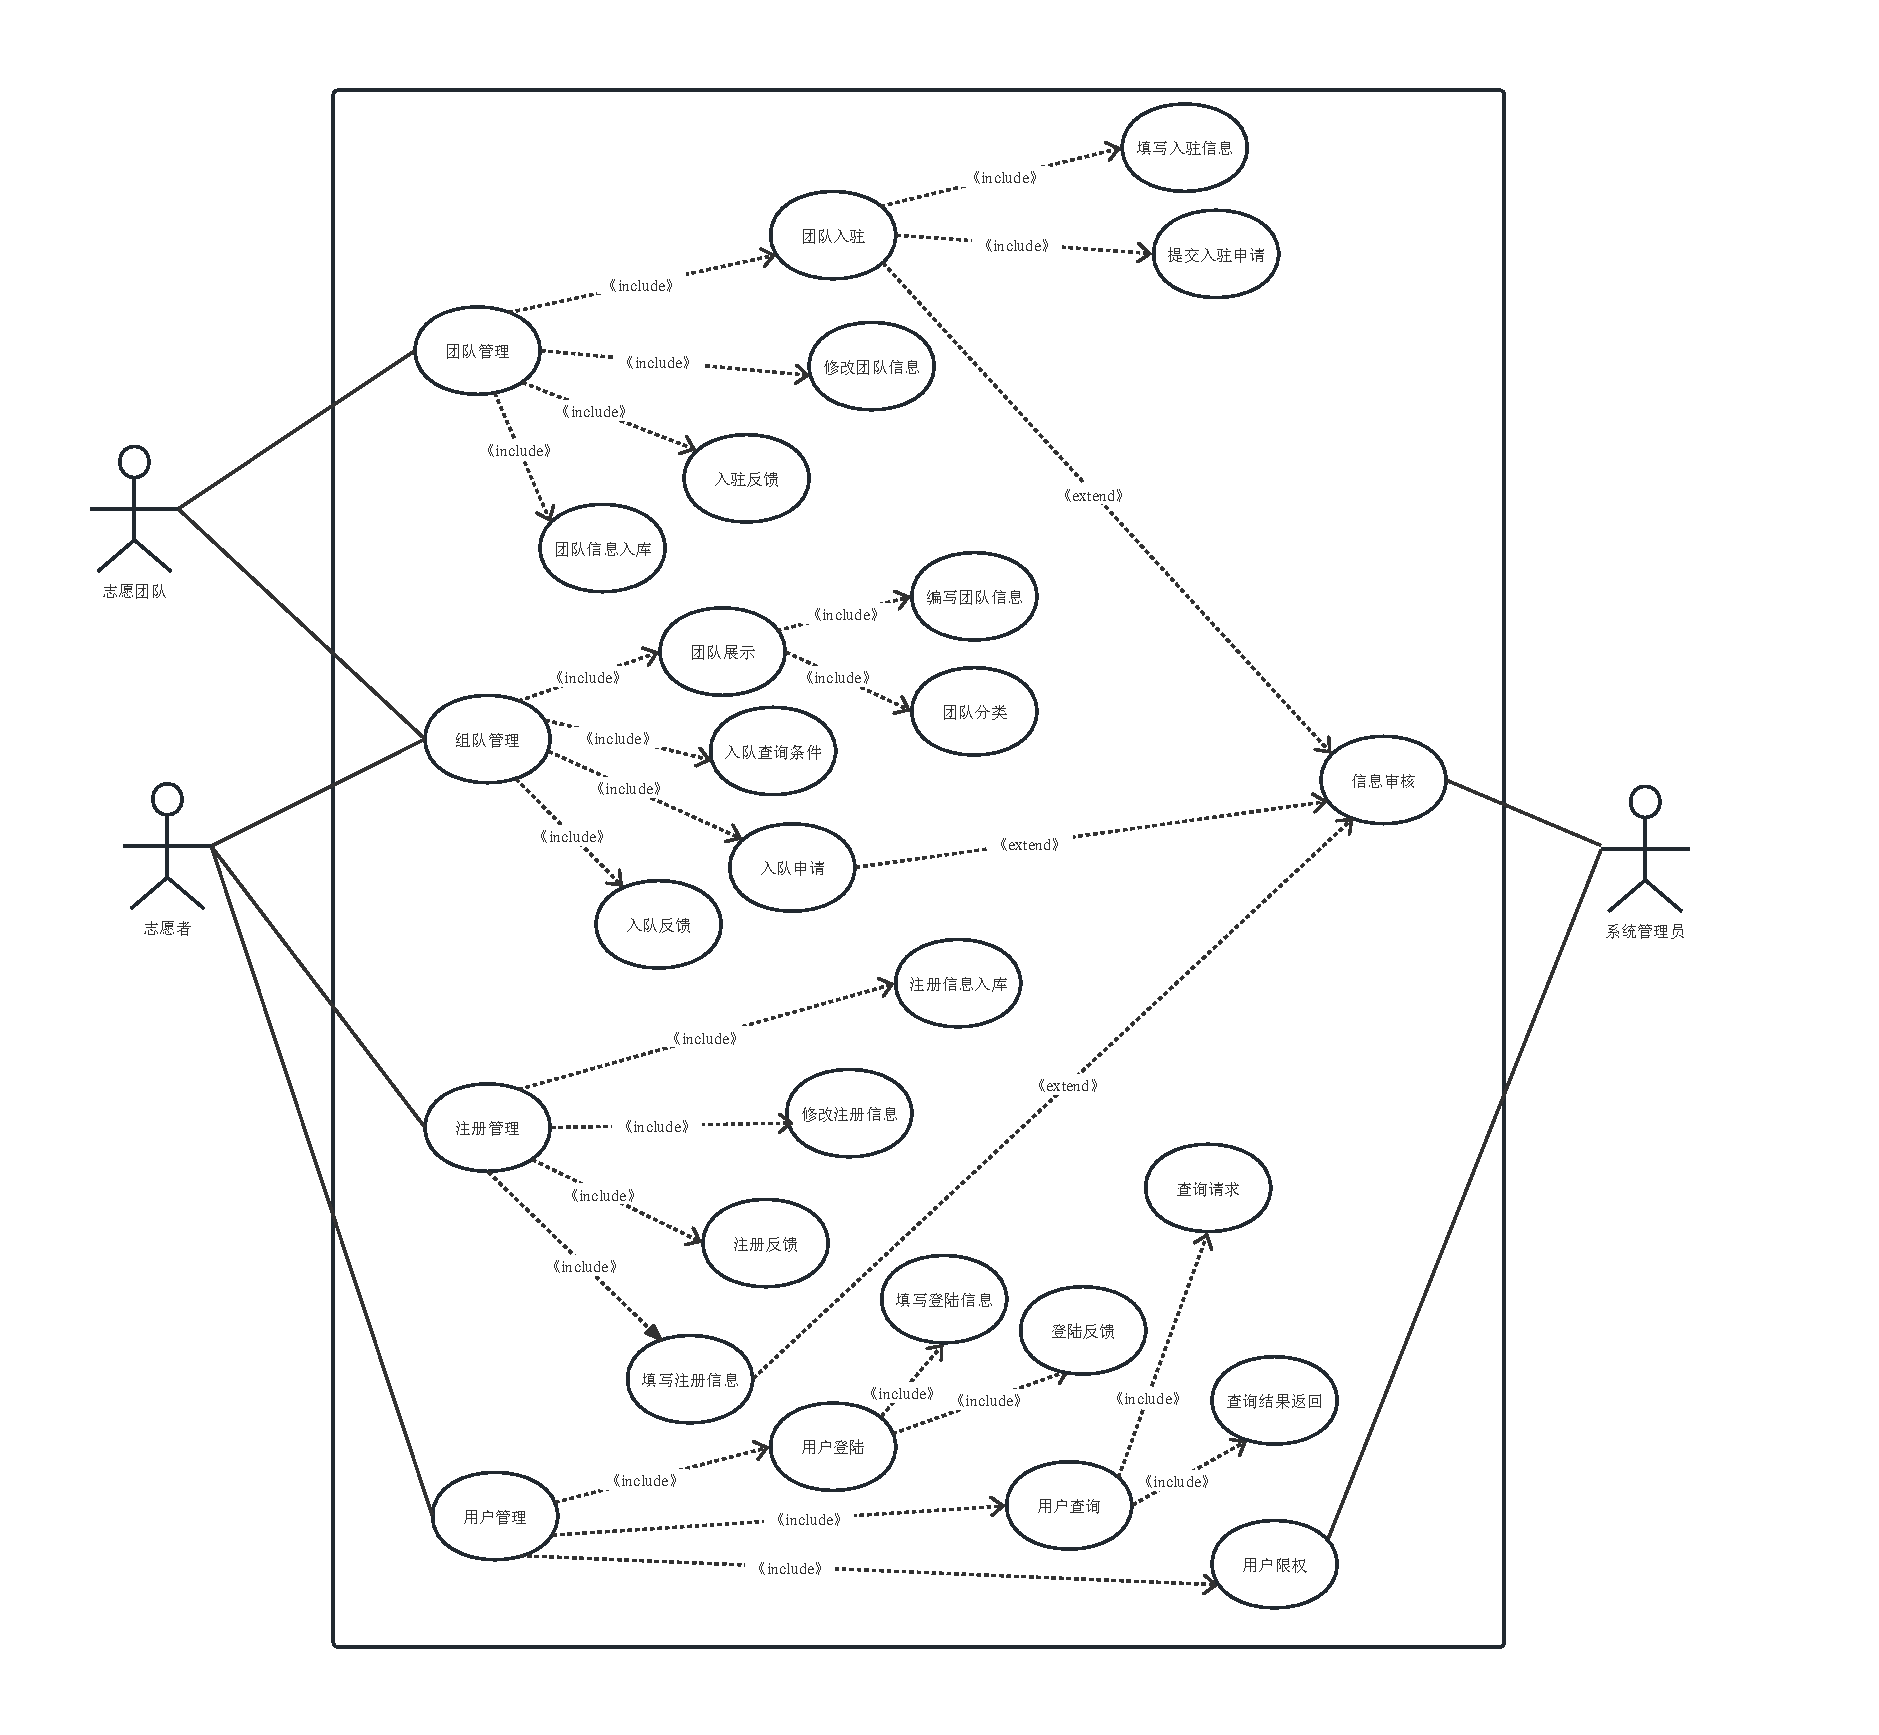
\includegraphics[scale=0.5]{OOA/fig/1-信息管理/信息管理用况图.pdf}} 
    \bicaption{Volunet信息管理系统用况图}{Information Management System Usage Chart of Volunet} 
\end{figure}


\subsubsection{志愿服务系统}
\begin{figure}[H] 
    \center{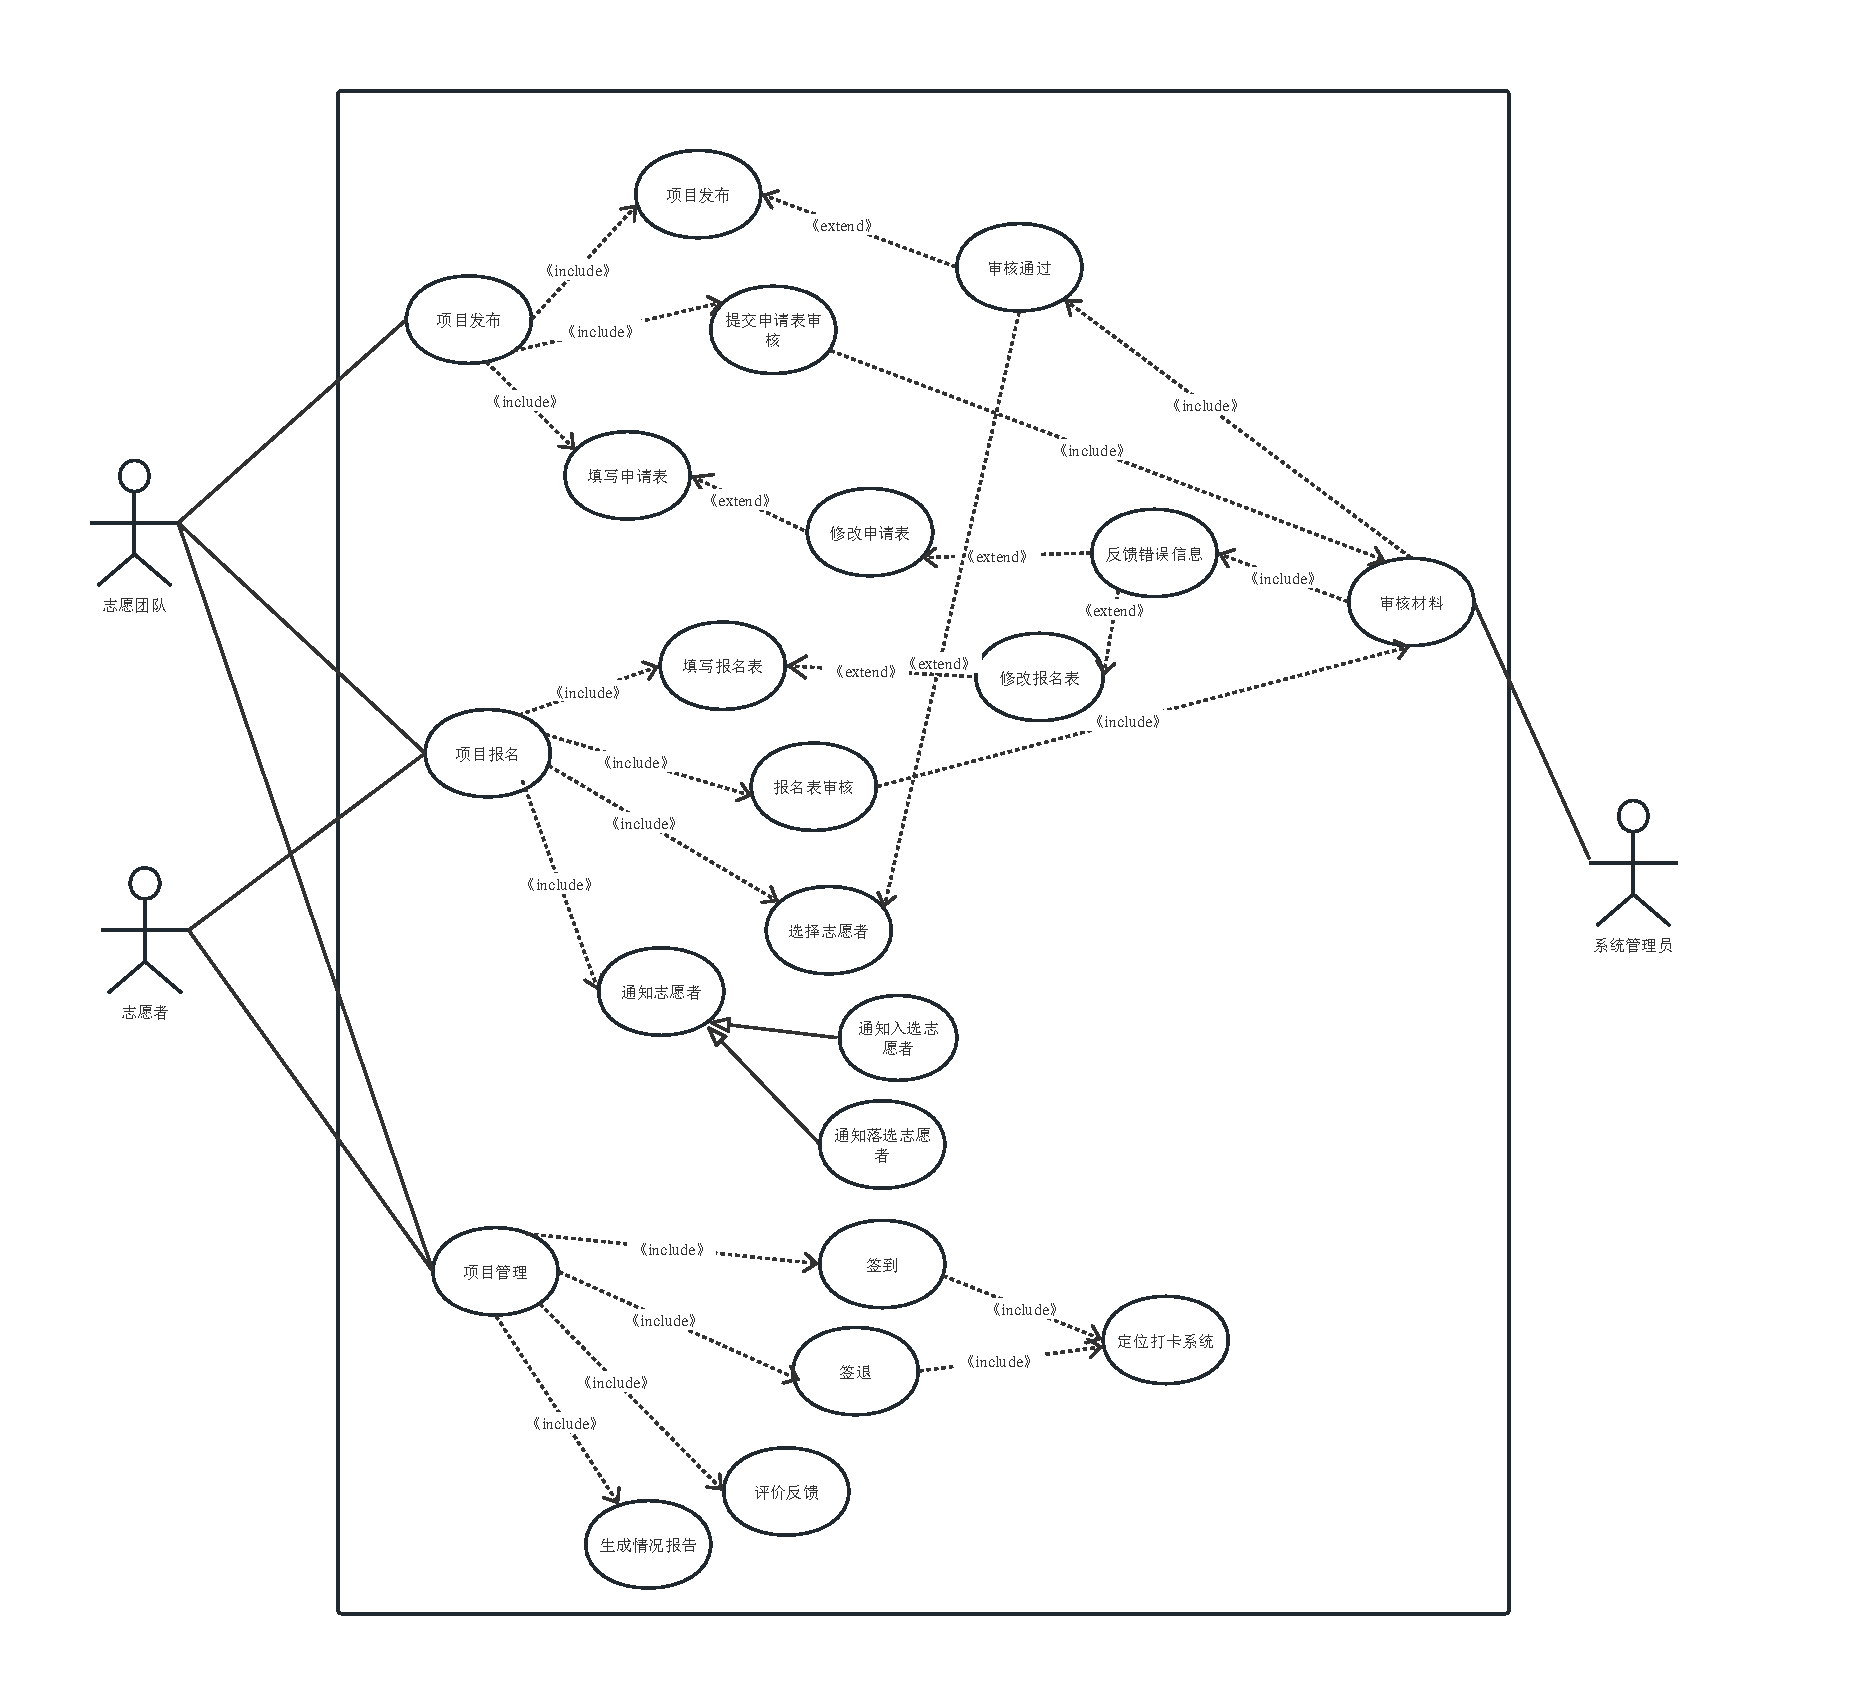
\includegraphics[scale=0.5]{OOA/fig/2-志愿服务/VS-用况图.pdf}} 
    \bicaption{Volunet志愿服务系统用况图}{Voluntary Service System Usage Chart of Volunet} 
\end{figure}


\subsubsection{爱心捐助系统}
\begin{figure}[H] 

    \center{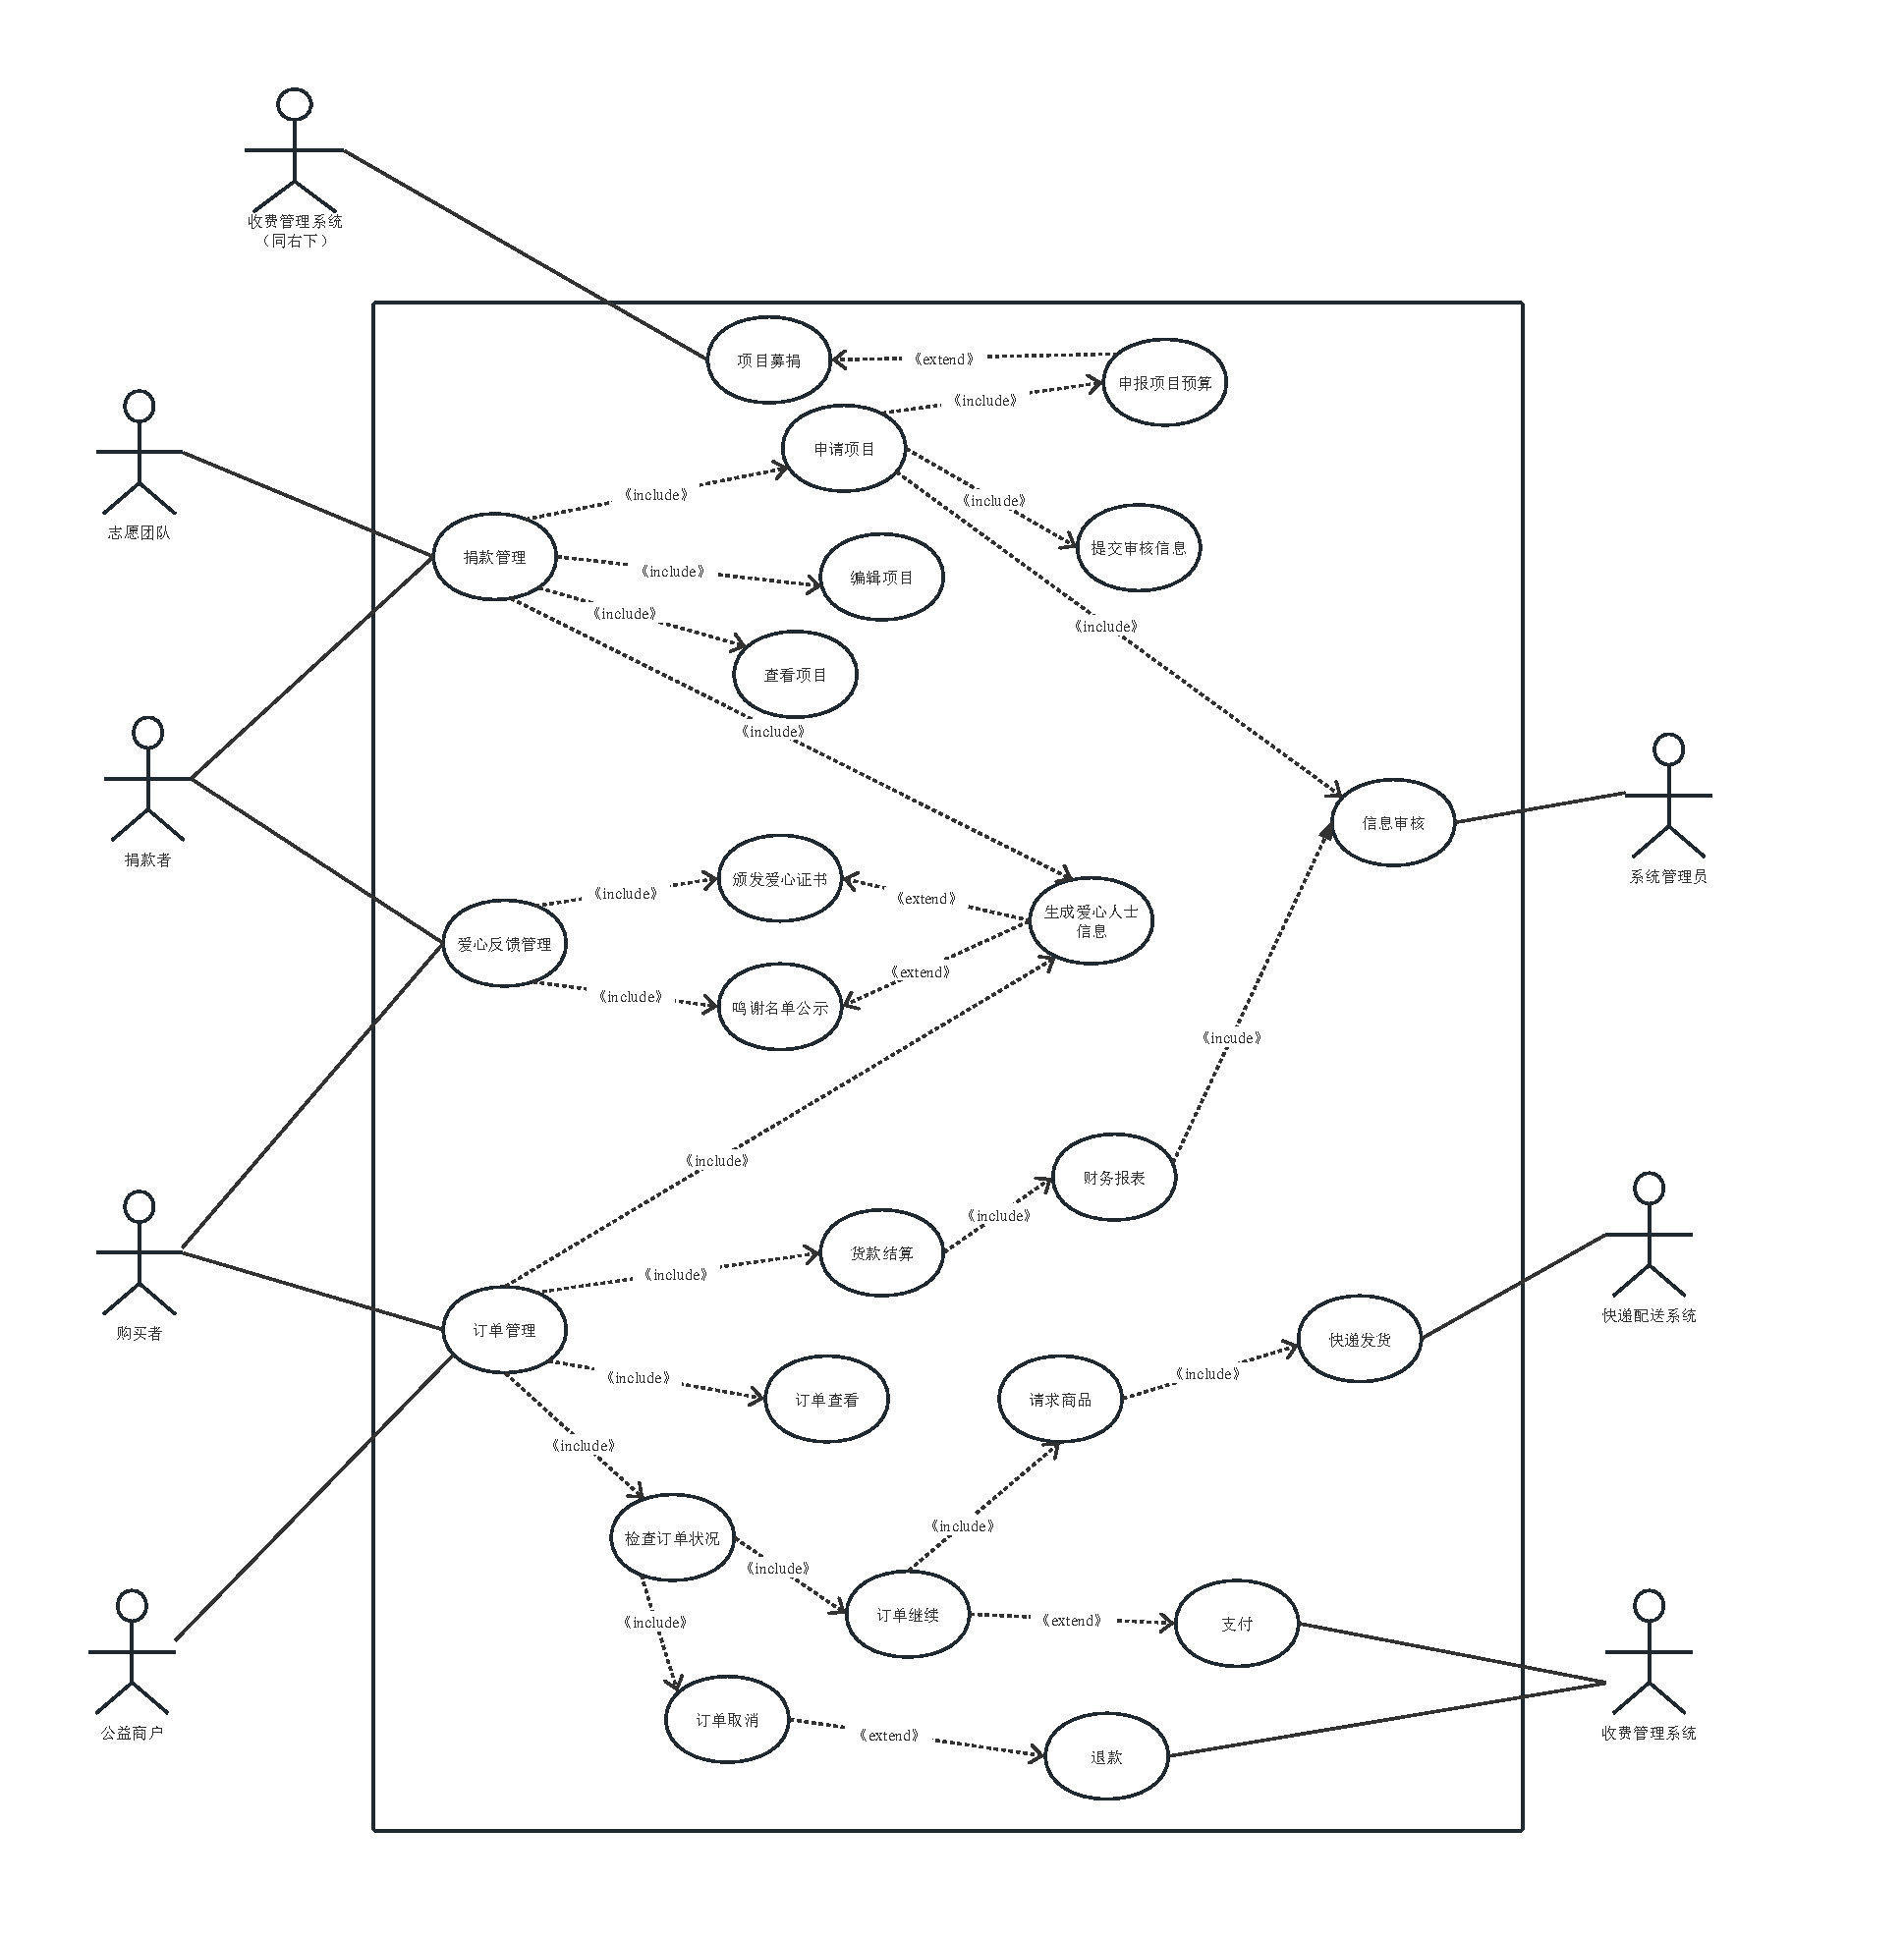
\includegraphics[scale=0.5]{OOA/fig/3-爱心管理/爱心管理用况图.pdf}} 
    \bicaption{Volunet爱心捐助系统用况图}{Love Donation System Usage Chart of Volunet} 
\end{figure}

\subsubsection{公益课程系统}
\begin{figure}[H] 

    \center{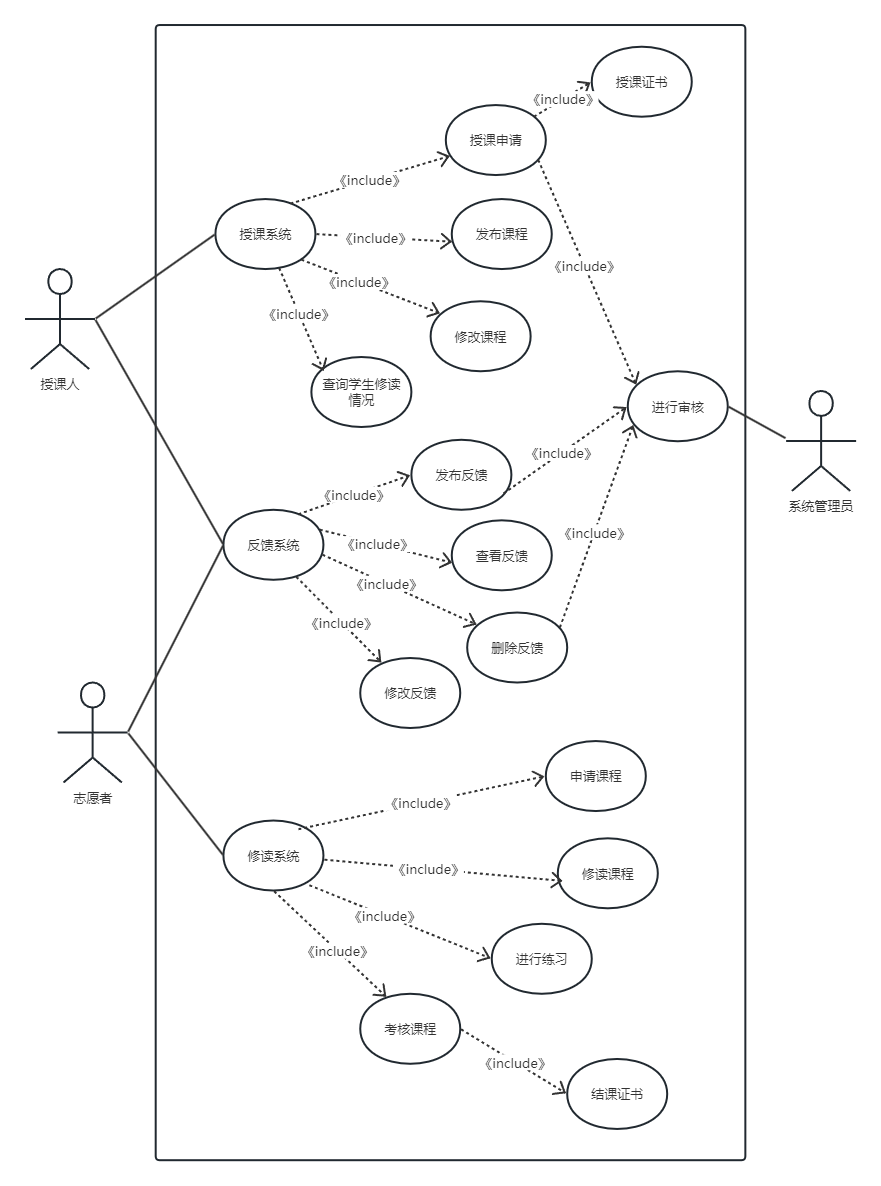
\includegraphics[scale=0.42]{OOA/fig/4-课程管理/课程管理用况图.png}} 
    \bicaption{Volunet公益课程系统用况图}{Course System Usage Chart of Volunet} 
\end{figure}

\subsubsection{交流论坛系统}
\begin{figure}[H] 

    \center{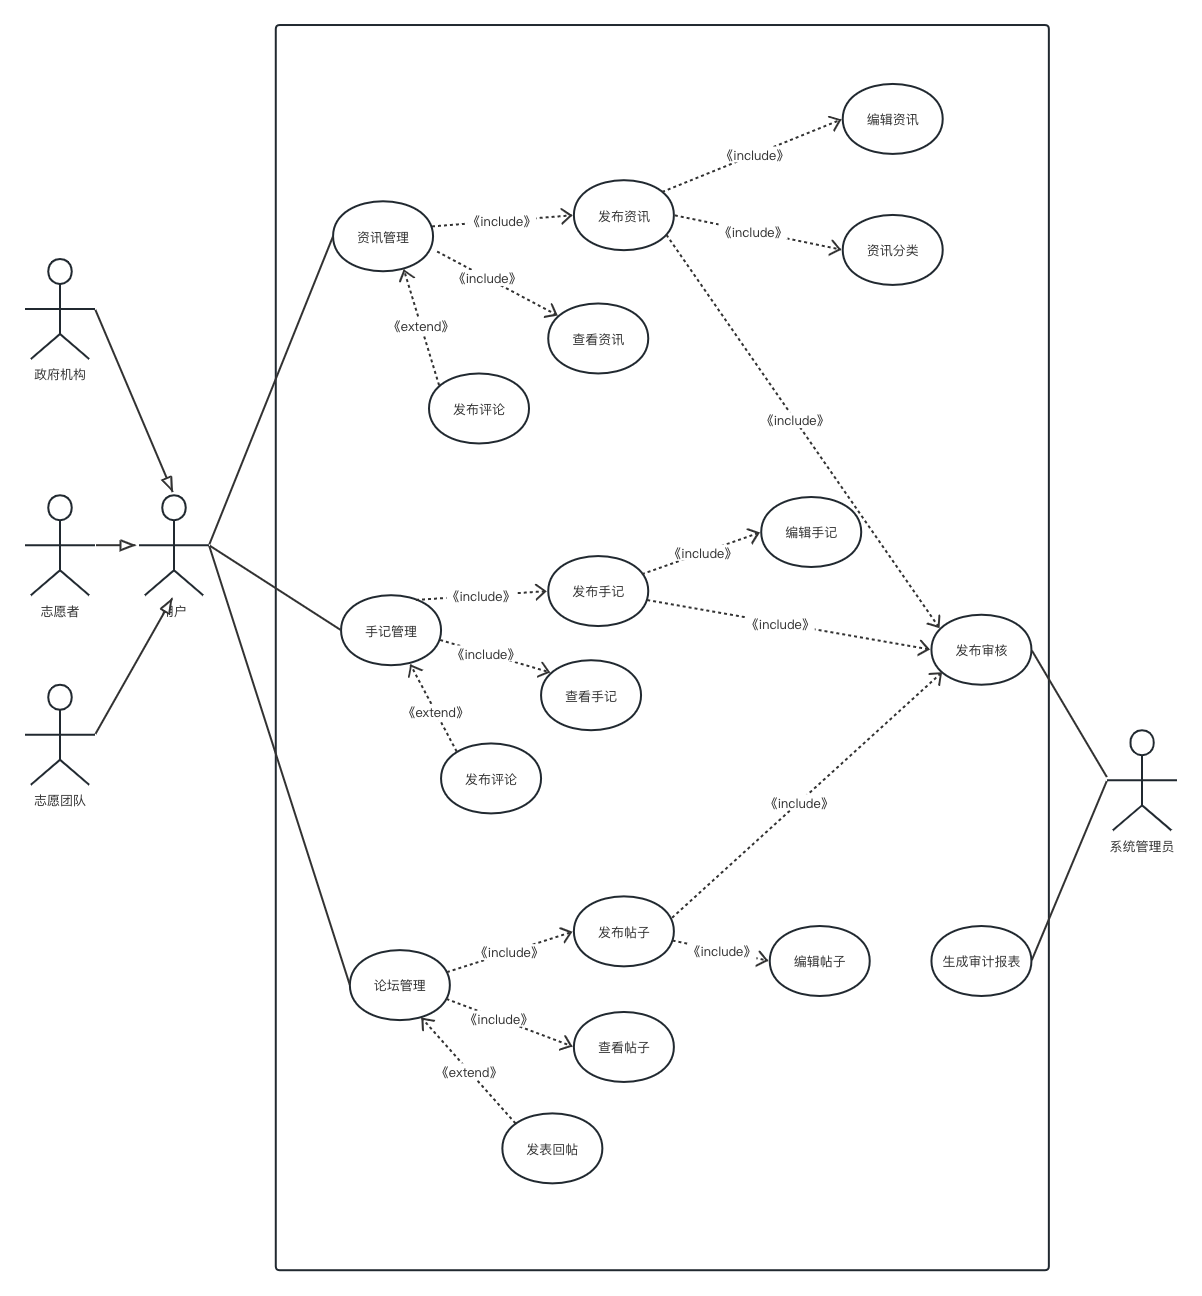
\includegraphics[scale=0.35]{OOA/fig/5-论坛管理/论坛管理用况图.png}} 
    \bicaption{Volunet交流论坛系统用况图}{Communication System Use Case Chart of Volunet} 
\end{figure}

\subsubsection{志愿交友系统}
\begin{figure}[H] 

    \center{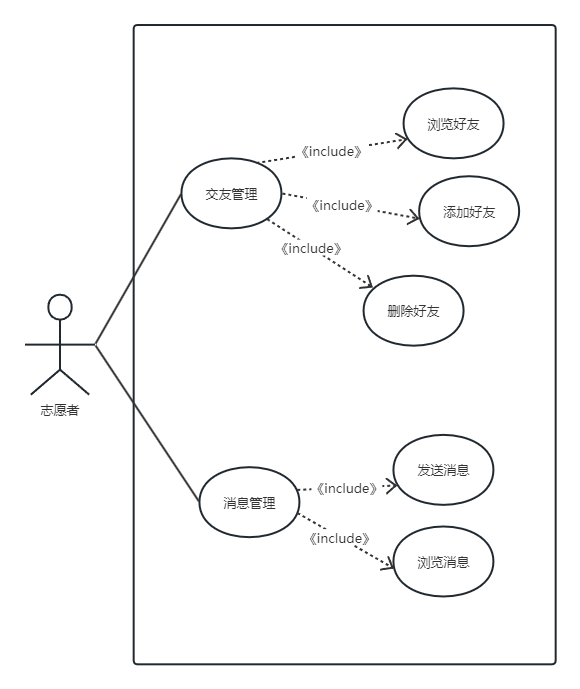
\includegraphics[scale=0.5]{OOA/fig/6-交友管理/志愿交友管理用况图.png}} 
    \bicaption{Volunet志愿交友用况图}{Volunteer Friends System Usage Chart of Volunet} 
\end{figure}

\subsection{用况描述}

\subsubsection{信息管理系统}

信息管理系统的用况描述如下:

\begin{framed}
\noindent
用况名称:用户管理\\
参与的执行者:志愿者、系统管理员\\
前置条件:用户身份为志愿者,且已经合法登陆到这个系统\\
事件流:\\
基本路径:
\begin{enumerate}[itemsep=2pt,topsep=0pt,parsep=0pt,itemindent=1em]
    \item 当志愿者进入到用户页面时,用况开始
    \item 志愿团队进行页面选择并发出操作指令
    \item 系统对志愿者的操作进行处理:
    \begin{enumerate}[itemsep=2pt,topsep=0pt,parsep=0pt,itemindent=1em]
          \item 用户主页编辑:若有权限则继续执行;否则退回到上一步
          \item 用户查找:继续执行第8步
      \end{enumerate}
    \item 志愿者进入主页编写界面
    \item 志愿者获取展示列表
    \item 志愿者按需编辑主页标题、图片和展示列表
    \item 志愿者编辑完成可预览用户主页,点击确认后提示用户主页成功更新,用况结束
    \item 志愿者浏览用户主页列表
    \item 志愿者选择搜索框并按条件查询
    \item 展示志愿者查询结果,用况结束
\end{enumerate}
\noindent
可选路径:\par
    在选择提交主页编辑之前的任何时间,志愿团队可以退出该系统,系统会自动保存当前历史记录,并在下一次进入系统时询问是否恢复\\
后置条件:用户编辑好后的主页会进行更新,替代之前的信息
\end{framed}

\begin{framed}
\noindent
用况名称:注册管理\\
参与的执行者:志愿者、系统管理员\\
前置条件:志愿者需要访问注册页面,系统管理员需要具有管理注册信息的权限,二者均已合法登陆到这个系统\\
事件流:\\
基本路径:
\begin{enumerate}[itemsep=2pt,topsep=0pt,parsep=0pt,itemindent=1em]
   \item 志愿者填写必要的信息,如用户名、密码、电子邮件地址等\item 志愿者点击“注册”按钮
   \item 系统管理员验证用户提供的信息是否有效
   \item 如果验证通过,系统将用户的信息保存到数据库中,并向志愿者发送确认邮件
   \item 志愿者收到确认邮件并点击其中的链接以激活账户 
   \item 志愿者账户激活成功,志愿者可以登录系统
\end{enumerate}
\noindent
可选路径:\par
     \begin{enumerate}[itemsep=2pt,topsep=0pt,parsep=0pt,itemindent=1em] \item 如果用户提供的信息无效,系统将显示错误消息并要求用户更正
     \item 如果用户没有收到确认邮件,用户可以请求系统重新发送 
     \end{enumerate} 
后置条件:用户账户已成功注册并激活,用户可以登录系统
\end{framed}

\begin{framed}
\noindent
用况名称:组队管理\\
参与的执行者:志愿者、志愿团队、系统管理员\\
前置条件:志愿者已经注册并登录到系统中;志愿团队已经创建并发布了一个活动\\
事件流:\\
基本路径: \begin{enumerate}[itemsep=2pt,topsep=0pt,parsep=0pt,itemindent=1em] \item 志愿者在系统中查看到志愿团队发布的活动,并决定加入该活动的团队 \item 志愿者向志愿团队发送加入请求 \item 志愿团队收到请求后,审核志愿者的信息并决定是否接受该志愿者 \item 如果志愿团队接受了志愿者的请求,系统将志愿者加入该团队,并将该团队的信息显示在志愿者的个人主页上 \end{enumerate}
\noindent
可选路径:\par
     如果志愿团队拒绝了志愿者的请求,系统将不会将志愿者加入该团队,并给志愿者发送拒绝信息 \\
后置条件:志愿者已经加入了志愿团队,并可以参加该团队发布的活动

\end{framed}

\begin{framed}
\noindent
用况名称:团队管理\\
参与的执行者:志愿团队、系统管理员\\
前置条件:志愿团队已经注册并登录到系统中,且系统管理员已经授权志愿团队进行团队管理\\
事件流:\\
基本路径:
\begin{enumerate}[itemsep=2pt,topsep=0pt,parsep=0pt,itemindent=1em] \item 志愿团队登录到系统中 \item 在系统中选择团队管理功能。 \item 在团队管理页面中,可以进行以下操作: \begin{enumerate}[itemsep=2pt,topsep=0pt,parsep=0pt,itemindent=1em] \item 添加或删除团队成员 \item 分配任务给团队成员。 \item 查看团队成员的任务进度 \item 编辑团队成员的个人信息 \item 禁止或允许团队成员访问系统\end{enumerate} 
\end{enumerate}
\noindent
可选路径: \par
 \begin{enumerate}[itemsep=2pt,topsep=0pt,parsep=0pt,itemindent=1em]  \item 在团队管理页面中,如果志愿团队没有权限进行某些操作,系统会提示“权限不足”的错误信息 \item 如果团队成员的个人信息不完整或错误,系统管理员可以要求团队成员进行修改  \end{enumerate} 
后置条件:团队成员的任务分配和进度记录已经更新到系统中;团队成员的个人信息已经保存到系统中

\end{framed}

\begin{framed}
\noindent
用况名称:信息审核\\
参与的执行者:系统管理员\\
前置条件:系统中存在需要审核的信息,且系统管理员已经合法登陆到这个系统
事件流: \begin{enumerate}[itemsep=2pt,topsep=0pt,parsep=0pt,itemindent=1em] \item 系统管理员登录审核系统 \item 系统管理员选择需要审核的信息 \item 系统管理员查看信息内容,判断是否符合审核标准 \item 如果信息符合审核标准,系统管理员将信息标记为“审核通过”,并记录审核结果 \item 如果信息不符合审核标准,系统管理员将信息标记为“审核不通过”,并记录审核结果 \end{enumerate}
\noindent
可选路径: \par
在步骤3中,如果系统管理员无法判断信息是否符合审核标准,可以将信息标记为“待定”,并将信息转交给其他审核人员审核\\
后置条件:审核结果被记录在系统中,审核完成

\end{framed}

\subsubsection{志愿服务系统}
志愿服务系统的用况描述如下:
\begin{framed}
\noindent
用况名称:项目发布\\
参与的执行者:志愿团队、系统管理员\\
前置条件:用户身份为志愿团队,且通过资质审核可以提交志愿项目发布申请\\
事件流:\\
基本路径:
\begin{enumerate}[itemsep=2pt,topsep=0pt,parsep=0pt,itemindent=1em]
    \item 当志愿团队新建志愿项目单时,用况开始
    \item 志愿团队填写志愿项目信息
    \item 志愿团队提交志愿项目申请单
    \item 系统管理员对提交的志愿项目进行审核:
    \begin{enumerate}[itemsep=2pt,topsep=0pt,parsep=0pt,itemindent=1em]
          \item 审核通过:项目发布,用况结束
          \item 审核失败:将错误信息反馈给志愿团队,转到2继续
      \end{enumerate}
\end{enumerate}
\noindent
可选路径:\par
    在选择提交志愿项目申请单之前的任何时间,志愿团队可以退出该系统,系统会自动保存当前历史记录,并在下一次进入系统时询问是否恢复\\
后置条件:项目通过审核并发布在Volunet,该项目会被编号进入志愿项目库

\end{framed}

\begin{framed} \noindent 用况名称:项目报名\\ 
参与的执行者:志愿者、志愿团队、系统管理员\\
前置条件:志愿者已经注册并登录系统\\ 
事件流:\\
基本路径: \begin{enumerate}[itemsep=2pt,topsep=0pt,parsep=0pt,itemindent=1em] \item 志愿者进入项目报名页面。 \item 系统显示可报名的项目列表。 \item 志愿者选择感兴趣的项目。 \item 系统显示该项目的详细信息和报名表格。 \item 志愿者填写报名表格并提交。 \item 系统保存志愿者的报名信息,并将其加入该项目的报名名单中。 \item 系统向志愿者发送报名成功的通知。 \end{enumerate} \noindent 
可选路径: \par
如果该项目已经满员,系统提示志愿者该项目已经无法报名,返回步骤2。如果志愿者填写的报名表格信息不完整或不符合要求,系统提示志愿者修改并重新提交,返回步骤4。 \\
 \end{framed}

 \begin{framed} \noindent 
用况名称:项目管理\\ 
参与的执行者:志愿者、志愿团队、系统管理员\\
 前置条件:项目需求已经明确并且项目计划已经制定\\
 事件流: \\
基本路径: \begin{enumerate}[itemsep=2pt,topsep=0pt,parsep=0pt,itemindent=1em] \item 系统管理员创建项目。 \item 系统管理员指派志愿者和志愿团队成员。 \item 志愿者和志愿团队成员接受任务并开始执行。 \item 志愿者和志愿团队成员定期向系统管理员报告项目进展情况。 \item 系统管理员根据报告情况对项目进度进行监控和管理。 \item 当项目完成时,系统管理员关闭项目并将成果提交给相关方。 \end{enumerate} 
可选路径: \par 
如果项目进展不如预期,系统管理员可以采取措施来加速项目进度。如果项目需求发生变化,系统管理员可以更新项目计划并通知相关人员\\
\end{framed}




\subsubsection{爱心捐助系统}

爱心捐助系统的用况描述如下:

\begin{framed}
\noindent
用况名称:捐款管理\\
参与的执行者:捐款者、志愿团队、系统管理员\\
前置条件:用户身份为志愿团队,且通过资质审核可以提交志愿项目发布申请;用户身份为捐款者,且已经合法登陆到这个系统\\
事件流:\\
基本路径:
\begin{enumerate}[itemsep=2pt,topsep=0pt,parsep=0pt,itemindent=1em]
    \item 当志愿团队新建资助项目单时,用况开始
    \item 志愿团队填写资助项目信息
    \item 志愿团队提交资助项目申请单
    \item 系统管理员对提交的信息进行审核:
    \begin{enumerate}[itemsep=2pt,topsep=0pt,parsep=0pt,itemindent=1em]
          \item 审核通过:项目发布,志愿团队相关用况结束
          \item 审核失败:将错误信息反馈给志愿团队,转到2继续
      \end{enumerate}
    \item 当捐款者选择募捐项目时,用况开始
    \item 捐款者为选择的项目输入捐款的数额
    \item 捐款者选择支付方式并进行支付
    \item 系统检验支付是否成功,如果捐款者账户的余额不足以支付,系统将提示用户支付失败并重新尝试
    \item 当支付成功后,捐款就被标记上已经支付,同时记录捐款者信息用于爱心反馈,捐款者相关用况结束
\end{enumerate}
\noindent
可选路径:\par
     \begin{enumerate}[itemsep=2pt,topsep=0pt,parsep=0pt,itemindent=1em]  \item 在选择提交资助项目申请单之前的任何时间,志愿团队可以退出该系统,系统会自动保存当前历史记录,并在下一次进入系统时询问是否恢复 \item 在支付开始之前的任何时间,捐款者可以退出该系统,系统会自动保存当前历史记录,并在下一次进入系统时询问是否恢复  \end{enumerate} 
后置条件:资助项目通过审核并添加进募捐项目列表,捐款者支付成功后的信息会保存在系统中并做标记
\end{framed}

\begin{framed}
\noindent
用况名称:订单管理\\
参与的执行者:购买者、爱心商户、系统管理员\\
前置条件:用户身份为爱心商户,且营业状态正常;用户身份为购买者,且已经合法登陆到这个系统\\
事件流:\\
基本路径:
\begin{enumerate}[itemsep=2pt,topsep=0pt,parsep=0pt,itemindent=1em]
    \item 当公益商户添加公益商品时,用况开始
    \item 公益商户填写公益商品信息
    \item 公益商户提交公益商品上架单
    \item 系统管理员对提交的商品信息进行审核:
    \begin{enumerate}[itemsep=2pt,topsep=0pt,parsep=0pt,itemindent=1em]
          \item 审核通过:商品发布,公益商户相关用况结束
          \item 审核失败:将失败信息反馈给公益商户,转到2继续
      \end{enumerate}
    \item 当购买者选择公益商品时,用况开始
    \item 购买者将选择的公益商品加入购物车并提交订单
    \item 购买者选择支付方式并进行支付
    \item 系统检验支付是否成功,如果捐款者账户的余额不足以支付,系统将提示用户支付失败并重新尝试
    \item 当支付成功后,订单就被标记上已经支付
    \item 支付完成的订单将接入快递配送平台进行配送
    \item 购买者收到货物后对订单进行签收
    \item 订单完结,同时记录购买者信息用于爱心反馈,购买者相关用况结束
\end{enumerate}
\noindent
可选路径:\par
         \begin{enumerate}[itemsep=2pt,topsep=0pt,parsep=0pt,itemindent=1em]  \item 在选择提交公益商品信息之前的任何时间,公益商户可以退出该系统,系统会自动保存当前历史记录,并在下一次进入系统时询问是否恢复 \item 在用况开始到支付开始之前以及支付完成之后的任何时间,购买者可以退出该系统,系统会自动保存当前历史记录,并在下一次进入系统时询问是否恢复  \end{enumerate} 
后置条件:公益商品通过审核并添加进商品页面,购买者订单完成后的信息会保存在系统中并做标记
\end{framed}

\begin{framed}
\noindent
用况名称:爱心反馈管理\\
参与的执行者:捐款者、购买者\\
前置条件:用户身份为爱心人士(即捐款者和购买者),且已经合法登陆到这个系统\\
事件流:\\
基本路径:
\begin{enumerate}[itemsep=2pt,topsep=0pt,parsep=0pt,itemindent=1em]
    \item 当爱心人士查看爱心反馈页面时,用况开始
    \item 爱心人士选择查看内容:
    \begin{enumerate}[itemsep=2pt,topsep=0pt,parsep=0pt,itemindent=1em]
          \item 查看爱心证书:显示其对应的爱心证书,用况结束
          \item 查看鸣谢名单:显示公示的鸣谢爱心人士名单,用况结束
      \end{enumerate}
\end{enumerate}
\noindent
可选路径:\par
    在任何时间,爱心人士可以退出该系统,系统会自动保存当前历史记录,并在下一次进入系统时询问是否恢复\\
后置条件:无

\end{framed}

\begin{framed}
\noindent
用况名称:信息审核\\
参与的执行者:系统管理员\\
前置条件:系统中存在需要审核的信息,且系统管理员已经合法登陆到这个系统
事件流: \begin{enumerate}[itemsep=2pt,topsep=0pt,parsep=0pt,itemindent=1em] \item 系统管理员登录审核系统 \item 系统管理员选择需要审核的信息 \item 系统管理员查看信息内容,判断是否符合审核标准 \item 如果信息符合审核标准,系统管理员将信息标记为“审核通过”,并记录审核结果 \item 如果信息不符合审核标准,系统管理员将信息标记为“审核不通过”,并记录审核结果 \end{enumerate}
\noindent
可选路径: \par
在步骤3中,如果系统管理员无法判断信息是否符合审核标准,可以将信息标记为“待定”,并将信息转交给其他审核人员审核\\
后置条件:审核结果被记录在系统中,审核完成

\end{framed}

\subsubsection{公益课程系统}

公益课程系统的用况描述如下:

\begin{framed}
\noindent
用况名称:授课管理\\
参与的执行者:授课人、系统管理员\\
前置条件:用户身份为状态无异常账号,且通过资质审核可以提交课程项目发布申请;用户身份为系统管理员,且已经合法登陆到这个系统\\
事件流:\\
基本路径:
\begin{enumerate}[itemsep=2pt,topsep=0pt,parsep=0pt,itemindent=1em]
    \item 当用户新创建授课申请单时,用况开始
    \item 用户填写授课申请单信息
    \item 用户提交授课申请单
    \item 系统管理员对提交的信息进行审核:
    \begin{enumerate}[itemsep=2pt,topsep=0pt,parsep=0pt,itemindent=1em]
          \item 审核通过:资质核验通过发布,用户获得授课资格,成为授课人
          \item 审核失败:将核验信息反馈给授课人,转到2继续
      \end{enumerate}
    \item 当授课人选择创建课程时,用况开始
    \item 授课人为创建的课程输入必要的信息
    \item 授课人选择为创建的课程导入必要的课程资料
    \item 授课进行发布课程,在课程首页可以获得展示
\end{enumerate}
\noindent
可选路径:\par
     \begin{enumerate}[itemsep=2pt,topsep=0pt,parsep=0pt,itemindent=1em]  \item 系统管理员将授课人分配到不同的课程中,进行管理和监督教学工作。 \item 授课人创建考试和评估任务,对学生进行考核和评估。  \end{enumerate} 
后置条件:授课人完成课程的上课记录,系统需要自动计算学生的考勤情况并更新到学生的考勤记录中
\end{framed}

\begin{framed}
\noindent
用况名称:修读管理\\
参与的执行者:授课人、志愿者、系统管理员\\
前置条件:用户身份为授课人,且资质状态正常;用户身份为志愿者,且已经合法登陆到这个系统\\
事件流:\\
基本路径:
\begin{enumerate}[itemsep=2pt,topsep=0pt,parsep=0pt,itemindent=1em]
    \item 当志愿者选择查看课程时,用况开始
    \item 志愿者选择查看具体课程信息
    \item 志愿者提交选课申请
    \item 系统管理员对提交的选课申请信息进行审核:
    \begin{enumerate}[itemsep=2pt,topsep=0pt,parsep=0pt,itemindent=1em]
          \item 审核通过:课程选择成功,志愿者成为此课程学生
          \item 审核失败:将失败信息反馈给志愿者,转到2继续
      \end{enumerate}
    \item 当志愿者购买课程时,用况开始
    \item 志愿者将选择的课程加入购物车并提交订单
    \item 志愿者选择支付方式并进行支付
    \item 系统检验支付是否成功,如果志愿者账户的余额不足以支付,系统将提示志愿者支付失败并重新尝试
    \item 当支付成功后,订单就被标记上已经支付
    \item 当前订单的课程向此志愿者进行解锁
    \item 志愿者可以对课程进行学习、并与授课人交流提问
    \item 课程完结,同时记录志愿者信息用于课程反馈,志愿者相关用况结束
\end{enumerate}
\noindent
可选路径:\par
         \begin{enumerate}[itemsep=2pt,topsep=0pt,parsep=0pt,itemindent=1em]  \item 在选择提交课程之前的任何时间,志愿者可以退出该系统,系统会自动保存当前历史记录,并在下一次进入系统时询问是否恢复 
         \item 在用况开始到支付开始之前以及支付完成之后的任何时间,志愿者可以退出该系统,系统会自动保存当前历史记录,并在下一次进入系统时询问是否恢复  \end{enumerate} 
后置条件:完成一定的课程和通过相关考试后,提供相关结课证书
\end{framed}

\begin{framed}
\noindent
用况名称:反馈管理\\
参与的执行者:志愿者、系统管理员、授课人\\
前置条件:用户身份为志愿者、系统管理员或授课人,且已经合法登陆到这个系统\\
事件流:\\
基本路径:
\begin{enumerate}[itemsep=2pt,topsep=0pt,parsep=0pt,itemindent=1em]
    \item 当志愿者选择课程反馈界面时,用况开始
    \item 志愿者选择撰写课程反馈界面
    \item 志愿者提交课程反馈
    \item 系统管理员对提交的反馈信息进行审核:
    \begin{enumerate}[itemsep=2pt,topsep=0pt,parsep=0pt,itemindent=1em]
          \item 审核通过:课程反馈发布成功,志愿者用况结束
          \item 审核失败:将审核失败信息反馈给志愿者,转到2继续
      \end{enumerate}
    \item 当授课人查看课程反馈页面时,用况开始
    \item 授课人选择查看内容:
    \begin{enumerate}[itemsep=2pt,topsep=0pt,parsep=0pt,itemindent=1em]
          \item 查看学生修读情况:显示其对应的修读情况,用况结束
          \item 查看课程反馈:显示提交的课程反馈,用况结束
      \end{enumerate}
\end{enumerate}
\noindent
可选路径:\par
         \begin{enumerate}[itemsep=2pt,topsep=0pt,parsep=0pt,itemindent=1em]  \item 在任何时间,用户可以退出该系统,系统会自动保存当前历史记录,并在下一次进入系统时询问是否恢复 
         \item 如果系统管理员无法判断反馈信息是否符合审核标准,可以将信息标记为“待定”,并将信息转交给其他审核人员审核  \end{enumerate}
后置条件:反馈结果被记录在系统中,反馈完成

\end{framed}


\subsubsection{交流论坛系统}

交流论坛系统的用况描述如下:
\begin{framed}
\noindent
用况名称:资讯管理\\
参与的执行者:用户\\
前置条件:一个合法的用户已经登录到了这个系统\\
事件流:\\
基本路径:
\begin{enumerate}[itemsep=2pt,topsep=0pt,parsep=0pt,itemindent=1em]
    \item 用户通过身份验证进入资讯管理系统,用况开始
    \item 用户点击“资讯管理”按钮
    \item 进入资讯管理主界面
    \item 显示资讯目录
    \item 当用户点击查看资讯时以任意次数和合理的次序重复如下事件流,直至出现创建资讯事件流
    \begin{enumerate}[itemsep=2pt,topsep=0pt,parsep=0pt,itemindent=1em]
          \item 系统展示资讯
          \item 用户评论资讯
      \end{enumerate}
    \item 用户选择发布资讯
    \item 以任意次数和合理的次序重复如下事件流,直至出现发布事件流
    \begin{enumerate}[itemsep=2pt,topsep=0pt,parsep=0pt,itemindent=1em]
          \item 编辑资讯
          \item 资讯分类
          \item 发布审核
      \end{enumerate}
    \item 发布资讯或退出
        \begin{enumerate}[itemsep=2pt,topsep=0pt,parsep=0pt,itemindent=1em]
          \item 发布资讯
          \item 退出资讯管理
      \end{enumerate}
\end{enumerate}
\noindent
可选路径:\par
   \begin{enumerate}[itemsep=2pt,topsep=0pt,parsep=0pt,itemindent=1em]  \item 在选择发布资讯前的任何时候,用户都可以退出系统,待发布的资讯作为草稿保存 \item 在基本路径的第$5$步,如果有任何不合法的信息,系统提示用户去修改这些信息\item 在基本路径的第$7$步,如果有任何不合法的信息,系统提示用户去修改这些信息  \end{enumerate} 
后置条件:如果用户提交成功,资讯管理系统会执行相关操作;否则,维持不变
\end{framed}

\begin{framed}
\noindent
用况名称:发布资讯\\
参与的执行者:用户\\
前置条件:成功登录到资讯管理主页面\\
事件流:\\
基本路径:
\begin{enumerate}[itemsep=2pt,topsep=0pt,parsep=0pt,itemindent=1em]
     \item 选择待发布的资讯
     \item 发布资讯
\end{enumerate}
\noindent
后置条件:资讯
\end{framed}


\begin{framed}
\noindent
用况名称:编辑资讯\\
参与的执行者:用户\\
前置条件:成功登录到资讯管理主页面\\
事件流:\\
基本路径:
\begin{enumerate}[itemsep=2pt,topsep=0pt,parsep=0pt,itemindent=1em]
    \item 用户点击资讯
    \item 用户点击写资讯
    \item 转到文章编辑页面,输入标题或正文
    \begin{enumerate}[itemsep=2pt,topsep=0pt,parsep=0pt,itemindent=1em]
          \item 发布刚刚编辑的资讯
          \item 存为草稿或私人文章 
      \end{enumerate}
\end{enumerate}
\noindent
后置条件:资讯
\end{framed}

\begin{framed}
\noindent
用况名称:资讯分类\\
参与的执行者:用户\\
前置条件:成功登录到资讯管理主页面\\
事件流:\\
基本路径:
\begin{enumerate}[itemsep=2pt,topsep=0pt,parsep=0pt,itemindent=1em]
    \item 用户点击资讯
    \item 用户点击写资讯
    \item 转到文章编辑页面,输入标题或正文
    \begin{enumerate}[itemsep=2pt,topsep=0pt,parsep=0pt,itemindent=1em]
          \item 发布刚刚编辑的资讯
          \item 存为草稿或私人文章 
      \end{enumerate}
\end{enumerate}
\noindent
后置条件:资讯
\end{framed}

\begin{framed}
\noindent
用况名称:查看资讯\\
参与的执行者:用户\\
前置条件:成功登录到资讯管理主页面\\
事件流:\\
基本路径:
\begin{enumerate}[itemsep=2pt,topsep=0pt,parsep=0pt,itemindent=1em]
    \item 用户点击资讯
    \item 查看所有资讯
    \begin{enumerate}[itemsep=2pt,topsep=0pt,parsep=0pt,itemindent=1em]
          \item 按资讯分类查看
          \item 按资讯归档查看
      \end{enumerate}
\end{enumerate}
\noindent
后置条件:查看之前发表过的资讯或草稿
\end{framed}

\begin{framed}
\noindent
用况名称:资讯评论\\
参与的执行者:用户\\
前置条件:成功登录到资讯管理主页面\\
事件流:\\
基本路径:
\begin{enumerate}[itemsep=2pt,topsep=0pt,parsep=0pt,itemindent=1em]
    \item 用户点击资讯
    \item 查看所有资讯
    \item 选择资讯点击评论
    \item 编辑资讯评论正文
    \item 选择提交评论
    \end{enumerate}
\noindent
后置条件:资讯评论成功
\end{framed}

\begin{framed}
\noindent
用况名称:手记管理\\
参与的执行者:用户\\
前置条件:一个合法的用户已经登录到了这个系统\\
事件流:\\
基本路径:
\begin{enumerate}[itemsep=2pt,topsep=0pt,parsep=0pt,itemindent=1em]
    \item 用户通过身份验证进入手记管理系统,用况开始
    \item 用户点击“手记管理”按钮
    \item 进入手记管理主界面
    \item 显示手记目录
    \item 当用户点击查看手记时以任意次数和合理的次序重复如下事件流,直至出现创建手记事件流
    \begin{enumerate}[itemsep=2pt,topsep=0pt,parsep=0pt,itemindent=1em]
          \item 系统展示手记
          \item 用户评论手记
      \end{enumerate}
    \item 用户选择发布手记
    \item 以任意次数和合理的次序重复如下事件流,直至出现发布事件流
    \begin{enumerate}[itemsep=2pt,topsep=0pt,parsep=0pt,itemindent=1em]
          \item 编辑手记
          \item 发布审核
      \end{enumerate}
    \item 发布手记或退出
        \begin{enumerate}[itemsep=2pt,topsep=0pt,parsep=0pt,itemindent=1em]
          \item 发布手记
          \item 退出手记管理
      \end{enumerate}
\end{enumerate}
\noindent
可选路径:\par
   \begin{enumerate}[itemsep=2pt,topsep=0pt,parsep=0pt,itemindent=1em]  \item 在选择发布手记前的任何时候,用户都可以退出系统,待发布的手记作为草稿保存 \item 在基本路径的第$5$步,如果有任何不合法的信息,系统提示用户去修改这些信息\item 在基本路径的第$7$步,如果有任何不合法的信息,系统提示用户去修改这些信息  \end{enumerate} 
后置条件:如果用户提交成功,手记管理系统会执行相关操作;否则,维持不变
\end{framed}

\begin{framed}
\noindent
用况名称:发布手记\\
参与的执行者:用户\\
前置条件:成功登录到手记管理主页面\\
事件流:\\
基本路径:
\begin{enumerate}[itemsep=2pt,topsep=0pt,parsep=0pt,itemindent=1em]
    \item 选择待发布的手记
    \item 发布手记
\end{enumerate}
\noindent
后置条件:发表编辑好的手记,或者存问草稿或私人手记
\end{framed}

\begin{framed}
\noindent
用况名称:编辑手记\\
参与的执行者:用户\\
前置条件:成功登录到资讯管理主页面\\
事件流:\\
基本路径:
\begin{enumerate}[itemsep=2pt,topsep=0pt,parsep=0pt,itemindent=1em]
    \item 用户点击资讯
    \item 用户点击写资讯
    \item 转到文章编辑页面,输入标题或正文
    \begin{enumerate}[itemsep=2pt,topsep=0pt,parsep=0pt,itemindent=1em]
          \item 发布刚刚编辑的资讯
          \item 存为草稿或私人文章 
      \end{enumerate}
\end{enumerate}
\noindent
后置条件:资讯
\end{framed}

\begin{framed}
\noindent
用况名称:查看手记\\
参与的执行者:用户\\
前置条件:成功登录到手记管理主页面\\
事件流:\\
基本路径:
\begin{enumerate}[itemsep=2pt,topsep=0pt,parsep=0pt,itemindent=1em]
    \item 用户点击手记
    \item 查看所有手记
    \begin{enumerate}[itemsep=2pt,topsep=0pt,parsep=0pt,itemindent=1em]
          \item 按手记分类查看
          \item 按手记归档查看
      \end{enumerate}
\end{enumerate}
\noindent
后置条件:查看之前发表过的手记或草稿
\end{framed}

\begin{framed}
\noindent
用况名称:手记评论\\
参与的执行者:用户\\
前置条件:成功登录到手记管理主页面\\
事件流:\\
基本路径:
\begin{enumerate}[itemsep=2pt,topsep=0pt,parsep=0pt,itemindent=1em]
    \item 用户点击手记
    \item 查看所有手记
    \item 选择手记点击评论
    \item 编辑手记评论正文
    \item 选择提交评论
    \end{enumerate}
\noindent
后置条件:手记评论成功
\end{framed}

\begin{framed}
\noindent
用况名称:论坛管理\\
参与的执行者:用户\\
前置条件:一个合法的用户已经登录到了这个系统\\
事件流:\\
基本路径:
\begin{enumerate}[itemsep=2pt,topsep=0pt,parsep=0pt,itemindent=1em]
    \item 用户通过身份验证进入论坛管理系统,用况开始
    \item 用户点击“论坛管理”按钮
    \item 进入论坛管理主界面
    \item 显示板块目录
    \item 点击进入板块
    \item 当用户点击查看资讯时以任意次数和合理的次序重复如下事件流,直至出现创建资讯事件流
    \begin{enumerate}[itemsep=2pt,topsep=0pt,parsep=0pt,itemindent=1em]
          \item 系统展示帖子
          \item 用户回帖
      \end{enumerate}
    \item 用户选择发布帖子
    \item 以任意次数和合理的次序重复如下事件流,直至出现发布事件流
    \begin{enumerate}[itemsep=2pt,topsep=0pt,parsep=0pt,itemindent=1em]
          \item 编辑帖子 
          \item 发布审核
      \end{enumerate}
    \item 发布资讯或退出
        \begin{enumerate}[itemsep=2pt,topsep=0pt,parsep=0pt,itemindent=1em]
          \item 发布帖子
          \item 退出论坛管理
      \end{enumerate}
\end{enumerate}
\noindent
可选路径:\par
   \begin{enumerate}[itemsep=2pt,topsep=0pt,parsep=0pt,itemindent=1em]  
       \item 在选择发布帖子前的任何时候,用户都可以退出系统,待发布的帖子作为草稿保存 
       \item 在基本路径的第$5$步,如果有任何不合法的信息,系统提示用户去修改这些信息
       \item 在基本路径的第$7$步,如果有任何不合法的信息,系统提示用户去修改这些信息  
   \end{enumerate} 
后置条件:如果用户提交成功,论坛管理系统会执行相关操作;否则,维持不变
\end{framed}

\begin{framed}
\noindent
用况名称:发布帖子\\
参与的执行者:用户\\
前置条件:成功登录到帖子管理主页面且用户有发帖权限\\
事件流:\\
基本路径:
\begin{enumerate}[itemsep=2pt,topsep=0pt,parsep=0pt,itemindent=1em]
    \item 用户点击创建新帖子按钮
    \item 用户编辑帖子
    \item 用户点击发布按钮
    \item 系统接收到新帖子的请求,并验证帖子的合法性
    \item 如果帖子符合论坛规则,系统将帖子添加到相应的版块,并向用户显示成功发布的信息
\end{enumerate}
\noindent
后置条件:发布成功的帖子已经在论坛上可见,其他用户可以查看并对其进行回复
\end{framed}

\begin{framed}
\noindent
用况名称:编辑帖子\\
参与的执行者:用户\\
前置条件:成功登录到帖子管理主页面且用户有发帖权限\\
事件流:\\
基本路径:
\begin{enumerate}[itemsep=2pt,topsep=0pt,parsep=0pt,itemindent=1em]
    \item 用户点击创建新帖子按钮
    \item 系统展示新帖子的编辑界面
    \item 用户输入帖子的标题和内容
\end{enumerate}
\noindent
可选路径:\par
   \begin{enumerate}[itemsep=2pt,topsep=0pt,parsep=0pt,itemindent=1em]  
       \item 用户在编辑帖子时,可以选择添加图片,链接,或其他媒体文件 
       \item 如果帖子内容不符合论坛规则,系统会拒绝发布,并向用户显示相应的错误信息
       \item 用户可以选择保存帖子草稿,稍后继续编辑和发布 
   \end{enumerate} 
后置条件:帖子进入审查阶段
\end{framed}

\begin{framed}
\noindent
用况名称:查看帖子\\
参与的执行者:用户\\
前置条件:用户已经注册并登录论坛\\
事件流:\\
基本路径:
\begin{enumerate}[itemsep=2pt,topsep=0pt,parsep=0pt,itemindent=1em]
    \item 用户浏览论坛的版块或首页,寻找感兴趣的帖子
    \item 用户点击帖子标题或预览图片
    \item 系统显示选定的帖子的全文内容,包括标题,正文,图片,回复等信息
\end{enumerate}
\noindent
可选路径:\par
   \begin{enumerate}[itemsep=2pt,topsep=0pt,parsep=0pt,itemindent=1em]  
       \item 用户可以选择将感兴趣的帖子加入收藏,或分享给其他用户或社交平台 
       \item 用户可以选择对帖子或其作者进行评分或点赞
   \end{enumerate} 
后置条件:用户已经查看了帖子的全文内容,并进行了可能的互动
\end{framed}

\begin{framed}
\noindent
用况名称:发送回帖\\
参与的执行者:用户\\
前置条件:用户已经选择了一个特定的帖子进行回复且用户有发帖和回帖的权限\\
事件流:\\
基本路径:
\begin{enumerate}[itemsep=2pt,topsep=0pt,parsep=0pt,itemindent=1em]
    \item 用户在选定的帖子下方的回复区域输入回复内容
    \item 用户点击发布回帖按钮
    \item 系统接收到回帖请求,并验证回帖内容的合法性
    \item 如果回帖符合论坛规则,系统将回帖添加到相应的帖子下,并向用户显示成功发布的信息
    \end{enumerate}
\noindent
可选路径:\par
   \begin{enumerate}[itemsep=2pt,topsep=0pt,parsep=0pt,itemindent=1em]  
       \item 用户在回帖时,可以选择引用帖子或其他回帖的内容
       \item 如果回帖内容不符合论坛规则,系统会拒绝发布,并向用户显示相应的错误信息
       \item 用户可以选择保存回帖草稿,稍后继续编辑和发布
   \end{enumerate} 
后置条件:发布成功的回帖已经在帖子下可见,其他用户可以查看并对其进行回复或点赞
\end{framed}

\begin{framed}
\noindent
用况名称:发布审核\\
参与的执行者:用户,系统管理员\\
前置条件:用户已经注册并登录系统且已经撰写了待发布信息。\\
事件流:\\
基本路径:
\begin{enumerate}[itemsep=2pt,topsep=0pt,parsep=0pt,itemindent=1em]
    \item 用户在系统中提交一篇信息。
    \item 系统接收到用户的信息后,将其发送给系统管理员进行审核。
    \item 系统管理员收到待审核信息的通知。
    \item 系统管理员开始阅读信息内容,并根据系统的审核规则进行评估。
    \item 如果信息符合审核规则,系统管理员将文章状态标记为“通过审核”。
    \item 系统接收到审核通过的消息。
    \end{enumerate}
\noindent
可选路径:\par
   \begin{enumerate}[itemsep=2pt,topsep=0pt,parsep=0pt,itemindent=1em]  
       \item 如果系统管理员发现信息不符合审核规则,他/她将文章状态标记为“审核未通过”,并附带理由
       \item 系统接收到审核未通过的消息,并向用户发送一条通知,说明原因
       \item 用户可以根据反馈修改信息,并重新提交审核  
   \end{enumerate} 
后置条件:审核通过的信息已经在网站上公开发布,用户和其他访客可以查看。
\end{framed}

\begin{framed}
\noindent
用况名称:发布审核\\
参与的执行者:用户,系统管理员\\
前置条件:用户已经注册并登录系统且已经撰写了待发布信息\\
事件流:\\
基本路径:
\begin{enumerate}[itemsep=2pt,topsep=0pt,parsep=0pt,itemindent=1em]
    \item 用户在系统中提交一篇信息。
    \item 系统接收到用户的信息后,将其发送给系统管理员进行审核。
    \item 系统管理员收到待审核信息的通知。
    \item 系统管理员开始阅读信息内容,并根据系统的审核规则进行评估。
    \item 如果信息符合审核规则,系统管理员将文章状态标记为“通过审核”。
    \item 系统接收到审核通过的消息。
    \end{enumerate}
\noindent
可选路径:\par
   \begin{enumerate}[itemsep=2pt,topsep=0pt,parsep=0pt,itemindent=1em]  
       \item 如果系统管理员发现信息不符合审核规则,他/她将文章状态标记为“审核未通过”,并附带理由
       \item 系统接收到审核未通过的消息,并向用户发送一条通知,说明原因
       \item 用户可以根据反馈修改信息,并重新提交审核  
   \end{enumerate} 
后置条件:审核通过的信息已经在网站上公开发布,用户和其他访客可以查看。
\end{framed}

\begin{framed}
\noindent
用况名称:生成审计报告\\
参与的执行者:系统管理员\\
前置条件:系统管理员已经登录系统\\
事件流:\\
基本路径:
\begin{enumerate}[itemsep=2pt,topsep=0pt,parsep=0pt,itemindent=1em]
    \item 系统管理员在系统中选择需要审计的用户发布的信息。
    \item 系统管理员按照审计要求和标准,对所选信息进行审计。
    \item 在审计过程中,系统管理员记录并分类找到的问题。
    \item 系统管理员完成审计后,输入审计结果和建议。
    \item 系统管理员点击生成审计报告按钮。
    \item 系统根据输入的审计结果和建议,自动生成审计报告。
    \end{enumerate}
\noindent
可选路径:\par
   \begin{enumerate}[itemsep=2pt,topsep=0pt,parsep=0pt,itemindent=1em]  
       \item 如果审计过程中没有发现任何问题,系统管理员将在审计报告中特别注明,并给予用户优秀的评级
       \item 如果系统管理员发现特别严重的问题,他/她将把这些问题标记为高优先级,并在审计报告中特别强调
   \end{enumerate} 
后置条件:生成的审计报告已经保存在系统中,系统管理员可以随时查看和下载
\end{framed}

\subsubsection{志愿交友系统}

% \subsubsection{志愿交友系统}

志愿交友系统的用况描述如下:

\begin{framed}
\noindent
用况名称:交友管理\\
参与的执行者:志愿者1、志愿者2\\
前置条件:用户身份为志愿者1,且通过实名认证可以选择用户进行交友申请提交;用户身份为志愿者2,且已经合法登陆到这个系统\\
事件流:\\
基本路径:
\begin{enumerate}[itemsep=2pt,topsep=0pt,parsep=0pt,itemindent=1em]
    \item 当志愿者1选择用户进行交友申请时,用况开始
    \item 志愿者1填写交友申请单
    \item 志愿者1提交交友申请单
    \item 志愿者2对提交的好友申请进行确认:
    \begin{enumerate}[itemsep=2pt,topsep=0pt,parsep=0pt,itemindent=1em]
          \item 确认通过:好友添加成功,志愿者1相关用况结束
          \item 确认失败:将拒绝信息反馈给志愿者1,志愿者可以选择转到1继续,或者用况结束
      \end{enumerate}
    \item 将志愿者1加入志愿者2好友列表中,相关用况结束
\end{enumerate}
\noindent
可选路径:\par
    在活动流程中,志愿者1可以在交友申请未被志愿者2响应前的任何时间点取消交友申请。\\
后置条件:将志愿者1和志愿者2互相加入对方的好友列表中,同时检查是否以前是好友,提醒恢复聊天记录
\end{framed}

\begin{framed}
\noindent
用况名称:消息管理\\
参与的执行者:志愿者1、志愿者2\\
前置条件:志愿者1和志愿者2为好友,且双方账号状态正常;志愿者1已经合法登陆到这个系统\\
事件流:\\
基本路径:
\begin{enumerate}[itemsep=2pt,topsep=0pt,parsep=0pt,itemindent=1em]
    \item 当志愿者1进入聊天界面时,用况开始
    \item 志愿者1填写聊天消息
    \item 志愿者1发送聊天消息
    \item 志愿者1选择是否撤回聊天消息:
    \begin{enumerate}[itemsep=2pt,topsep=0pt,parsep=0pt,itemindent=1em]
          \item 选择不撤回:消息继续发布,志愿者1相关用况结束
          \item 选择撤回:将撤回信息反馈给志愿者1和志愿者2,转到2继续
      \end{enumerate}
\end{enumerate}
\noindent
可选路径:\par
    当志愿者1输入单词错误时,系统应该提示志愿者1重新输入正确的信息。如果志愿者1多次输入错误,系统可以提供更详细的指导,以帮助志愿者1完成操作。\\
后置条件:在志愿者完成聊天消息的发送或保存操作后,消息管理系统确保消息已被成功存储在数据库中
\end{framed}


\subsection{用况活动图}
\subsubsection{信息管理系统}
\begin{figure}[H] 
    \center{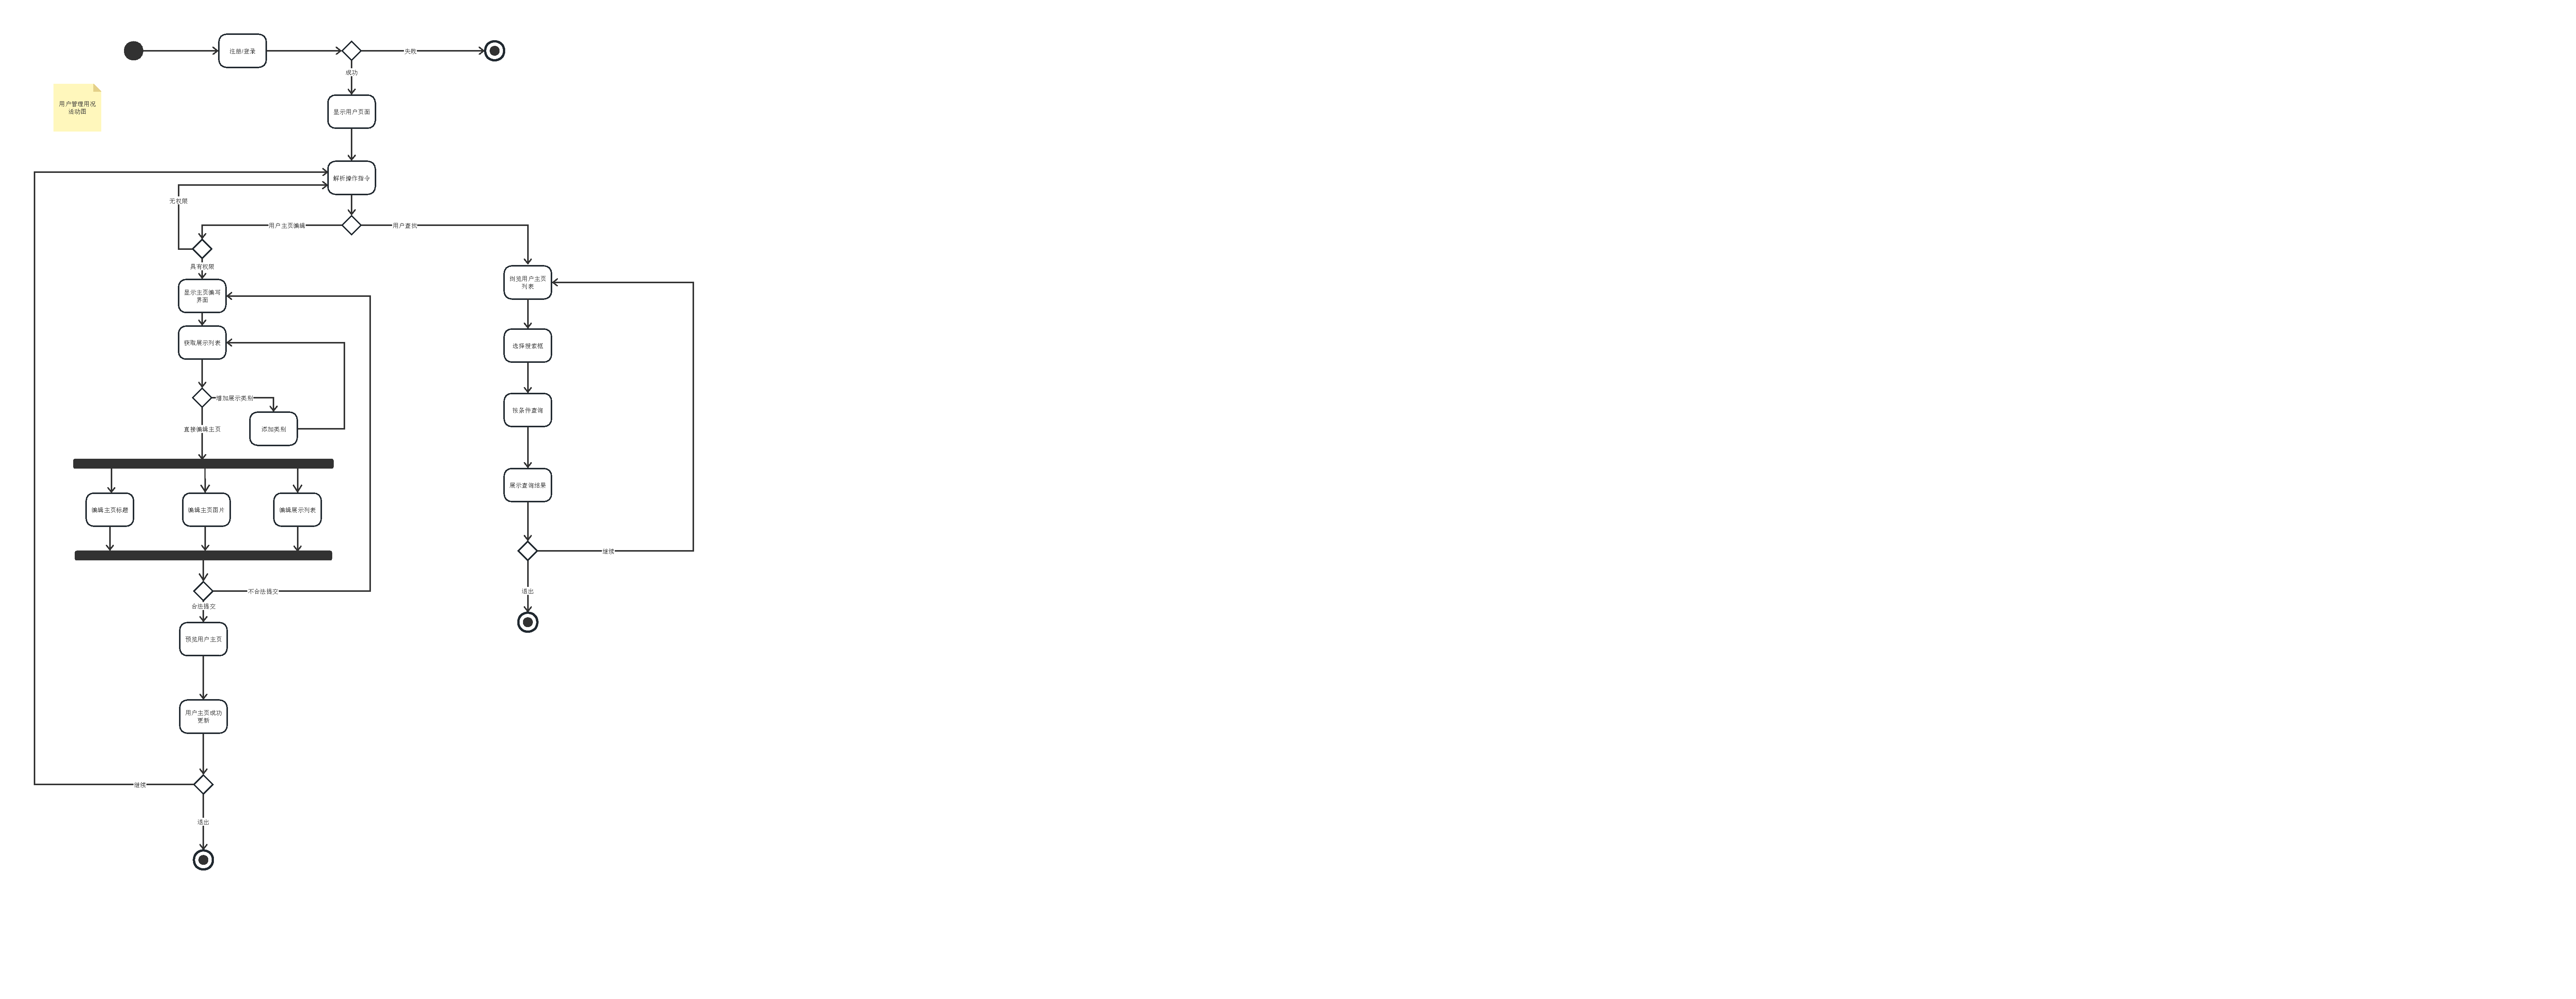
\includegraphics[scale=0.4]{OOA/fig/1-信息管理/信息管理用况活动图-1.pdf}} 
    \bicaption{Volunet信息管理系统用况活动1子图}{Activity 1 Subgraph for Information Management System Usage of Volunet} 
\end{figure}

\begin{figure}[H] 
    \center{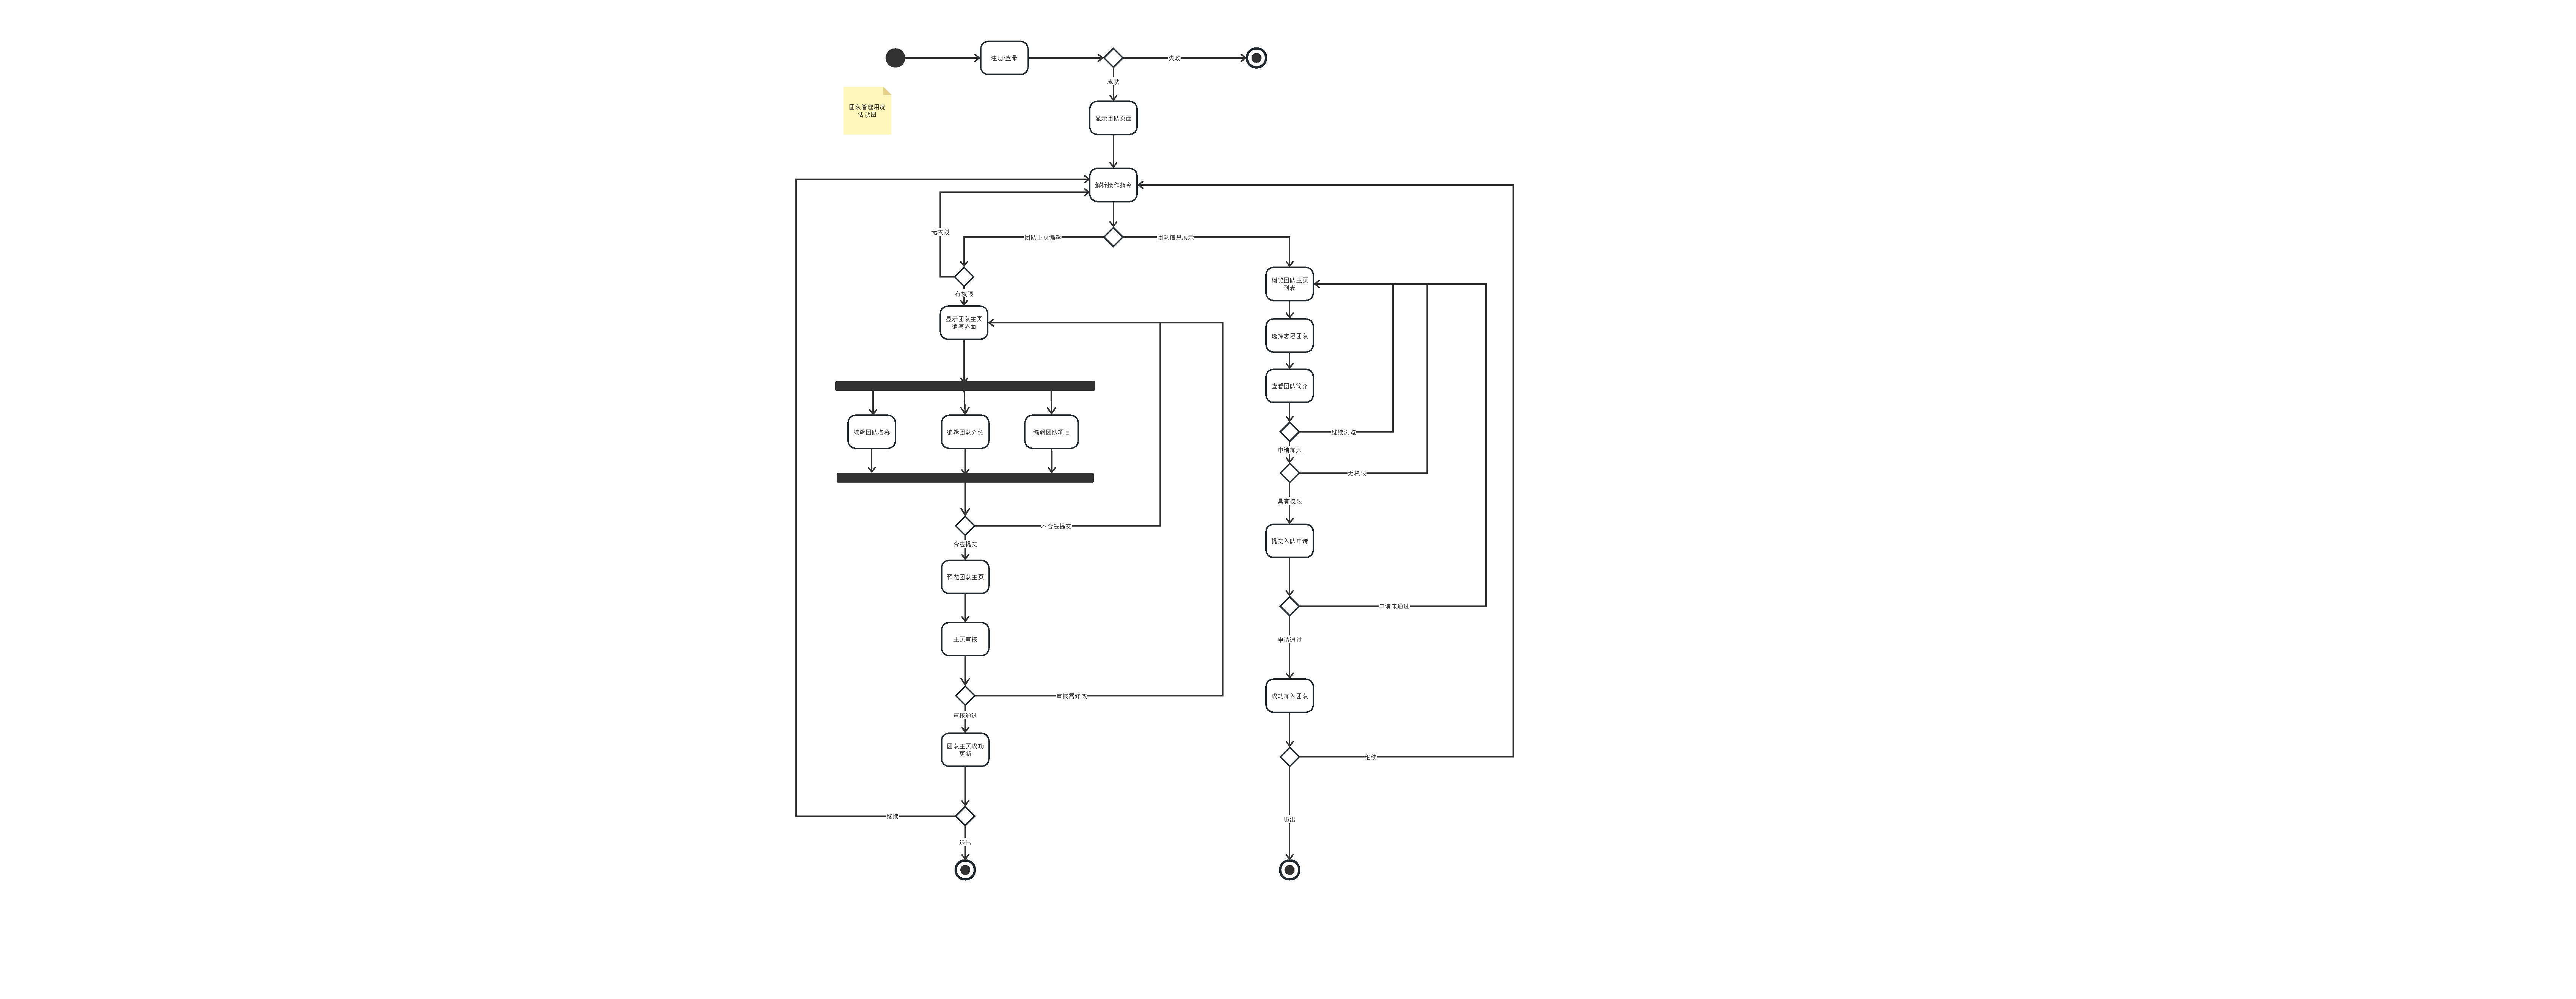
\includegraphics[scale=0.4]{OOA/fig/1-信息管理/信息管理用况活动图-2.pdf}} 
    \bicaption{Volunet信息管理系统用况活动2子图}{Activity 2 Subgraph for Information Management System Usage of Volunet} 
\end{figure}

\begin{figure}[H] 
    \center{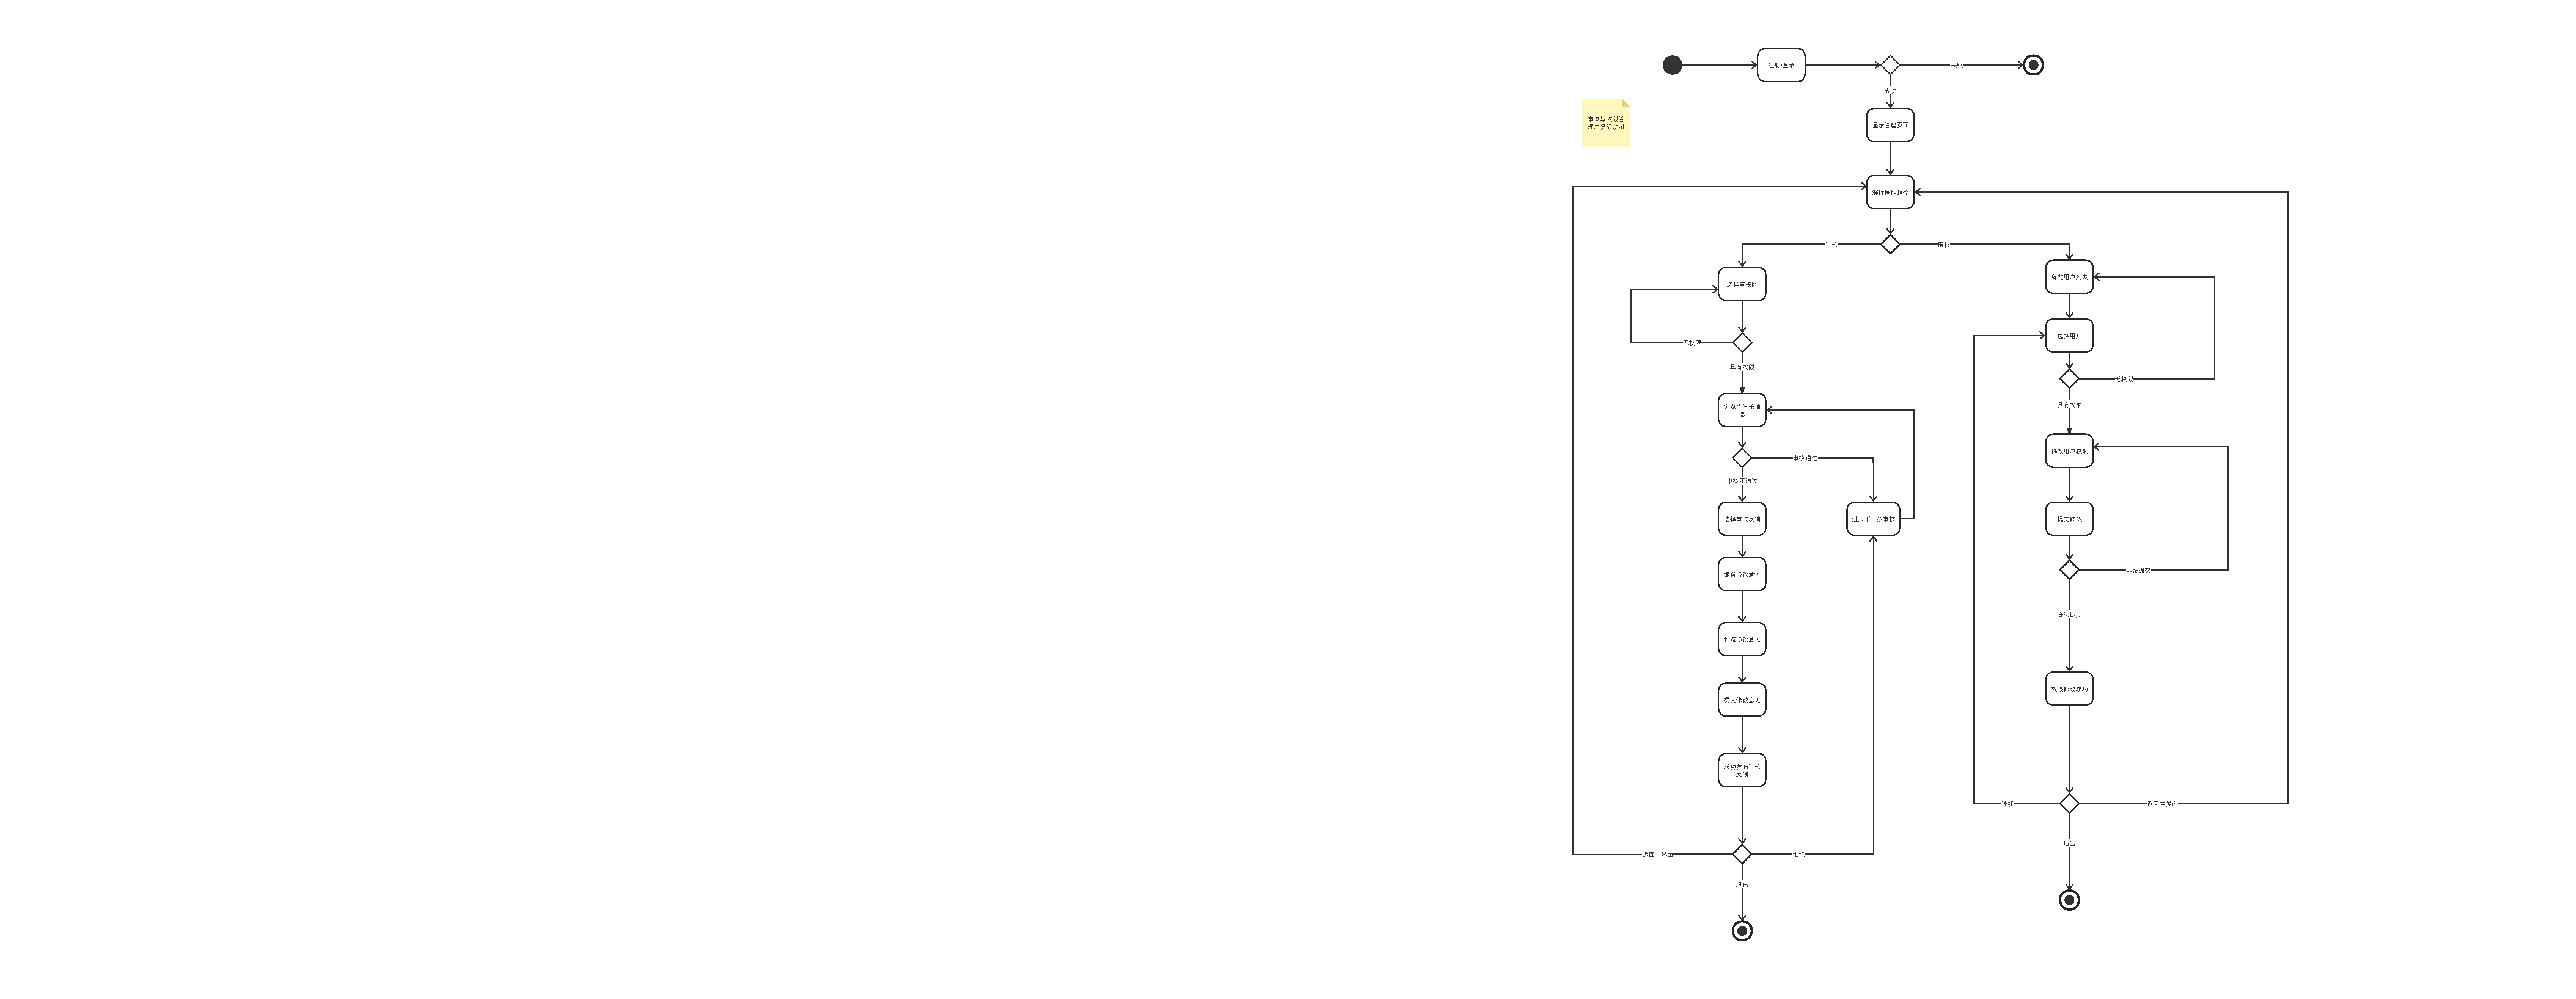
\includegraphics[scale=0.4]{OOA/fig/1-信息管理/信息管理用况活动图-3.pdf}} 
    \bicaption{Volunet信息管理系统用况活动3子图}{Activity 3 Subgraph for Information Management System Usage of Volunet} 
\end{figure}

\quad
\subsubsection{志愿服务系统}

\begin{figure}[H] 
    \center{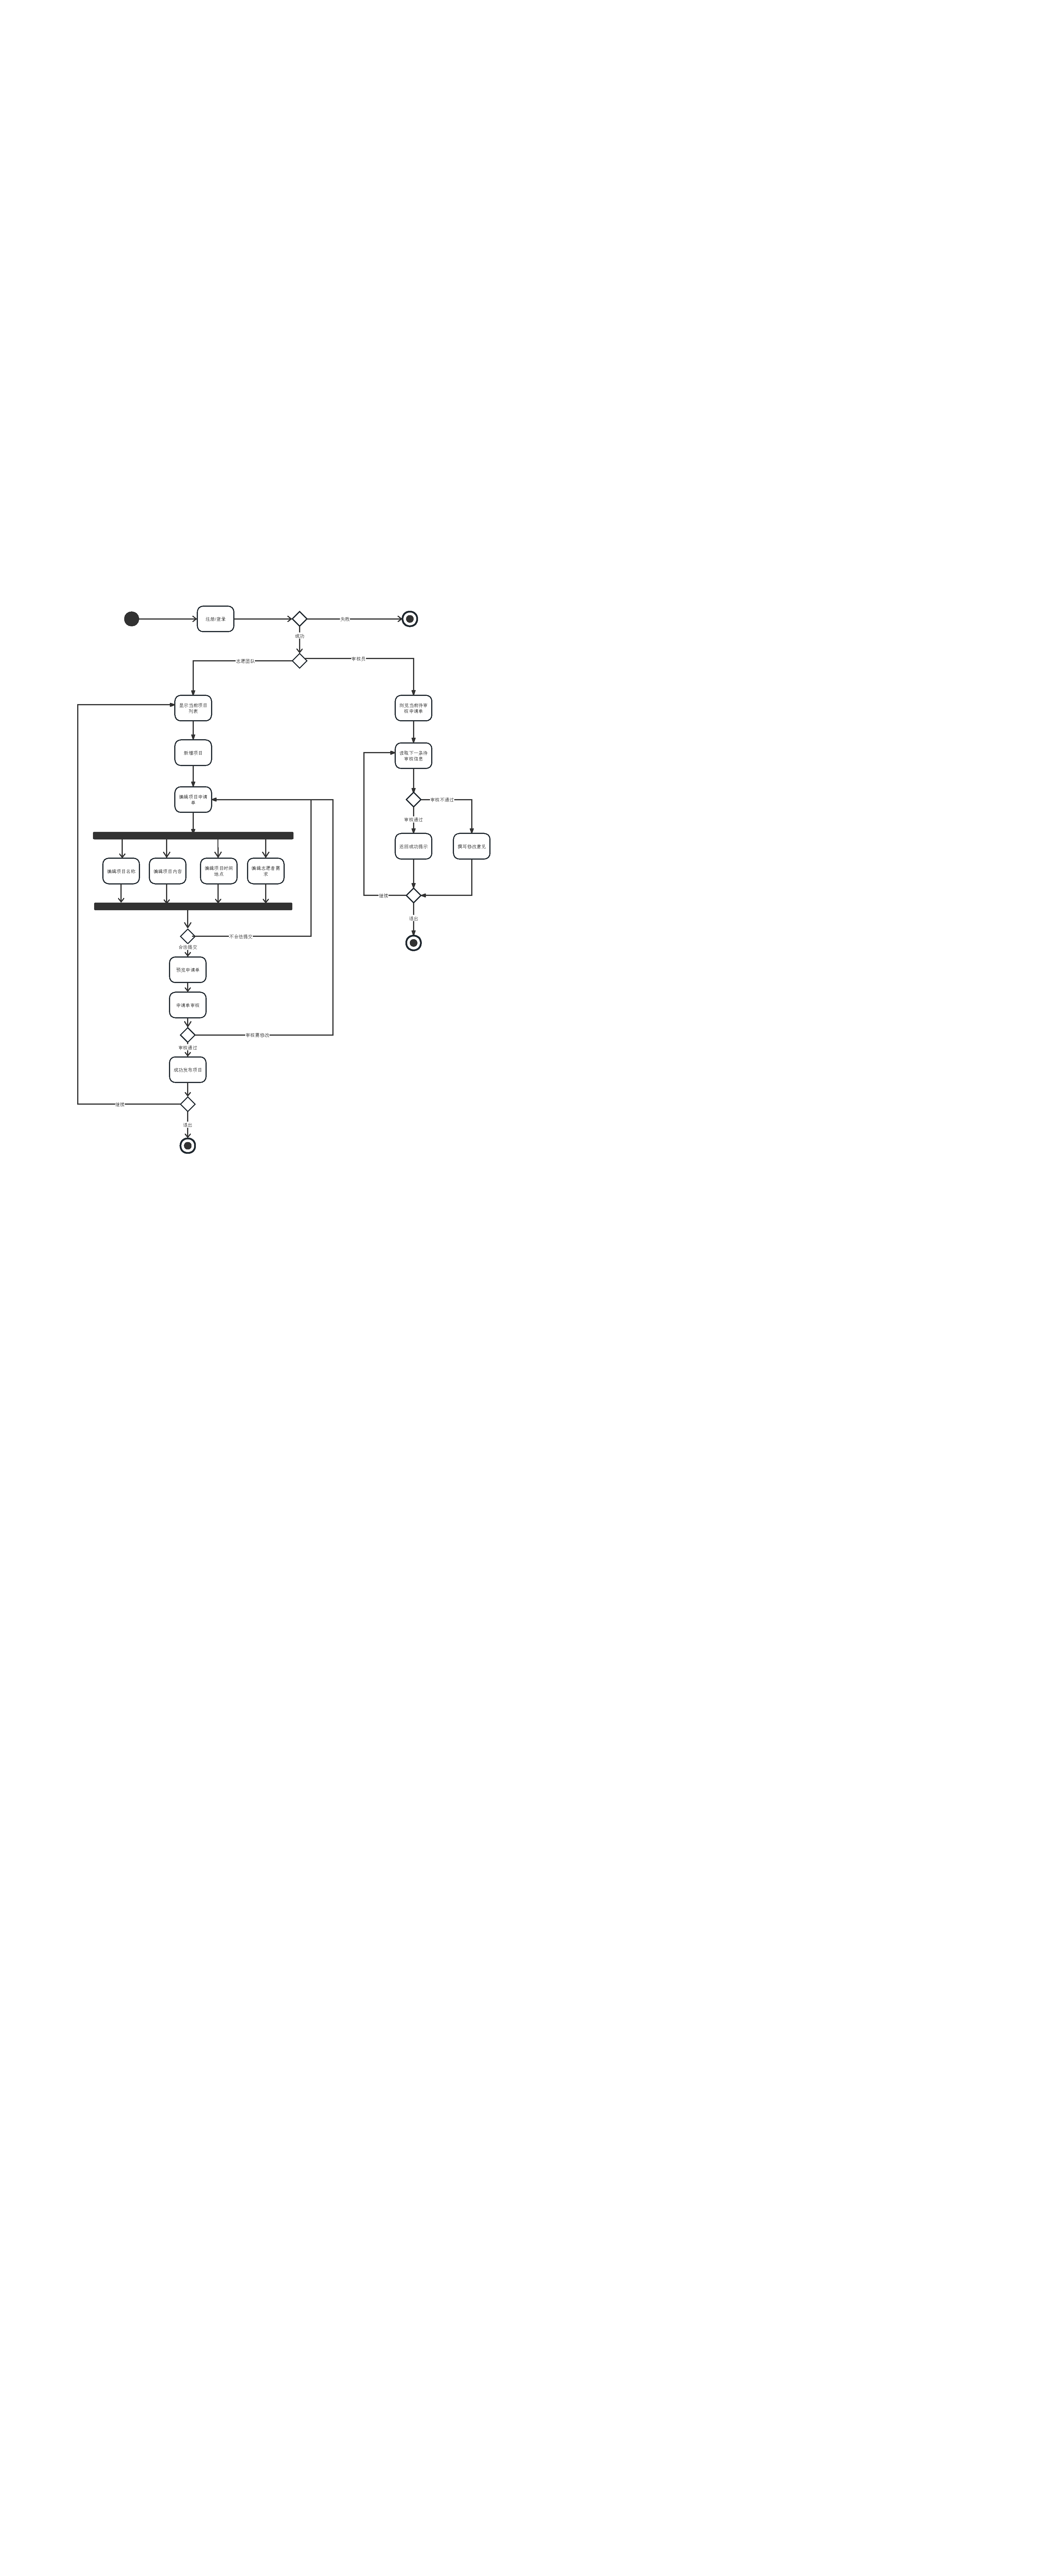
\includegraphics[scale=0.4]{OOA/fig/2-志愿服务/VS-用况活动图1.pdf}} 
    \bicaption{Volunet志愿服务系统用况活动1子图}{Activity 1 Subgraph for Voluntary Service System Usage of Volunet} 
\end{figure}

\begin{figure}[H] 
    \center{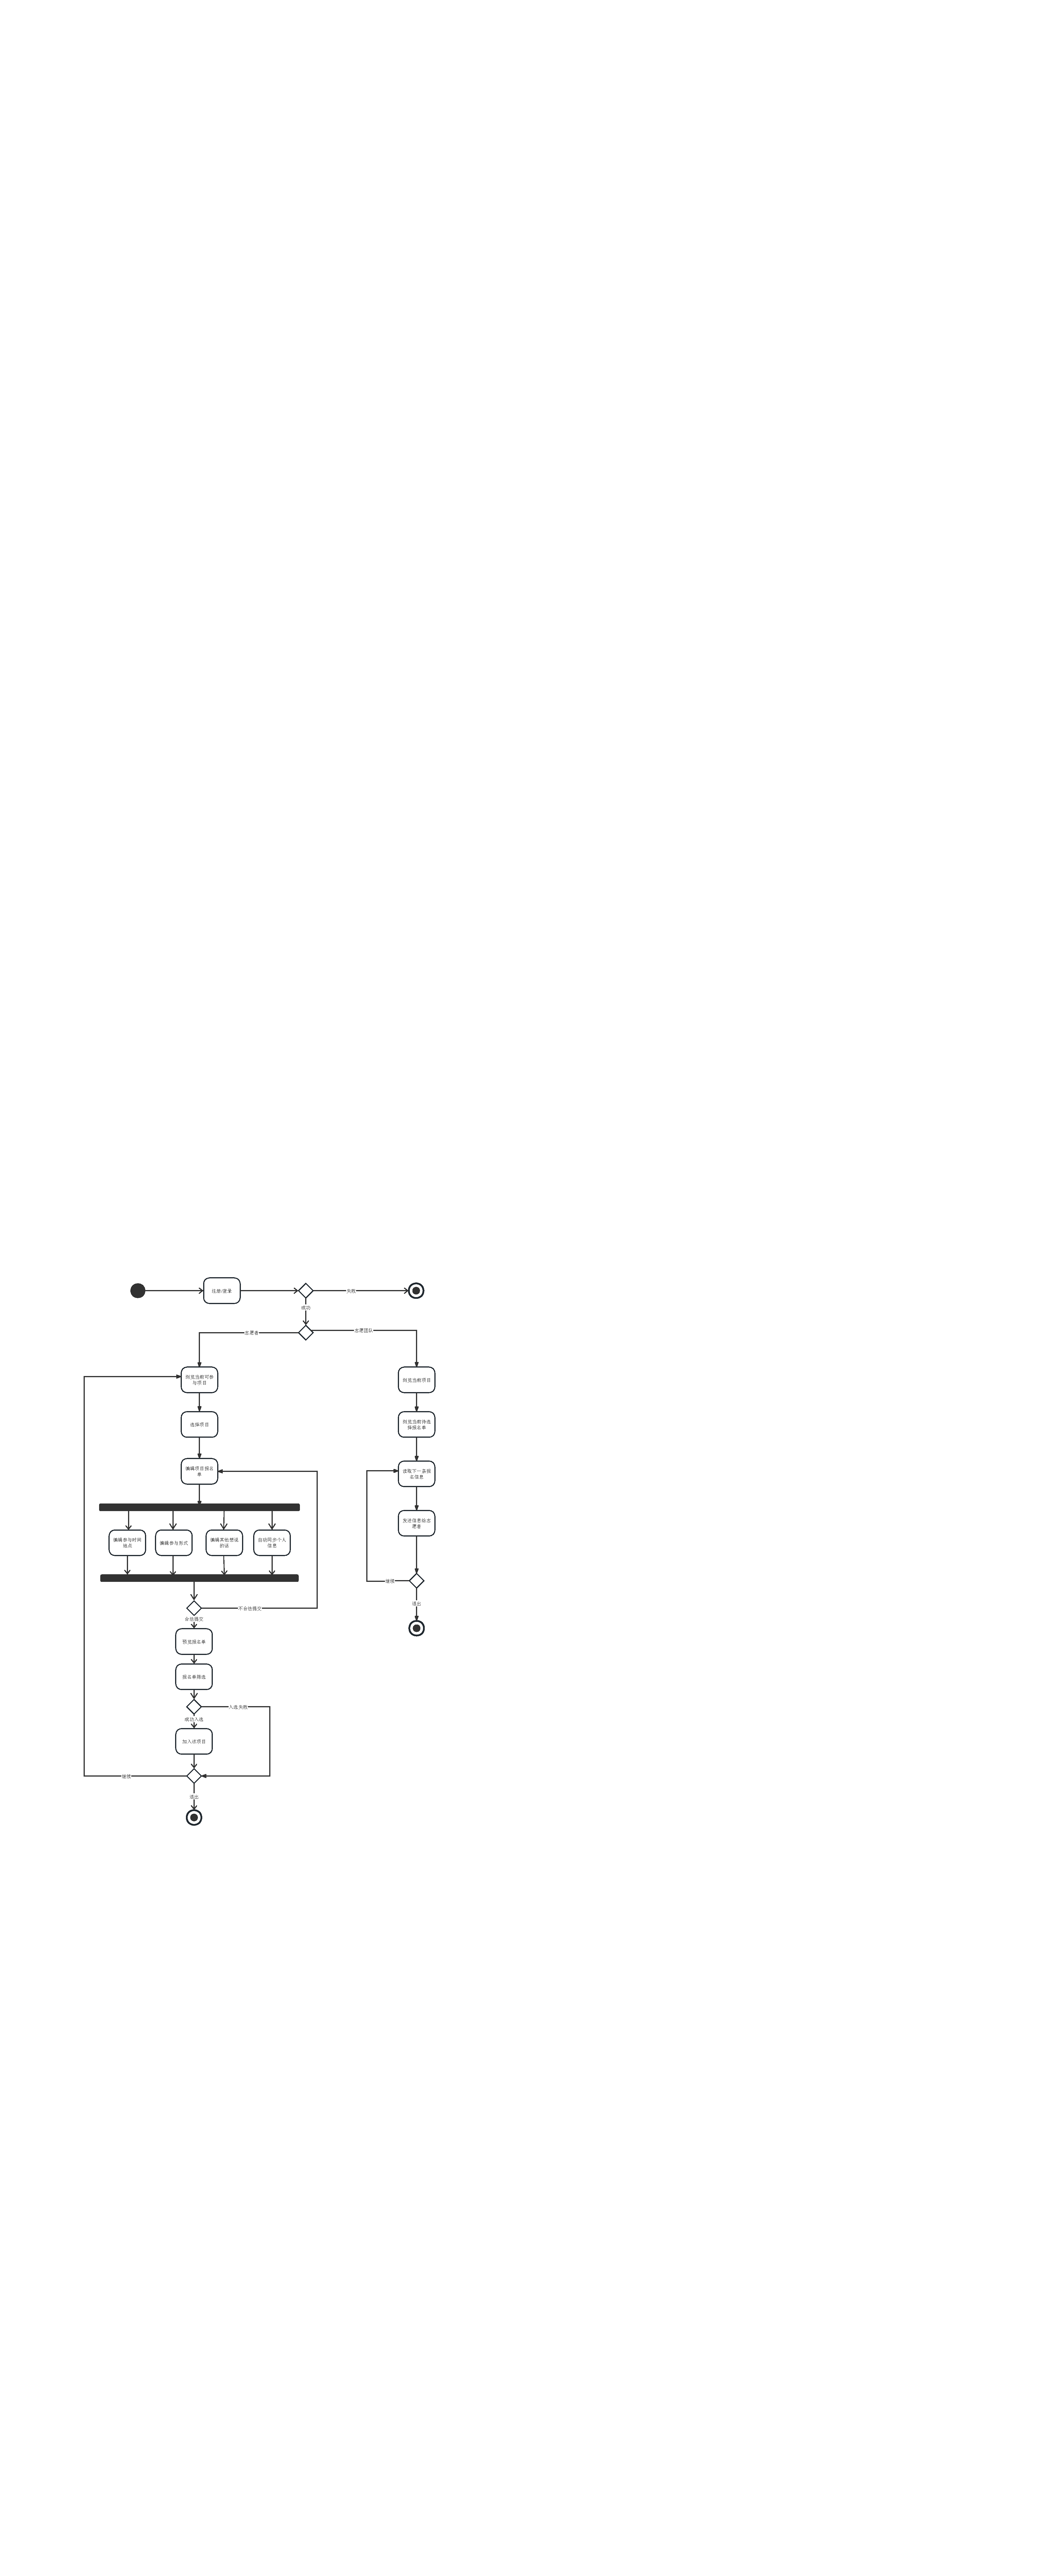
\includegraphics[scale=0.4]{OOA/fig/2-志愿服务/VS-用况活动图2.pdf}} 
    \bicaption{Volunet志愿服务系统用况活动2子图}{Activity 2 Subgraph for Voluntary Service System Usage of Volunet} 
\end{figure}

\begin{figure}[H] 
    \center{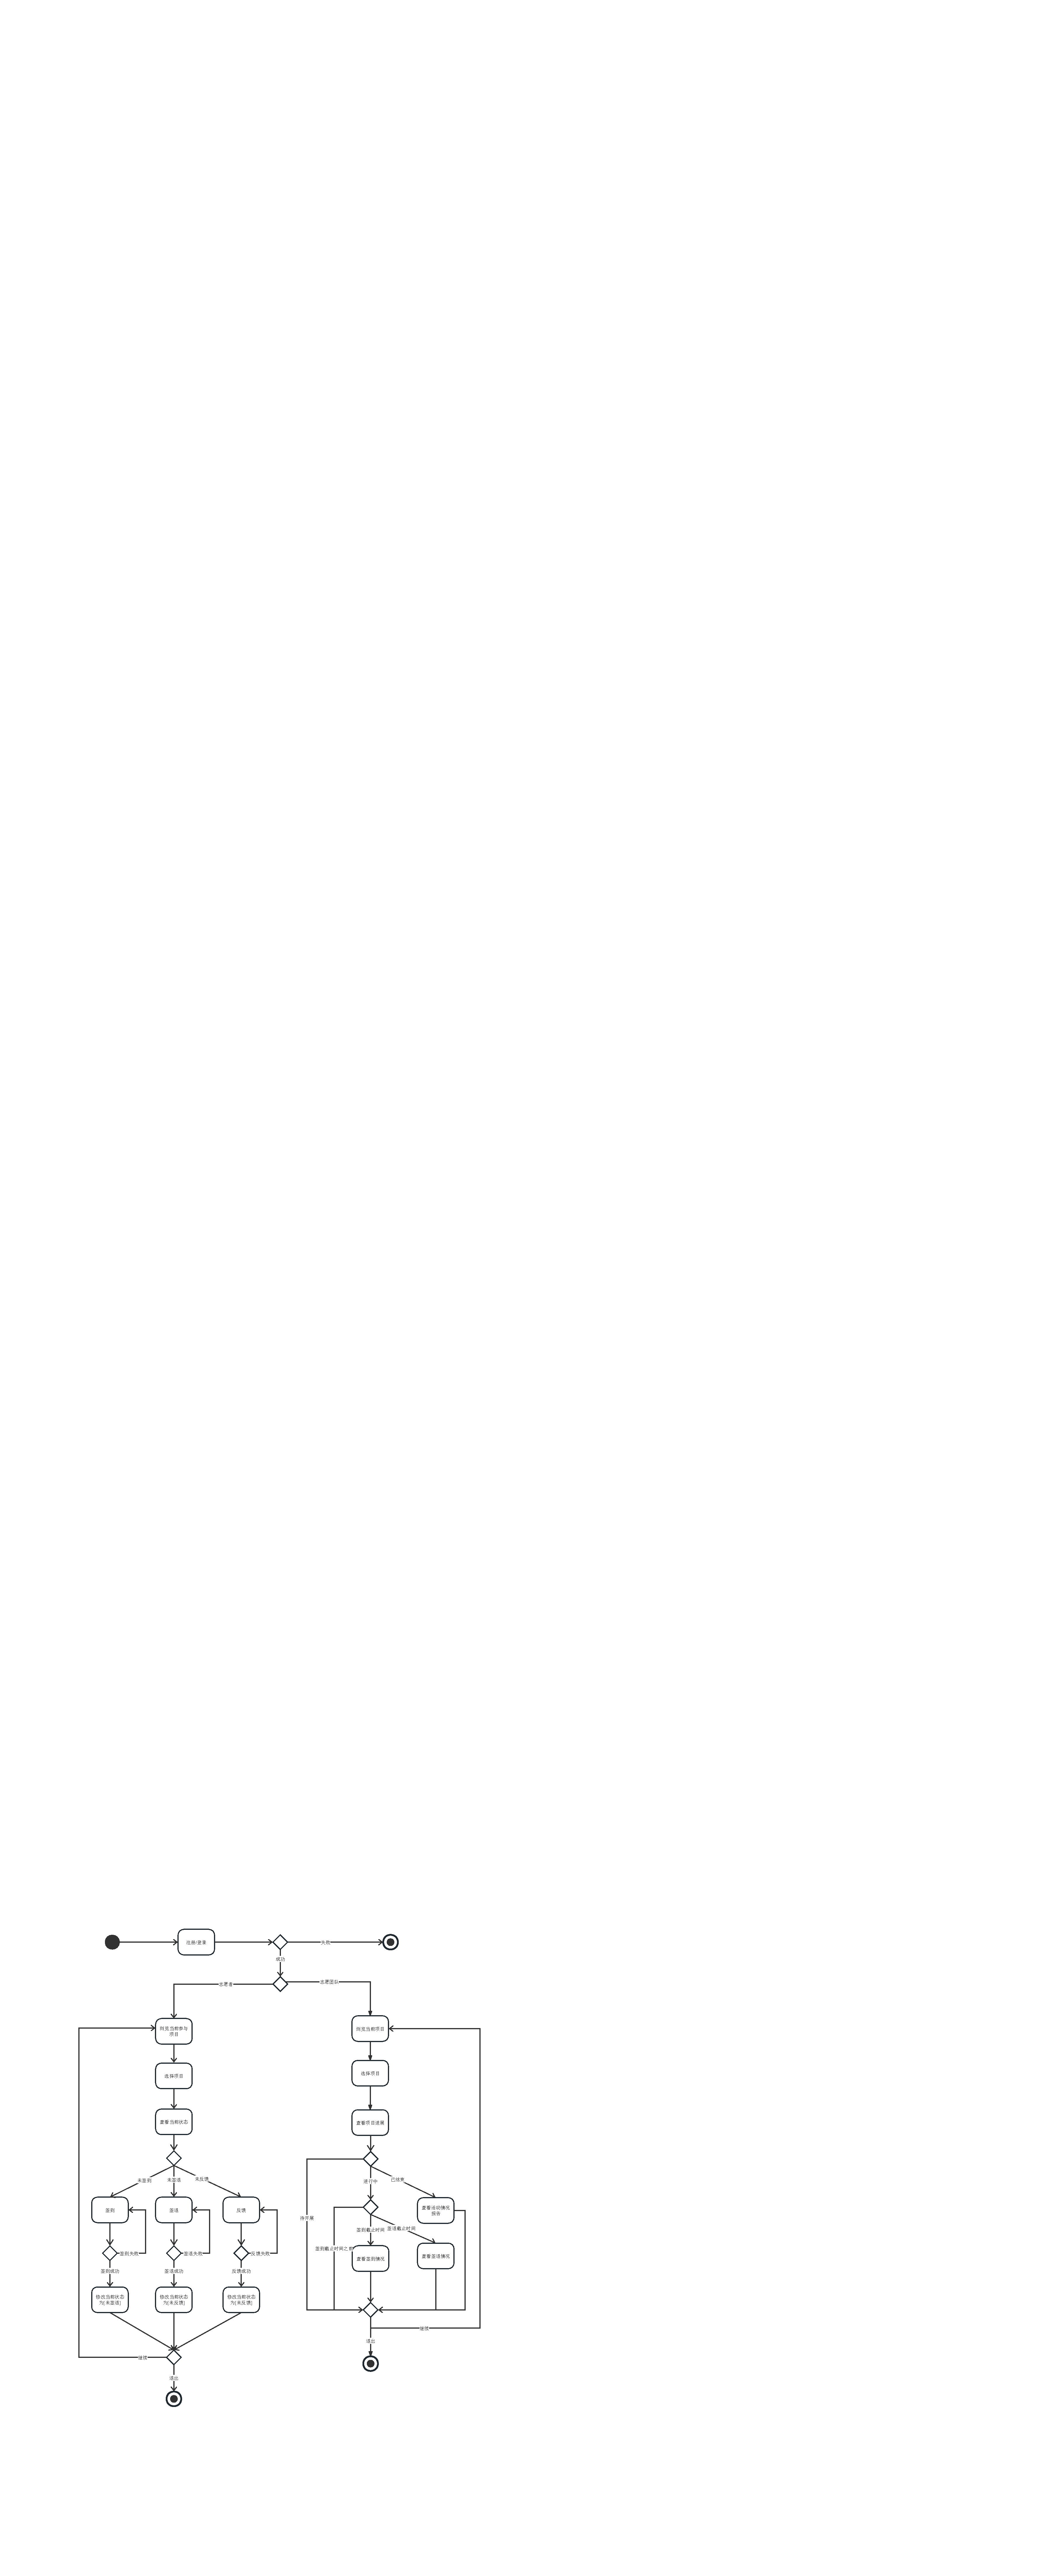
\includegraphics[scale=0.4]{OOA/fig/2-志愿服务/VS-用况活动图3.pdf}} 
    \bicaption{Volunet志愿服务系统用况活动3子图}{Activity 3 Subgraph for Voluntary Service System Usage of Volunet} 
\end{figure}


\subsubsection{爱心捐助系统}
\begin{figure}[H] 
    \center{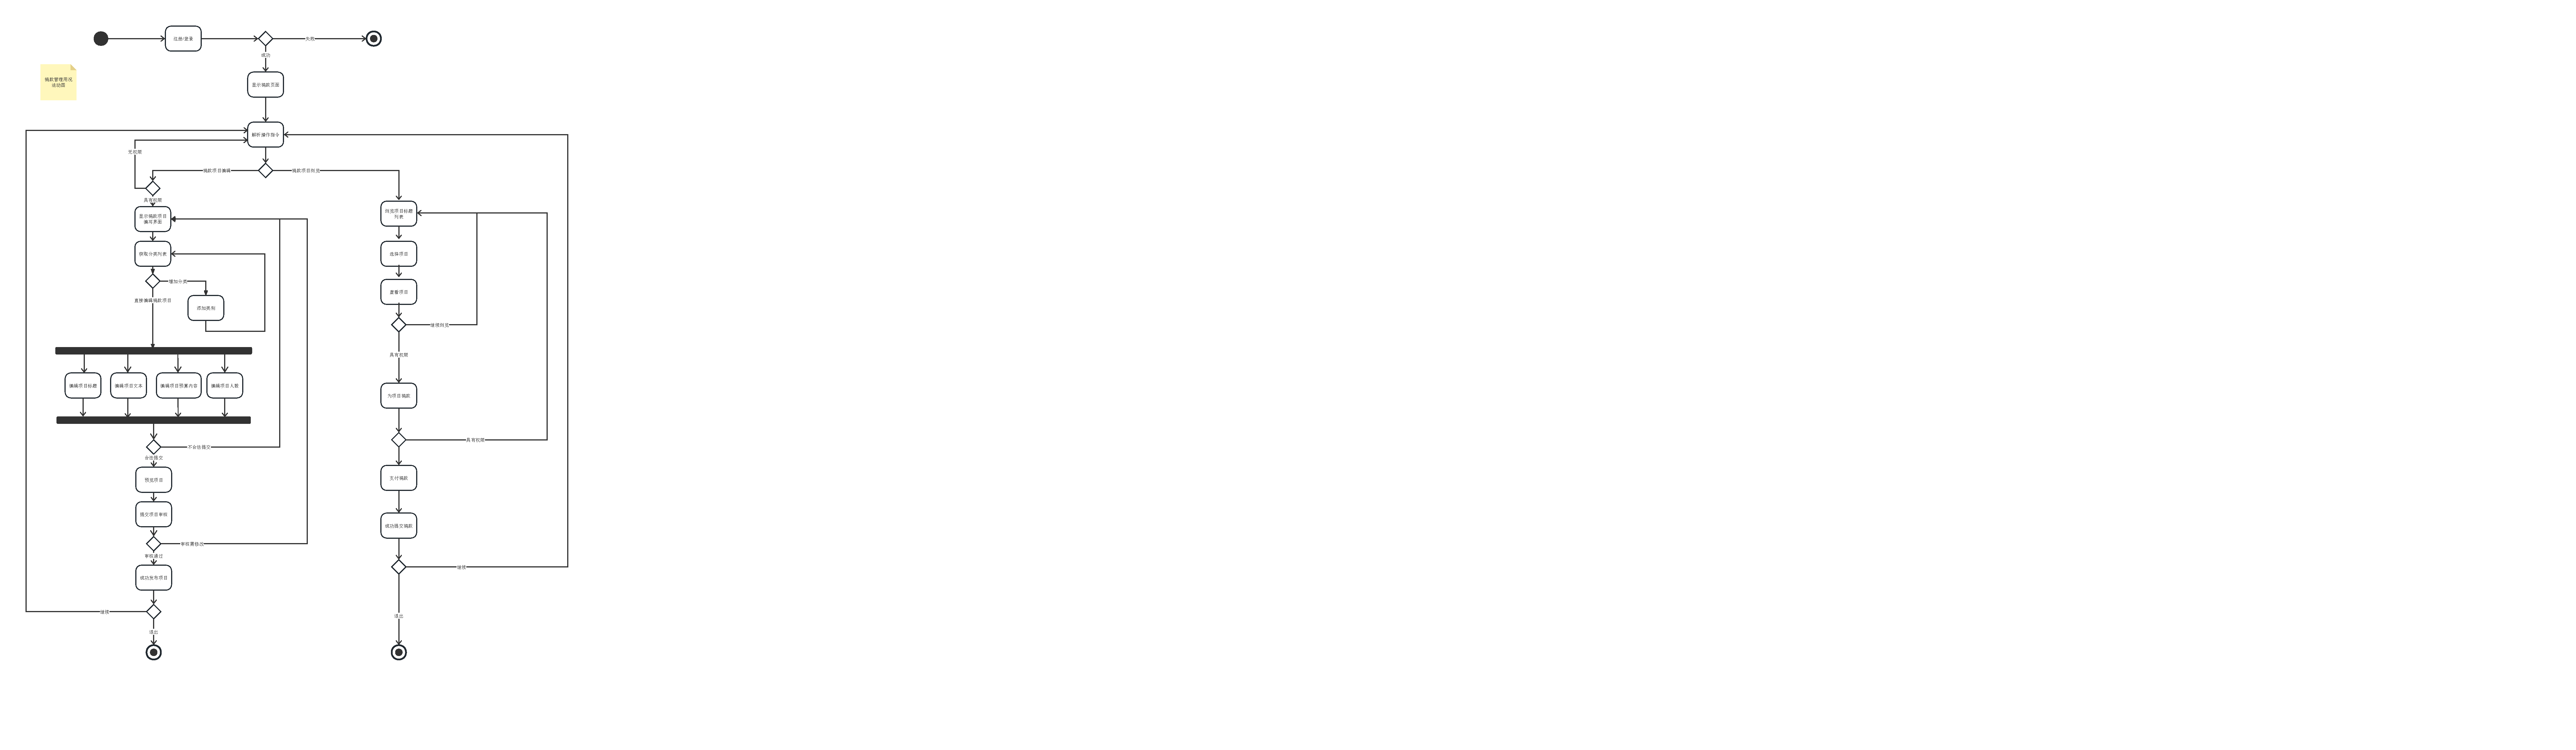
\includegraphics[scale=0.4]{OOA/fig/3-爱心管理/爱心管理用况活动图-1.pdf}} 
    \bicaption{Volunet爱心捐助系统用况活动1子图}{Activity 1 Subgraph for Love Donation System Usage of Volunet} 
\end{figure}
\quad
\begin{figure}[H] 
    \center{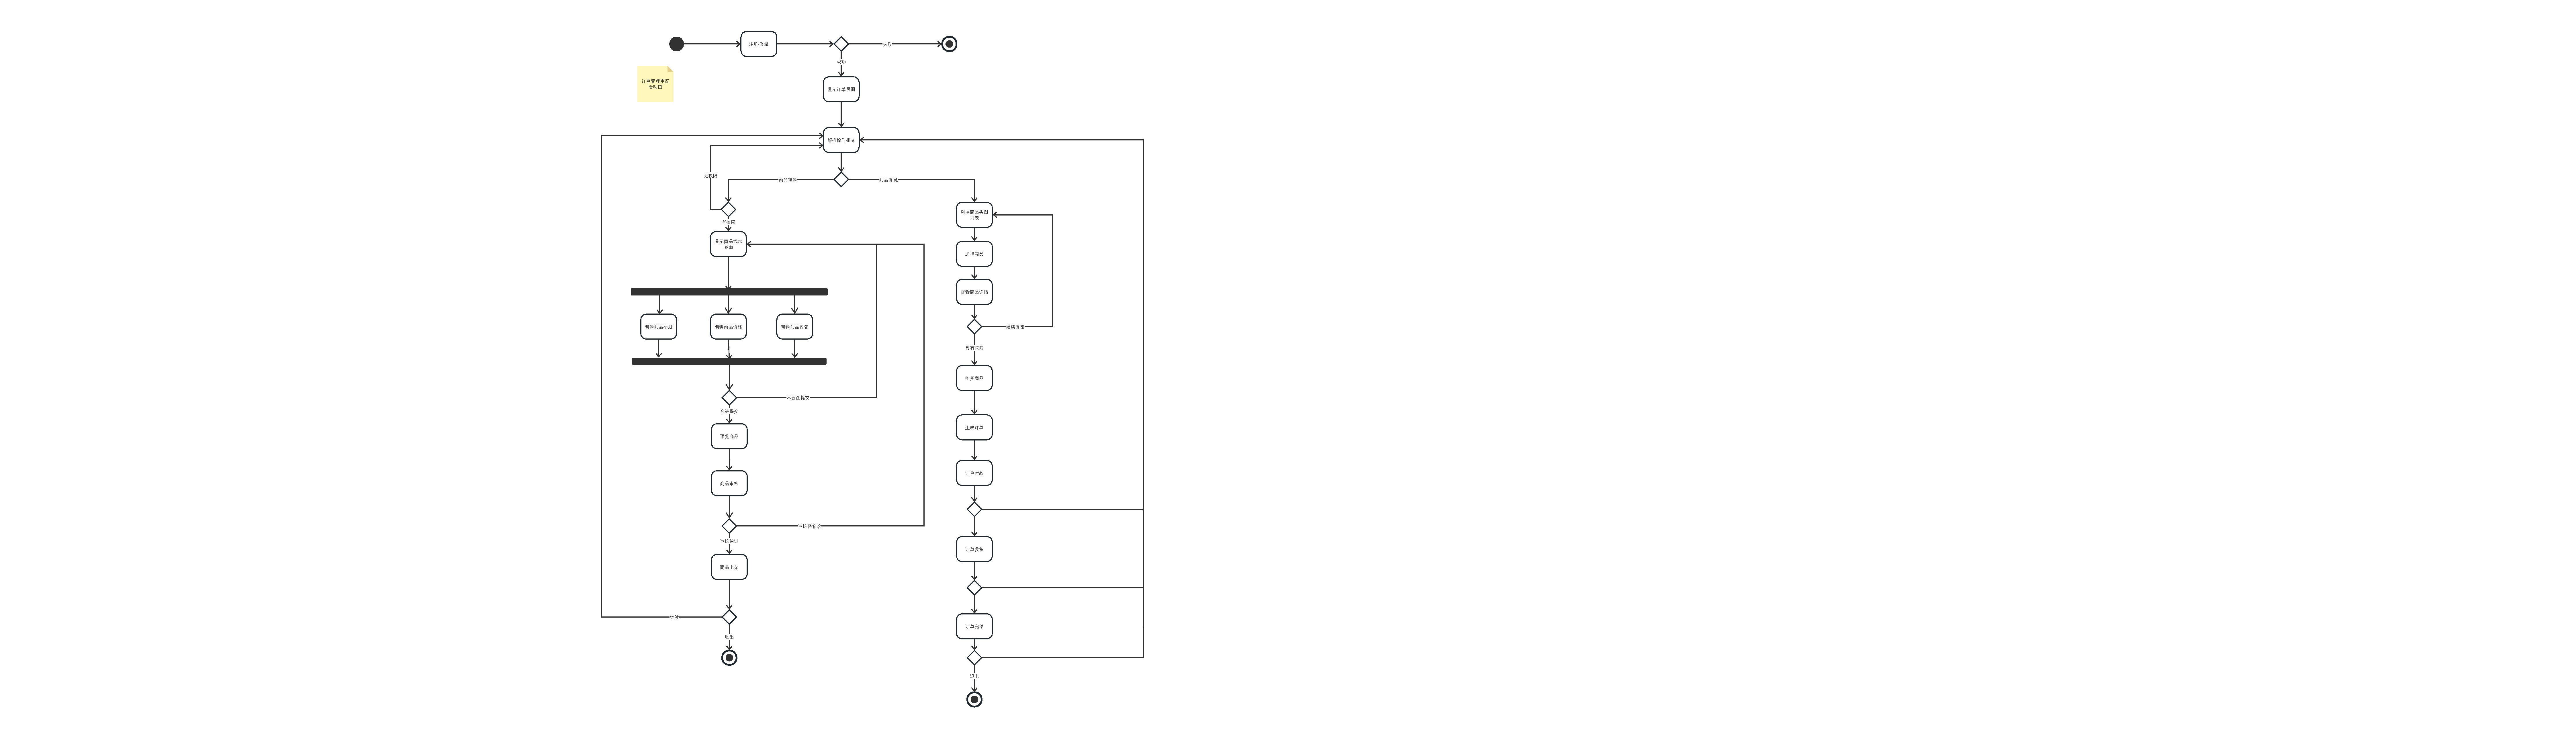
\includegraphics[scale=0.4]{OOA/fig/3-爱心管理/爱心管理用况活动图-2.pdf}} 
    \bicaption{Volunet爱心捐助系统用况活动2子图}{Activity 2 Subgraph for Love Donation System Usage of Volunet} 
\end{figure}

\begin{figure}[H] 
    \center{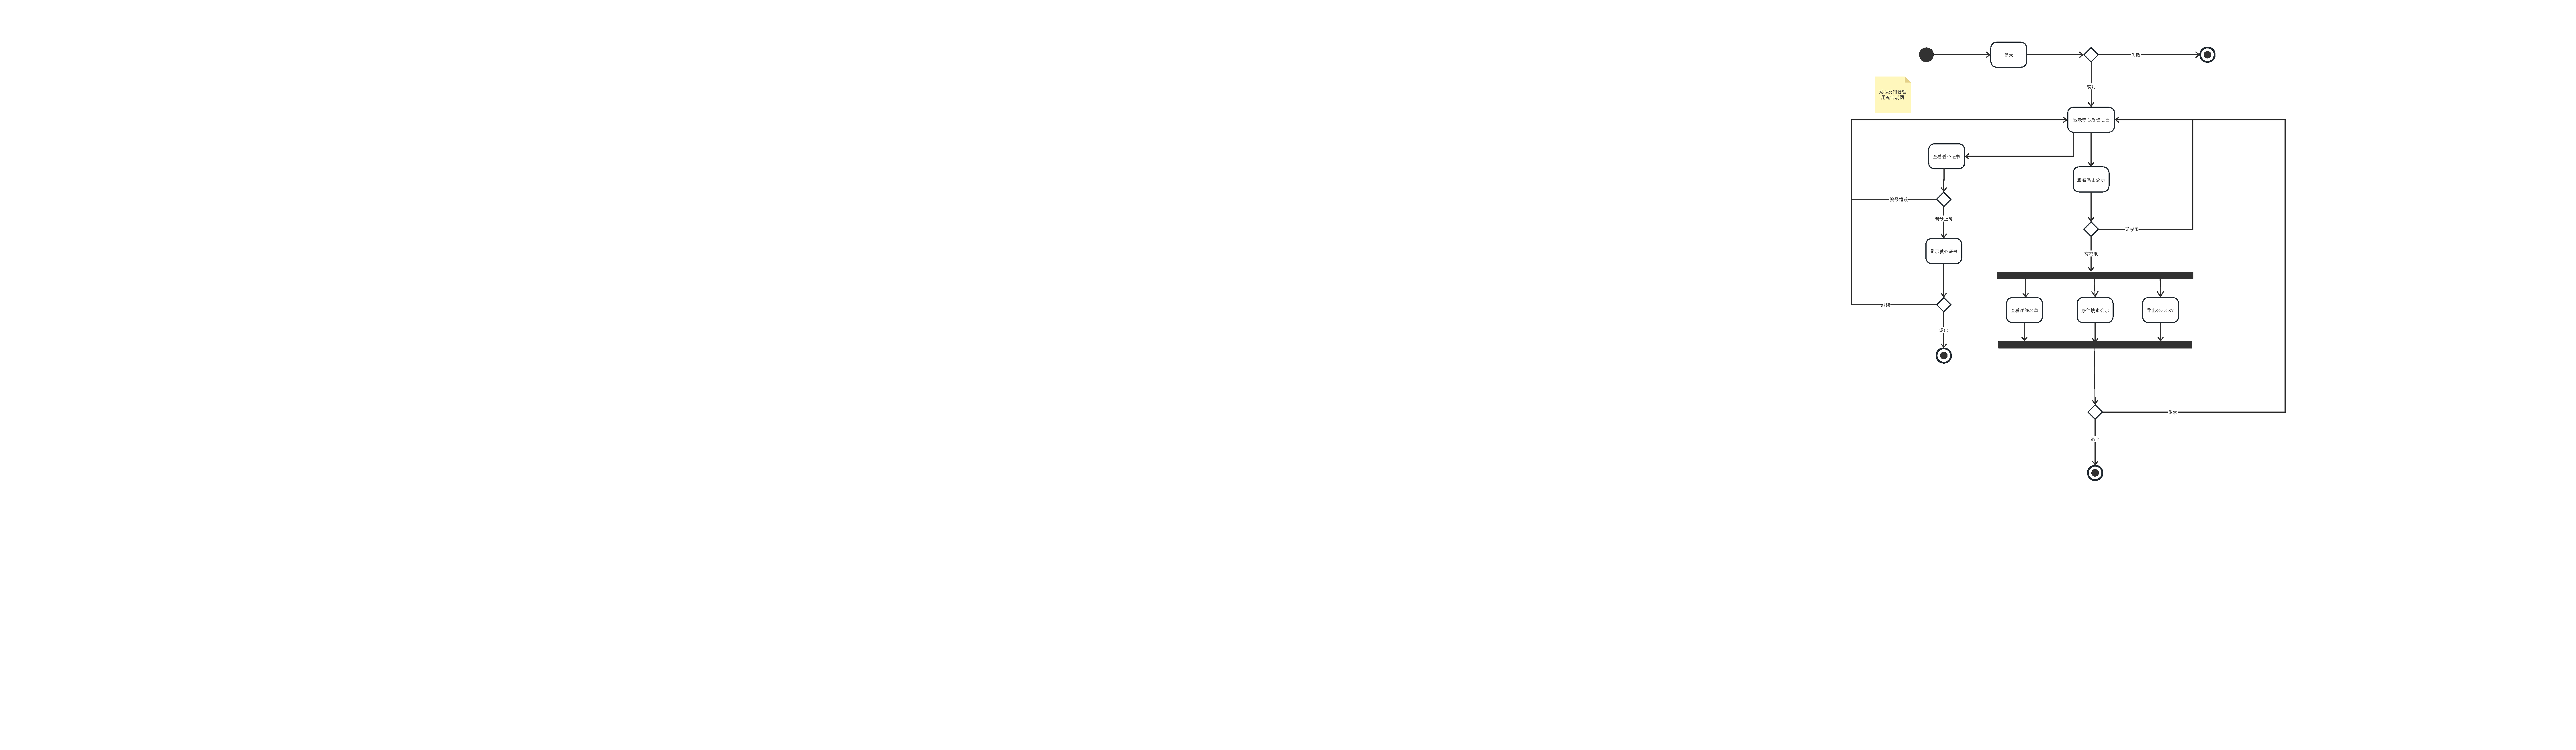
\includegraphics[scale=0.5]{OOA/fig/3-爱心管理/爱心管理用况活动图-3.pdf}} 
    \bicaption{Volunet爱心捐助系统用况活动3子图}{Activity 3 Subgraph for Love Donation System Usage of Volunet} 
\end{figure}

\subsubsection{公益课程系统}
\begin{figure}[H] 
    \center{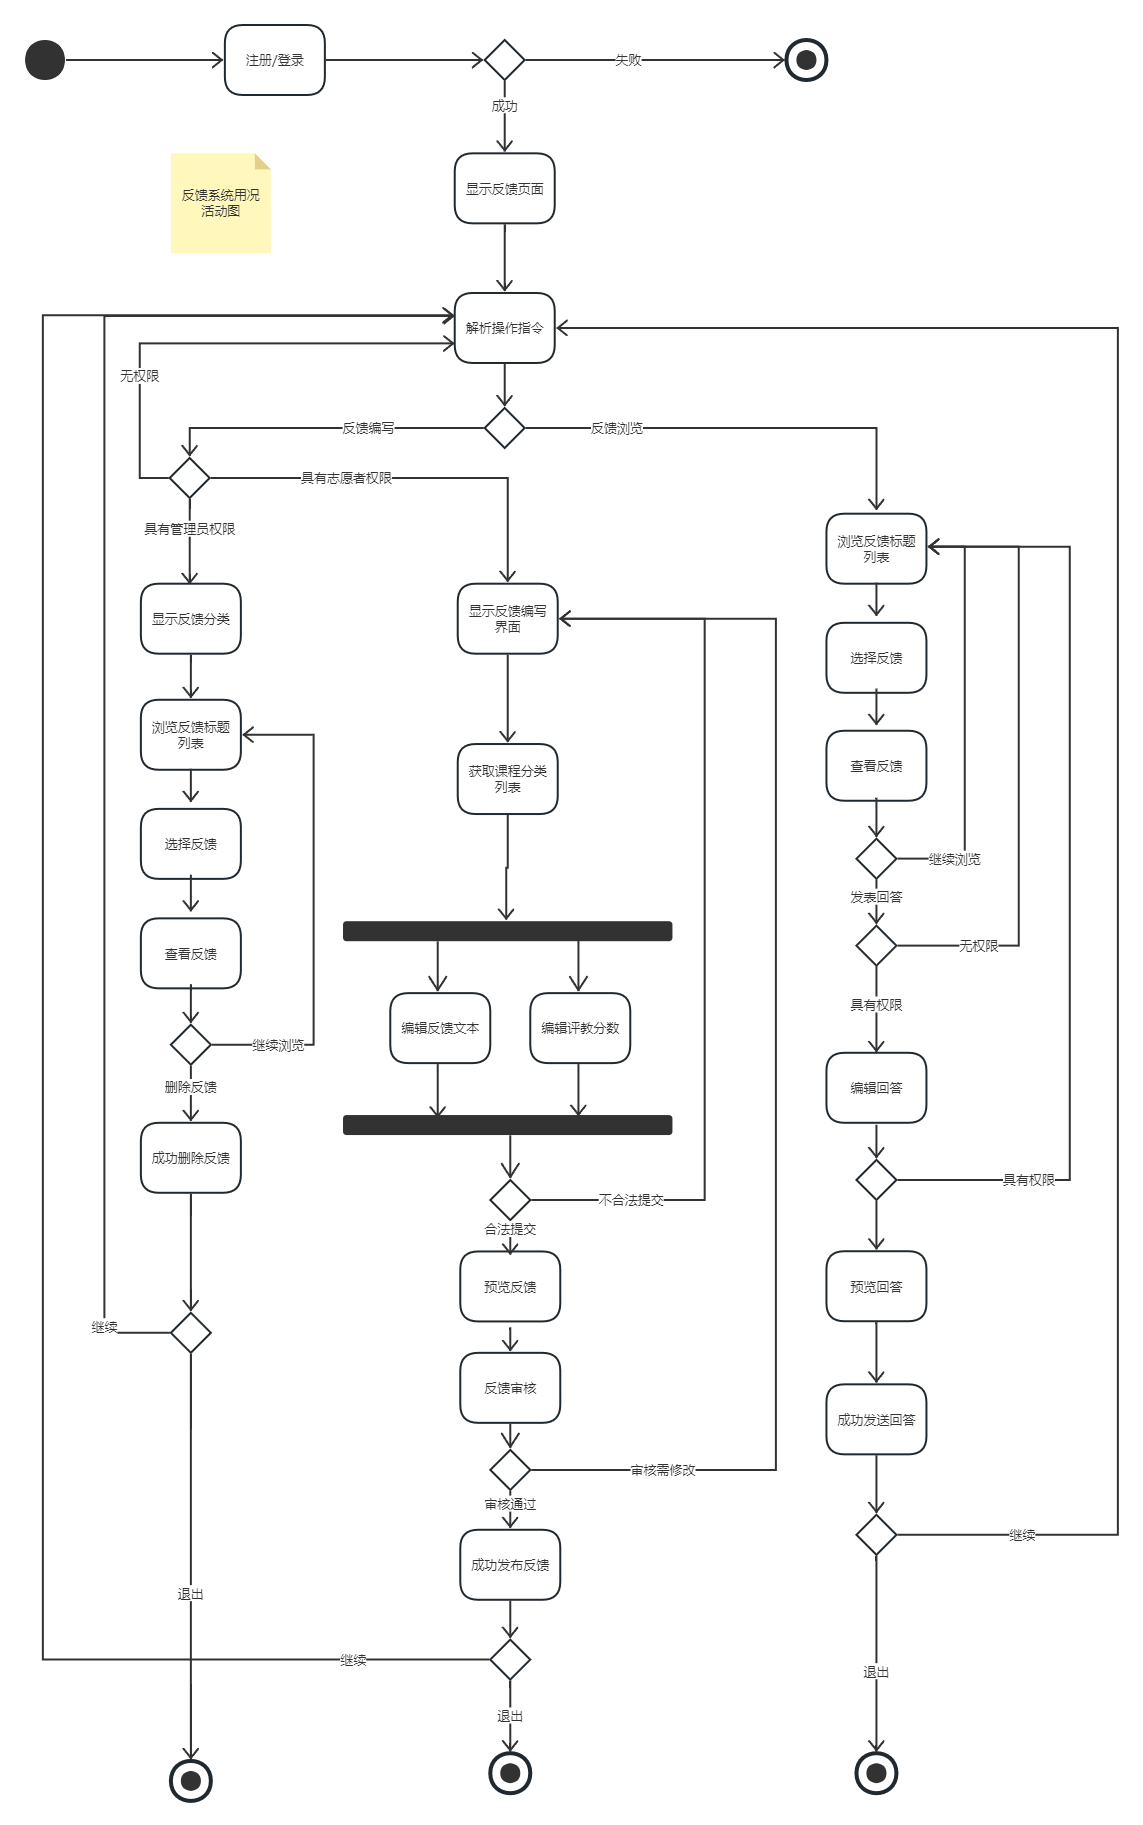
\includegraphics[scale=0.25]{OOA/fig/4-课程管理/课程管理用况活动图.png}} 
    \bicaption{Volunet公益课程系统用况活动1子图}{Activity 1 Subgraph for Course System Usage of Volunet} 
\end{figure}

\begin{figure}[H] 
    \center{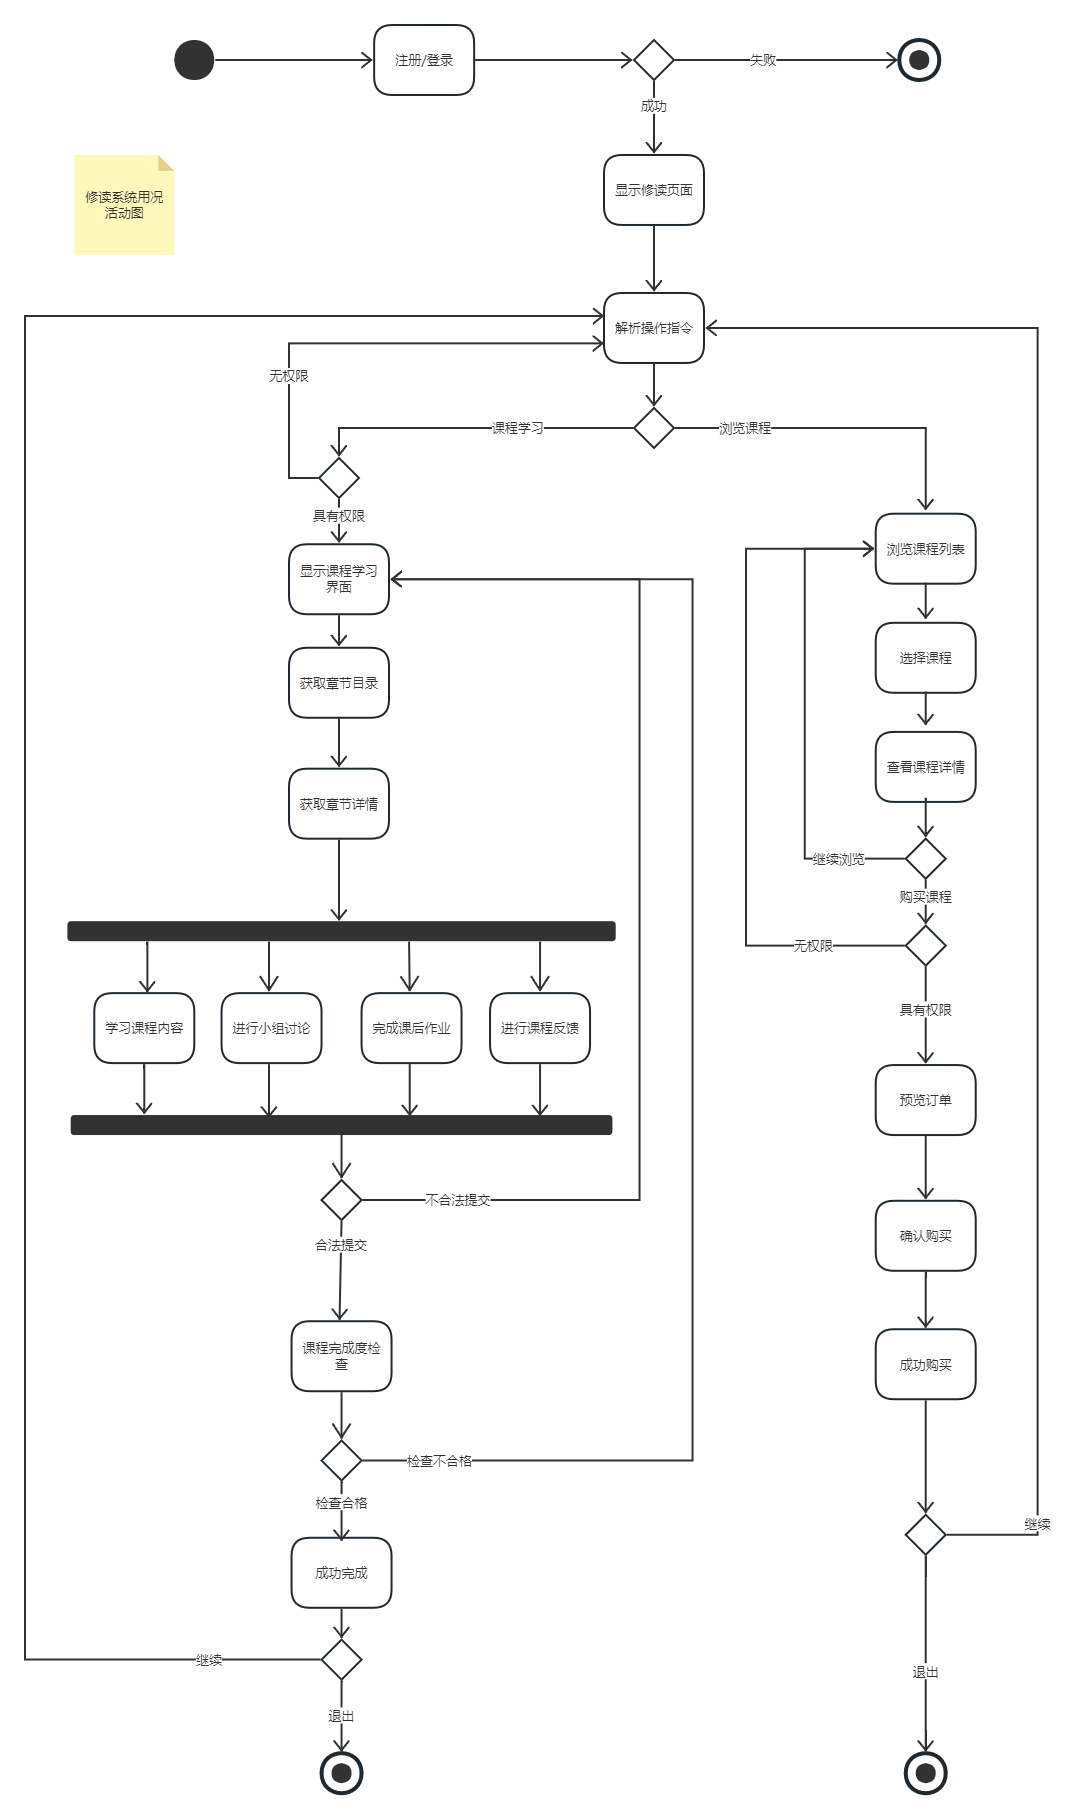
\includegraphics[scale=0.35]{OOA/fig/4-课程管理/课程管理用况活动图 (1).png}} 
    \bicaption{Volunet公益课程系统用况活动2子图}{Activity 2 Subgraph for Course System Usage of Volunet} 
\end{figure}

\begin{figure}[H] 
    \center{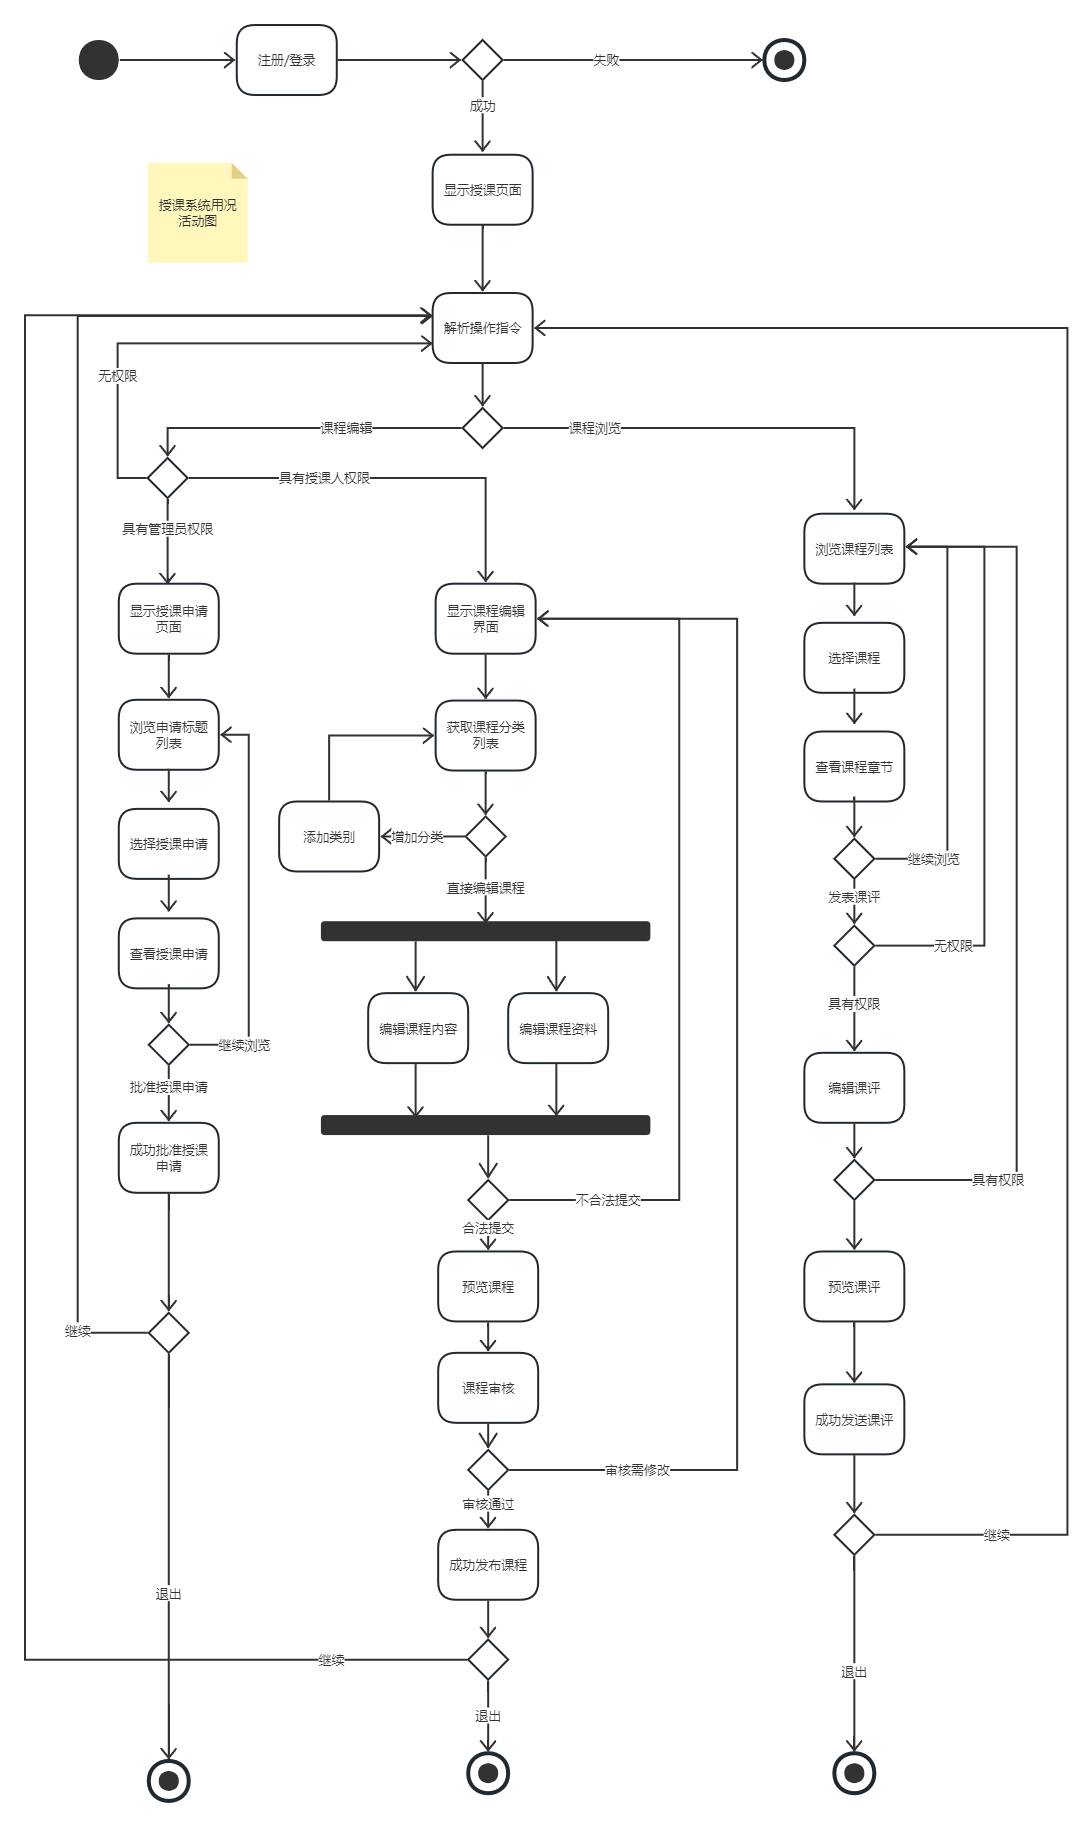
\includegraphics[scale=0.35]{OOA/fig/4-课程管理/课程管理用况活动图 (2).png}} 
    \bicaption{Volunet公益课程系统用况活动3子图}{Activity 3 Subgraph for Course System Usage of Volunet} 
\end{figure}

\subsubsection{交流论坛系统}
\begin{figure}[H] 
    \center{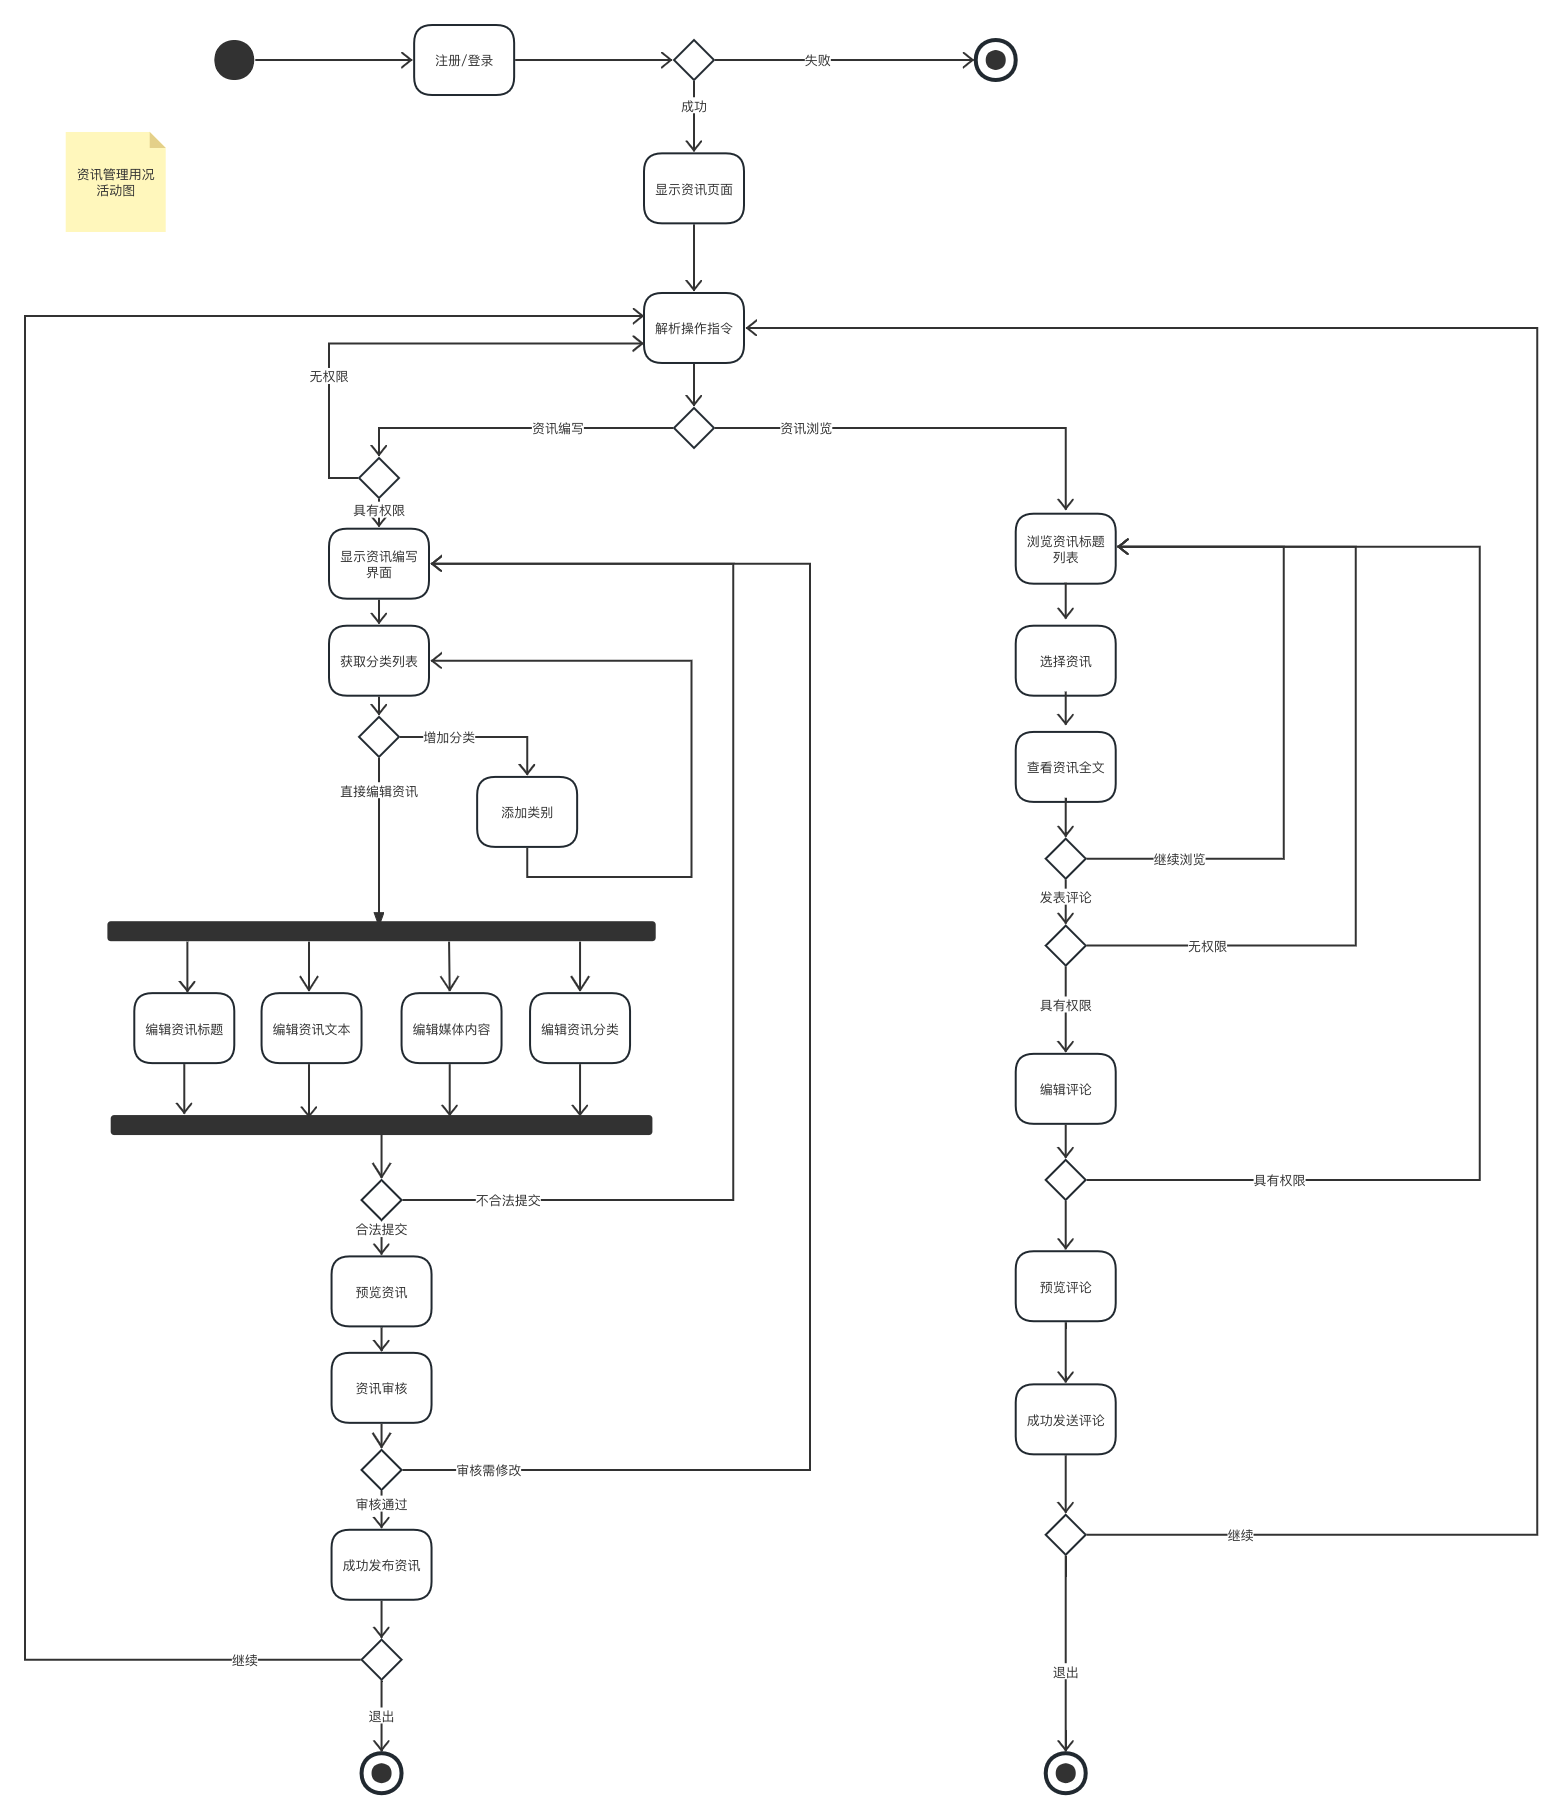
\includegraphics[scale=0.25]{OOA/fig/5-论坛管理/论坛管理用况活动图-1.png}} 
    \bicaption{Volunet交流论坛系统用况活动1子图}{Activity 1 Subgraph for Communication System Use Case of Volunet} 
\end{figure}

\begin{figure}[H] 
    \center{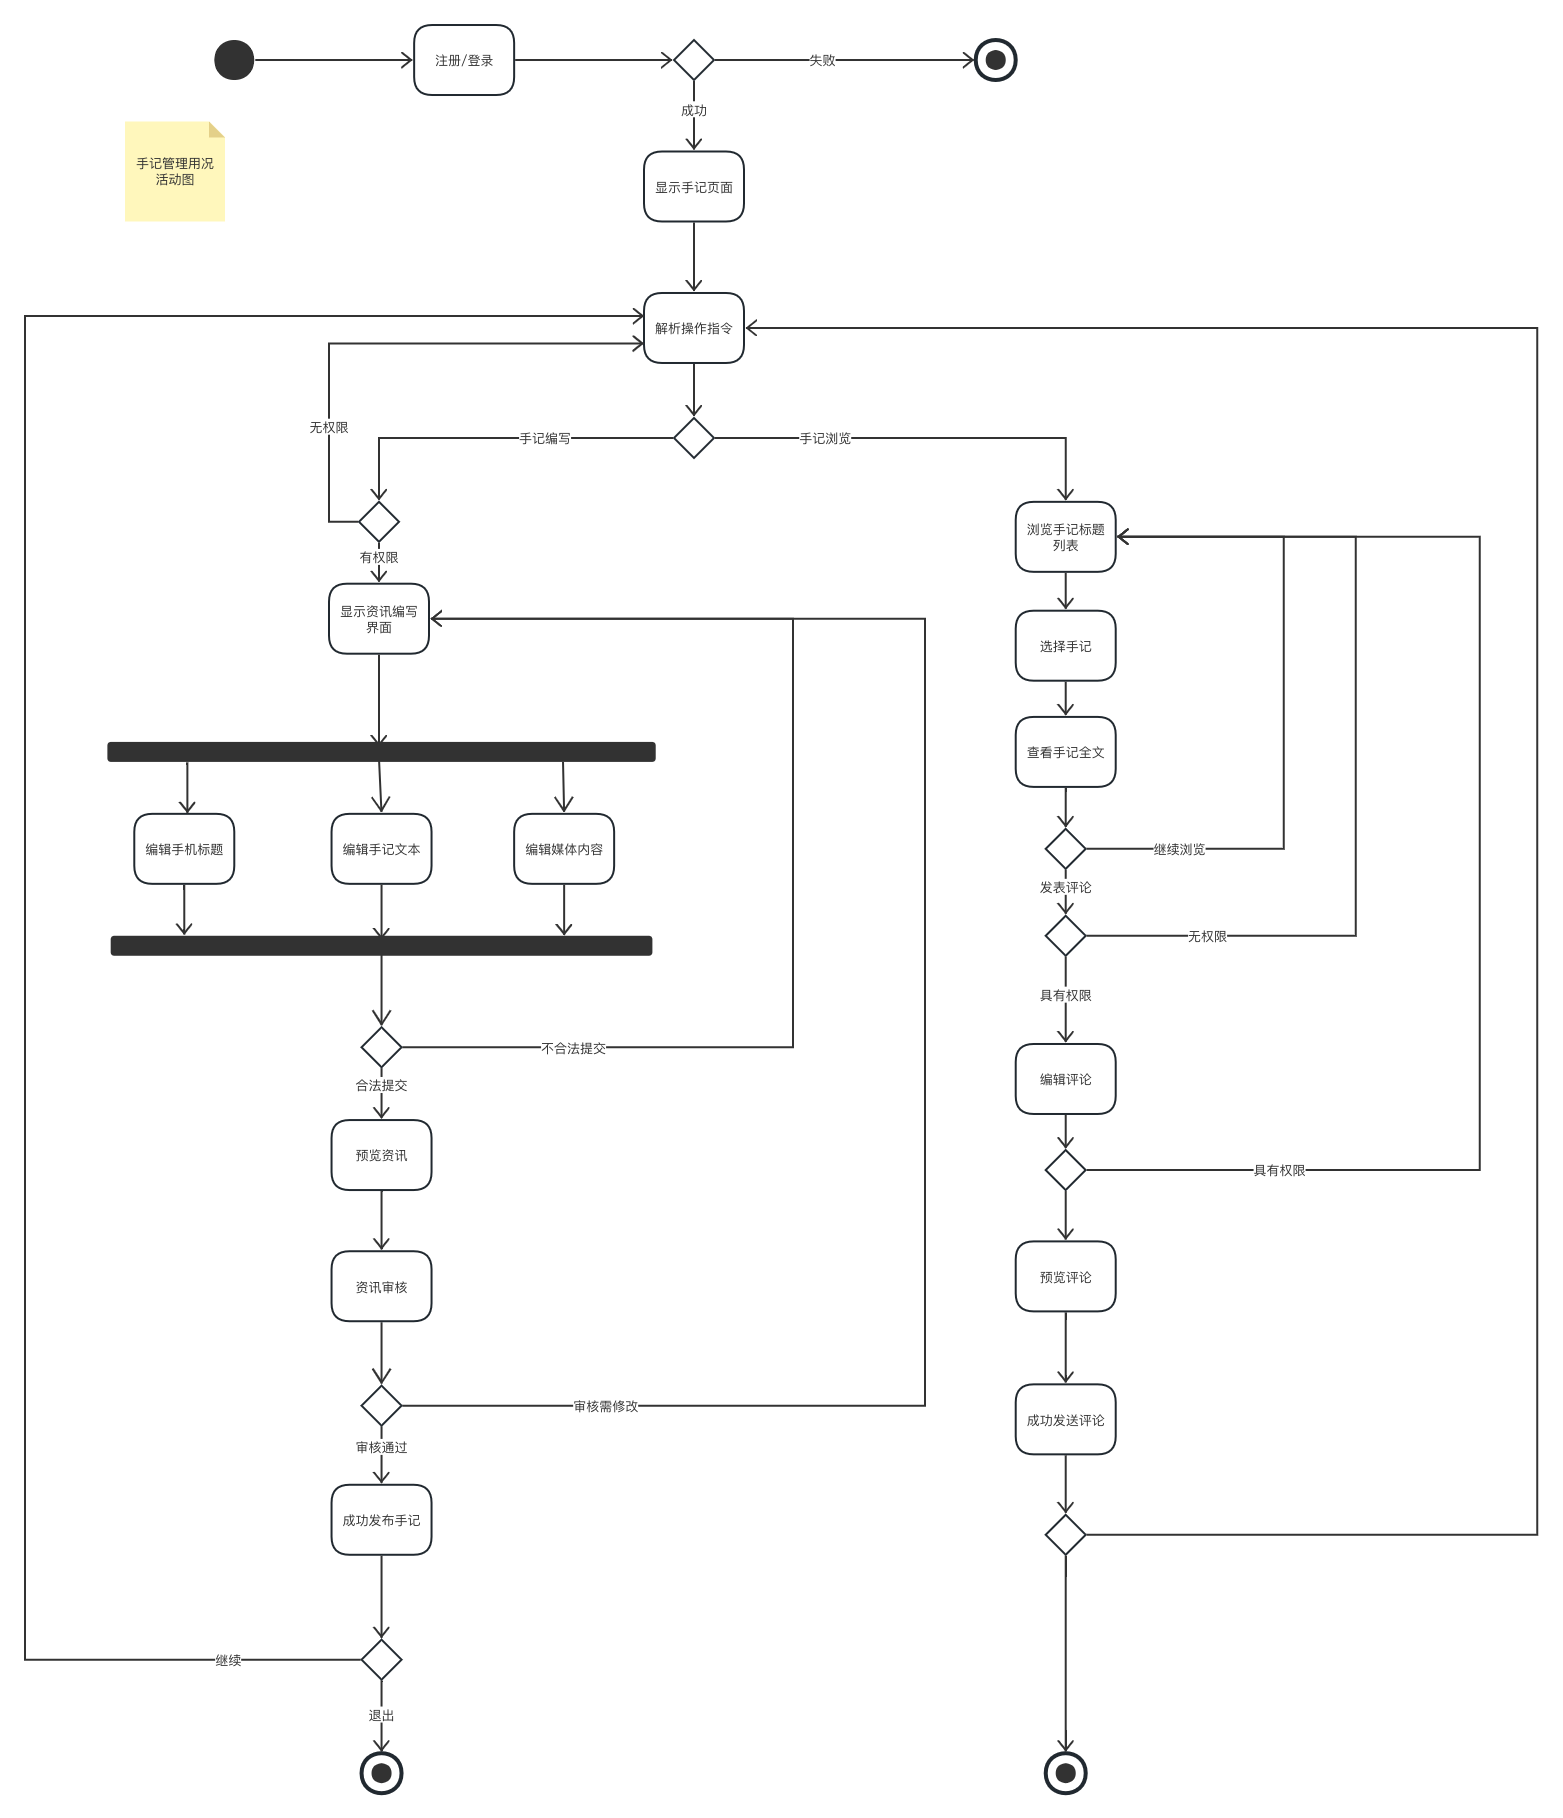
\includegraphics[scale=0.25]{OOA/fig/5-论坛管理/论坛管理用况活动图-2.png}} 
    \bicaption{Volunet交流论坛系统用况活动2子图}{Activity 2 Subgraph for Communication System Use Case of Volunet} 
\end{figure}

\begin{figure}[H] 
    \center{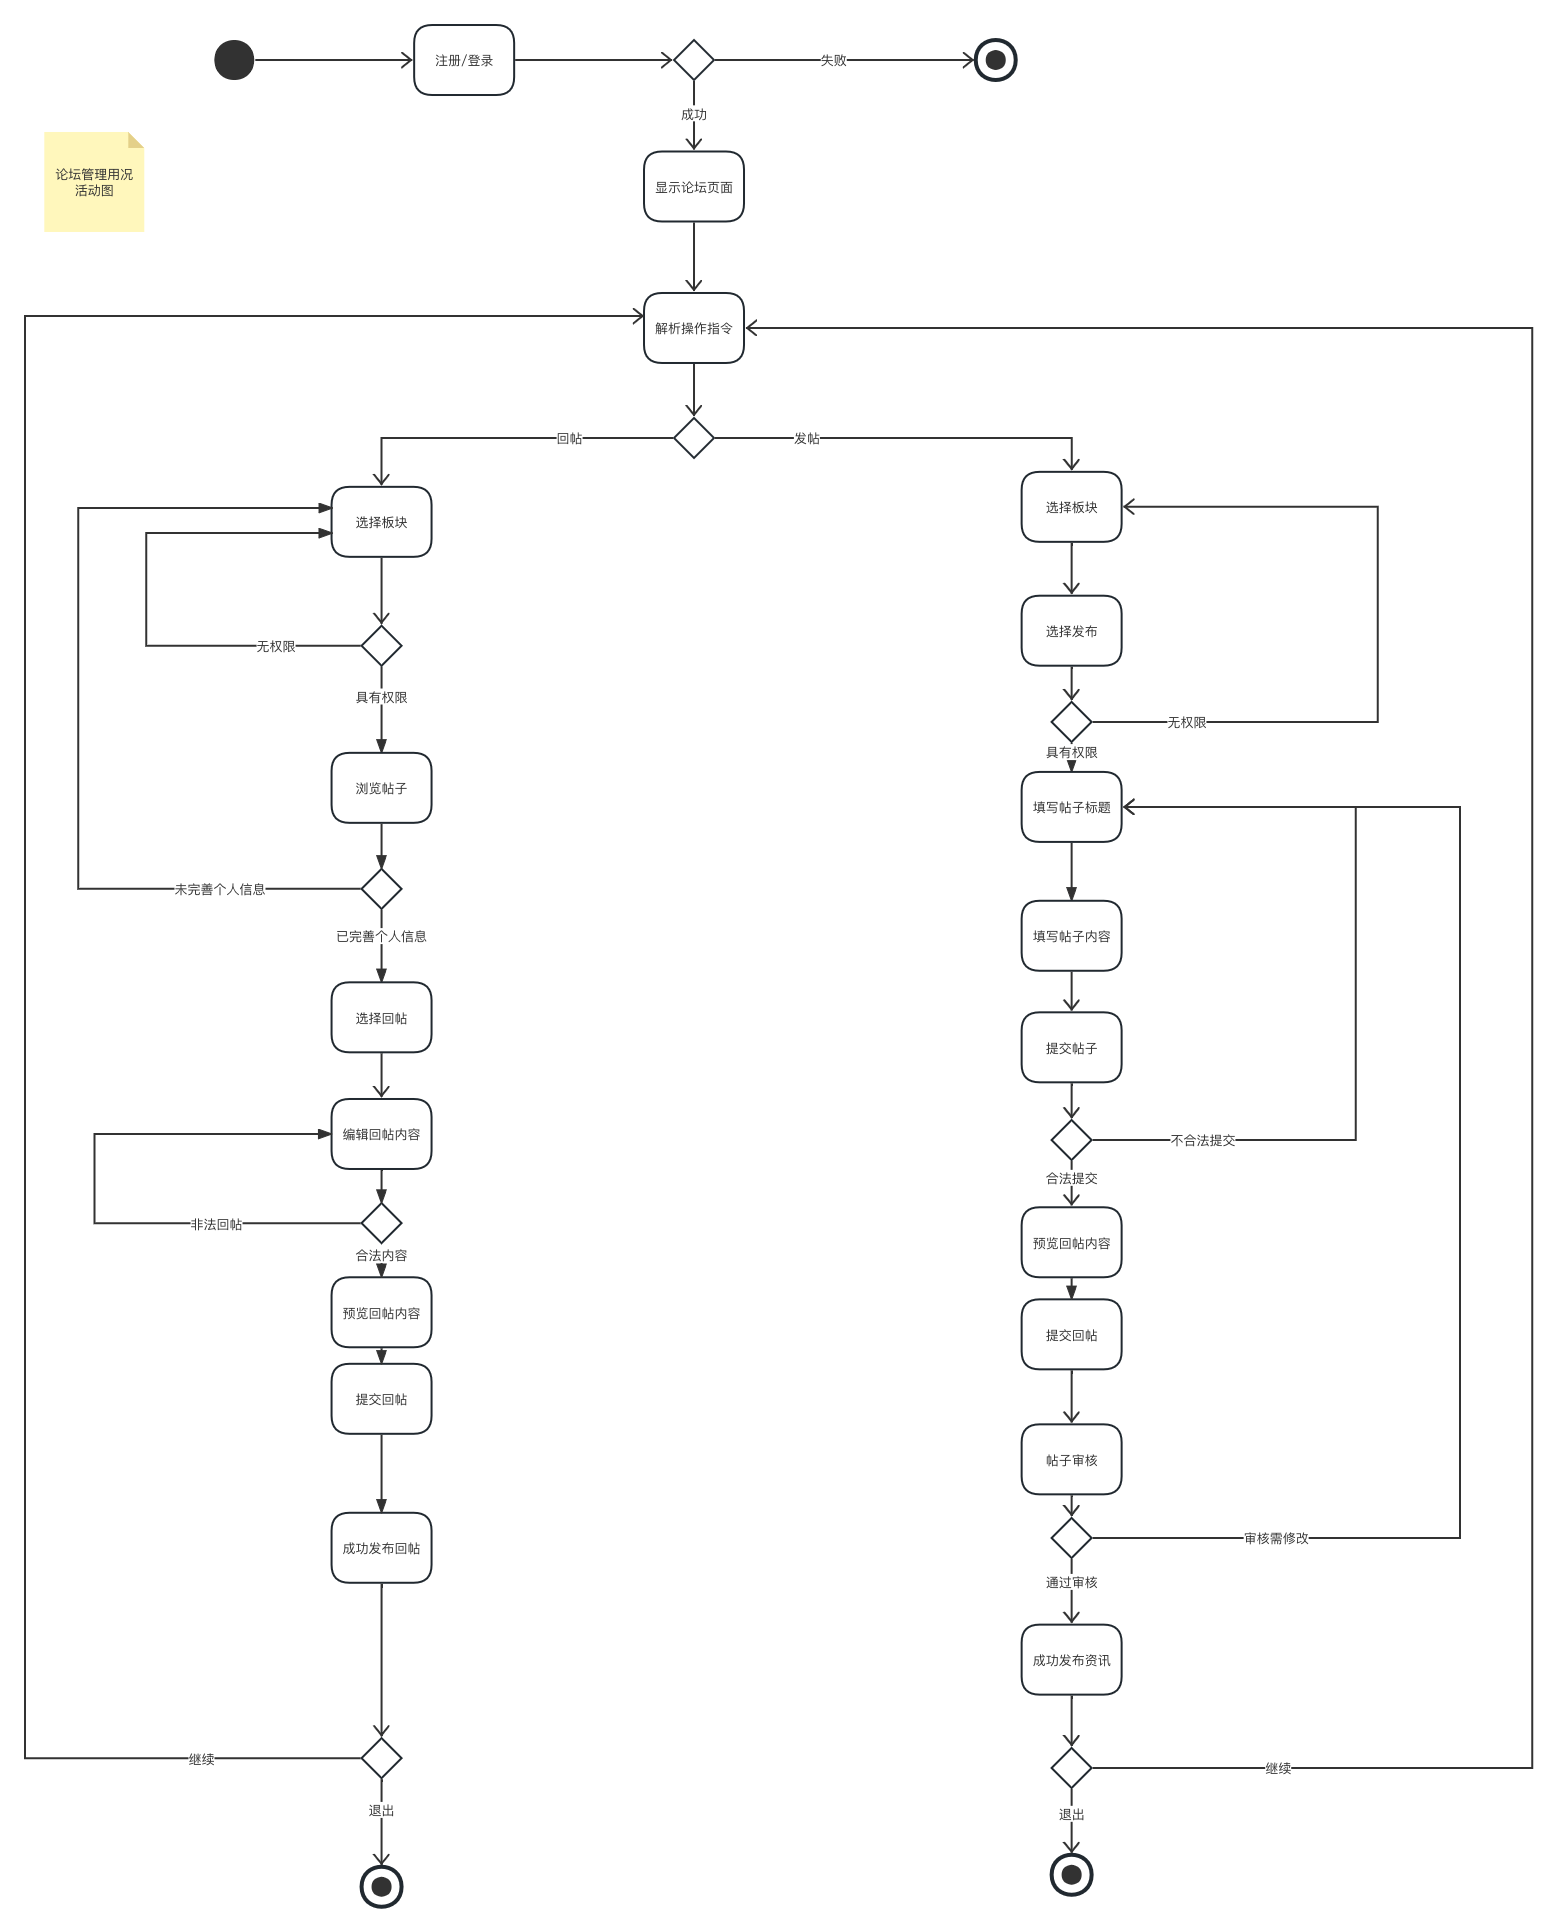
\includegraphics[scale=0.25]{OOA/fig/5-论坛管理/论坛管理用况活动图-3.png}} 
    \bicaption{Volunet交流论坛系统用况活动3子图}{Activity 3 Subgraph for Communication System Use Case of Volunet} 
\end{figure}

\begin{figure}[H] 
    \center{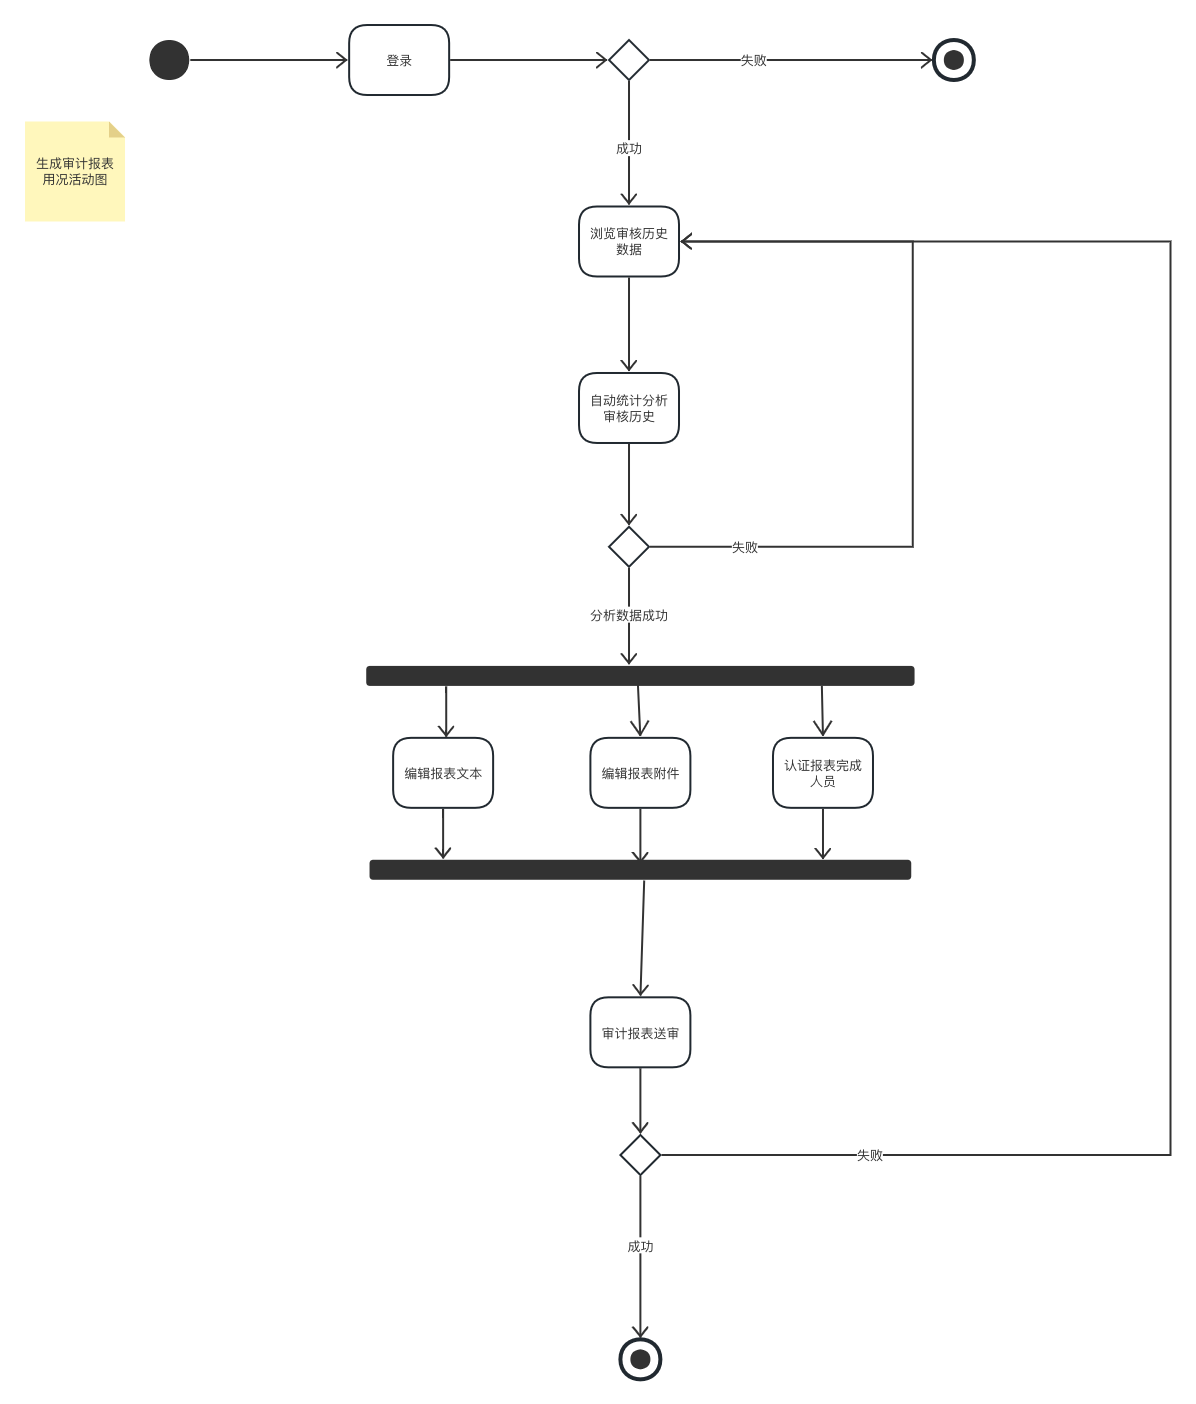
\includegraphics[scale=0.25]{OOA/fig/5-论坛管理/论坛管理用况活动图-4.png}} 
    \bicaption{Volunet交流论坛系统用况活动4子图}{Activity 4 Subgraph for Communication System Use Case of Volunet} 
\end{figure}

\subsubsection{志愿交友系统}
\begin{figure}[H] 
    \center{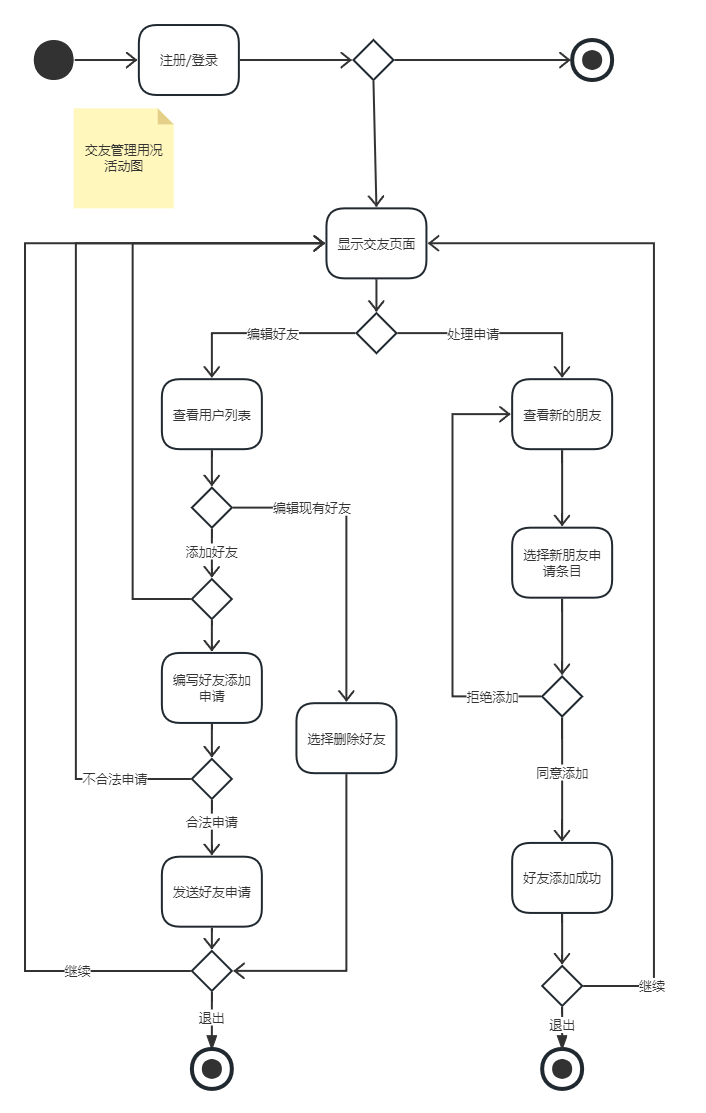
\includegraphics[scale=0.4]{OOA/fig/6-交友管理/志愿交友管理用况活动图.png}} 
    \bicaption{Volunet志愿交友系统用况活动1子图}{Activity 1 Subgraph for Volunteer Friends System Usage of Volunet} 
\end{figure}

\begin{figure}[H] 
    \center{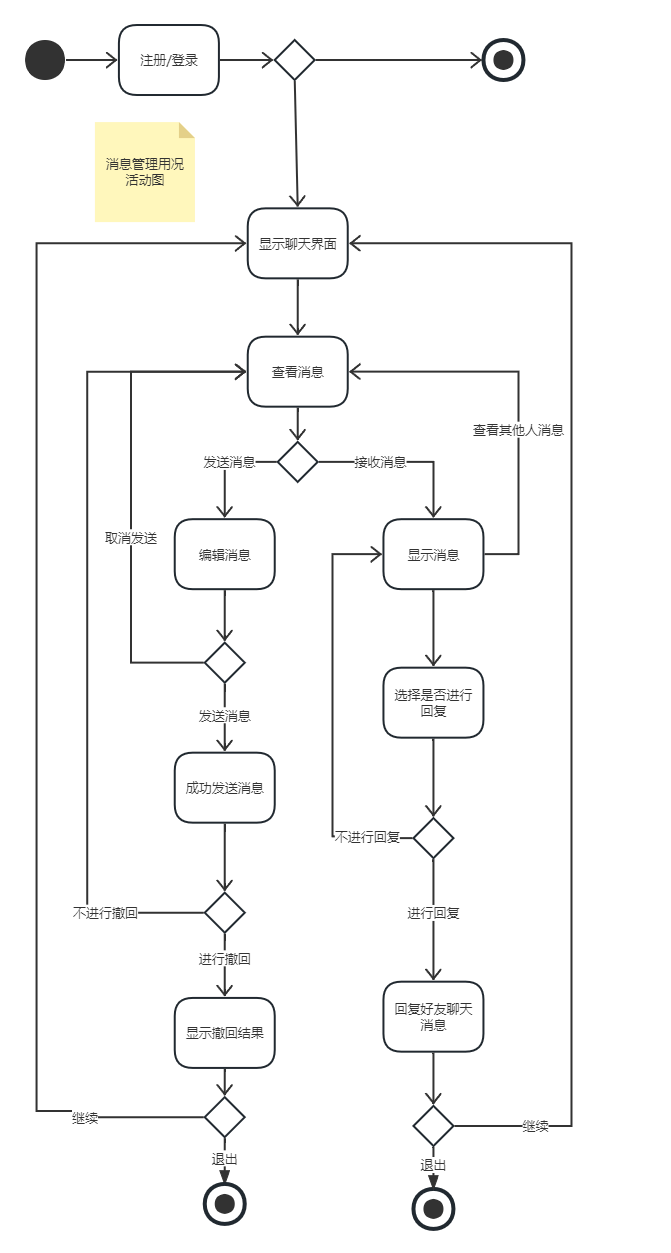
\includegraphics[scale=0.4]{OOA/fig/6-交友管理/志愿交友管理用况活动图 (1).png}} 
    \bicaption{Volunet志愿交友系统用况活动1子图}{Activity 1 Subgraph for Volunteer Friends System Usage of Volunet} 
\end{figure}














\newpage

\fancyhead[LH]{复旦大学软件工程}
\fancyhead[RH]{第五章\quad 静态建模}
\section{静态建模}






\subsection{类图}
\subsubsection{信息管理系统类图}
\begin{figure}[H] 
    \center{
\includegraphics[scale=0.56]{OOA/fig/1-信息管理/I-类图.pdf}} 
    \bicaption{Volunet信息管理系统类图}{Class Diagram for Information Management System of Volunet} 
\end{figure}

\subsubsection{志愿服务系统类图}
\begin{figure}[H] 
    \center{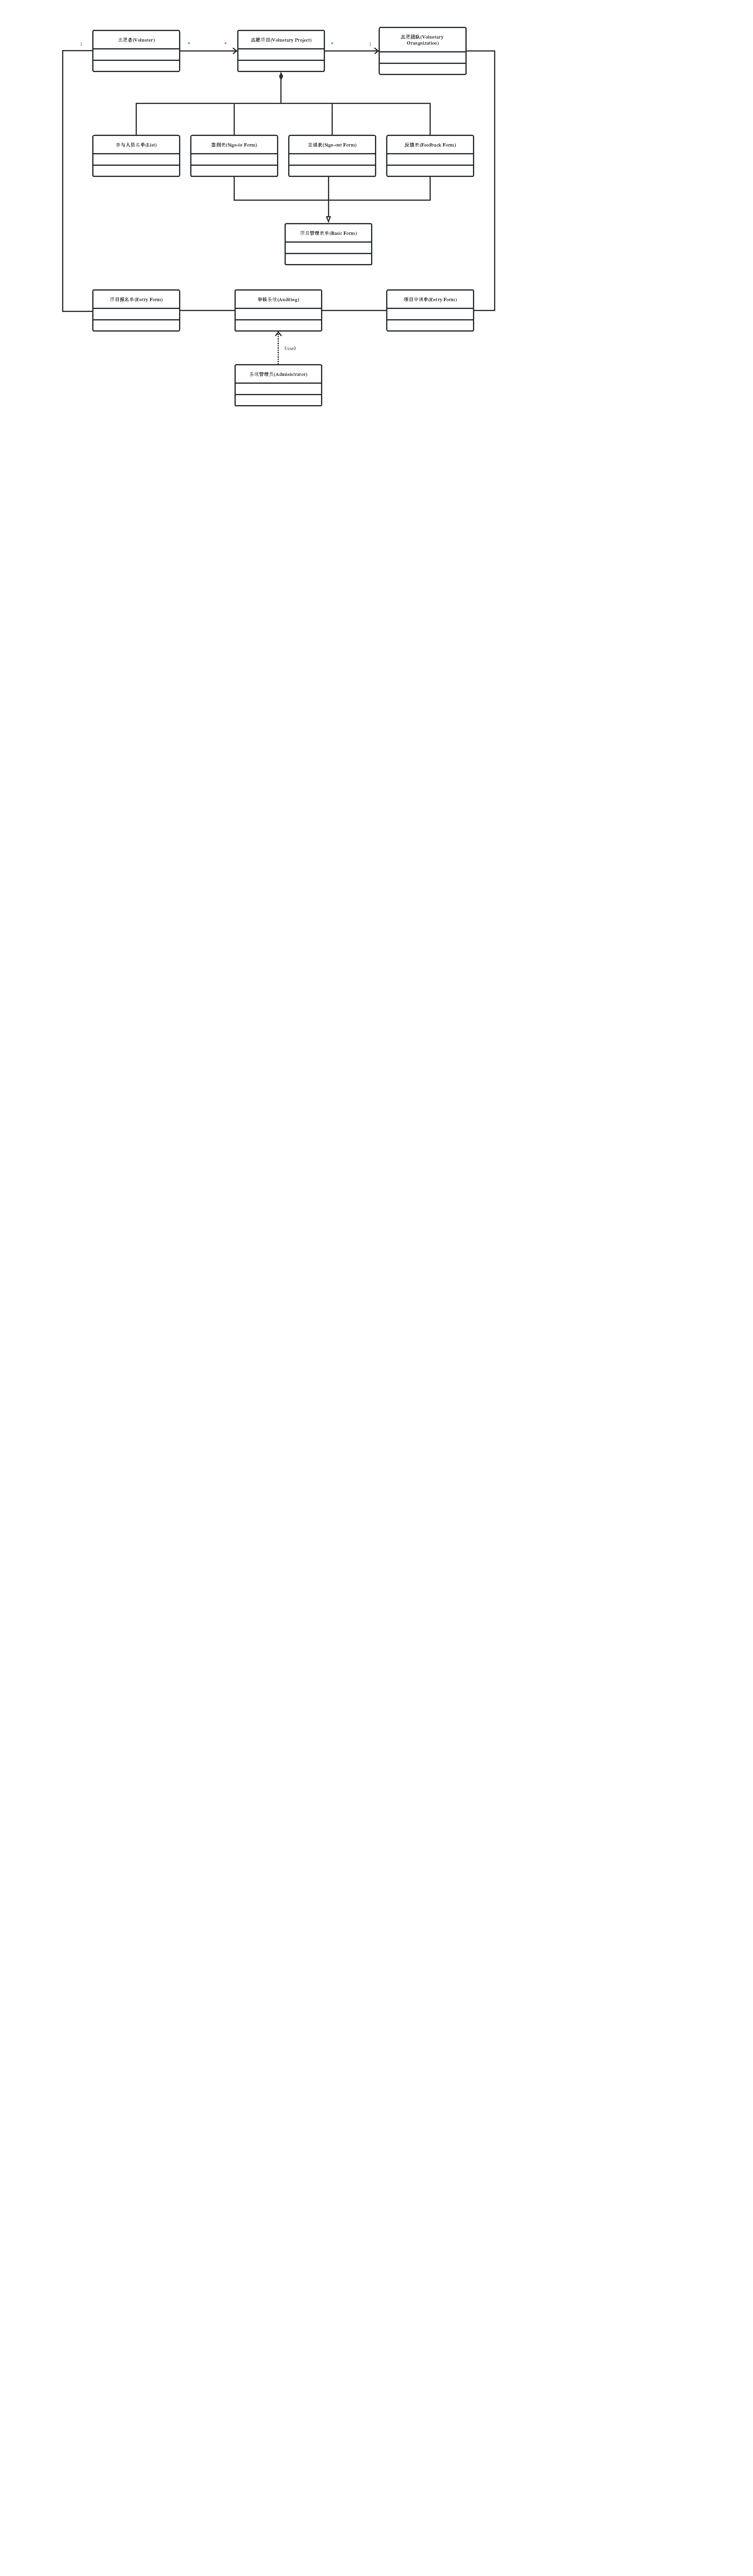
\includegraphics[scale=0.56]{OOA/fig/2-志愿服务/VS-类图.pdf}} 
    \bicaption{Volunet志愿服务系统类图}{Class Diagram for Voluntary Service System of Volunet} 
\end{figure}

\subsubsection{爱心捐助系统类图}
\begin{figure}[H] 
    \center{\includegraphics[scale=0.35]{OOA/fig/3-爱心管理/爱心管理类图-1.pdf}} 
    \bicaption{Volunet爱心捐助系统类图}{Class Diagram for Love Donation System of Volunet} 
\end{figure}

\subsubsection{公益课程系统类图}
\begin{figure}[H] 
    \center{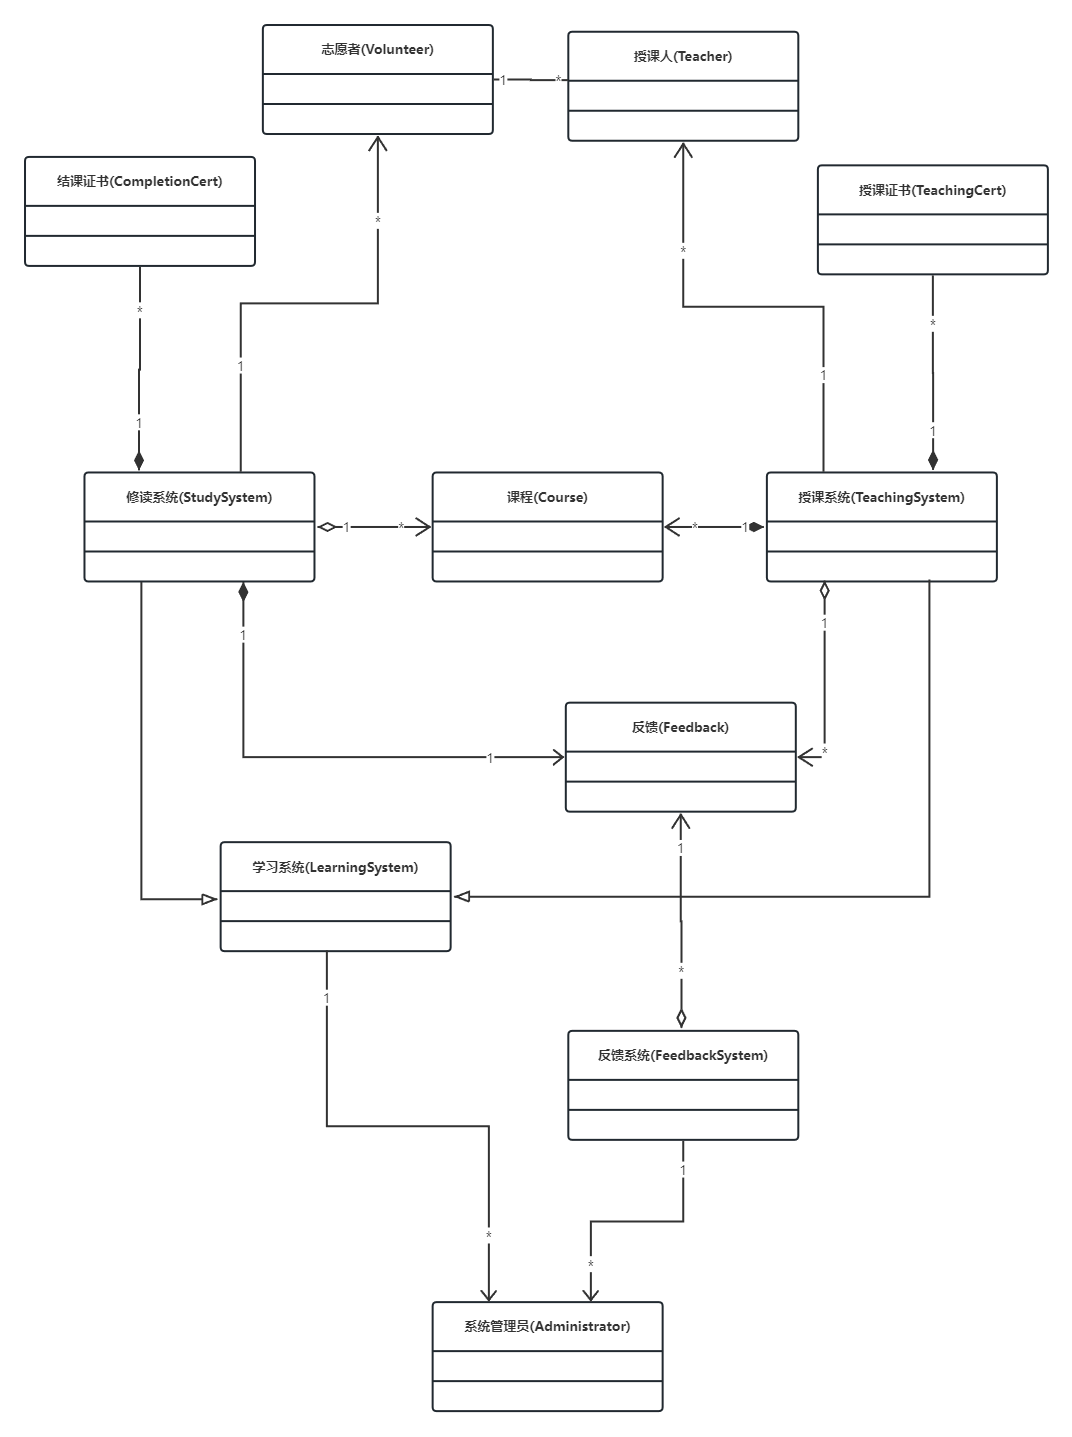
\includegraphics[scale=0.35]{OOA/fig/4-课程管理/课程管理类图.png}} 
    \bicaption{Volunet公益课程系统类图}{Class Diagram for Course System of Volunet} 
\end{figure}

\subsubsection{交流论坛系统类图}
\begin{figure}[H] 
    \center{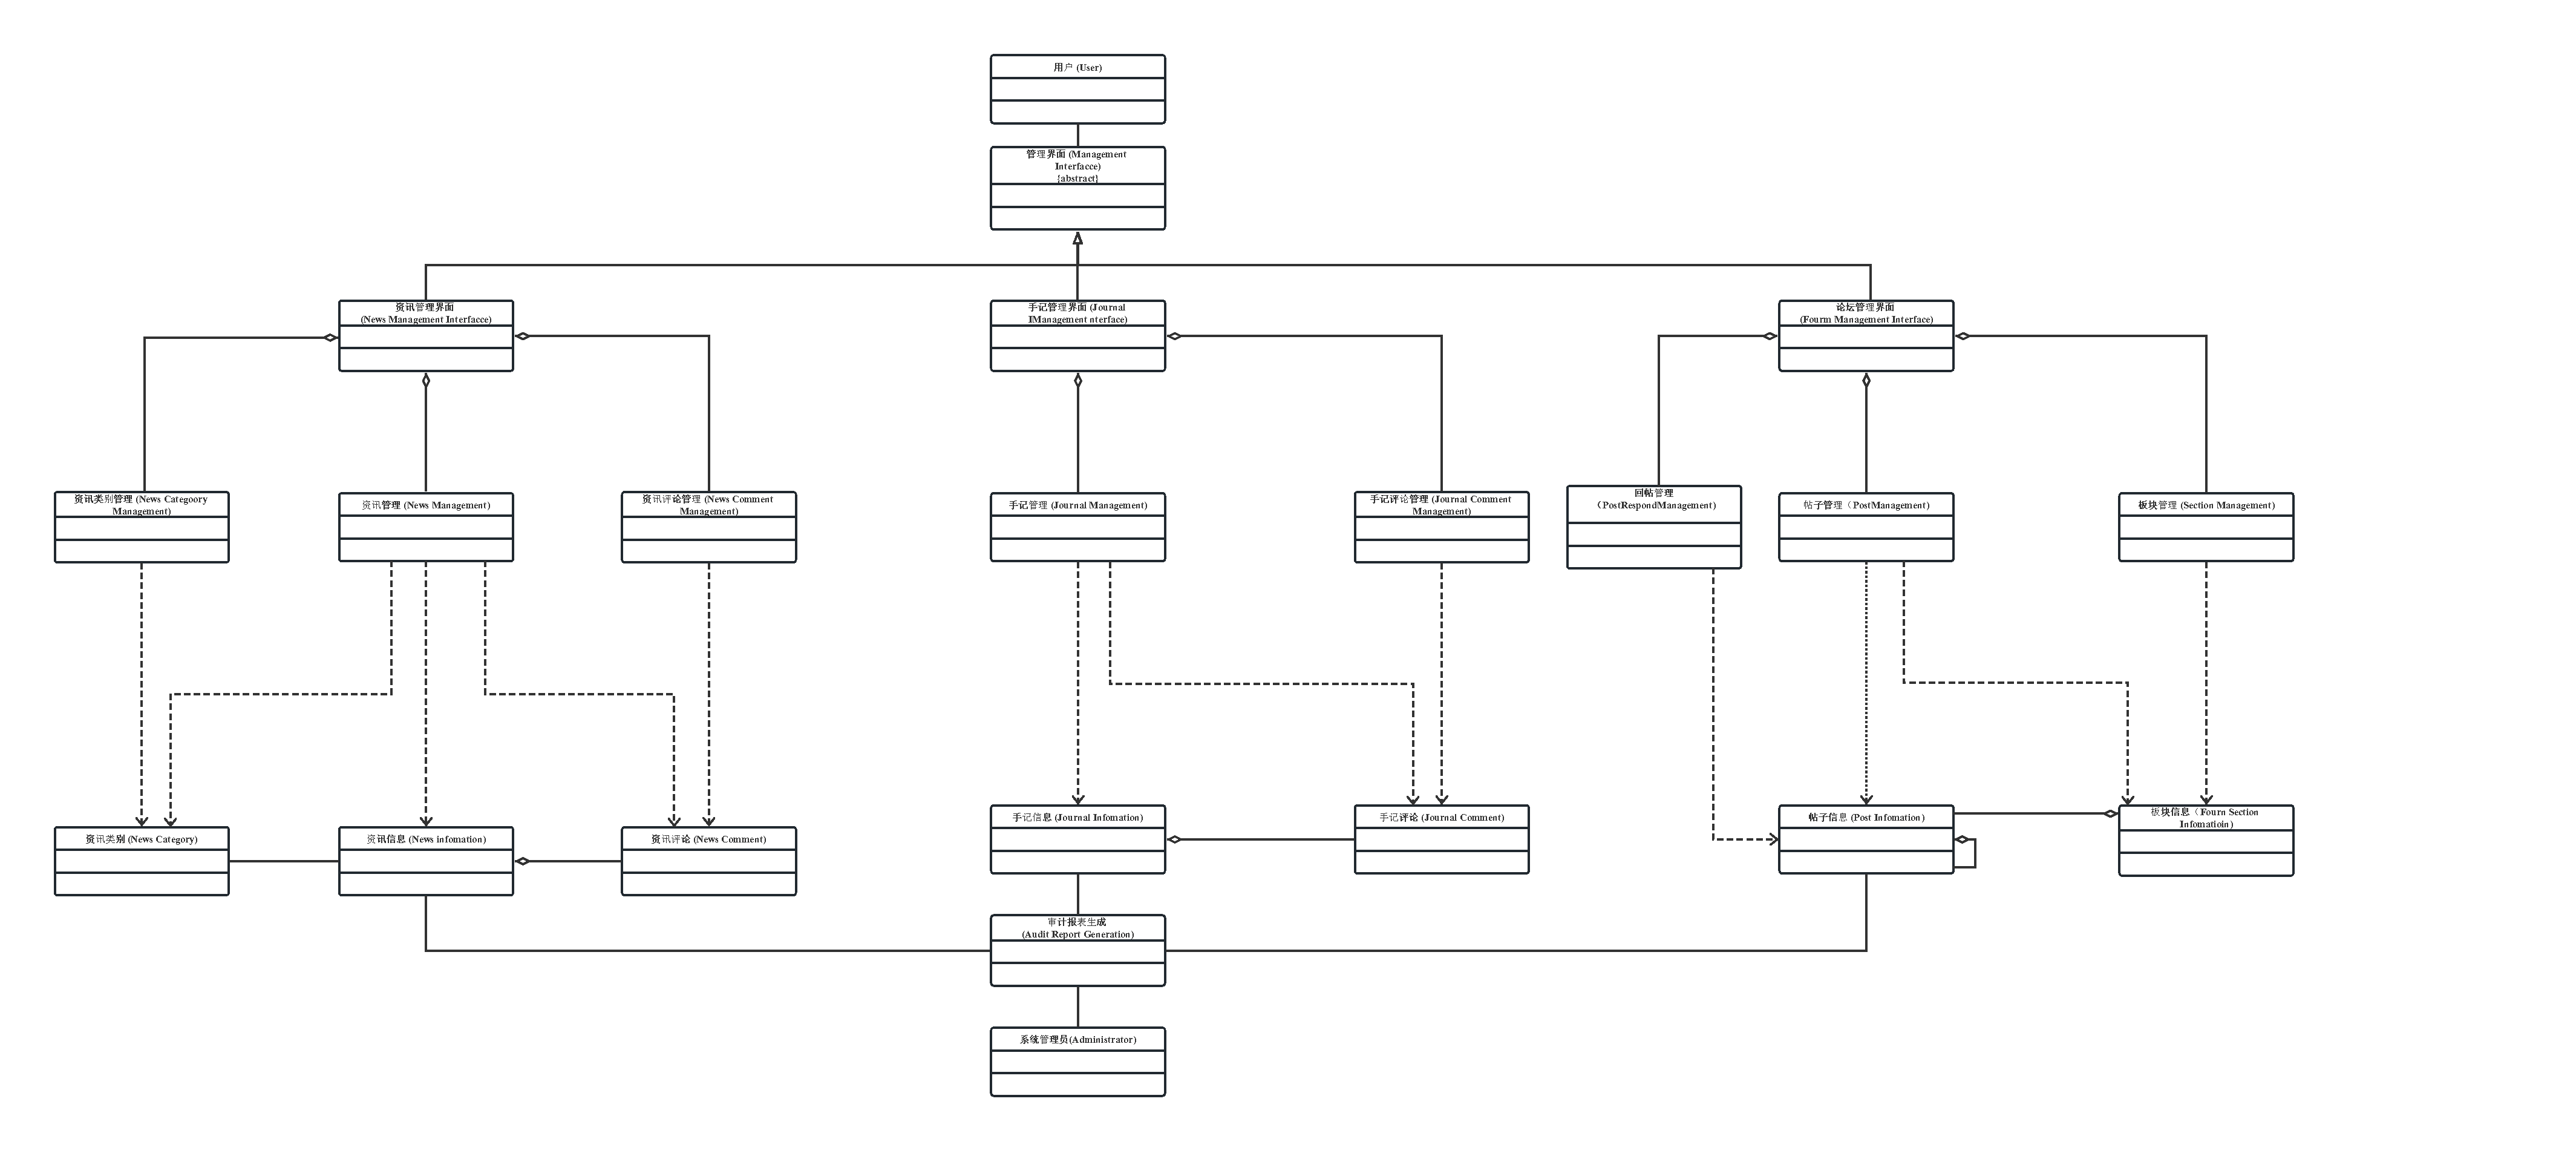
\includegraphics[scale=0.25, angle=90]{OOA/fig/5-论坛管理/论坛管理类图.pdf}} 
    \bicaption{Volunet交流论坛系统类图}{Class Diagram for Communication System of Volunet} 
\end{figure}

\subsubsection{志愿交友系统类图}
\begin{figure}[H] 
    \center{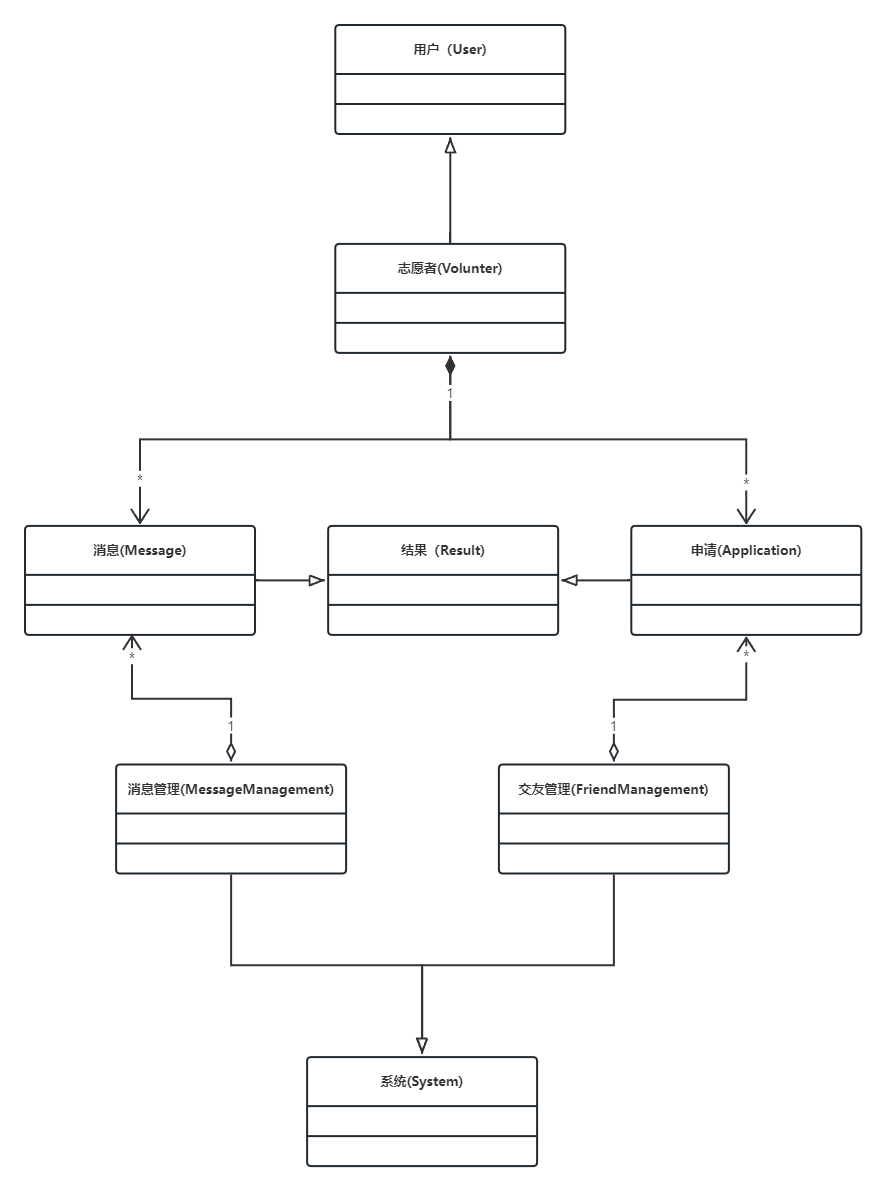
\includegraphics[scale=0.4]{OOA/fig/6-交友管理/志愿交友管理类图.png}} 
    \bicaption{Volunet志愿交友系统类图}{Class Diagram for Volunteer Friends System of Volunet} 
\end{figure}


\subsection{类的属性和操作}

\subsubsection{信息管理系统}

\paragraph{信息管理系统类属性与操作图}~{}
\begin{figure}[H] 
    \center{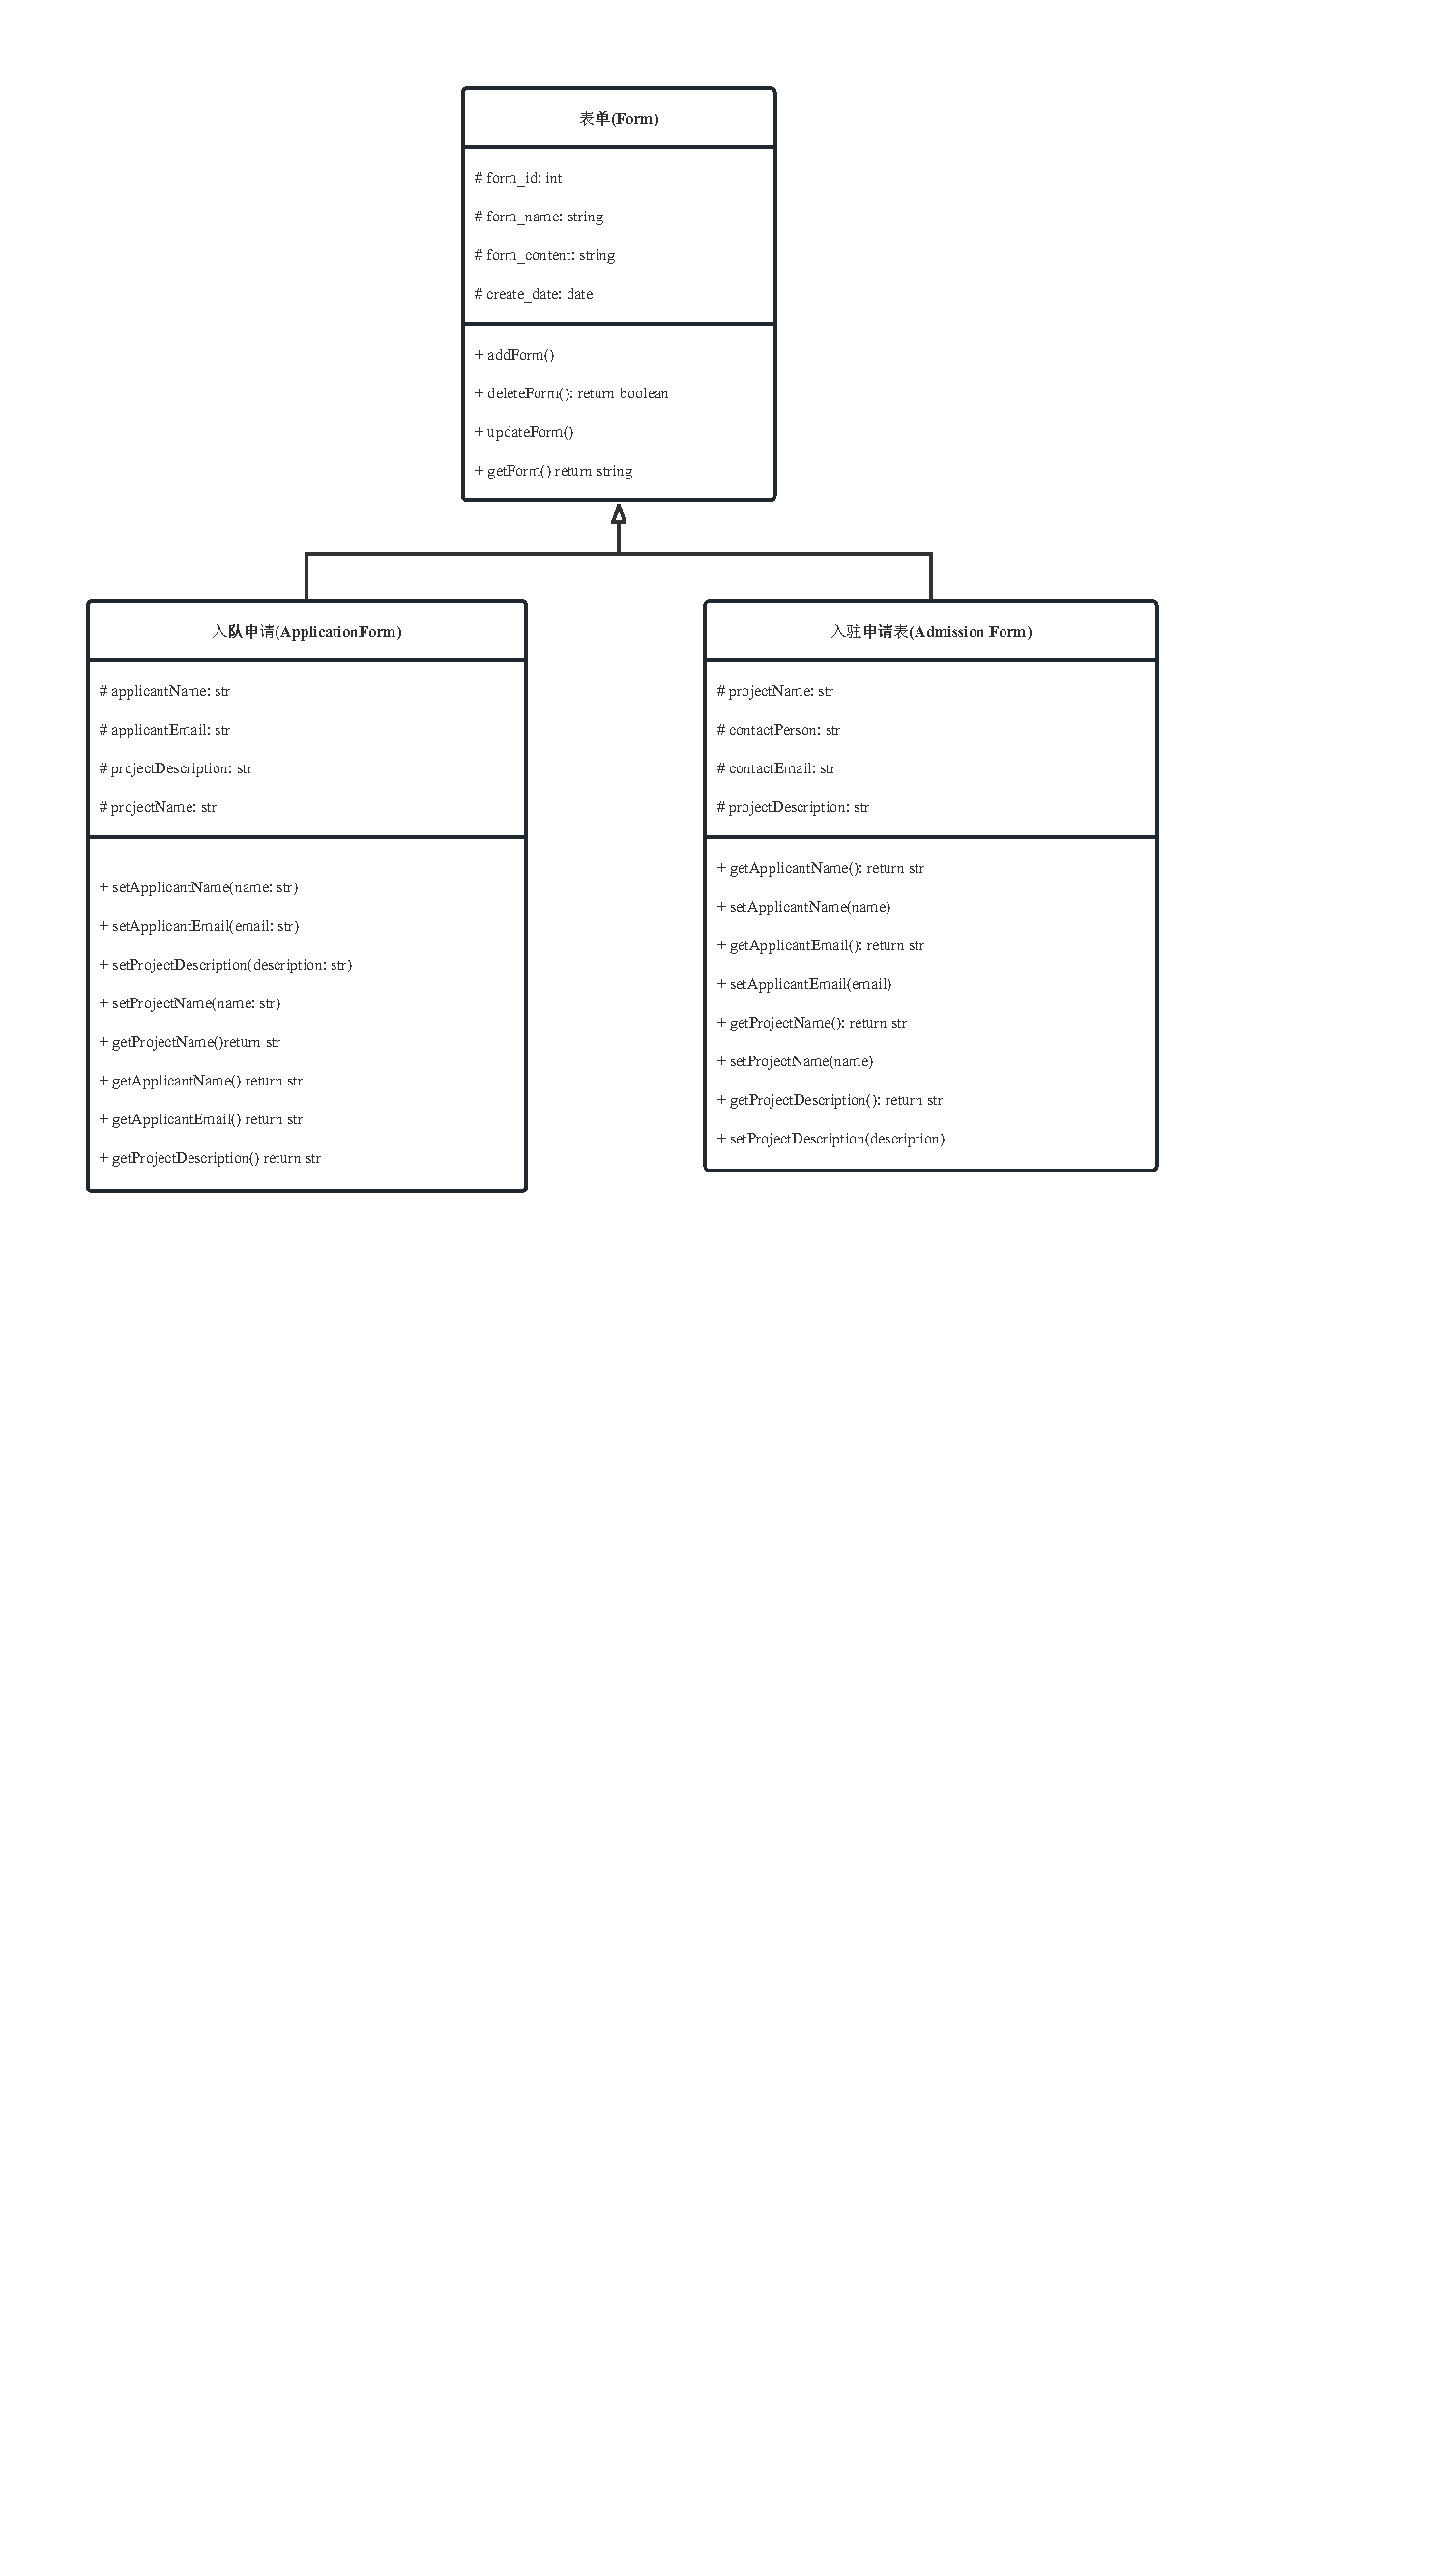
\includegraphics[scale=0.7]{OOA/fig/1-信息管理/信息管理类图-1.pdf}} 
    \bicaption{Volunet信息管理系统类属性与操作1子图}{Class Attributes and Operations Sub-Diagram 1 for Information Management System of Volunet} 
\end{figure}

\begin{figure}[H] 
    \center{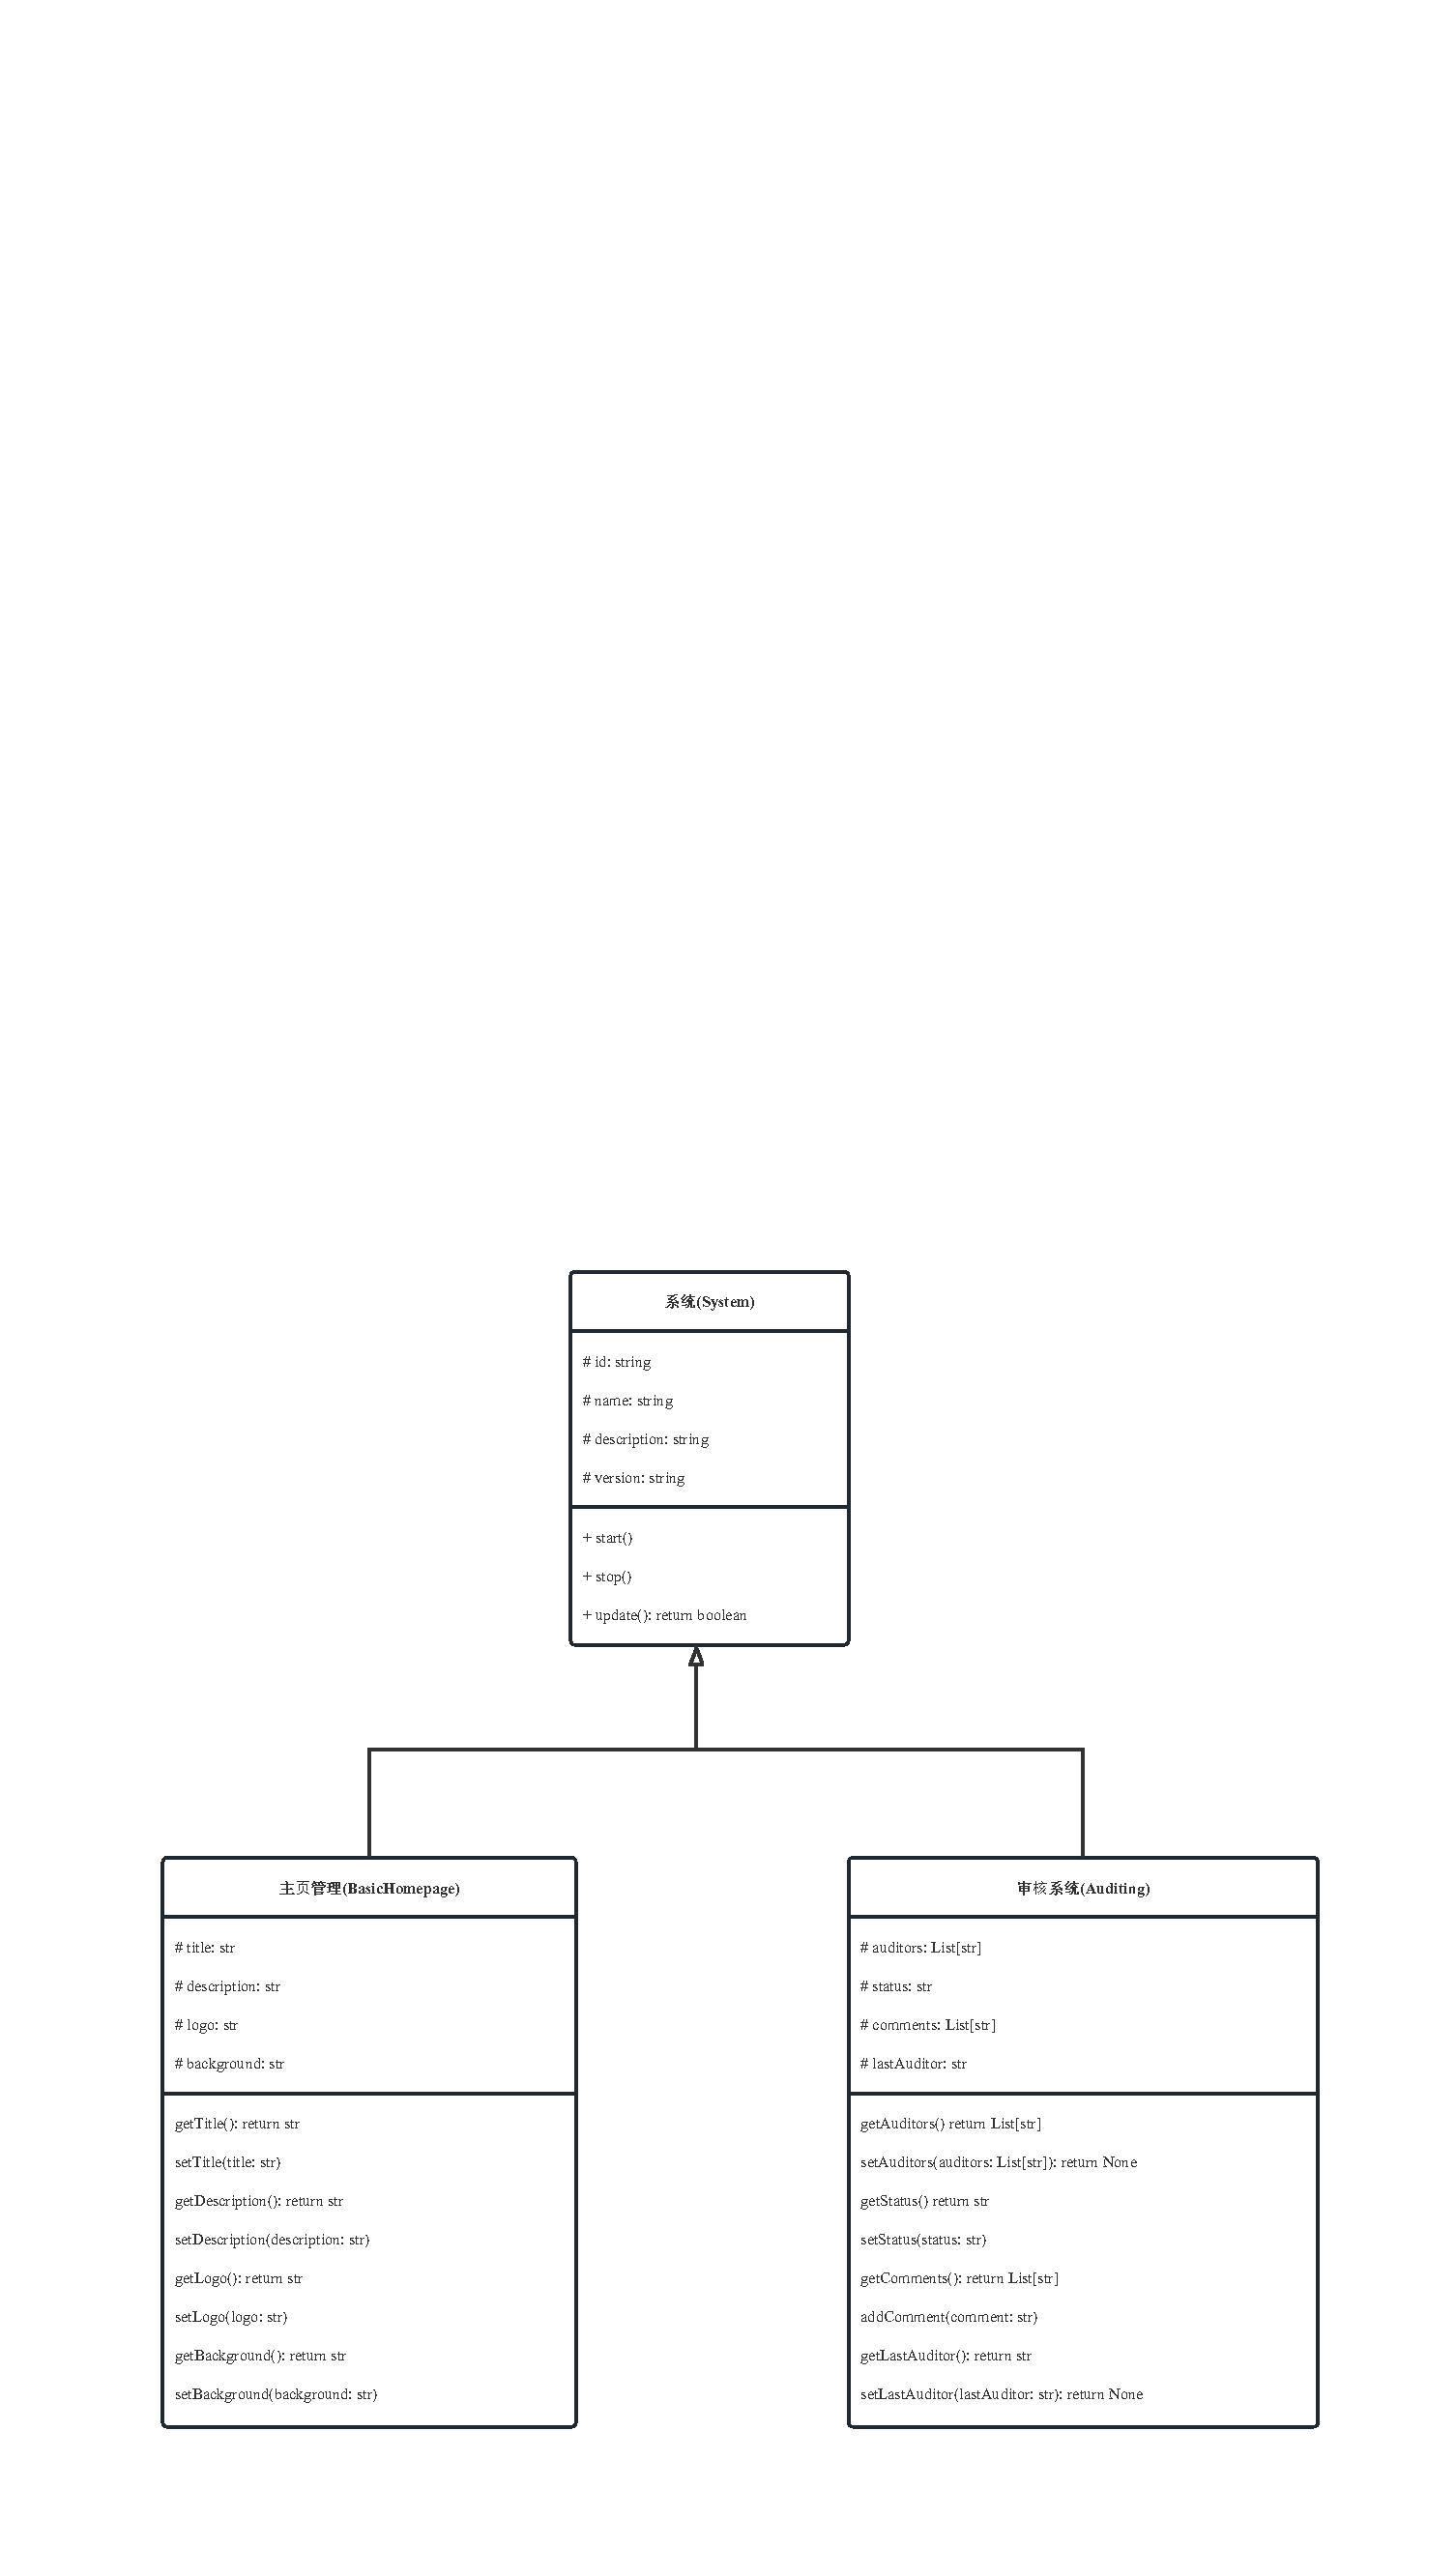
\includegraphics[scale=0.7]{OOA/fig/1-信息管理/信息管理类图-2.pdf}} 
    \bicaption{Volunet爱心捐助系统类属性与操作2子图}{Class Attributes and Operations Sub-Diagram 2 for Information Management System of Volunet} 
\end{figure}

\paragraph{信息管理系统类属性与操作描述}~{}

信息管理系统中类包含表单、入队申请、入驻申请表、系统、主页管理、审核系统,它们的属性与操作描述如下:

% 表单、入队申请、入驻申请表、系统、主页管理、审核系统
\begin{table}[H]  
\caption{“表单”类词条描述}  
\begin{center}  
    \begin{tabular}{l p{11cm}} 
        \hline
        \quad 名称:  &  表单 \\
        \hline
        \quad 编号:  & 1.1 \\
        \hline
        \quad 英文:  &  Form \\
        \hline
        \quad 简述:  & 用于收集、记录和处理信息的文档或工具 \\
        \hline
        \quad 属性:  & form\_id、form\_name、form\_content、create\_date: date\\
        \hline
        \quad 操作:  & addForm()、deleteForm()、updateForm()、getForm()\\
        \hline
        \quad 相关类:  & 入队申请、入驻申请表 \\
        \hline
    \end{tabular}
\end{center}
\end{table}

\begin{table}[H]  
\caption{“入队申请”类词条描述}  
\begin{center}  
    \begin{tabular}{l p{11cm}} 
        \hline
        \quad 名称:  &  入队申请 \\
        \hline
        \quad 编号:  & 1.2 \\
        \hline
        \quad 英文:  & ApplicationForm\\
        \hline
        \quad 简述:  & 用于申请加入某个志愿团队的表单 \\
        \hline
        \quad 属性:  & # applicantName、applicantEmail、projectDescription、projectName\\
        \hline
        \quad 操作:  & setApplicantName()、setApplicantEmail()、setProjectDescription()、 setProjectName()、getProjectName()、getApplicantName()、getApplicantEmail()、getProjectDescription()\\
        \hline
        \quad 相关类:  & 表单、志愿者。审核系统 \\
        \hline
    \end{tabular}
\end{center}
\end{table}

\begin{table}[H]  
\caption{“入驻申请表”类词条描述}  
\begin{center}  
    \begin{tabular}{l p{11cm}} 
        \hline
        \quad 名称:  &  入驻申请表 \\
        \hline
        \quad 编号:  & 1.3 \\
        \hline
        \quad 英文:  &  AdmissionForm \\
        \hline
        \quad 简述:  & 用于志愿团队申请入驻的表单 \\
        \hline
        \quad 属性:  & projectName、contactPerson、contactEmail、projectDescription\\
        \hline
        \quad 操作:  & + getApplicantName()、setApplicantName()、getApplicantEmail()、setApplicantEmail()、getProjectName()、setProjectName()、getProjectDescription()、setProjectDescription
\\
        \hline
        \quad 相关类:  & 表单、志愿团队、审核系统 \\
        \hline
    \end{tabular}
\end{center}
\end{table}

\begin{table}[H]  
\caption{“系统”类词条描述}  
\begin{center}  
    \begin{tabular}{l p{11cm}} 
        \hline
        \quad 名称:  &  系统 \\
        \hline
        \quad 编号:  & 1.4 \\
        \hline
        \quad 英文:  &  System \\
        \hline
        \quad 简述:  & 信息管理系统的简称 \\
        \hline
        \quad 属性:  & id、name、description、version\\
        \hline
        \quad 操作:  & start()、stop()、update()\\
        \hline
        \quad 相关类:  & 主页管理、审核系统 \\
        \hline
    \end{tabular}
\end{center}
\end{table}

\begin{table}[H]  
\caption{“主页管理”类词条描述}  
\begin{center}  
    \begin{tabular}{l p{11cm}} 
        \hline
        \quad 名称:  &  主页管理 \\
        \hline
        \quad 编号:  & 1.5 \\
        \hline
        \quad 英文:  &  BasicHomepage \\
        \hline
        \quad 简述:  & 负责对志愿者主页进行管理的系统 \\
        \hline
        \quad 属性:  & title、description、logo、background\\
        \hline
        \quad 操作:  & getTitle()、setTitle()、getDescription()、setDescription()、getLogo()、setLogo()、getBackground()、setBackground()\\
        \hline
        \quad 相关类:  & 系统、志愿者 \\
        \hline
    \end{tabular}
\end{center}
\end{table}

\begin{table}[H]  
\caption{“审核系统”类词条描述}  
\begin{center}  
    \begin{tabular}{l p{11cm}} 
        \hline
        \quad 名称:  &  审核系统 \\
        \hline
        \quad 编号:  & 1.6 \\
        \hline
        \quad 英文:  &  Auditing \\
        \hline
        \quad 简述:  & 负责信息审核的系统 \\
        \hline
        \quad 属性:  & auditors、status、comments、lastAuditor\\
        \hline
        \quad 操作:  & getAuditors()、setAuditors()、getStatus()、setStatus()、getComments()、addComment()、getLastAuditor()、setLastAuditor()
\\
        \hline
        \quad 相关类:  & 系统、系统管理员 \\
        \hline
    \end{tabular}
\end{center}
\end{table}

\subsubsection{志愿服务系统}

\paragraph{志愿服务系统类属性与操作图}~{}
\begin{figure}[H] 
    \center{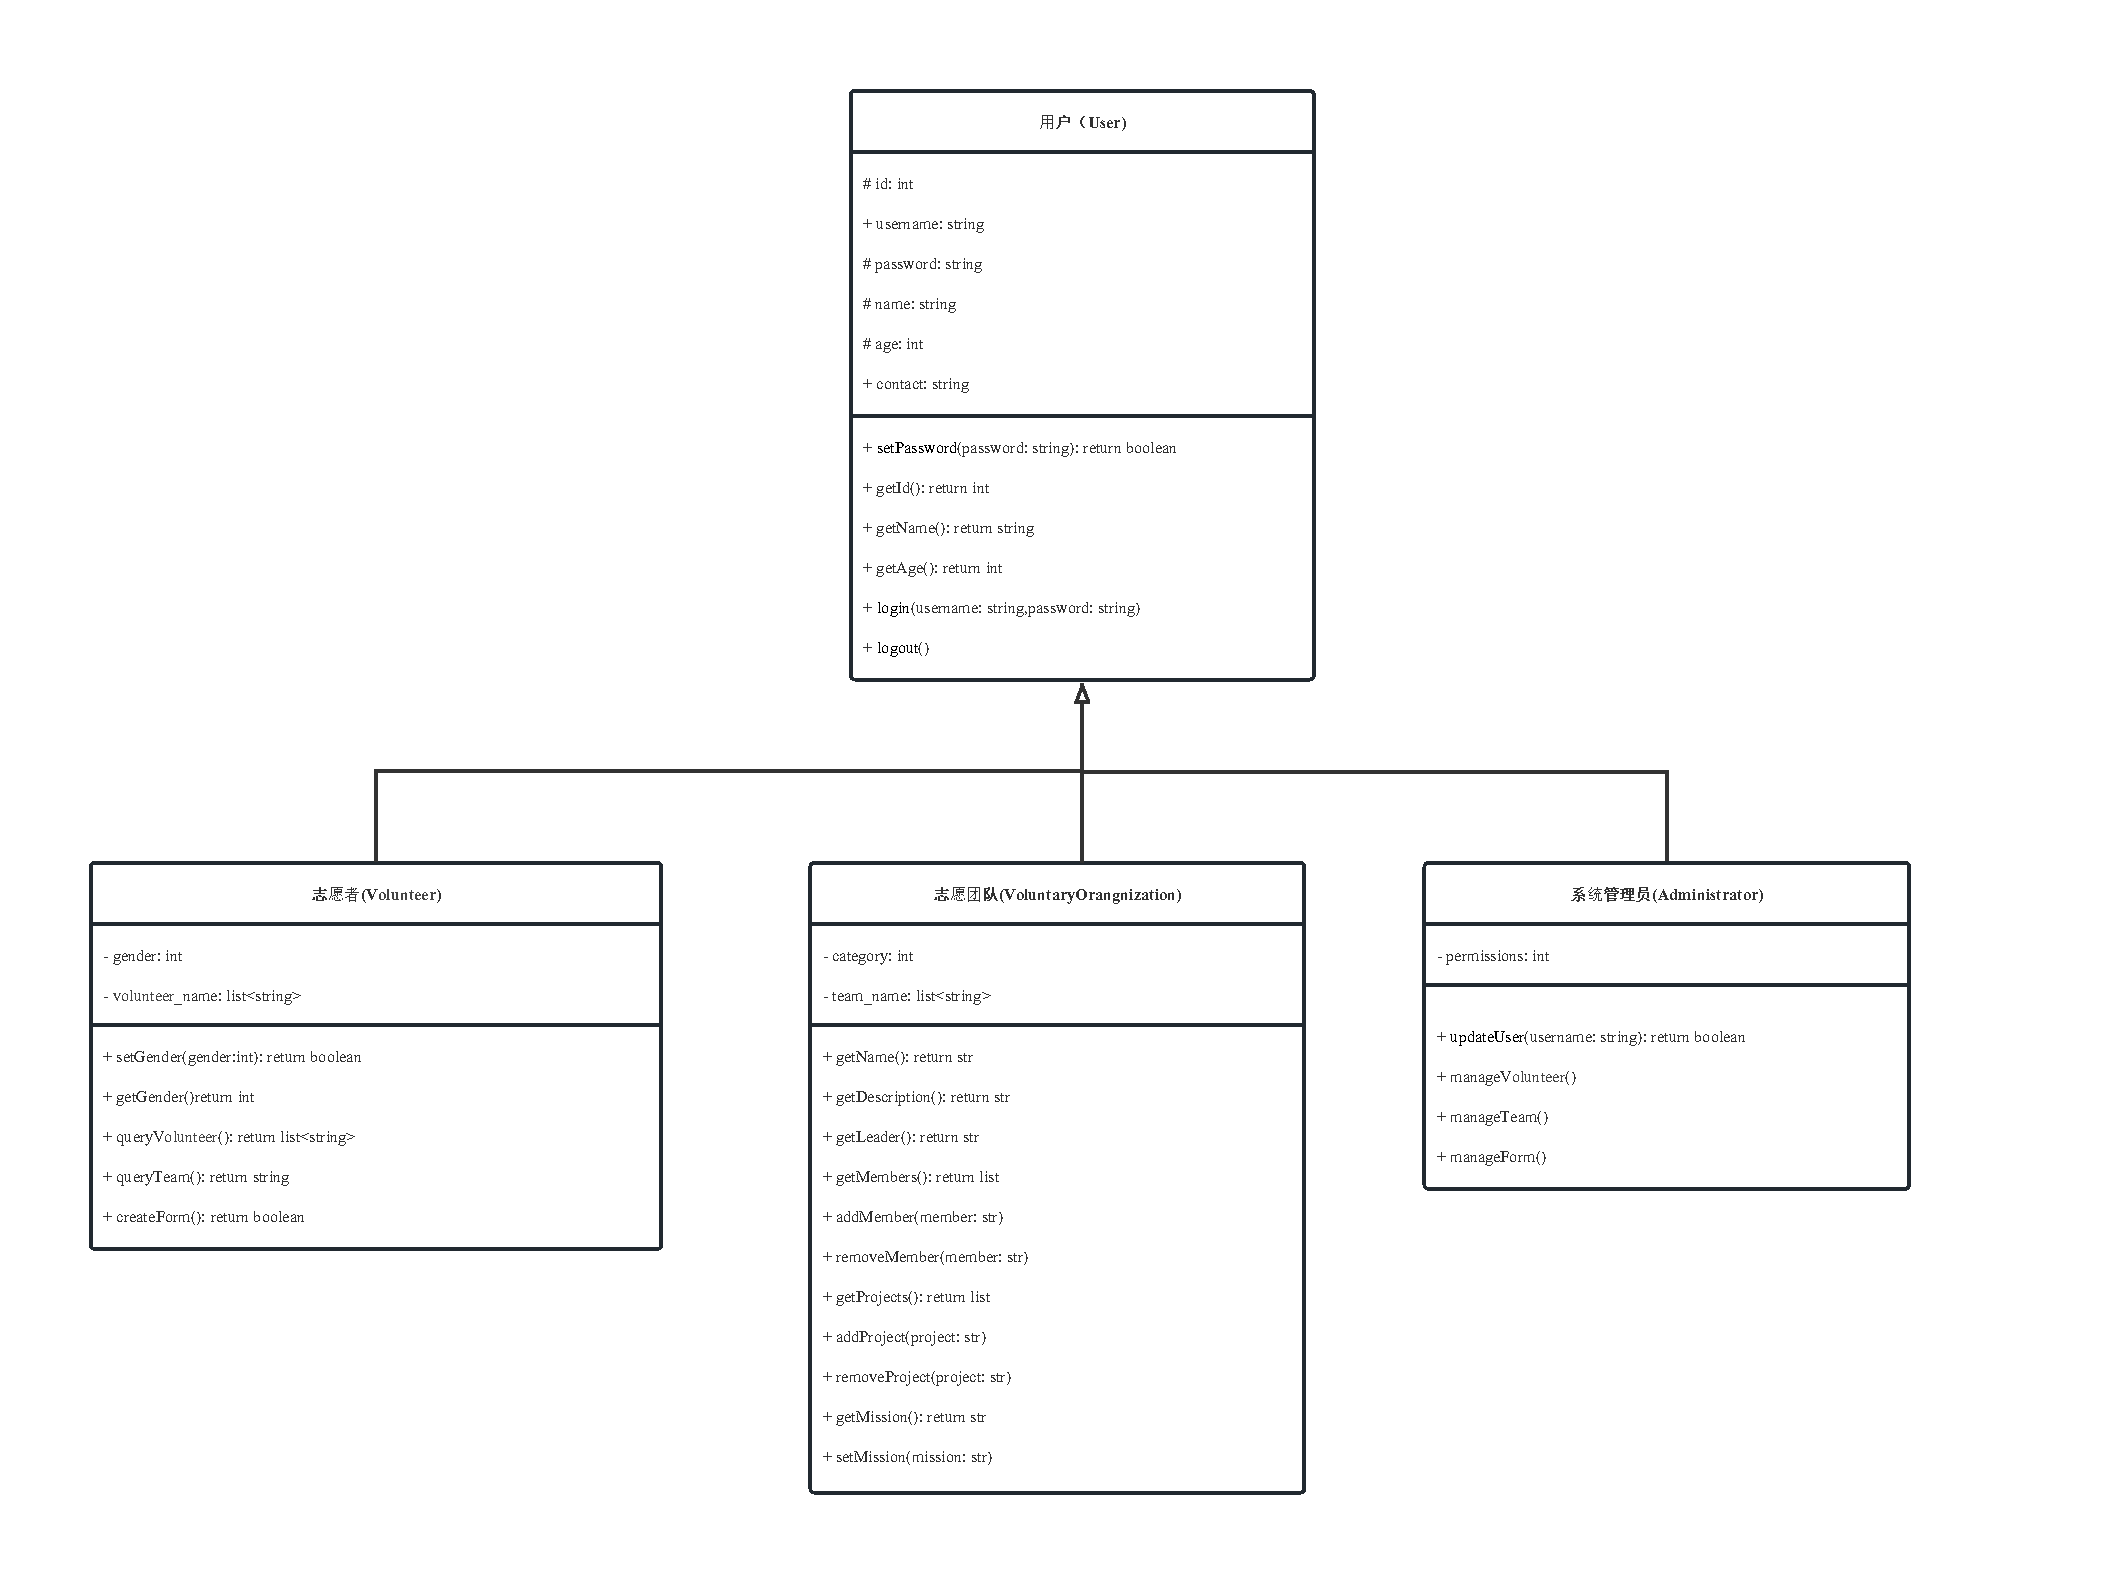
\includegraphics[scale=0.5]{OOA/fig/2-志愿服务/志愿服务类图-1.pdf}} 
    \bicaption{Volunet志愿服务系统类属性与操作1子图}{Class Attributes and Operations Sub-Diagram 1 for Volunteer Service System of Volunet} 
\end{figure}

\begin{figure}[H] 
    \center{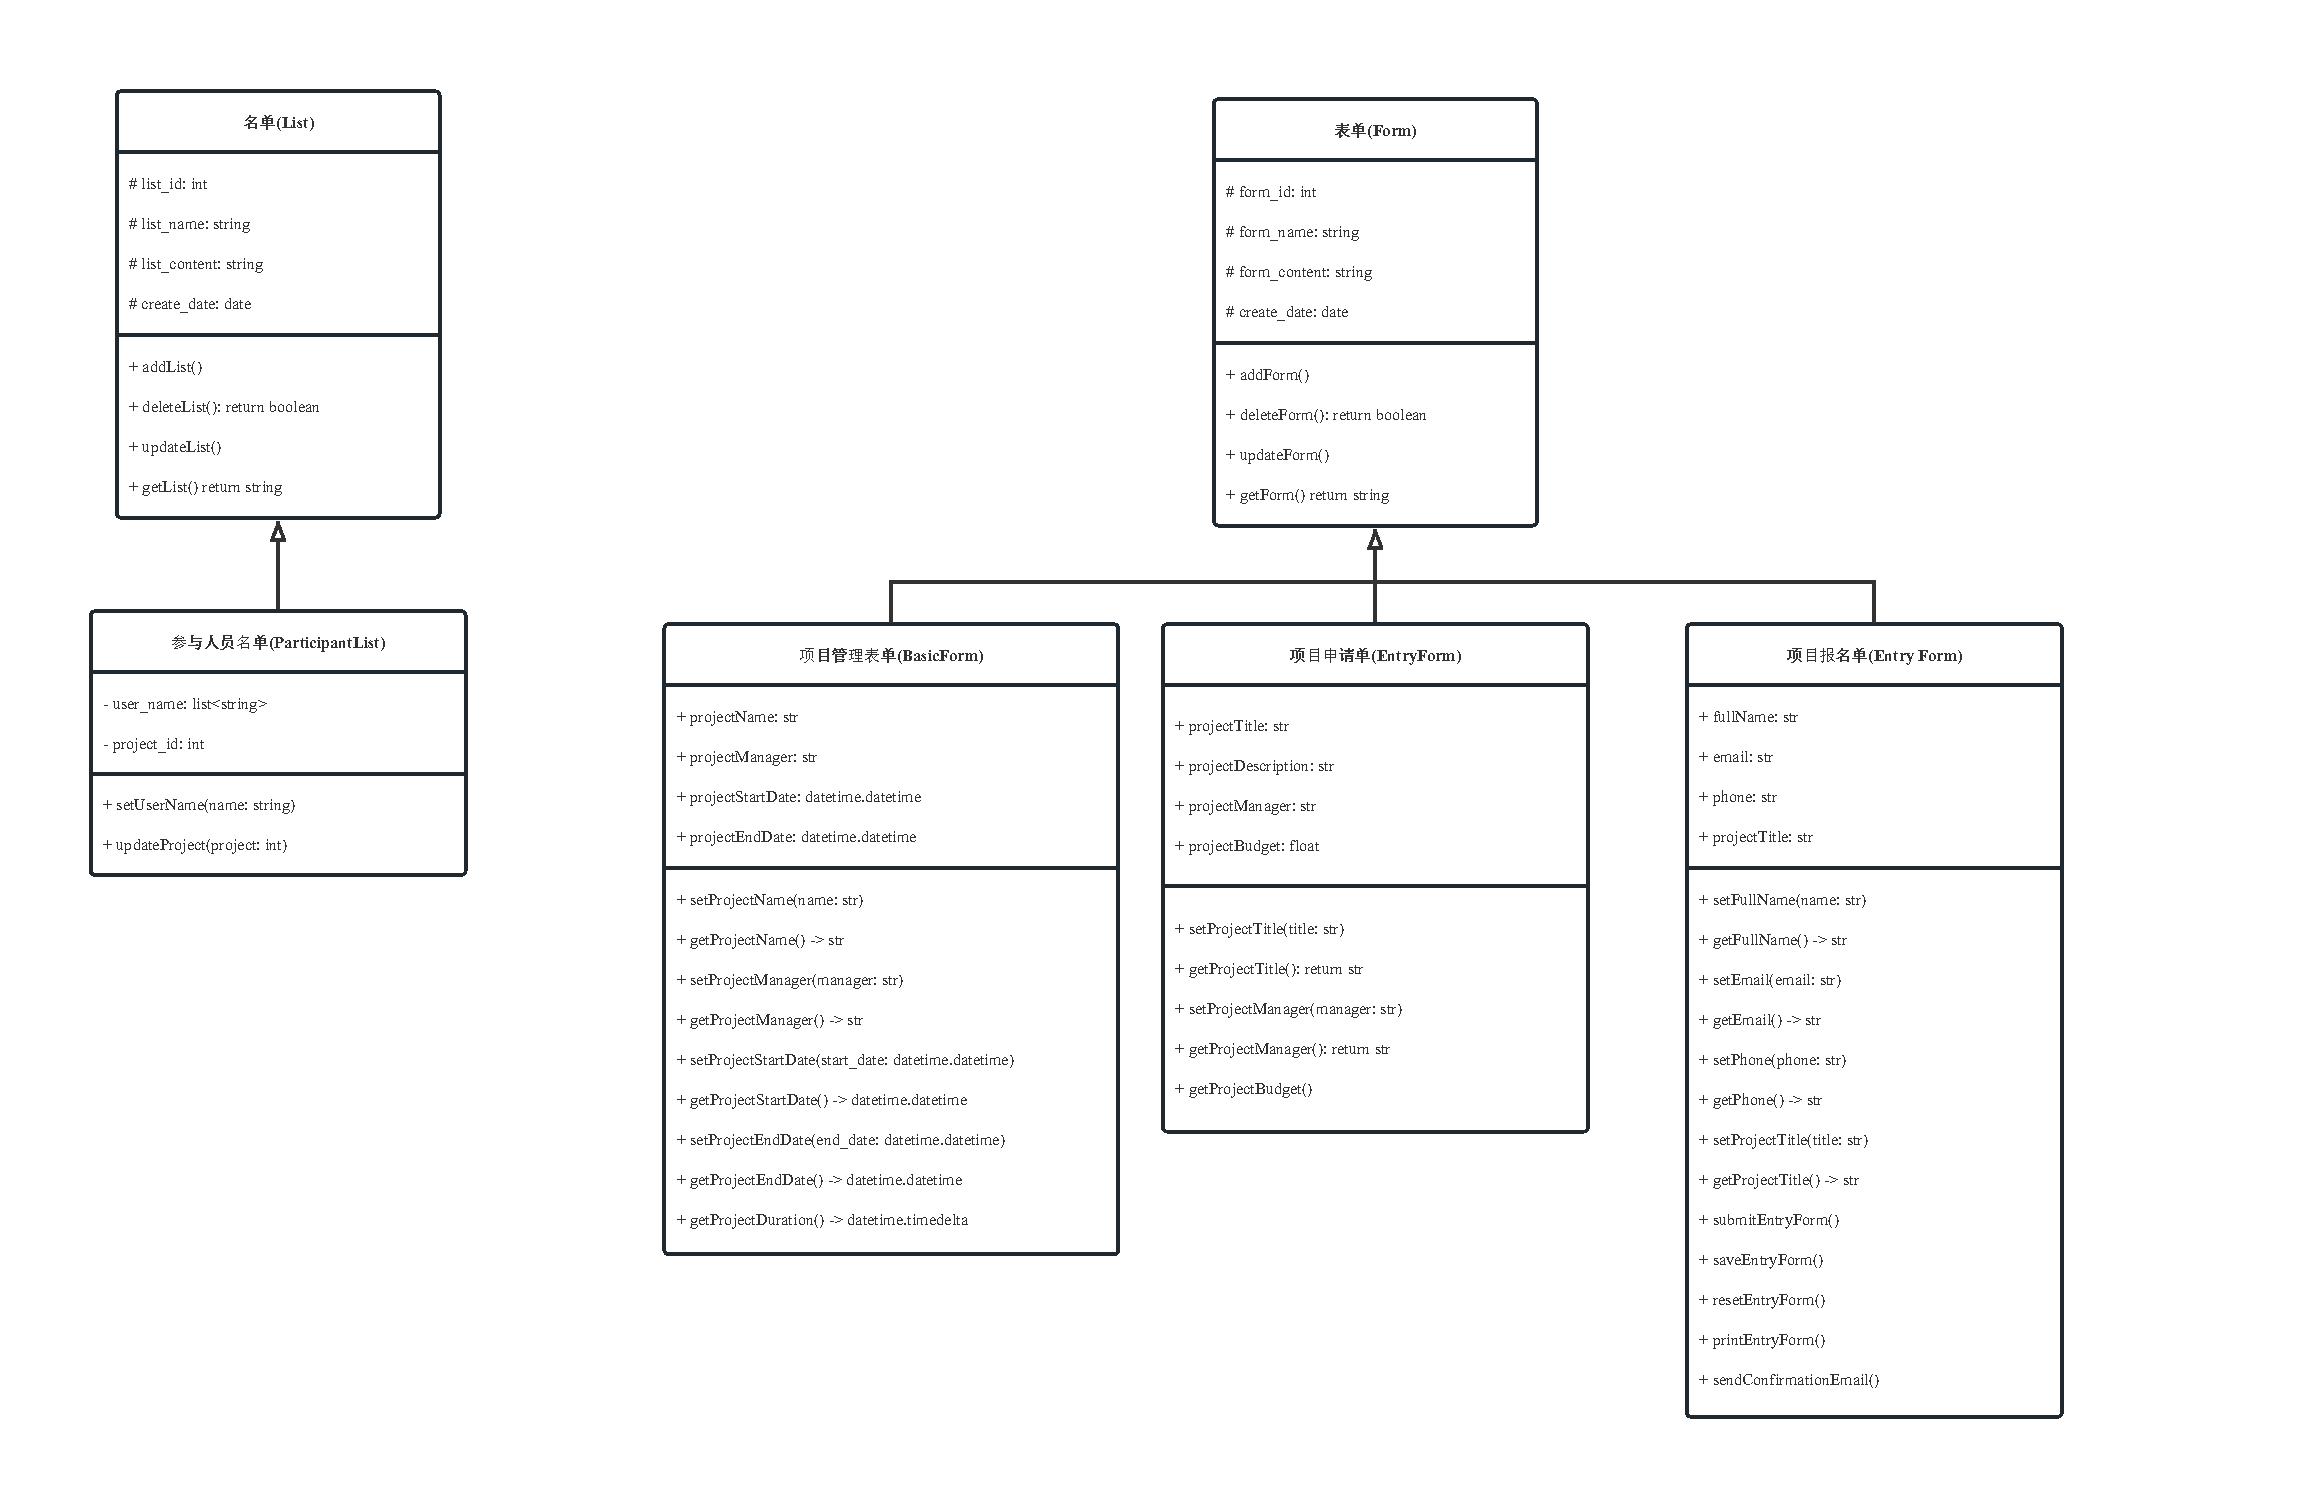
\includegraphics[scale=0.45]{OOA/fig/2-志愿服务/志愿服务类图-2.pdf}} 
    \bicaption{Volunet志愿服务系统类属性与操作2子图}{Class Attributes and Operations Sub-Diagram 2 for Volunteer Service System of Volunet} 
\end{figure}

\paragraph{志愿服务系统类属性与操作描述}~{}

志愿服务系统中类包含用户、志愿者、志愿团队、系统管理员、名单、参与人员名单、表单、项目申请单、项目报名单、项目管理表单,它们的属性与操作描述如下:

% 用户、志愿者、志愿团队、系统管理员、名单、参与人员名单、表单、
\begin{table}[H]  
\caption{“用户”类词条描述}  
\begin{center}  
    \begin{tabular}{l p{11cm}} 
        \hline
        \quad 名称:  &  用户 \\
        \hline
        \quad 编号:  & 2.1 \\
        \hline
        \quad 英文:  &  User \\
        \hline
        \quad 简述:  & 使用志愿服务系统的个人或组织的统称 \\
        \hline
        \quad 属性:  & id、username、password、name、age、contact \\
        \hline
        \quad 操作:  & setPassword()、getId()、getName()、getAge() 、login()、logout() \\
        \hline
        \quad 相关类:  & 志愿者、志愿团队、系统管理员 \\
        \hline
    \end{tabular}
\end{center}
\end{table}

\begin{table}[H]  
\caption{“志愿团队”类词条描述}  
\begin{center}  
    \begin{tabular}{l p{11cm}} 
        \hline
        \quad 名称:  &  志愿团队 \\
        \hline
        \quad 编号:  & 2.2 \\
        \hline
        \quad 英文:  &  Team \\
        \hline
        \quad 简述:  & 使用志愿服务系统发布志愿项目的组织 \\
        \hline
        \quad 属性:  & category、team\_name \\
        \hline 
        \quad 操作:  & getName()、getDescription()、getLeader()、getMembers()、addMember()、removeMember()、getProjects()、addProject()、removeProject()、getMission()、setMission()
\\
        \hline
        \quad 相关类:  & 用户、项目申请单、志愿者 \\
        \hline
    \end{tabular}
\end{center}
\end{table}

\begin{table}[H]  
\caption{“志愿者”类词条描述}  
\begin{center}  
    \begin{tabular}{l p{11cm}} 
        \hline
        \quad 名称:  &  志愿者 \\
        \hline
        \quad 编号:  & 2.3 \\
        \hline
        \quad 英文:  &  Volunteer \\
        \hline
        \quad 简述:  & 使用志愿服务系统对参与志愿项目的人 \\
        \hline
        \quad 属性:  & gender、volunteer\_name
 \\
        \hline
        \quad 操作:  & setGender()、getGender()、queryVolunteer()、queryTeam()、createForm()
 \\
        \hline
        \quad 相关类:  & 用户、志愿团队、项目报名单 \\
        \hline
    \end{tabular}
\end{center}
\end{table}

\begin{table}[H]  
\caption{“系统管理员”类词条描述}  
\begin{center}  
    \begin{tabular}{l p{11cm}} 
        \hline
        \quad 名称:  &  系统管理员 \\
        \hline
        \quad 编号:  & 2.4 \\
        \hline
        \quad 英文:  &  Administrator \\
        \hline
        \quad 简述:  & 管理志愿服务系统,进行信息审核的人 \\
        \hline
        \quad 属性:  & permissions \\
        \hline
        \quad 操作:  & updateUser()、manageVolunteer()、manageTeam()、manageForm()\\
        \hline
        \quad 相关类:  & 用户、审核系统\\
        \hline
    \end{tabular}
\end{center}
\end{table}

\begin{table}[H]  
\caption{“名单”类词条描述}  
\begin{center}  
    \begin{tabular}{l p{11cm}} 
        \hline
        \quad 名称:  &  名单 \\
        \hline
        \quad 编号:  & 2.5 \\
        \hline
        \quad 英文:  &  List \\
        \hline
        \quad 简述:  & 按照一定标准或规则列出的人员或事物清单 \\
        \hline
        \quad 属性:  &list\_id、list\_name、list\_content、create\_date\\
        \hline
        \quad 操作:  & addList()、deleteList()、updateList()、getList() \\
        \hline
        \quad 相关类:  & 参与人员名单 \\
        \hline
    \end{tabular}
\end{center}
\end{table}

\begin{table}[H]  
\caption{“参与人员名单”类词条描述}  
\begin{center}  
    \begin{tabular}{l p{11cm}} 
        \hline
        \quad 名称:  &  参与人员名单 \\
        \hline
        \quad 编号:  & 2.6 \\
        \hline
        \quad 英文:  &  ParticipantList \\
        \hline
        \quad 简述:  & 参与志愿项目的公示名单 \\
        \hline
        \quad 属性:  & user\_name、project\_id
\\
        \hline
        \quad 操作:  & setUserName()、updateProject()

\\
        \hline
        \quad 相关类:  & 名单、志愿团队 \\
        \hline
    \end{tabular}
\end{center}
\end{table}

\begin{table}[H]  
\caption{“表单”类词条描述}  
\begin{center}  
    \begin{tabular}{l p{11cm}} 
        \hline
        \quad 名称:  &  表单 \\
        \hline
        \quad 编号:  & 2.7 \\
        \hline
        \quad 英文:  &  Form \\
        \hline
        \quad 简述:  & 用于收集、记录和处理信息的文档或工具 \\
        \hline
        \quad 属性:  & form\_id、form\_name、form\_content、create\_date: date\\
        \hline
        \quad 操作:  & addForm()、deleteForm()、updateForm()、getForm()\\
        \hline
        \quad 相关类:  & 项目申请单、项目报名单、项目管理名单 \\
        \hline
    \end{tabular}
\end{center}
\end{table}

\begin{table}[H]  
\caption{“项目申请单”类词条描述}  
\begin{center}  
    \begin{tabular}{l p{11cm}} 
        \hline
        \quad 名称:  &  项目申请单 \\
        \hline
        \quad 编号:  & 2.8 \\
        \hline
        \quad 英文:  & EntryForm\\
        \hline
        \quad 简述:  & 用于提交和审批志愿项目计划的表单 \\
        \hline
        \quad 属性:  & projectTitle、projectDescription、projectManager、projectBudget\\
        \hline
        \quad 操作:  & setProjectTitle()、getProjectTitle()、setProjectManager()、getProjectManager()、getProjectBudget()\\
        \hline
        \quad 相关类:  & 表单、系统管理员、志愿团队 \\
        \hline
    \end{tabular}
\end{center}
\end{table}

\begin{table}[H]  
\caption{“项目报名单”类词条描述}  
\begin{center}  
    \begin{tabular}{l p{11cm}} 
        \hline
        \quad 名称:  &  项目报名单 \\
        \hline
        \quad 编号:  & 2.9 \\
        \hline
        \quad 英文:  &  EntryForm \\
        \hline
        \quad 简述:  & 收集志愿项目参与者信息的表单 \\
        \hline
        \quad 属性:  & fullName、email、phone、projectTitle\\
        \hline
        \quad 操作:  & setFullName()、getFullName()、setEmail()、getEmail()、setPhone()、getPhone()、setProjectTitle(title: str)、getProjectTitle()、submitEntryForm()、saveEntryForm()、resetEntryForm()、printEntryForm()、sendConfirmationEmail()
\\
        \hline
        \quad 相关类:  & 表单、志愿者、系统管理员 \\
        \hline
    \end{tabular}
\end{center}
\end{table}

\begin{table}[H]  
\caption{“项目管理表单”类词条描述}  
\begin{center}  
    \begin{tabular}{l p{11cm}} 
        \hline
        \quad 名称:  &  项目管理表单 \\
        \hline
        \quad 编号:  & 2.10 \\
        \hline
        \quad 英文:  &  BasicForm \\
        \hline
        \quad 简述:  & 用于记录和跟踪志愿项目管理信息的表单 \\
        \hline
        \quad 属性:  & projectName、projectManager、projectStartDate、projectEndDate\\
        \hline
        \quad 操作:  & setProjectName()、getProjectName()、setProjectManager()、getProjectManager()、setProjectStartDate()、getProjectStartDate()、setProjectEndDate()、getProjectEndDate()、getProjectDuration()\\
        \hline
        \quad 相关类:  & 志愿者、志愿团队、表单 \\
        \hline
    \end{tabular}
\end{center}
\end{table}


\subsubsection{爱心捐助系统}

\paragraph{爱心捐助系统类属性与操作图}~{}
\begin{figure}[H] 
    \center{\includegraphics[scale=0.3, angle=-90]{OOA/fig/3-爱心管理/爱心管理类图-2.pdf}} 
    \bicaption{Volunet爱心捐助系统类属性与操作1子图}{Class Attributes and Operations Sub-Diagram 1 for Love Donation System of Volunet} 
\end{figure}

\begin{figure}[H] 
    \center{\includegraphics[scale=0.35]{OOA/fig/3-爱心管理/爱心管理类图-3.pdf}} 
    \bicaption{Volunet爱心捐助系统类属性与操作2子图}{Class Attributes and Operations Sub-Diagram 2 for Love Donation System of Volunet} 
\end{figure}

\paragraph{爱心捐助系统类属性与操作描述}~{}

爱心捐助系统中类包含用户、捐款者、志愿团队、购买者、公益商户、系统管理员、订单、证书、爱心证书、名单、鸣谢名单、系统、授课系统、订单系统、捐款系统以及爱心反馈系统,它们的属性与操作描述如下:

% 捐款者、志愿团队、购买者、公益商户、系统管理员、订单、证书、爱心证书、名单、鸣谢名单、系统、授课系统、订单系统、捐款系统以及爱心反馈系统
\begin{table}[H]  
\caption{“用户”类词条描述}  
\begin{center}  
    \begin{tabular}{l p{11cm}} 
        \hline
        \quad 名称:  &  用户 \\
        \hline
        \quad 编号:  & 3.1 \\
        \hline
        \quad 英文:  &  User \\
        \hline
        \quad 简述:  & 使用爱心捐助系统的个人或组织的统称 \\
        \hline
        \quad 属性:  & id、username、password、name、age、contact \\
        \hline
        \quad 操作:  & setPassword()、getId()、getName()、getAge() 、login()、logout() \\
        \hline
        \quad 相关类:  & 捐款者、志愿团队、购买者、公益商户、系统管理员 \\
        \hline
    \end{tabular}
\end{center}
\end{table}

\begin{table}[H]  
\caption{“志愿团队”类词条描述}  
\begin{center}  
    \begin{tabular}{l p{11cm}} 
        \hline
        \quad 名称:  &  志愿团队 \\
        \hline
        \quad 编号:  & 3.2 \\
        \hline
        \quad 英文:  &  Team \\
        \hline
        \quad 简述:  & 使用爱心捐助系统接收项目捐助的组织 \\
        \hline
        \quad 属性:  & category、team\_name \\
        \hline 
        \quad 操作:  & setProject()、getProject()、queryProject()、queryDonor()、queryDonation()、applyCourse()、getProjectAnalysis()、modifyProject()、getLoveFeedback()\\
        \hline
        \quad 相关类:  & 用户、捐款系统 \\
        \hline
    \end{tabular}
\end{center}
\end{table}

\begin{table}[H]  
\caption{“捐款者”类词条描述}  
\begin{center}  
    \begin{tabular}{l p{11cm}} 
        \hline
        \quad 名称:  &  捐款者 \\
        \hline
        \quad 编号:  & 3.3 \\
        \hline
        \quad 英文:  &  Donor \\
        \hline
        \quad 简述:  & 使用爱心捐助系统对项目进行捐款的人 \\
        \hline
        \quad 属性:  & category、donor\_name\\
        \hline
        \quad 操作:  & setGender()、getGender()、queryTeam()、queryProject()、submitDonation()、queryDonation()、queryCertificate()、queryAcknowledgementList()、\\
        \hline
        \quad 相关类:  & 用户、捐款系统、爱心证书 \\
        \hline
    \end{tabular}
\end{center}
\end{table}

\begin{table}[H]  
\caption{“购买者”类词条描述}  
\begin{center}  
    \begin{tabular}{l p{11cm}} 
        \hline
        \quad 名称:  & 购买者 \\
        \hline
        \quad 编号:  & 3.4 \\
        \hline
        \quad 英文:  &  Buyer \\
        \hline
        \quad 简述:  & 使用爱心捐助系统购买公益商品的人 \\
        \hline
        \quad 属性:  & gender、buyer\_name \\
        \hline
        \quad 操作:  & addOrder()、getOrder()、queryOrder()、modifyOrder()、getLoveFeedback() \\
        \hline
        \quad 相关类:  & 用户、公益商户、订单、订单系统、爱心证书 \\
        \hline
    \end{tabular}
\end{center}
\end{table}

\begin{table}[H]  
\caption{“公益商户”类词条描述}  
\begin{center}  
    \begin{tabular}{l p{11cm}} 
        \hline
        \quad 名称:  &  公益商户 \\
        \hline
        \quad 编号:  & 3.5 \\
        \hline
        \quad 英文:  &  CharitableMerchant \\
        \hline
        \quad 简述:  & 在爱心捐助系统售卖公益商品的人或组织 \\
        \hline
        \quad 属性:  & category、charitable\_merchant\_name \\
        \hline
        \quad 操作:  & handleOrder()、getOrder()、queryOrder()、queryBuyer()、getOrderAnalysis()、getLoveFeedback()\\
        \hline
        \quad 相关类:  & 用户、订单 \\
        \hline
    \end{tabular}
\end{center}
\end{table}

\begin{table}[H]  
\caption{“系统管理员”类词条描述}  
\begin{center}  
    \begin{tabular}{l p{11cm}} 
        \hline
        \quad 名称:  &  系统管理员 \\
        \hline
        \quad 编号:  & 3.6 \\
        \hline
        \quad 英文:  &  Administrator \\
        \hline
        \quad 简述:  & 管理爱心捐助系统,进行信息审核的人 \\
        \hline
        \quad 属性:  & permissions \\
        \hline
        \quad 操作:  & updateUser()、updateLoveFeedback()、reviewQualifications()、reviewDonation()、reviewOrder()、manageCharitableMerchant()、manageBuyer()、manageTeam()、manageDonor()
\\
        \hline
        \quad 相关类:  & 用户、爱心反馈系统、收款系统 \\
        \hline
    \end{tabular}
\end{center}
\end{table}

\begin{table}[H]  
\caption{“订单”类词条描述}  
\begin{center}  
    \begin{tabular}{l p{11cm}} 
        \hline
        \quad 名称:  &  订单 \\
        \hline
        \quad 编号:  & 3.7 \\
        \hline
        \quad 英文:  &  Order \\
        \hline
        \quad 简述:  & 购买者对公益商品所提交的购买请求 \\
        \hline
        \quad 属性:  & order\_id、buyer\_id、charitablemerchant\_id、order\_text、order\_date \\
        \hline
        \quad 操作:  & addOrder()、deleteOrder()、updateOrder()、getOrder()、handelOrder()\\
        \hline
        \quad 相关类:  & 购买者、公益商户、订单系统 \\
        \hline
    \end{tabular}
\end{center}
\end{table}

\begin{table}[H]  
\caption{“证书”类词条描述}  
\begin{center}  
    \begin{tabular}{l p{11cm}} 
        \hline
        \quad 名称:  &  证书 \\
        \hline
        \quad 编号:  & 3.8 \\
        \hline
        \quad 英文:  &  Certificate \\
        \hline
        \quad 简述:  & 对个人或组织具有某种能力、资格或成就的认证文件 \\
        \hline
        \quad 属性:  & cert\_id、cert\_name、issue、issue\_date\\
        \hline
        \quad 操作:  & awardCert()、revokeCert() \\
        \hline
        \quad 相关类:  & 爱心证书 \\
        \hline
    \end{tabular}
\end{center}
\end{table}

\begin{table}[H]  
\caption{“爱心证书”类词条描述}  
\begin{center}  
    \begin{tabular}{l p{11cm}} 
        \hline
        \quad 名称:  &  爱心证书 \\
        \hline
        \quad 编号:  & 3.9 \\
        \hline
        \quad 英文:  &  LoveCertificate \\
        \hline
        \quad 简述:  & 对爱心人士进行感谢和认证的文件 \\
        \hline
        \quad 属性:  & user\_name、content\\
        \hline
        \quad 操作:  & setUserName()、setContent()\\
        \hline
        \quad 相关类:  & 证书、捐款者、购买者、订单系统、捐款系统 \\
        \hline
    \end{tabular}
\end{center}
\end{table}

\begin{table}[H]  
\caption{“名单”类词条描述}  
\begin{center}  
    \begin{tabular}{l p{11cm}} 
        \hline
        \quad 名称:  &  名单 \\
        \hline
        \quad 编号:  & 3.10 \\
        \hline
        \quad 英文:  &  List \\
        \hline
        \quad 简述:  & 按照一定标准或规则列出的人员或事物清单 \\
        \hline
        \quad 属性:  &list\_id、list\_name、list\_content、create\_date\\
        \hline
        \quad 操作:  & addList()、deleteList()、updateList()、getList() \\
        \hline
        \quad 相关类:  & 鸣谢名单 \\
        \hline
    \end{tabular}
\end{center}
\end{table}

\begin{table}[H]  
\caption{“鸣谢名单”类词条描述}  
\begin{center}  
    \begin{tabular}{l p{11cm}} 
        \hline
        \quad 名称:  &  鸣谢名单 \\
        \hline
        \quad 编号:  & 3.11 \\
        \hline
        \quad 英文:  &  AcknowledgementList \\
        \hline
        \quad 简述:  & 感谢爱心人士的公示名单 \\
        \hline
        \quad 属性:  & user\_name、donation\_money\\
        \hline
        \quad 操作:  & setUserName()、updateDonationMoney()
\\
        \hline
        \quad 相关类:  & 名单、爱心反馈系统 \\
        \hline
    \end{tabular}
\end{center}
\end{table}

\begin{table}[H]  
\caption{“系统”类词条描述}  
\begin{center}  
    \begin{tabular}{l p{11cm}} 
        \hline
        \quad 名称:  &  系统 \\
        \hline
        \quad 编号:  & 3.12 \\
        \hline
        \quad 英文:  &  System \\
        \hline
        \quad 简述:  & 爱心捐助系统的简称 \\
        \hline
        \quad 属性:  & id、name、description、version\\
        \hline
        \quad 操作:  & start()、stop()、update()\\
        \hline
        \quad 相关类:  & 爱心反馈系统、收款系统 \\
        \hline
    \end{tabular}
\end{center}
\end{table}

\begin{table}[H]  
\caption{“爱心反馈系统”类词条描述}  
\begin{center}  
    \begin{tabular}{l p{11cm}} 
        \hline
        \quad 名称:  &  爱心反馈系统 \\
        \hline
        \quad 编号:  & 3.13 \\
        \hline
        \quad 英文:  &  LoveFeedbackSystem \\
        \hline
        \quad 简述:  & 负责对爱心人士进行反馈和感谢的系统 \\
        \hline
        \quad 属性:  & lovefeedbacks\\
        \hline
        \quad 操作:  & addLoveFeedback()、removeLoveFeedback()、getLoveFeedbacks()\\
        \hline
        \quad 相关类:  & 系统、系统管理员、爱心证书、鸣谢名单 \\
        \hline
    \end{tabular}
\end{center}
\end{table}

\begin{table}[H]  
\caption{“收款系统”类词条描述}  
\begin{center}  
    \begin{tabular}{l p{11cm}} 
        \hline
        \quad 名称:  &  收款系统 \\
        \hline
        \quad 编号:  & 3.14 \\
        \hline
        \quad 英文:  &  PaymentSystem \\
        \hline
        \quad 简述:  & 负责捐助款项管理的系统 \\
        \hline
        \quad 属性:  & payment\\
        \hline
        \quad 操作:  & addPayment()、removePayment()、getPayment()、showProgress()、paymentChat()
\\
        \hline
        \quad 相关类:  & 系统、系统管理员、订单系统、捐款系统 \\
        \hline
    \end{tabular}
\end{center}
\end{table}

\begin{table}[H]  
\caption{“订单系统”类词条描述}  
\begin{center}  
    \begin{tabular}{l p{11cm}} 
        \hline
        \quad 名称:  &  订单系统 \\
        \hline
        \quad 编号:  & 3.15 \\
        \hline
        \quad 英文:  &  OrderSystem \\
        \hline
        \quad 简述:  & 负责订单管理的系统 \\
        \hline
        \quad 属性:  & orders、create\_date\\
        \hline
        \quad 操作:  & addOrder()、removeOrder()、getOrders()、getOrderID()、getCreateDate()、orderAnalysis()\\
        \hline
        \quad 相关类:  & 收款系统、订单、购买者、爱心证书、公益商户 \\
        \hline
    \end{tabular}
\end{center}
\end{table}

\begin{table}[H]  
\caption{“捐款系统”类词条描述}  
\begin{center}  
    \begin{tabular}{l p{11cm}} 
        \hline
        \quad 名称:  &  捐款系统 \\
        \hline
        \quad 编号:  & 3.16 \\
        \hline
        \quad 英文:  &  DonationSystem \\
        \hline
        \quad 简述:  & 负责捐款管理的系统 \\
        \hline
        \quad 属性:  & donations、donation\_date\\
        \hline
        \quad 操作:  & addDonation()、removeDonation()、getDonations()、donationAnalysis()、getDonationDate()\\
        \hline
        \quad 相关类:  & 收款系统、捐款者、爱心证书、志愿团队 \\
        \hline
    \end{tabular}
\end{center}
\end{table}



\subsubsection{公益课程系统}

\paragraph{公益课程系统类属性与操作图}~{}
\begin{figure}[H] 
    \center{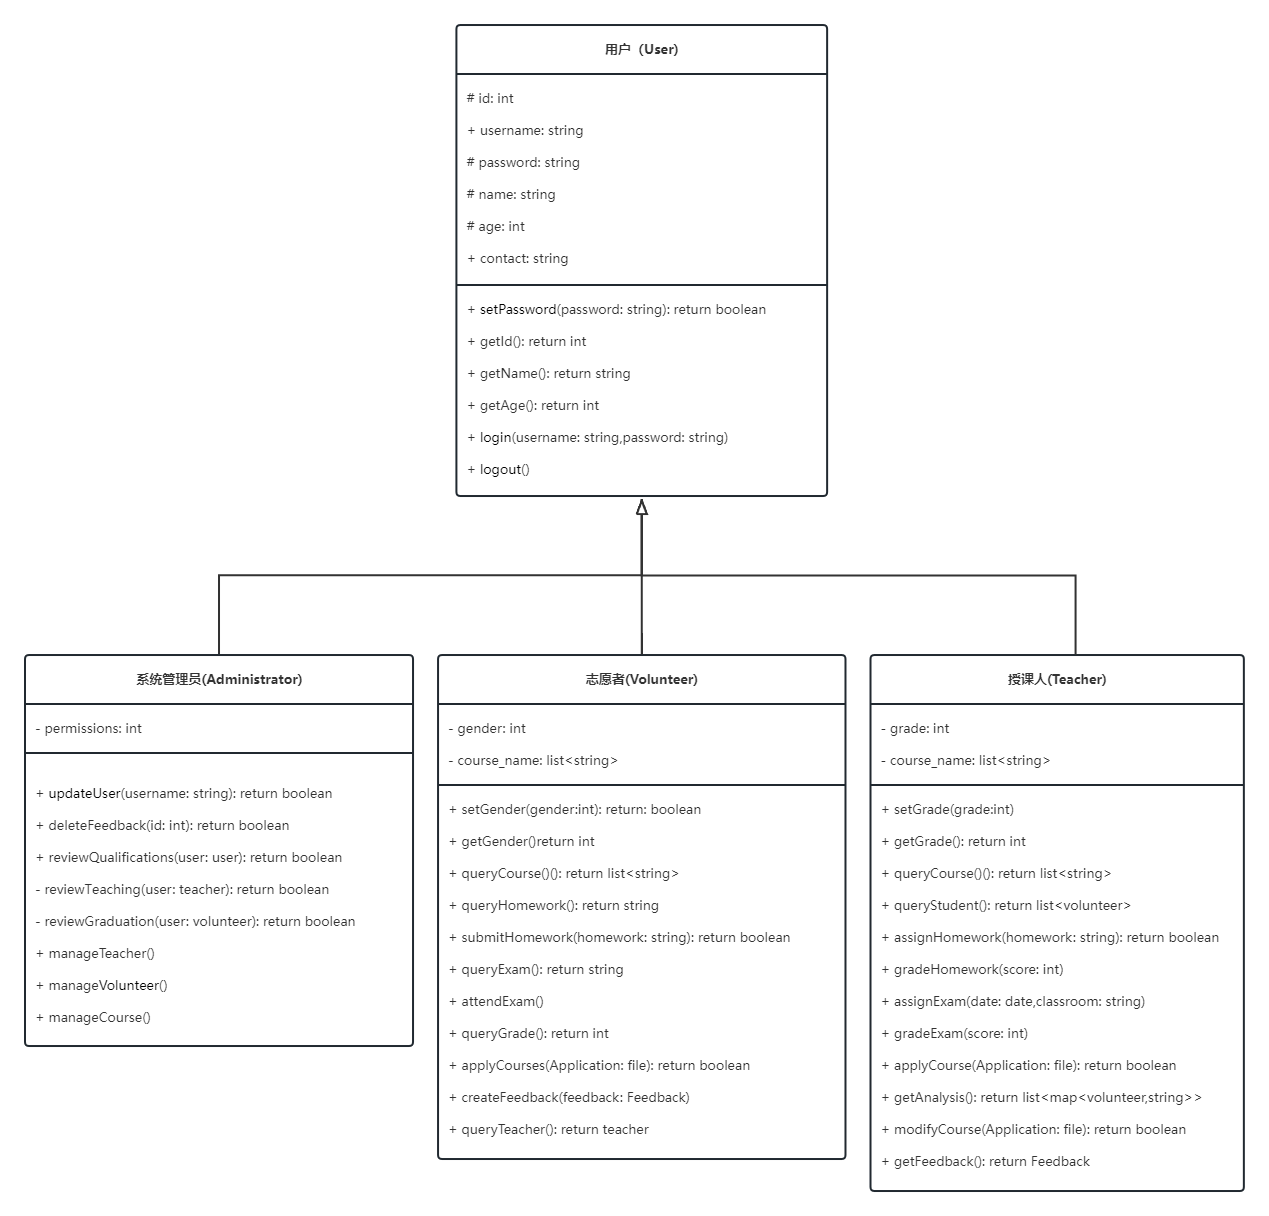
\includegraphics[scale=0.33]{OOA/fig/4-课程管理/课程管理类图 (1).png}} 
    \bicaption{Volunet公益课程系统类属性与操作1子图}{Class Attributes and Operations Sub-Diagram 1 for Course System of Volunet} 
\end{figure}

\begin{figure}[H] 
    \center{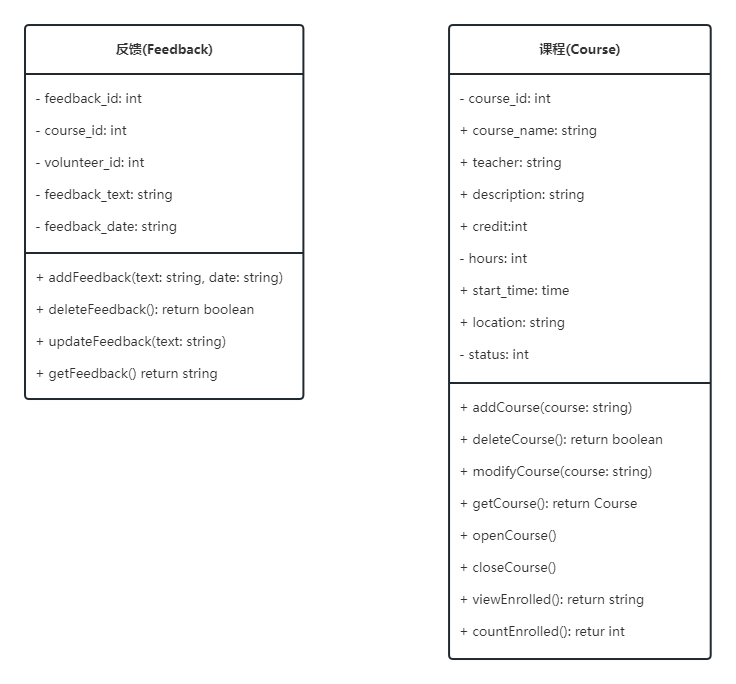
\includegraphics[scale=0.33]{OOA/fig/4-课程管理/课程管理类图 (2).png}} 
    \center{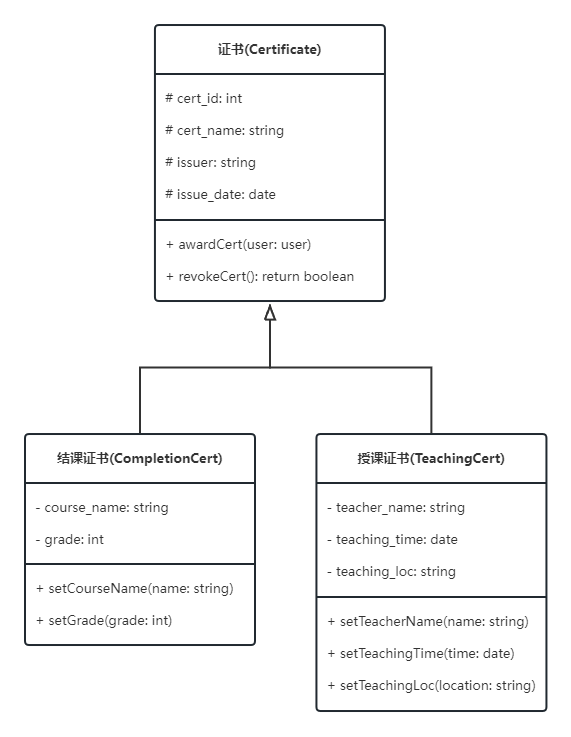
\includegraphics[scale=0.33]{OOA/fig/4-课程管理/课程管理类图 (3).png}} 
    \bicaption{Volunet公益课程系统类属性与操作2子图}{Class Attributes and Operations Sub-Diagram 2 for Course System of Volunet} 
\end{figure}

\begin{figure}[H] 
    \center{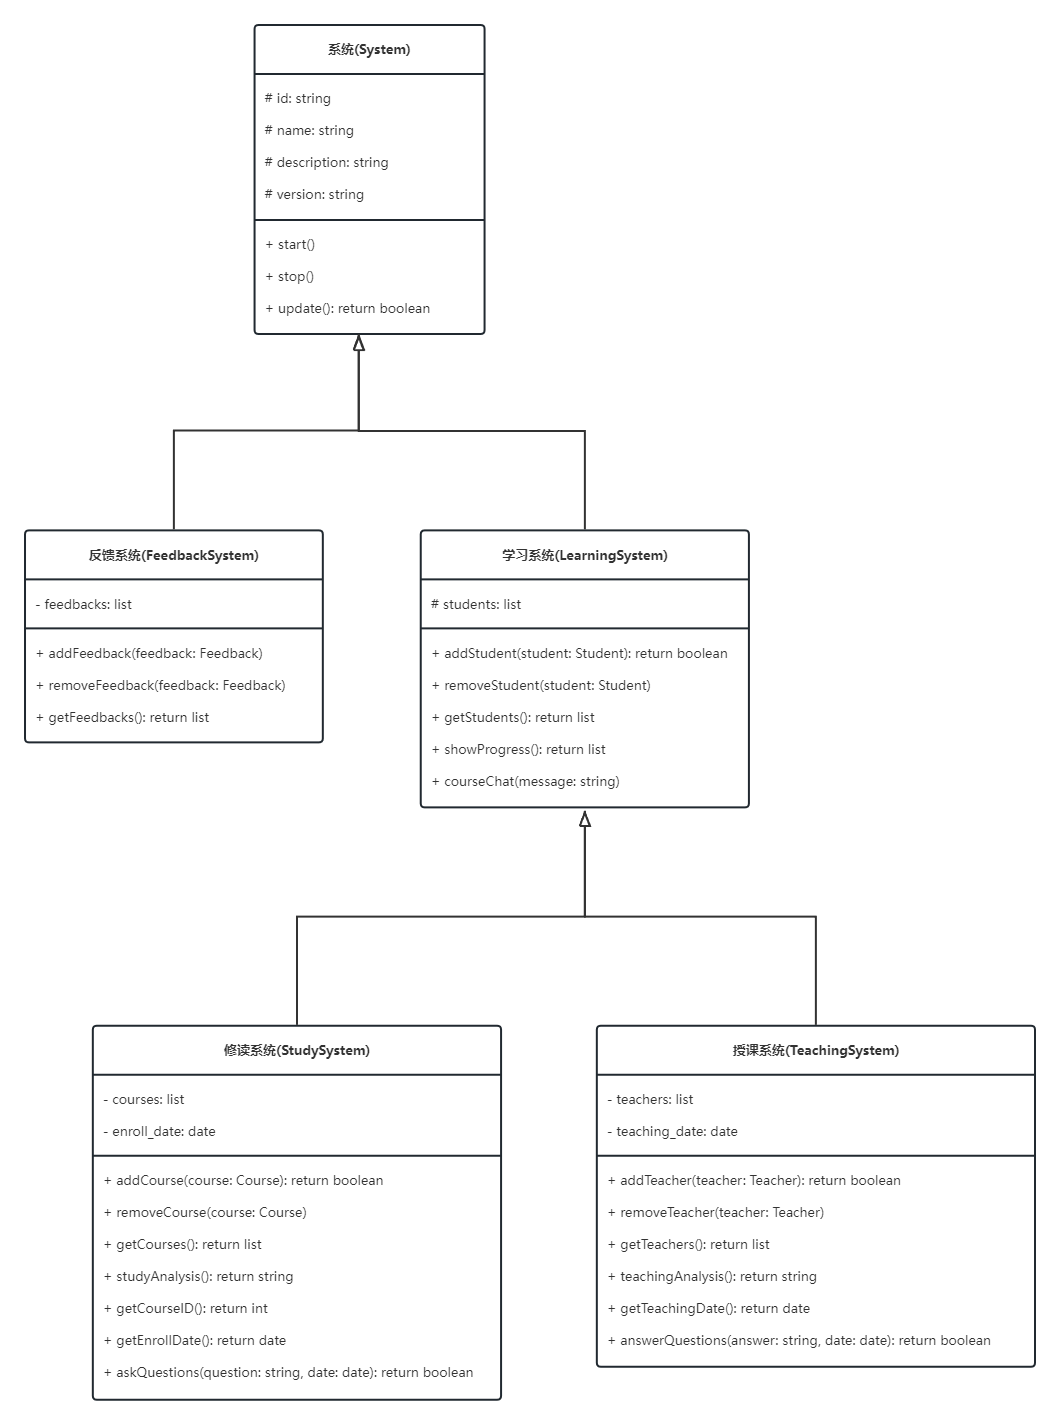
\includegraphics[scale=0.33]{OOA/fig/4-课程管理/课程管理类图 (4).png}} 
    \bicaption{Volunet公益课程系统类属性与操作3子图}{Class Attributes and Operations Sub-Diagram 3 for Course System of Volunet} 
\end{figure}

\paragraph{公益课程系统类属性与操作描述}~{}

公益课程系统中类包含用户、系统管理员、志愿者、授课人、反馈、课程、证书、结课证书、授课证书、系统、反馈系统、学习系统、修读系统、授课系统,它们的属性与操作描述如下:

% 用户、系统管理员、志愿者、授课人、反馈、课程、证书、结课证书、授课证书、系统、反馈系统、学习系统、修读系统、授课系统
\begin{table}[H]  
\caption{“用户”类词条描述}  
\begin{center}  
    \begin{tabular}{l p{11cm}} 
        \hline
        \quad 名称:  &  用户 \\
        \hline
        \quad 编号:  & 4.1 \\
        \hline
        \quad 英文:  &  User \\
        \hline
        \quad 简述:  & 使用课程管理系统的个人的统称 \\
        \hline
        \quad 属性:  & id、username、password、name、age、contact \\
        \hline
        \quad 操作:  & setPassword()、getId()、getName()、getAge() 、login()、logout() \\
        \hline
        \quad 相关类:  & 志愿者、授课人、系统管理员 \\
        \hline
    \end{tabular}
\end{center}
\end{table}


\begin{table}[H]  
\caption{“系统管理员”类词条描述}  
\begin{center}  
    \begin{tabular}{l p{11cm}} 
        \hline
        \quad 名称:  &  系统管理员 \\
        \hline
        \quad 编号:  & 4.2 \\
        \hline
        \quad 英文:  &  Administrator \\
        \hline
        \quad 简述:  & 管理课程信息审核,进行反馈信息审核的人 \\
        \hline
        \quad 属性:  & permissions \\
        \hline
        \quad 操作:  & updateUser()、updateLoveFeedback()、reviewQualifications()、reviewDonation()、reviewOrder()、manageCharitableMerchant()、manageBuyer()、manageTeam()、manageDonor()
\\
        \hline
        \quad 相关类:  & 用户、反馈系统、学习系统 \\
        \hline
    \end{tabular}
\end{center}
\end{table}

\begin{table}[H]  
\caption{“志愿者”类词条描述}  
\begin{center}  
    \begin{tabular}{l p{11cm}} 
        \hline
        \quad 名称:  &  志愿者 \\
        \hline
        \quad 编号:  & 4.3 \\
        \hline
        \quad 英文:  &  Volunteer \\
        \hline
        \quad 简述:  & 使用课程管理系统修读课程,进行课程反馈的人 \\
        \hline
        \quad 属性:  & gender、course\_name \\
        \hline 
        \quad 操作:  & setGender()、getGender()、queryCourse()、queryHomework()、submitHomework()、queryExam()、attendExam()、queryGrade()、applyCourses()、createFeedback()、queryTeacher()\\
        \hline
        \quad 相关类:  & 用户、授课人、修读系统 \\
        \hline
    \end{tabular}
\end{center}
\end{table}

\begin{table}[H]  
\caption{“授课人”类词条描述}  
\begin{center}  
    \begin{tabular}{l p{11cm}} 
        \hline
        \quad 名称:  &  授课人 \\
        \hline
        \quad 编号:  & 4.4 \\
        \hline
        \quad 英文:  &  Teacher \\
        \hline
        \quad 简述:  & 使用课程管理系统对教授课程,回应反馈的人 \\
        \hline
        \quad 属性:  & grade、course\_name \\
        \hline
        \quad 操作:  & setGrade()、getGender()、queryCourse()、queryStudent()、assignHomework()、gradeHomework()、assignExam()、gradeExam()、applyCourse()、getAnalysis()、modifyCourse()、getFeedback() \\
        \hline
        \quad 相关类:  & 用户、志愿者、授课系统 \\
        \hline
    \end{tabular}
\end{center}
\end{table}

\begin{table}[H]  
\caption{“反馈”类词条描述}  
\begin{center}  
    \begin{tabular}{l p{11cm}} 
        \hline
        \quad 名称:  &  反馈 \\
        \hline
        \quad 编号:  & 4.5 \\
        \hline
        \quad 英文:  &  Feedback \\
        \hline
        \quad 简述:  & 志愿者对课程所提交的课程评价 \\
        \hline
        \quad 属性:  & feedback\_id、course\_id、volunteer\_id、feedback\_text、feedback\_date \\
        \hline
        \quad 操作:  & addFeedback()、deleteFeedback()、updateFeedback()、getFeedback()\\
        \hline
        \quad 相关类:  & 反馈系统、修读系统、授课系统 \\
        \hline
    \end{tabular}
\end{center}
\end{table}


\begin{table}[H]  
\caption{“课程”类词条描述}  
\begin{center}  
    \begin{tabular}{l p{11cm}} 
        \hline
        \quad 名称:  &  课程 \\
        \hline
        \quad 编号:  & 4.6 \\
        \hline
        \quad 英文:  &  Course \\
        \hline
        \quad 简述:  & 授课人发布的提高志愿者相关公益技能的项目 \\
        \hline
        \quad 属性:  & course\_id、course\_name、teacher、description、credit、hours、start\_time、location、status \\
        \hline
        \quad 操作:  & addCourse()、deleteCourse()、modifyCourse()、getCourse()、openCourse()、closeCourse()、viewEnrolled()、countEnrolled()\\
        \hline
        \quad 相关类:  & 修读系统、授课系统 \\
        \hline
    \end{tabular}
\end{center}
\end{table}

\begin{table}[H]  
\caption{“证书”类词条描述}  
\begin{center}  
    \begin{tabular}{l p{11cm}} 
        \hline
        \quad 名称:  &  证书 \\
        \hline
        \quad 编号:  & 4.7 \\
        \hline
        \quad 英文:  &  Certificate \\
        \hline
        \quad 简述:  & 对个人或组织具有某种能力、资格或成就的认证文件 \\
        \hline
        \quad 属性:  & cert\_id、cert\_name、issue、issue\_date\\
        \hline
        \quad 操作:  & awardCert()、revokeCert() \\
        \hline
        \quad 相关类:  & 授课证书、结课证书 \\
        \hline
    \end{tabular}
\end{center}
\end{table}

\begin{table}[H]  
\caption{“爱心证书”类词条描述}  
\begin{center}  
    \begin{tabular}{l p{11cm}} 
        \hline
        \quad 名称:  &  爱心证书 \\
        \hline
        \quad 编号:  & 4.8 \\
        \hline
        \quad 英文:  &  CompletionCert \\
        \hline
        \quad 简述:  & 对志愿者学习完课程进行认证的文件 \\
        \hline
        \quad 属性:  & user\_name、grade\\
        \hline
        \quad 操作:  & setCourseName()、setGrade()\\
        \hline
        \quad 相关类:  & 修读系统 \\
        \hline
    \end{tabular}
\end{center}
\end{table}

\begin{table}[H]  
\caption{“授课证书”类词条描述}  
\begin{center}  
    \begin{tabular}{l p{11cm}} 
        \hline
        \quad 名称:  &  授课证书 \\
        \hline
        \quad 编号:  & 4.9 \\
        \hline
        \quad 英文:  &  TeachingCert \\
        \hline
        \quad 简述:  & 对授课人可以教授课程进行认证的文件 \\
        \hline
        \quad 属性:  & teacher\_name、teaching\_time、teaching\_loc\\
        \hline
        \quad 操作:  & setTeacherName()、setTeachingTime()、setTeachingLoc() \\
        \hline
        \quad 相关类:  & 授课系统 \\
        \hline
    \end{tabular}
\end{center}
\end{table}

\begin{table}[H]  
\caption{“系统”类词条描述}  
\begin{center}  
    \begin{tabular}{l p{11cm}} 
        \hline
        \quad 名称:  &  系统 \\
        \hline
        \quad 编号:  & 4.10 \\
        \hline
        \quad 英文:  &  System \\
        \hline
        \quad 简述:  & 课程管理系统的简称 \\
        \hline
        \quad 属性:  & id、name、description、version\\
        \hline
        \quad 操作:  & start()、stop()、update()\\
        \hline
        \quad 相关类:  & 学习系统、反馈系统 \\
        \hline
    \end{tabular}
\end{center}
\end{table}

\begin{table}[H]  
\caption{“反馈系统”类词条描述}  
\begin{center}  
    \begin{tabular}{l p{11cm}} 
        \hline
        \quad 名称:  &  反馈系统 \\
        \hline
        \quad 编号:  & 4.11 \\
        \hline
        \quad 英文:  &  FeedbackSystem \\
        \hline
        \quad 简述:  & 负责对课程进行反馈的系统 \\
        \hline
        \quad 属性:  & feedbacks\\
        \hline
        \quad 操作:  & addFeedback()、removeFeedback()、getFeedbacks()\\
        \hline
        \quad 相关类:  & 系统、系统管理员、反馈 \\
        \hline
    \end{tabular}
\end{center}
\end{table}

\begin{table}[H]  
\caption{“学习系统”类词条描述}  
\begin{center}  
    \begin{tabular}{l p{11cm}} 
        \hline
        \quad 名称:  &  学习系统 \\
        \hline
        \quad 编号:  & 4.12 \\
        \hline
        \quad 英文:  &  LearningSystem \\
        \hline
        \quad 简述:  & 负责教授、学习课程的系统 \\
        \hline
        \quad 属性:  & students\\
        \hline
        \quad 操作:  & addStudent()、removeStudent()、getStudents()、showProgress()、courseChat()
\\
        \hline
        \quad 相关类:  & 系统、系统管理员、修读系统、授课系统 \\
        \hline
    \end{tabular}
\end{center}
\end{table}

\begin{table}[H]  
\caption{“修读系统”类词条描述}  
\begin{center}  
    \begin{tabular}{l p{11cm}} 
        \hline
        \quad 名称:  &  修读系统 \\
        \hline
        \quad 编号:  & 4.13 \\
        \hline
        \quad 英文:  &  StudySystem \\
        \hline
        \quad 简述:  & 负责课程学习、管理学生修读进度的系统 \\
        \hline
        \quad 属性:  & courses、enroll\_date\\
        \hline
        \quad 操作:  & addCourse()、removeCourse()、getCourses()、studyAnalysis()、getCourseID()、getEnrollDate()、askQuestions()\\
        \hline
        \quad 相关类:  & 学习系统、反馈、课程、结课证书、志愿者 \\
        \hline
    \end{tabular}
\end{center}
\end{table}

\begin{table}[H]  
\caption{“授课系统”类词条描述}  
\begin{center}  
    \begin{tabular}{l p{11cm}} 
        \hline
        \quad 名称:  &  授课系统 \\
        \hline
        \quad 编号:  & 4.14 \\
        \hline
        \quad 英文:  &  TeachingSystem \\
        \hline
        \quad 简述:  & 负责教授的课程的管理的系统 \\
        \hline
        \quad 属性:  & teachers、teaching\_date\\
        \hline
        \quad 操作:  & addTeacher()、removeTeacher()、getTeachers()、teachingAnalysis()、getTeachingDate()、answerQuestions()\\
        \hline
        \quad 相关类:  & 学习系统、反馈、课程、授课证书、授课人 \\
        \hline
    \end{tabular}
\end{center}
\end{table}


\subsubsection{交流论坛系统}

\paragraph{交流论坛系统类属性与操作图}~{}
\begin{figure}[H] 
    \center{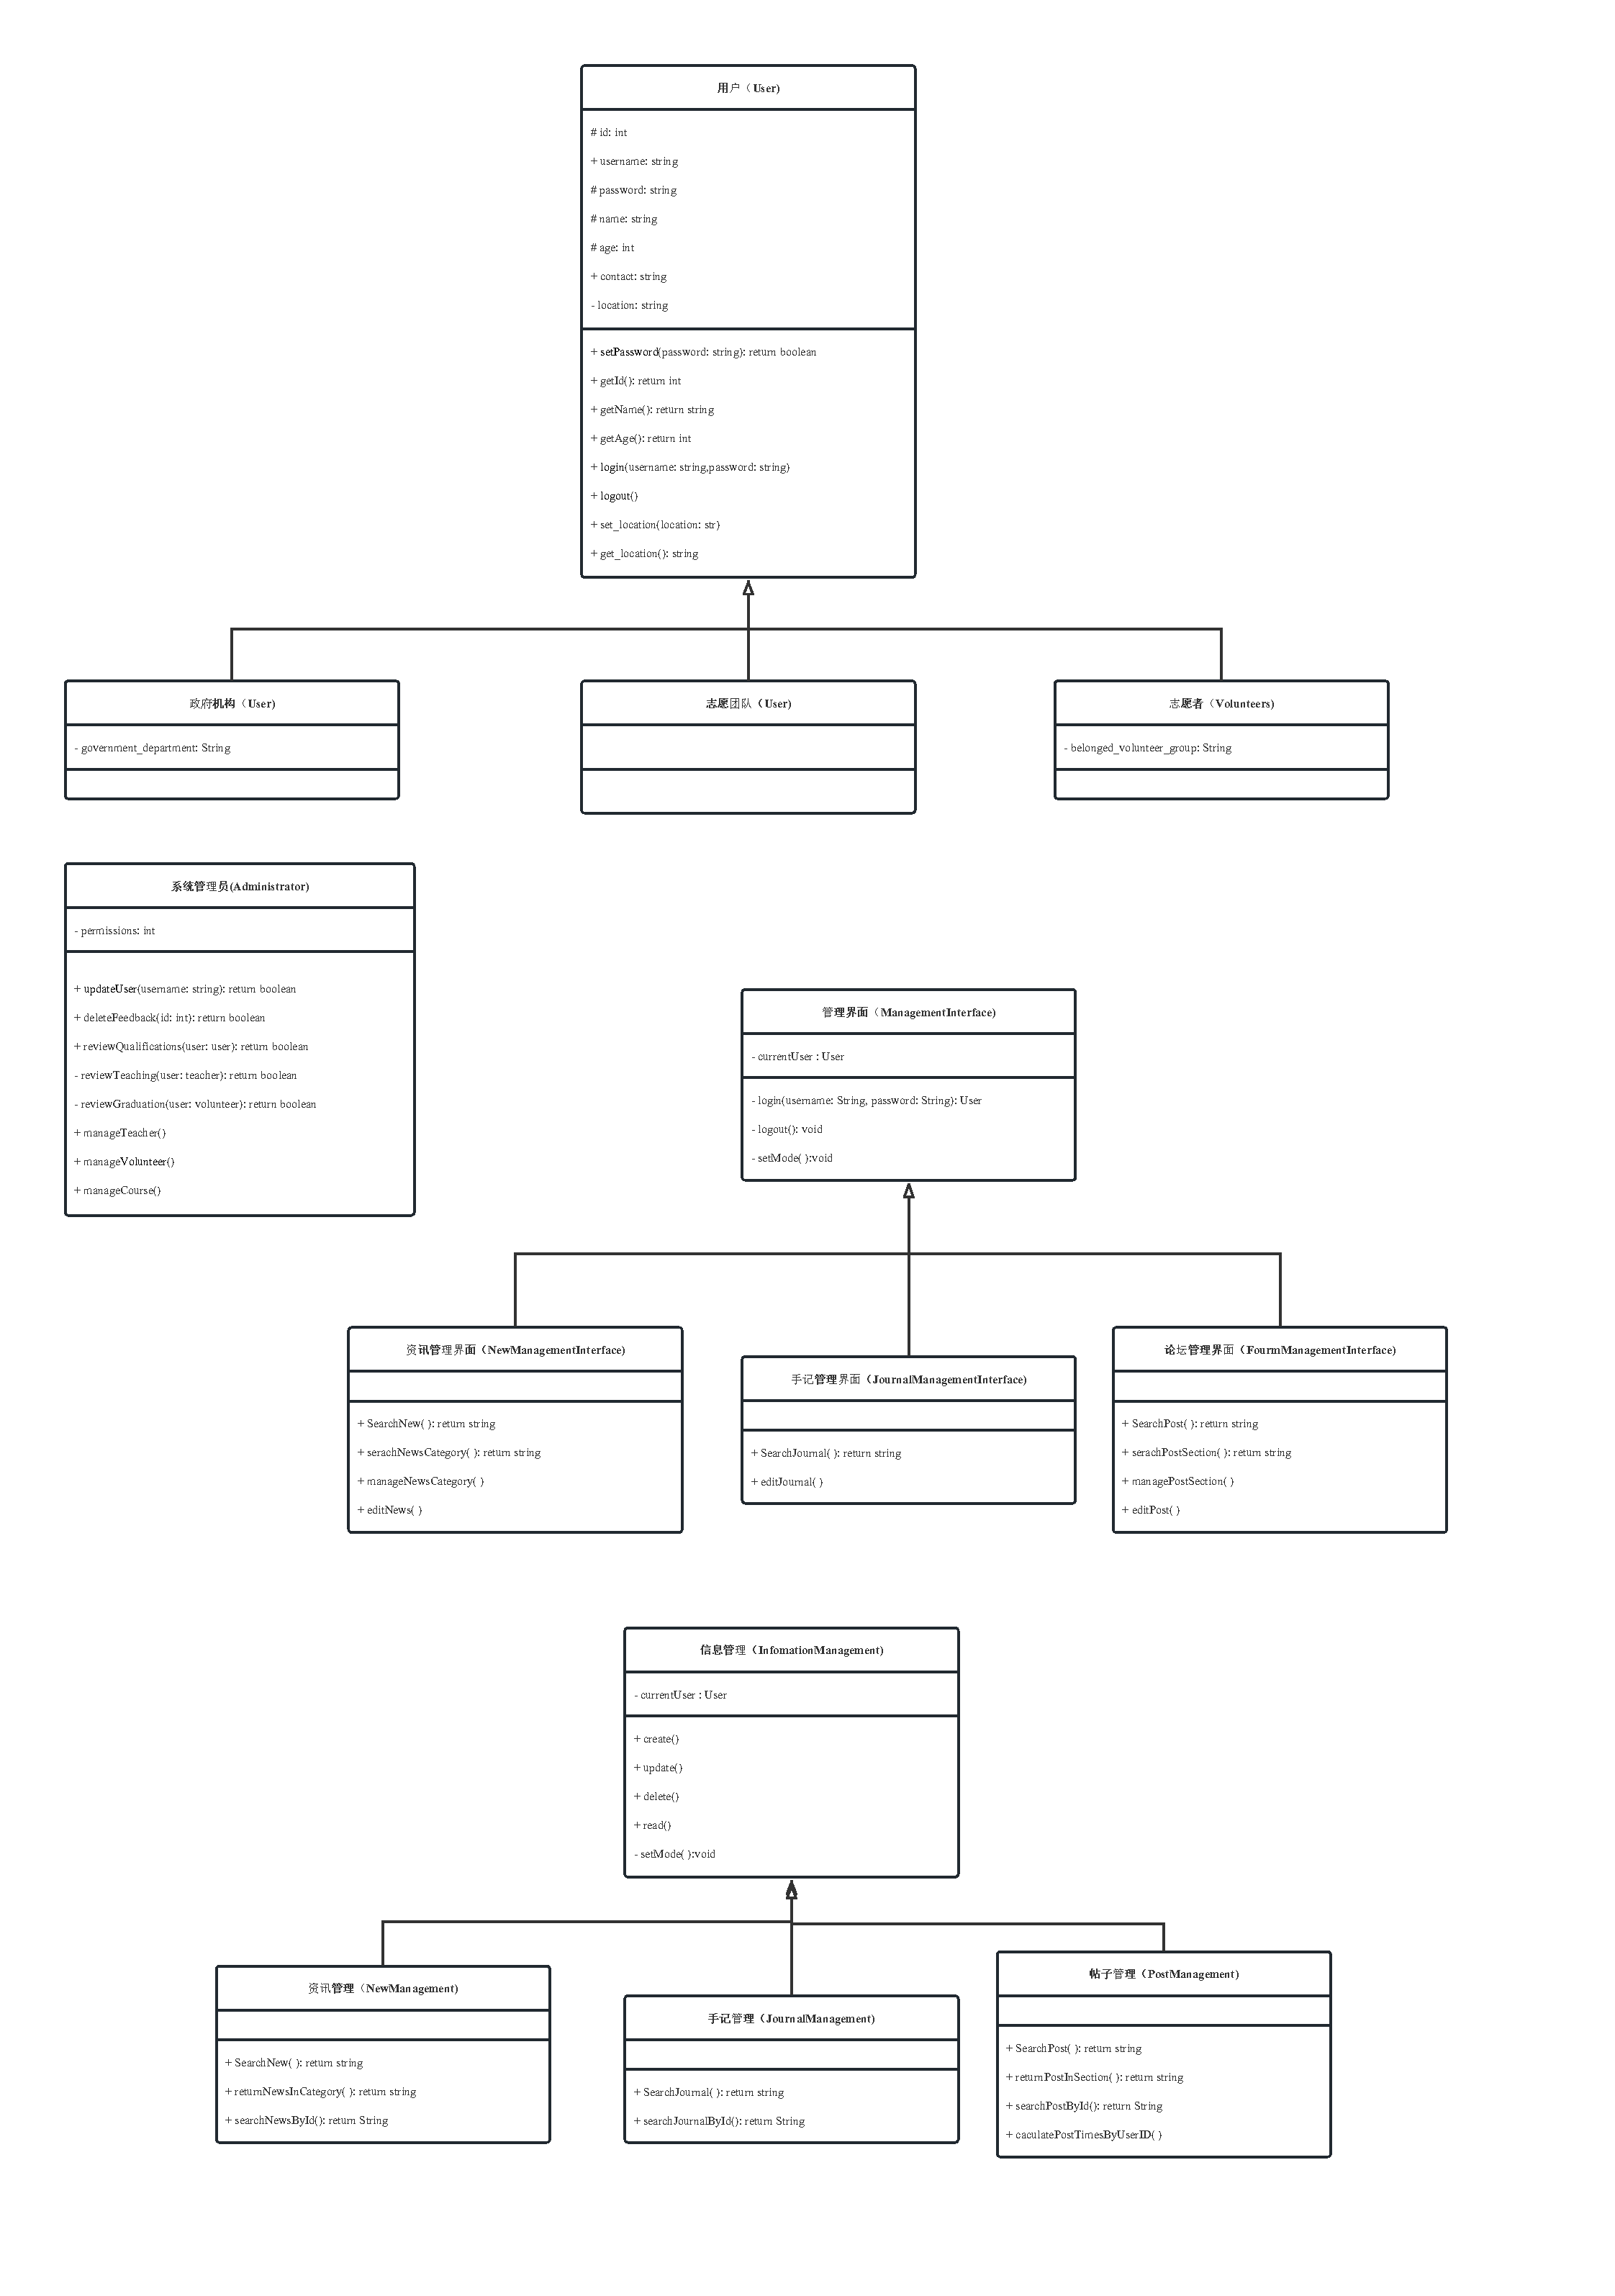
\includegraphics[scale=0.33]{OOA/fig/5-论坛管理/论坛管理类图属性与操作-1.pdf}} 
    \bicaption{Volunet交流论坛系统类属性与操作1子图}{Class Attributes and Operations Sub-Diagram 1 for Communication System of Volunet} 
\end{figure}

% \begin{figure}[H] 
%     \center{\includegraphics[scale=0.33]{OOA/fig/5-论坛管理/论坛管理类图属性与操作-2.pdf}} 
%     \bicaption{Volunet交流论坛系统类属性与操作2子图}{Class Attributes and Operations Sub-Diagram 2 for Communi
%     System of Volunet} 
% \end{figure}

\paragraph{交流论坛系统类属性与操作描述}~{}

交流论坛系统中类包含用户、志愿者、志愿团队、政府结构、管理界面、资讯管理界面、手记管理界面、论坛管理界面、资讯类别管理、资讯管理、资讯评论管理、手记管理、手机评论管理、帖子管理、回帖管理、板块管理、资讯类别、资讯信息、资讯评论、手记信息、手记评论、帖子讯息、板块信息、审计报表生成,它们的属性与操作描述如下:

\begin{table}[H]  
\caption{“系统管理员”类词条描述}  
\begin{center}  
    \begin{tabular}{l p{11cm}} 
        \hline
        \quad 名称:  &  系统管理员 \\
        \hline
        \quad 编号:  & 5.1 \\
        \hline
        \quad 英文:  &  Administrator \\
        \hline
        \quad 简述:  & 交流论坛系统中的管理员 \\
        \hline
        \quad 属性:  & id、username、password、permissions \\
        \hline
        \quad 操作:  & setPassword()、getId()、manageAuditing()、InformationReviewing() \\
        \hline
        \quad 相关类:  & 志愿者、志愿团队、政府机构、管理界面 \\
        \hline
    \end{tabular}
\end{center}
\end{table}

\begin{table}[H]  
\caption{“用户”类词条描述}  
\begin{center}  
    \begin{tabular}{l p{11cm}} 
        \hline
        \quad 名称:  &  用户 \\
        \hline
        \quad 编号:  & 5.2 \\
        \hline
        \quad 英文:  &  User \\
        \hline
        \quad 简述:  & 交流论坛系统中参与的个体的统称 \\
        \hline
        \quad 属性:  & id、username、password、name、age、contact \\
        \hline
        \quad 操作:  & setPassword()、getId()、getName()、getAge() 、login()、logout() \\
        \hline
        \quad 相关类:  & 志愿者、志愿团队、政府机构、管理界面 \\
        \hline
    \end{tabular}
\end{center}
\end{table}

\begin{table}[H]  
\caption{“志愿者”类词条描述}  
\begin{center}  
    \begin{tabular}{l p{11cm}} 
        \hline
        \quad 名称:  &  志愿者 \\
        \hline
        \quad 编号:  & 5.3 \\
        \hline
        \quad 英文:  &  Volunteer \\
        \hline
        \quad 简述:  & 注册登录交流管理系统的个人 \\
        \hline
        \quad 属性:  & id、username、password、name、age、contact、VolunteeringTeam \\
        \hline 
        \quad 操作:  & setPassword()、getId()、getName()、getAge() 、login()、logout()\\
        \hline
        \quad 相关类:  & 用户 \\
        \hline
    \end{tabular}
\end{center}
\end{table}

\begin{table}[H]  
\caption{“志愿团队”类词条描述}  
\begin{center}  
    \begin{tabular}{l p{11cm}} 
        \hline
        \quad 名称:  &  志愿团队 \\
        \hline
        \quad 编号:  & 5.4 \\
        \hline
        \quad 英文:  &  Volunteering Team \\
        \hline
        \quad 简述:  & 注册登录交流管理系统的团体 \\
        \hline
        \quad 属性:  & id、username、password、name、age、contact \\
        \hline
        \quad 操作:  & setPassword()、getId()、getName()、getAge() 、login()、logout() \\
        \hline
        \quad 相关类:  & 用户 \\
        \hline
    \end{tabular}
\end{center}
\end{table}

\begin{table}[H]  
\caption{“政府机构”类词条描述}  
\begin{center}  
    \begin{tabular}{l p{11cm}} 
        \hline
        \quad 名称:  & 政府机构 \\
        \hline
        \quad 编号:  & 5.5 \\
        \hline
        \quad 英文:  &  Government Department \\
        \hline
        \quad 简述:  & 注册登录交流管理系统的政府机构 \\
        \hline
        \quad 属性:  & id、username、password、name、age、contact、departmentName \\
        \hline
        \quad 操作:  & setPassword()、getId()、getName()、getAge() 、login()、logout() \\
        \hline
        \quad 相关类:  & 用户 \\
        \hline
    \end{tabular}
\end{center}
\end{table}

\begin{table}[H]  
\caption{“管理界面”类词条描述}  
\begin{center}  
    \begin{tabular}{l p{11cm}} 
        \hline
        \quad 名称:  & 管理界面 \\
        \hline
        \quad 编号:  & 5.7 \\
        \hline
        \quad 英文:  &  Management Interface \\
        \hline
        \quad 简述:  & 用户管理交流信息的界面 \\
        \hline
        \quad 属性:  & currentUser \\
        \hline
        \quad 操作:  & login()、logout()、setMode() \\
        \hline
        \quad 相关类: & 用户、资讯管理界面、手记管理界面、论坛管理界面\\
        \hline
    \end{tabular}
\end{center}
\end{table}

%资讯管理

\begin{table}[H]  
\caption{“资讯管理界面”类词条描述}  
\begin{center}  
    \begin{tabular}{l p{11cm}} 
        \hline
        \quad 名称:  & 资讯管理界面 \\
        \hline
        \quad 编号:  & 5.8 \\
        \hline
        \quad 英文:  &  News Management Interface \\
        \hline
        \quad 简述:  & 用户管理资讯的界面 \\
        \hline
        \quad 属性:  & currentUser \\
        \hline
        \quad 操作:  & login()、logout()、SearchNew()、serachNewsCategory()、manageNewsCategory()、editNews( )\\
        \hline
        \quad 相关类: & 管理界面、资讯类别管理、资讯管理、资讯评论管理\\
        \hline
    \end{tabular}
\end{center}
\end{table}

\begin{table}[H]  
\caption{“资讯类别管理”类词条描述}  
\begin{center}  
    \begin{tabular}{l p{11cm}} 
        \hline
        \quad 名称:  & 资讯类别管理 \\
        \hline
        \quad 编号:  & 5.9 \\
        \hline
        \quad 英文:  &  News Category Management\\
        \hline
        \quad 简述:  & 用户管理资讯类别的系统 \\
        \hline
        \quad 属性:  & currentUser \\
        \hline
        \quad 操作:  & addNewsCategory( )、deleteNewsCategory()、searchNewCategory( )\\
        \hline
        \quad 相关类: & 资讯管理界面、资讯类别\\
        \hline
    \end{tabular}
\end{center}
\end{table}

\begin{table}[H]  
\caption{“资讯管理”类词条描述}  
\begin{center}  
    \begin{tabular}{l p{11cm}} 
        \hline
        \quad 名称:  & 资讯管理 \\
        \hline
        \quad 编号:  & 5.10 \\
        \hline
        \quad 英文:  &  News Management\\
        \hline
        \quad 简述:  & 用户管理资讯信息的系统 \\
        \hline
        \quad 属性:  & currentUser \\
        \hline
        \quad 操作:  & SearchNews( )、returnNewsInCategory( )、searchNewsById()\\
        \hline
        \quad 相关类: & 资讯管理界面、资讯类别、资讯信息、资讯评论\\
        \hline
    \end{tabular}
\end{center}
\end{table}

\begin{table}[H]  
\caption{“资讯评论管理”类词条描述}  
\begin{center}  
    \begin{tabular}{l p{11cm}} 
        \hline
        \quad 名称:  & 资讯评论管理 \\
        \hline
        \quad 编号:  & 5.11 \\
        \hline
        \quad 英文:  &  News Comment Management\\
        \hline
        \quad 简述:  & 用户管理资讯所属评论的系统 \\
        \hline
        \quad 属性:  & currentUser \\
        \hline
        \quad 操作:  & SearchNewsComment( ) \\
        \hline
        \quad 相关类: & 资讯管理界面、资讯评论\\
        \hline
    \end{tabular}
\end{center}
\end{table}

\begin{table}[H]  
\caption{“资讯类型”类词条描述}  
\begin{center}  
    \begin{tabular}{l p{11cm}} 
        \hline
        \quad 名称:  & 资讯类型 \\
        \hline
        \quad 编号:  & 5.12 \\
        \hline
        \quad 英文:  &  News Category\\
        \hline
        \quad 简述:  & 资讯的类型 \\
        \hline
        \quad 属性:  & currentUser \\
        \hline
        \quad 操作:  & SearchNew( )、returnNewsInCategory( )、searchNewsById()\\
        \hline
        \quad 相关类: & 资讯管理、资讯类型管理、资讯信息\\
        \hline
    \end{tabular}
\end{center}
\end{table}

\begin{table}[H]  
\caption{“资讯信息”类词条描述}  
\begin{center}  
    \begin{tabular}{l p{11cm}} 
        \hline
        \quad 名称:  & 资讯信息 \\
        \hline
        \quad 编号:  & 5.13 \\
        \hline
        \quad 英文:  &  News Information\\
        \hline
        \quad 简述:  & 资讯的信息 \\
        \hline
        \quad 属性:  & newsID、newsName、newsContent、newsLength、newsAuthor \\
        \hline
        \quad 操作:  & addNews( )、editNews( )\\
        \hline
        \quad 相关类: & 资讯管理、资讯类别、资讯评论、审计报表生成\\
        \hline
    \end{tabular}
\end{center}
\end{table}

\begin{table}[H]  
\caption{“资讯评论”类词条描述}  
\begin{center}  
    \begin{tabular}{l p{11cm}} 
        \hline
        \quad 名称:  & 资讯评论 \\
        \hline
        \quad 编号:  & 5.14 \\
        \hline
        \quad 英文:  &  News Comment\\
        \hline
        \quad 简述:  & 资讯的评论 \\
        \hline
        \quad 属性:  & newsCommentID、newsCommentContent、newsCommentLength、newsCommentAuthor\\
        \hline
        \quad 操作:  & addNewsComment( )、ModifyNewsComment( )、DeleteNewsComment( )、SearchNewsComment( ) \\
        \hline
        \quad 相关类: & 资讯管理、资讯评论管理、资讯信息\\
        \hline
    \end{tabular}
\end{center}
\end{table}

%手记管理

\begin{table}[H]  
\caption{“手记管理界面”类词条描述}  
\begin{center}  
    \begin{tabular}{l p{11cm}} 
        \hline
        \quad 名称:  & 手记管理界面 \\
        \hline
        \quad 编号:  & 5.15 \\
        \hline
        \quad 英文:  &  Journal Management Interface \\
        \hline
        \quad 简述:  & 用户管理资讯的界面 \\
        \hline
        \quad 属性:  & currentUser \\
        \hline
        \quad 操作:  & login()、logout()、SearchJournal()、editJournal( )\\
        \hline
        \quad 相关类: & 管理界面、手记管理、手记评论管理\\
        \hline
    \end{tabular}
\end{center}
\end{table}

\begin{table}[H]  
\caption{“手记管理”类词条描述}  
\begin{center}  
    \begin{tabular}{l p{11cm}} 
        \hline
        \quad 名称:  & 手记管理 \\
        \hline
        \quad 编号:  & 5.16 \\
        \hline
        \quad 英文:  &  Journal Management\\
        \hline
        \quad 简述:  & 用户管理手记信息的系统 \\
        \hline
        \quad 属性:  & currentUser \\
        \hline
        \quad 操作:  & SearchJournal( )、searchJournalById()\\
        \hline
        \quad 相关类: & 手记管理界面、手记信息、手记评论\\
        \hline
    \end{tabular}
\end{center}
\end{table}

\begin{table}[H]  
\caption{“手记评论管理”类词条描述}  
\begin{center}  
    \begin{tabular}{l p{11cm}} 
        \hline
        \quad 名称:  & 手记评论管理 \\
        \hline
        \quad 编号:  & 5.17 \\
        \hline
        \quad 英文:  &  Journal Comment Management\\
        \hline
        \quad 简述:  & 用户管理手记所属评论的系统 \\
        \hline
        \quad 属性:  & currentUser \\
        \hline
        \quad 操作:  & SearchjournalComment( ) \\
        \hline
        \quad 相关类: & 手记管理界面、手记评论\\
        \hline
    \end{tabular}
\end{center}
\end{table}

\begin{table}[H]  
\caption{“手记信息”类词条描述}  
\begin{center}  
    \begin{tabular}{l p{11cm}} 
        \hline
        \quad 名称:  & 手记信息 \\
        \hline
        \quad 编号:  & 5.18 \\
        \hline
        \quad 英文:  &  Journal Information\\
        \hline
        \quad 简述:  & 手记的信息 \\
        \hline
        \quad 属性:  & journalID、journalName、journalContent、journalLength、journalAuthor \\
        \hline
        \quad 操作:  & addJournal( )、editJournal( )\\
        \hline
        \quad 相关类: & 手记管理、手记评论、审计报表生成\\
        \hline
    \end{tabular}
\end{center}
\end{table}

\begin{table}[H]  
\caption{“手记评论”类词条描述}  
\begin{center}  
    \begin{tabular}{l p{11cm}} 
        \hline
        \quad 名称:  & 手记评论 \\
        \hline
        \quad 编号:  & 5.19 \\
        \hline
        \quad 英文:  &  journal Comment\\
        \hline
        \quad 简述:  & 手记的评论 \\
        \hline
        \quad 属性:  & journalCommentID、journalCommentContent、journalCommentLength、journalCommentAuthor\\
        \hline
        \quad 操作:  & addJournalComment( )、ModifyJournalComment( )、DeleteJournalComment( )、SearchJournalComment( ) \\
        \hline
        \quad 相关类: & 手记管理、手记评论管理、手记信息\\
        \hline
    \end{tabular}
\end{center}
\end{table}

%论坛管理

\begin{table}[H]  
\caption{“论坛管理界面”类词条描述}  
\begin{center}  
    \begin{tabular}{l p{11cm}} 
        \hline
        \quad 名称:  & 论坛管理界面 \\
        \hline
        \quad 编号:  & 5.20 \\
        \hline
        \quad 英文:  &  Fourm Management Interface \\
        \hline
        \quad 简述:  & 用户管理论坛的界面 \\
        \hline
        \quad 属性:  & currentUser \\
        \hline
        \quad 操作:  & login()、logout()、SearchPost( )、erachPostSection( )、managePostSection( )、editPost( )\\
        \hline
        \quad 相关类: & 管理界面、论坛板块管理、帖子管理、板块管理\\
        \hline
    \end{tabular}
\end{center}
\end{table}

\begin{table}[H]  
\caption{“板块管理”类词条描述}  
\begin{center}  
    \begin{tabular}{l p{11cm}} 
        \hline
        \quad 名称:  & 板块管理 \\
        \hline
        \quad 编号:  & 5.21 \\
        \hline
        \quad 英文:  &  Fourm Section Management\\
        \hline
        \quad 简述:  & 用户管理论坛板块的系统 \\
        \hline
        \quad 属性:  & currentUser \\
        \hline
        \quad 操作:  & addFourmSection( )、ModifyFourmSection( )、DeleteFourmSection( )、SearchFourmSection( )\\
        \hline
        \quad 相关类: & 论坛管理界面、论坛板块\\
        \hline
    \end{tabular}
\end{center}
\end{table}

\begin{table}[H]  
\caption{“帖子管理”类词条描述}  
\begin{center}  
    \begin{tabular}{l p{11cm}} 
        \hline
        \quad 名称:  & 帖子管理 \\
        \hline
        \quad 编号:  & 5.22 \\
        \hline
        \quad 英文:  &  Post Management\\
        \hline
        \quad 简述:  & 用户管理帖子信息的系统 \\
        \hline
        \quad 属性:  & currentUser \\
        \hline
        \quad 操作:  & SearchPost( )、returnPostInSection( )、searchPostById()、caculatePostTimesByUserID( )\\
        \hline
        \quad 相关类: & 论坛管理界面、帖子信息、板块信息\\
        \hline
    \end{tabular}
\end{center}
\end{table}

\begin{table}[H]  
\caption{“回帖管理”类词条描述}  
\begin{center}  
    \begin{tabular}{l p{11cm}} 
        \hline
        \quad 名称:  & 资讯评论管理 \\
        \hline
        \quad 编号:  & 5.23 \\
        \hline
        \quad 英文:  &  Post Respond Management\\
        \hline
        \quad 简述:  & 用户管理资讯所属评论的系统 \\
        \hline
        \quad 属性:  & currentUser \\
        \hline
        \quad 操作:  & SearchPostRespondList( )、caculateRespondTimesByUserID( )、caculatePostNumberBySection( ) \\
        \hline
        \quad 相关类: & 论坛管理界面、帖子信息\\
        \hline
    \end{tabular}
\end{center}
\end{table}

\begin{table}[H]  
\caption{“板块信息”类词条描述}  
\begin{center}  
    \begin{tabular}{l p{11cm}} 
        \hline
        \quad 名称:  & 板块信息 \\
        \hline
        \quad 编号:  & 5.24 \\
        \hline
        \quad 英文:  &  Section Information\\
        \hline
        \quad 简述:  & 论坛板块的信息 \\
        \hline
        \quad 属性:  & sectionID\\
        \hline
        \quad 操作:  & modifySection()\\
        \hline
        \quad 相关类: & 板块管理、帖子管理、帖子信息\\
        \hline
    \end{tabular}
\end{center}
\end{table}

\begin{table}[H]  
\caption{“帖子信息”类词条描述}  
\begin{center}  
    \begin{tabular}{l p{11cm}} 
        \hline
        \quad 名称:  & 帖子信息 \\
        \hline
        \quad 编号:  & 5.25 \\
        \hline
        \quad 英文:  &  Post Information\\
        \hline
        \quad 简述:  & 帖子的信息 \\
        \hline
        \quad 属性:  & PostID、PostName、PostContent、PostLength、PostAuthor、PostSection \\
        \hline
        \quad 操作:  & addPost( )、editPost( )\\
        \hline
        \quad 相关类: & 帖子管理、回帖管理、板块信息、审计报表生成\\
        \hline
    \end{tabular}
\end{center}
\end{table}

%审计报表生成

\begin{table}[H]  
\caption{“审计报表”类词条描述}  
\begin{center}  
    \begin{tabular}{l p{11cm}} 
        \hline
        \quad 名称:  & 审计报表 \\
        \hline
        \quad 编号:  & 5.26 \\
        \hline
        \quad 英文:  &  Audit Report\\
        \hline
        \quad 简述:  & 根据系统信息生成的审计报表 \\
        \hline
        \quad 属性:  & currentUser \\
        \hline
        \quad 操作:  & GenerateByTime()、GetAuditionRepoet()\\
        \hline
        \quad 相关类: & 资讯信息、手记信息、帖子信息、系统管理员\\
        \hline
    \end{tabular}
\end{center}
\end{table}


\subsubsection{志愿交友系统}

\paragraph{志愿交友系统类属性与操作图}~{}
\begin{figure}[H] 
    \center{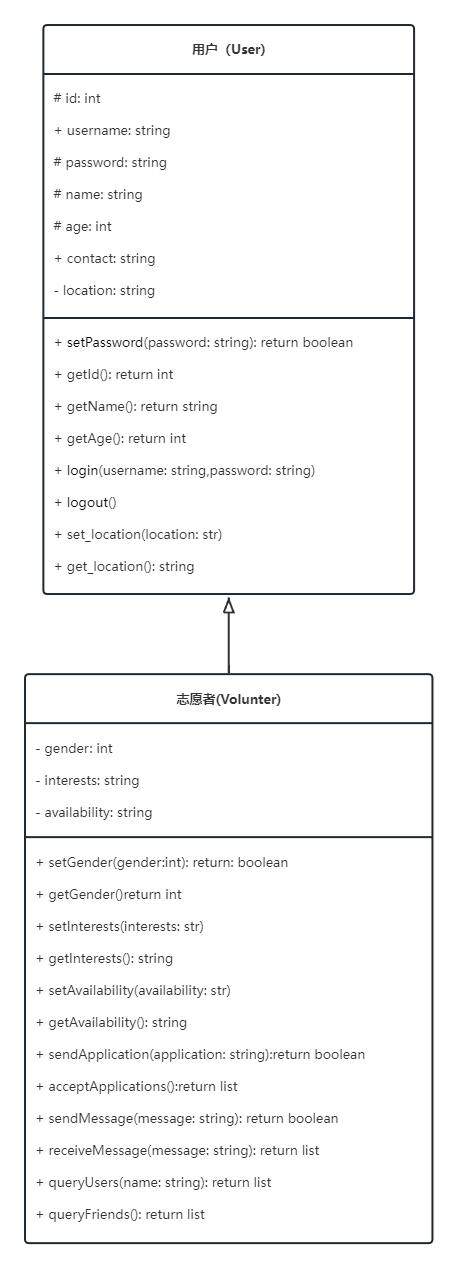
\includegraphics[scale=0.3]{OOA/fig/6-交友管理/志愿交友管理类图 (1).png}} 
    \bicaption{Volunet志愿交友系统类属性与操作1子图}{Class Attributes and Operations Sub-Diagram 1 for Volunteer Friends System of Volunet} 
\end{figure}

\begin{figure}[H] 
    \center{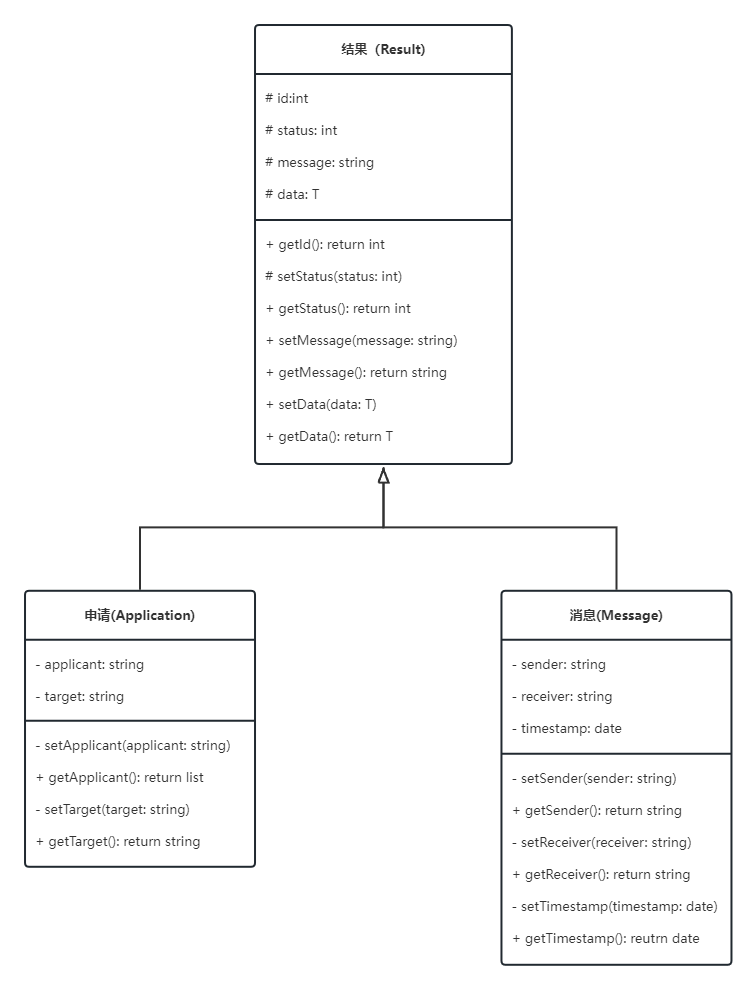
\includegraphics[scale=0.3]{OOA/fig/6-交友管理/志愿交友管理类图 (2).png}} 
    \center{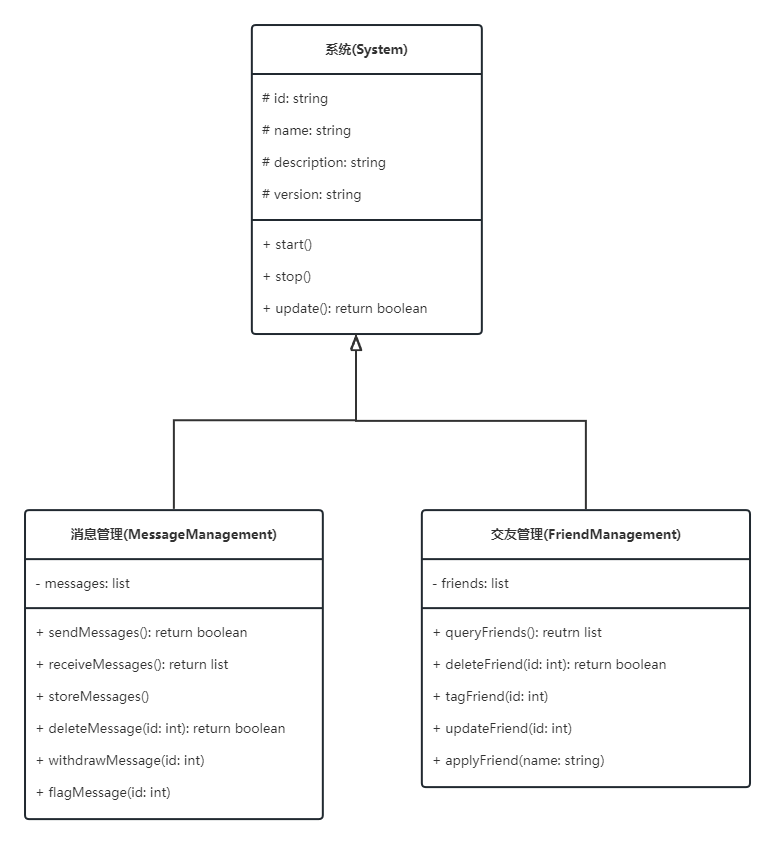
\includegraphics[scale=0.35]{OOA/fig/6-交友管理/志愿交友管理类图 (3).png}} 
    \bicaption{Volunet志愿交友系统类属性与操作2子图}{Class Attributes and Operations Sub-Diagram 2 for Volunteer Friends System of Volunet} 
\end{figure}

\paragraph{志愿交友系统类属性与操作描述}~{}

爱心捐助系统中类包含用户、志愿者、结果、申请、反馈、系统、消息管理、交友管理,它们的属性与操作描述如下:

% 用户、志愿者、结果、消息、申请、系统、交友管理系统、消息管理系统
\begin{table}[H]  
\caption{“用户”类词条描述}  
\begin{center}  
    \begin{tabular}{l p{11cm}} 
        \hline
        \quad 名称:  &  用户 \\
        \hline
        \quad 编号:  & 6.1 \\
        \hline
        \quad 英文:  &  User \\
        \hline
        \quad 简述:  & 使用交友管理系统和消息管理系统的个人的统称 \\
        \hline
        \quad 属性:  & id、username、password、name、age、contact \\
        \hline
        \quad 操作:  & setPassword()、getId()、getName()、getAge() 、login()、logout() \\
        \hline
        \quad 相关类:  & 志愿者 \\
        \hline
    \end{tabular}
\end{center}
\end{table}

\begin{table}[H]  
\caption{“志愿者”类词条描述}  
\begin{center}  
    \begin{tabular}{l p{11cm}} 
        \hline
        \quad 名称:  &  志愿者 \\
        \hline
        \quad 编号:  & 6.2 \\
        \hline
        \quad 英文:  &  Volunteer \\
        \hline
        \quad 简述:  & 使用交友管理系统和消息管理系统的个人 \\
        \hline
        \quad 属性:  & gender、interests、availability \\
        \hline 
        \quad 操作:  & setInterests()、getInterests()、setAvailability()、getAvailability()、sendApplication()、acceptApplications()、sendMessage()、receiveMessage()、queryUsers()、queryFriends()\\
        \hline
        \quad 相关类:  & 用户、交友管理系统、消息管理系统 \\
        \hline
    \end{tabular}
\end{center}
\end{table}


\begin{table}[H]  
\caption{“结果”类词条描述}  
\begin{center}  
    \begin{tabular}{l p{11cm}} 
        \hline
        \quad 名称:  &  结果 \\
        \hline
        \quad 编号:  & 6.3 \\
        \hline
        \quad 英文:  &  Result \\
        \hline
        \quad 简述:  & 完成交友管理、消息管理后所产生的输出、效果或影响 \\
        \hline
        \quad 属性:  & id、status、message、data\\
        \hline
        \quad 操作:  & getId()、setStatus()、getStatus()、setMessage()、getMessage()、setData()、getData() \\
        \hline
        \quad 相关类:  & 消息、申请 \\
        \hline
    \end{tabular}
\end{center}
\end{table}

\begin{table}[H]  
\caption{“消息”类词条描述}  
\begin{center}  
    \begin{tabular}{l p{11cm}} 
        \hline
        \quad 名称:  &  消息 \\
        \hline
        \quad 编号:  & 6.4 \\
        \hline
        \quad 英文:  &  Message \\
        \hline
        \quad 简述:  & 好友之间相互发送的文本、图像、视频信息 \\
        \hline
        \quad 属性:  & sender、receiver、timestamp \\
        \hline
        \quad 操作:  & setSender()、getSender()、setReceiver()、getReceiver()、setTimestamp()、getTimestamp()\\
        \hline
        \quad 相关类:  & 消息管理、志愿者、结果\\
        \hline
    \end{tabular}
\end{center}
\end{table}



\begin{table}[H]  
\caption{“申请”类词条描述}  
\begin{center}  
    \begin{tabular}{l p{11cm}} 
        \hline
        \quad 名称:  &  申请 \\
        \hline
        \quad 编号:  & 6.5 \\
        \hline
        \quad 英文:  &  Application \\
        \hline
        \quad 简述:  & 队其他用户请求添加好友的文件 \\
        \hline
        \quad 属性:  & applicant、target\\
        \hline
        \quad 操作:  & setApplicant()、getApplicant()、setTarget()、getTarget()\\
        \hline
        \quad 相关类:  & 志愿者、结果、交友管理 \\
        \hline
    \end{tabular}
\end{center}
\end{table}

\begin{table}[H]  
\caption{“系统”类词条描述}  
\begin{center}  
    \begin{tabular}{l p{11cm}} 
        \hline
        \quad 名称:  &  系统 \\
        \hline
        \quad 编号:  & 6.6 \\
        \hline
        \quad 英文:  &  System \\
        \hline
        \quad 简述:  & 进行管理的系统的统称 \\
        \hline
        \quad 属性:  & id、name、description、version\\
        \hline
        \quad 操作:  & start()、stop()、update()\\
        \hline
        \quad 相关类:  & 消息管理系统、交友管理系统 \\
        \hline
    \end{tabular}
\end{center}
\end{table}

\begin{table}[H]  
\caption{“交友管理系统”类词条描述}  
\begin{center}  
    \begin{tabular}{l p{11cm}} 
        \hline
        \quad 名称:  &  交友管理系统 \\
        \hline
        \quad 编号:  & 6.7 \\
        \hline
        \quad 英文:  &  FriendManagementSystem \\
        \hline
        \quad 简述:  & 负责对交友申请和用户好友进行管理和处理的系统 \\
        \hline
        \quad 属性:  & friends\\
        \hline
        \quad 操作:  & queryFriends()、deleteFriend()、tagFriend()、updateFriend()、applyFriend()\\
        \hline
        \quad 相关类:  & 系统、申请 \\
        \hline
    \end{tabular}
\end{center}
\end{table}

\begin{table}[H]  
\caption{“消息管理系统”类词条描述}  
\begin{center}  
    \begin{tabular}{l p{11cm}} 
        \hline
        \quad 名称:  &  消息管理系统 \\
        \hline
        \quad 编号:  & 6.8 \\
        \hline
        \quad 英文:  &  MessageManagementSystem \\
        \hline
        \quad 简述:  & 负责管理用户聊天消息和用户之间的消息记录的系统 \\
        \hline
        \quad 属性:  & messages\\
        \hline
        \quad 操作:  & sendMessages()、receiveMessages()、storeMessages()、deleteMessage()、withdrawMessage()、flagMessage()\\
        \hline
        \quad 相关类:  & 系统、消息 \\
        \hline
    \end{tabular}
\end{center}
\end{table}



% \subsection{交互设计}



\newpage


\fancyhead[LH]{复旦大学软件工程}
\fancyhead[RH]{第六章\quad 动态建模}
\section{动态建模}

\subsection{状态机图}
\subsubsection{信息管理系统状态机图}
\begin{figure}[H] 
    \center{
\includegraphics[scale=0.45]{OOA/fig/1-信息管理/I-状态机图1.pdf}} 
    \bicaption{Volunet信息管理系统状态机图1子图}{State Machine Sub-Diagram 1 for Information Management System of Volunet} 
\end{figure}

\begin{figure}[H] 
    \center{
\includegraphics[scale=0.4]{OOA/fig/1-信息管理/I-状态机图2.pdf}} 
    \bicaption{Volunet信息管理系统状态机图2子图}{State Machine Sub-Diagram 2 for Information Management System of Volunet} 
\end{figure}

\begin{figure}[H] 
    \center{\includegraphics[scale=0.55]{OOA/fig/1-信息管理/I-状态机图3.pdf}} 
    \bicaption{Volunet信息管理系统状态机图3子图}{State Machine Sub-Diagram 3 for Information Management System of Volunet} 
\end{figure}

\begin{figure}[H] 
    \center{\includegraphics[scale=0.55]{OOA/fig/1-信息管理/I-状态机图4.pdf}} 
    \bicaption{Volunet信息管理系统状态机图4子图}{State Machine Sub-Diagram 4 for Information Management System of Volunet} 
\end{figure}

\subsubsection{志愿服务系统状态机图}
\begin{figure}[H] 
    \center{\includegraphics[scale=0.55]{OOA/fig/2-志愿服务/VS-状态机图1.pdf}} 
    \bicaption{Volunet志愿服务系统状态机图1子图}{State Machine Sub-Diagram 1 for Voluntary Service System of Volunet} 
\end{figure}

\begin{figure}[H] 
    \center{\includegraphics[scale=0.5]{OOA/fig/2-志愿服务/VS-状态机图2.pdf}} 
    \bicaption{Volunet志愿服务系统状态机图2子图}{State Machine Sub-Diagram 2 for Voluntary Service System of Volunet} 
\end{figure}

\begin{figure}[H] 
    \center{\includegraphics[scale=0.8]{OOA/fig/2-志愿服务/VS-状态机图3.pdf}} 
    \bicaption{Volunet志愿服务系统状态机图3子图}{State Machine Sub-Diagram 3 for Voluntary Service System of Volunet} 
\end{figure}


\subsubsection{爱心捐助系统状态机图}
\begin{figure}[H] 
    \center{\includegraphics[scale=0.6]{OOA/fig/3-爱心管理/爱心管理状态机图-1.pdf}} 
    \bicaption{Volunet爱心捐助系统状态机图1子图}{State Machine Sub-Diagram 1 for Love Donation System of Volunet} 
\end{figure}

\begin{figure}[H] 
    \center{\includegraphics[scale=0.6]{OOA/fig/3-爱心管理/爱心管理状态机图-2.pdf}} 
    \bicaption{Volunet爱心捐助系统状态机图2子图}{State Machine Sub-Diagram 2 for Love Donation System of Volunet} 
\end{figure}

\begin{figure}[H] 
    \center{\includegraphics[scale=0.6]{OOA/fig/3-爱心管理/爱心管理状态机图-3.pdf}} 
    \bicaption{Volunet爱心捐助系统状态机图3子图}{State Machine Sub-Diagram 3 for Love Donation System of Volunet} 
\end{figure}

\begin{figure}[H] 
    \center{\includegraphics[scale=0.6]{OOA/fig/3-爱心管理/爱心管理状态机图-4.pdf}} 
    \bicaption{Volunet爱心捐助系统状态机图4子图}{State Machine Sub-Diagram 4 for Love Donation System of Volunet} 
\end{figure}

\subsubsection{公益课程系统状态机图}
\begin{figure}[H] 
    \center{\includegraphics[scale=0.6]{OOA/fig/4-课程管理/课程管理状态机图.png}} 
    \bicaption{Volunet公益课程系统状态机图1子图}{State Machine Sub-Diagram 1 for Course System of Volunet} 
\end{figure}

\begin{figure}[H] 
    \center{\includegraphics[scale=0.5]{OOA/fig/4-课程管理/课程管理状态机图 (1).png}} 
    \bicaption{Volunet公益课程系统状态机图2子图}{State Machine Sub-Diagram 2 for Course System of Volunet} 
\end{figure}

\begin{figure}[H] 
    \center{\includegraphics[scale=0.6]{OOA/fig/4-课程管理/课程管理状态机图 (2).png}} 
    \bicaption{Volunet公益课程系统状态机图3子图}{State Machine Sub-Diagram 3 for Course System of Volunet} 
\end{figure}

\begin{figure}[H] 
    \center{\includegraphics[scale=0.6]{OOA/fig/4-课程管理/课程管理状态机图 (3).png}} 
    \bicaption{Volunet公益课程系统状态机图4子图}{State Machine Sub-Diagram 4 for Course System of Volunet} 
\end{figure}

\subsubsection{交流论坛系统状态机图}
\begin{figure}[H] 
    \center{\includegraphics[scale=0.85]{OOA/fig/5-论坛管理/论坛管理资讯信息对象状态机图.pdf}} 
    \bicaption{Volunet交流论坛系统资讯信息对象的状态机图}{State Machine Sub-Diagram Of News Information Object for Communication System of Volunet} 
\end{figure}

\begin{figure}[H] 
    \center{\includegraphics[scale=0.85]{OOA/fig/5-论坛管理/论坛管理资讯类型对象状态机图.pdf}}
     \bicaption{Volunet交流论坛系统资讯类别对象的状态机图}{State Machine Sub-Diagram Of News Category Information Object for Communication System of Volunet} 
\end{figure}

\begin{figure}[H] 
    \center{\includegraphics[scale=0.85]{OOA/fig/5-论坛管理/论坛管理资讯评论对象状态机.pdf}} 
     \bicaption{Volunet交流论坛系统资讯评论对象的状态机图}{State Machine Sub-Diagram Of News Comment Information Object for Communication System of Volunet} 
\end{figure}

\begin{figure}[H] 
    \center{\includegraphics[scale=0.85]{OOA/fig/5-论坛管理/论坛管理手记信息对象状态机图.pdf}} 
     \bicaption{Volunet交流论坛系统手记信息对象的状态机图}{State Machine Sub-Diagram Of Journal Information Object for Communication System of Volunet} 
\end{figure}

\begin{figure}[H] 
    \center{\includegraphics[scale=0.85]{OOA/fig/5-论坛管理/论坛管理手记评论对象状态图.pdf}} 
     \bicaption{Volunet交流论坛系统手机评论对象的状态机图}{State Machine Sub-Diagram Of Journal Comment Object for Communication System of Volunet} 
\end{figure}

\begin{figure}[H] 
    \center{\includegraphics[scale=0.85]{OOA/fig/5-论坛管理/论坛管理帖子信息对象状态机图.pdf}} 
     \bicaption{Volunet交流论坛系统帖子信息对象的状态机图}{State Machine Sub-Diagram Of Post Information Object for Communication System of Volunet} 
\end{figure}

\begin{figure}[H] 
    \center{\includegraphics[scale=0.85]{OOA/fig/5-论坛管理/论坛管理论坛版块对象状态机图.pdf}} 
     \bicaption{Volunet交流论坛系统板块信息对象的状态机图}{State Machine Sub-Diagram Of Section Information Object for Communication System of Volunet} 
\end{figure}

\begin{figure}[H] 
    \center{\includegraphics[scale=0.85]{OOA/fig/5-论坛管理/论坛管理审计报表对象状态机图.pdf}} 
     \bicaption{Volunet交流论坛系统审计报表对象的状态机图}{State Machine Sub-Diagram Of Audition Report Object for Communication System of Volunet} 
\end{figure}

\subsubsection{志愿交友系统状态机图}
\begin{figure}[H] 
    \center{\includegraphics[scale=0.6]{OOA/fig/6-交友管理/志愿交友管理状态机图.png}} 
    \bicaption{Volunet志愿交友系统状态机图1子图}{State Machine Sub-Diagram 1 for Volunteer Friends System of Volunet} 
\end{figure}

\begin{figure}[H] 
    \center{\includegraphics[scale=0.6]{OOA/fig/6-交友管理/志愿交友管理状态机图 (1).png}} 
    \bicaption{Volunet志愿交友系统状态机图2子图}{State Machine Sub-Diagram 2 for Volunteer Friends System of Volunet} 
\end{figure}

\quad
\subsection{活动图}
\subsubsection{信息管理系统活动图}
\begin{figure}[H] 
    \center{\includegraphics[scale=0.9]{OOA/fig/1-信息管理/I-活动图1.pdf}} 
    \bicaption{Volunet信息管理系统活动1子图}{Activity Sub-Diagram 1 for Information Management System of Volunet} 
\end{figure}

\begin{figure}[H] 
    \center{\includegraphics[scale=0.9]{OOA/fig/1-信息管理/I-活动图2.pdf}} 
    \bicaption{Volunet信息管理系统活动2子图}{Activity Sub-Diagram 2 for Information Management System of Volunet} 
\end{figure}

\begin{figure}[H] 
    \center{\includegraphics[scale=1.2]{OOA/fig/1-信息管理/I-活动图3.pdf}} 
    \bicaption{Volunet信息管理系统活动3子图}{Activity Sub-Diagram 3 for Information Management System of Volunet} 
\end{figure}

\subsubsection{志愿服务系统活动图}
\begin{figure}[H] 
    \center{\includegraphics[scale=0.9]{OOA/fig/2-志愿服务/VS-活动图1.pdf}} 
    \bicaption{Volunet志愿服务系统活动1子图}{Activity Sub-Diagram 1 for Voluntary Service System of Volunet} 
\end{figure}

\begin{figure}[H] 
    \center{\includegraphics[scale=0.6]{OOA/fig/2-志愿服务/VS-活动图2.pdf}} 
    \bicaption{Volunet志愿服务系统活动2子图}{Activity Sub-Diagram 2 for Voluntary Service System of Volunet} 
\end{figure}

\begin{figure}[H] 
    \center{\includegraphics[scale=0.6]{OOA/fig/2-志愿服务/VS-活动图3.pdf}} 
    \bicaption{Volunet志愿服务系统活动3子图}{Activity Sub-Diagram 3 for Voluntary Service System of Volunet} 
\end{figure}


\subsubsection{爱心捐助系统活动图}
\begin{figure}[H] 
    \center{\includegraphics[scale=0.7]{OOA/fig/3-爱心管理/爱心管理活动图-1.pdf}} 
    \bicaption{Volunet爱心捐助系统活动1子图}{Activity Sub-Diagram 1 for Love Donation System of Volunet} 
\end{figure}

\begin{figure}[H] 
    \center{\includegraphics[scale=0.6]{OOA/fig/3-爱心管理/爱心管理活动图-2.pdf}} 
    \bicaption{Volunet爱心捐助系统活动2子图}{Activity Sub-Diagram 2 for Love Donation System of Volunet} 
\end{figure}

\begin{figure}[H] 
    \center{\includegraphics[scale=0.6]{OOA/fig/3-爱心管理/爱心管理活动图-3.pdf}} 
    \bicaption{Volunet爱心捐助系统活动3子图}{Activity Sub-Diagram 3 for Love Donation System of Volunet} 
\end{figure}

\subsubsection{公益课程系统活动图}
\begin{figure}[H] 
    \center{\includegraphics[scale=0.3]{OOA/fig/4-课程管理/课程管理活动图.png}} 
    \bicaption{Volunet公益课程系统活动1子图}{Activity Sub-Diagram 1 for Course System of Volunet} 
\end{figure}

\begin{figure}[H] 
    \center{\includegraphics[scale=0.35]{OOA/fig/4-课程管理/课程管理活动图 (1).png}} 
    \bicaption{Volunet公益课程系统活动2子图}{Activity Sub-Diagram 2 for Course System of Volunet} 
\end{figure}

\begin{figure}[H] 
    \center{\includegraphics[scale=0.35]{OOA/fig/4-课程管理/课程管理活动图 (2).png}} 
    \bicaption{Volunet公益课程系统活动3子图}{Activity Sub-Diagram 3 for Course System of Volunet} 
\end{figure}

\subsubsection{交流论坛系统活动图}
\begin{figure}[H] 
    \center{\includegraphics[scale=0.55]{OOA/fig/5-论坛管理/论坛管理资讯信息对象活动图.pdf}} 
    \bicaption{Volunet交流论坛系统资讯信息活动图}{Activity Sub-Diagram Of News Information Object for Communication System of Volunet} 
\end{figure}

\begin{figure}[H] 
    \center{\includegraphics[scale=0.55]{OOA/fig/5-论坛管理/论坛管理资讯类型对象活动图.pdf}} 
    \bicaption{Volunet交流论坛系统资讯类型活动图}{Activity Sub-Diagram Of News Category Object for Communication System of Volunet} 
\end{figure}

\begin{figure}[H] 
    \center{\includegraphics[scale=0.55]{OOA/fig/5-论坛管理/论坛管理资讯评论对象活动图.pdf}} 
    \bicaption{Volunet交流论坛系统资讯评论活动图}{Activity Sub-Diagram Of News Comment Object for Communication System of Volunet} 
\end{figure}

\begin{figure}[H] 
    \center{\includegraphics[scale=0.55]{OOA/fig/5-论坛管理/论坛管理手记信息对象活动图 .pdf}} 
    \bicaption{Volunet交流论坛系统手记信息活动图}{Activity Sub-Diagram Of Journal Information Object for Communication System of Volunet} 
\end{figure}

\begin{figure}[H] 
    \center{\includegraphics[scale=0.55]{OOA/fig/5-论坛管理/论坛管理手记评论对象活动图.pdf}} 
    \bicaption{Volunet交流论坛系统手记评论活动图}{Activity Sub-Diagram Of Journal Comment Object for Communication System of Volunet} 
\end{figure}

\begin{figure}[H] 
    \center{\includegraphics[scale=0.55]{OOA/fig/5-论坛管理/论坛管理帖子信息对象活动图.pdf}} 
    \bicaption{Volunet交流论坛系统帖子信息活动1子图}{Activity Sub-Diagram 1 Of Post Information Object for Communication System of Volunet} 
\end{figure}

\begin{figure}[H] 
    \center{\includegraphics[scale=0.55]{OOA/fig/5-论坛管理/论坛管理帖子信息对象活动图-2.pdf}} 
    \bicaption{Volunet交流论坛系统帖子信息活动2子图}{Activity Sub-Diagram 2 Of Post Information Object for Communication System of Volunet} 
\end{figure}

\begin{figure}[H] 
    \center{\includegraphics[scale=0.55]{OOA/fig/5-论坛管理/论坛管理板块信息对象活动图.pdf}} 
    \bicaption{Volunet交流论坛版块信息活动图}{Activity Sub-Diagram Of Section Information Object for Communication System of Volunet} 
\end{figure}

\begin{figure}[H] 
    \center{\includegraphics[scale=0.8]{OOA/fig/5-论坛管理/论坛管理审计报表对象活动图.pdf}} 
    \bicaption{Volunet交流论坛审计报表活动图}{Activity Sub-Diagram Of Audition Report Object for Communication System of Volunet} 
\end{figure}

\subsubsection{志愿交友系统活动图}
\begin{figure}[H] 
    \center{\includegraphics[scale=0.3]{OOA/fig/6-交友管理/志愿交友管理活动图.png}} 
    \bicaption{Volunet志愿交友系统活动1子图}{Activity Sub-Diagram 1 for Volunteer Friends System of Volunet} 
\end{figure}

\begin{figure}[H] 
    \center{\includegraphics[scale=0.4]{OOA/fig/6-交友管理/志愿交友管理活动图 (1).png}} 
    \bicaption{Volunet志愿交友系统活动2子图}{Activity Sub-Diagram 2 for Volunteer Friends System of Volunet} 
\end{figure}

\subsection{顺序图}

\subsubsection{信息管理系统顺序图}
\begin{figure}[H] 
    \center{\includegraphics[scale=0.65]{OOA/fig/1-信息管理/I-顺序图1.pdf}} 
    \bicaption{Volunet信息管理系统顺序1子图}{Sequence Sub-Diagram 1 for Information Management System of Volunet} 
\end{figure}

\begin{figure}[H] 
    \center{\includegraphics[scale=0.65]{OOA/fig/1-信息管理/I-顺序图2.pdf}} 
    \bicaption{Volunet信息管理系统顺序2子图}{Sequence Sub-Diagram 2 for Information Management System of Volunet} 
\end{figure}

\begin{figure}[H] 
    \center{\includegraphics[scale=0.6]{OOA/fig/1-信息管理/I-顺序图3.pdf}} 
    \bicaption{Volunet信息管理系统顺序3子图}{Sequence Sub-Diagram 3 for Information Management System of Volunet} 
\end{figure}

\begin{figure}[H] 
    \center{\includegraphics[scale=0.6]{OOA/fig/1-信息管理/I-顺序图4.pdf}} 
    \bicaption{Volunet信息管理系统顺序4子图}{Sequence Sub-Diagram 4 for Information Management System of Volunet} 
\end{figure}

\subsubsection{志愿服务系统顺序图}
\begin{figure}[H] 
    \center{\includegraphics[scale=0.65]{OOA/fig/2-志愿服务/VS-顺序图1.pdf}} 
    \bicaption{Volunet志愿服务系统顺序1子图}{Sequence Sub-Diagram 1 for Voluntary Service System of Volunet} 
\end{figure}

\begin{figure}[H] 
    \center{\includegraphics[scale=0.6]{OOA/fig/2-志愿服务/VS-顺序图2.pdf}} 
    \bicaption{Volunet志愿服务系统顺序2子图}{Sequence Sub-Diagram 2 for Voluntary Service System of Volunet} 
\end{figure}

\begin{figure}[H] 
    \center{\includegraphics[scale=0.6]{OOA/fig/2-志愿服务/VS-顺序图3.pdf}} 
    \bicaption{Volunet志愿服务系统顺序3子图}{Sequence Sub-Diagram 3 for Voluntary Service System of Volunet} 
\end{figure}

\subsubsection{爱心捐助系统顺序图}
\begin{figure}[H] 
    \center{\includegraphics[scale=0.5]{OOA/fig/3-爱心管理/爱心管理顺序图-1.pdf}} 
    \bicaption{Volunet爱心捐助系统顺序1子图}{Sequence Sub-Diagram 1 for Love Donation System of Volunet} 
\end{figure}

\begin{figure}[H] 
    \center{\includegraphics[scale=0.6]{OOA/fig/3-爱心管理/爱心管理顺序图-2.pdf}} 
    \bicaption{Volunet爱心捐助系统顺序2子图}{Sequence Sub-Diagram 2 for Love Donation System of Volunet} 
\end{figure}

\begin{figure}[H] 
    \center{\includegraphics[scale=0.6]{OOA/fig/3-爱心管理/爱心管理顺序图-3.pdf}} 
    \bicaption{Volunet爱心捐助系统顺序3子图}{Sequence Sub-Diagram 3 for Love Donation System of Volunet} 
\end{figure}

\subsubsection{公益课程系统顺序图}
\begin{figure}[H] 
    \center{\includegraphics[scale=0.2]{OOA/fig/4-课程管理/课程管理顺序图.png}} 
    \bicaption{Volunet公益课程系统顺序1子图}{Sequence Sub-Diagram 1 for Course System of Volunet} 
\end{figure}

\begin{figure}[H] 
    \center{\includegraphics[scale=0.35]{OOA/fig/4-课程管理/课程管理顺序图 (1).png}} 
    \bicaption{Volunet公益课程系统顺序2子图}{Sequence Sub-Diagram 2 for Course System of Volunet} 
\end{figure}

\begin{figure}[H] 
    \center{\includegraphics[scale=0.3]{OOA/fig/4-课程管理/课程管理顺序图 (2).png}} 
    \bicaption{Volunet公益课程系统顺序3子图}{Sequence Sub-Diagram 3 for Course System of Volunet} 
\end{figure}

\subsubsection{交流论坛系统顺序图}
\begin{figure}[H] 
    \center{\includegraphics[scale=0.38]{OOA/fig/5-论坛管理/论坛管理资讯管理顺序图.pdf}} 
    \bicaption{Volunet交流论坛系统咨询管理顺序图}{Sequence Diagram Of News Management for Communication  System of Volunet} 
\end{figure}

\begin{figure}[H] 
    \center{\includegraphics[scale=0.5]{OOA/fig/5-论坛管理/论坛管理手记管理顺序图.pdf}} 
    \bicaption{Volunet交流论坛系统手记管理顺序图}{Sequence Diagram Of Journal Management for Communication  System of Volunet} 
\end{figure}

\begin{figure}[H] 
    \center{\includegraphics[scale=0.45]{OOA/fig/5-论坛管理/论坛管理论坛管理顺序图.pdf}} 
    \bicaption{Volunet交流论坛系统论坛管理顺序图}{Sequence Diagram Of Fourm Management for Communication  System of Volunet} 
\end{figure}

\subsubsection{志愿交友系统顺序图}
\begin{figure}[H] 
    \center{\includegraphics[scale=0.3]{OOA/fig/6-交友管理/志愿交友管理顺序图.png}} 
    \bicaption{Volunet志愿交友系统顺序1子图}{Sequence Sub-Diagram 1 for Volunteer Friends System of Volunet} 
\end{figure}

\begin{figure}[H] 
    \center{\includegraphics[scale=0.4]{OOA/fig/6-交友管理/志愿交友管理顺序图 (1).png}} 
    \bicaption{Volunet志愿交友系统顺序2子图}{Sequence Sub-Diagram 2 for Volunteer Friends System of Volunet} 
\end{figure}

\subsection{通信图}
\subsubsection{信息管理系统通信图}
\begin{figure}[H] 
    \center{\includegraphics[scale=0.65]{OOA/fig/1-信息管理/I-通信图.pdf}} 
    \bicaption{Volunet信息管理系统通信图}{Communication Diagram for Information Management System of Volunet} 
\end{figure}


\subsubsection{志愿服务系统通信图}
\begin{figure}[H] 
    \center{\includegraphics[scale=0.60, angle=90]{OOA/fig/2-志愿服务/VS-通信图.pdf}} 
    \bicaption{Volunet志愿服务系统通信图}{Communication Diagram for Voluntary Service System of Volunet} 
\end{figure}

\subsubsection{爱心捐助系统通信图}
\begin{figure}[H] 
    \center{\includegraphics[scale=0.47]{OOA/fig/3-爱心管理/爱心管理通信图.pdf}} 
    \bicaption{Volunet爱心捐助系统通信图}{Communication Diagram for Love Donation System of Volunet} 
\end{figure}

\subsubsection{公益课程系统通信图}
\begin{figure}[H] 
    \center{\includegraphics[scale=0.3]{OOA/fig/4-课程管理/课程管理通信图.png}} 
    \bicaption{Volunet公益课程系统通信图}{Communication Diagram for Course System of Volunet} 
\end{figure}

\subsubsection{交流论坛系统通信图}
\begin{figure}[H] 
    \center{\includegraphics[scale=0.4, angle=90]{OOA/fig/5-论坛管理/论坛管理通信图.pdf}} 
    \bicaption{Volunet交流论坛系统通信图}{Communication Diagram for Communication System of Volunet} 
\end{figure}

\subsubsection{志愿交友系统通信图}
\begin{figure}[H] 
    \center{\includegraphics[scale=0.47]{OOA/fig/6-交友管理/志愿交友管理通信图.png}} 
    \bicaption{Volunet志愿交友系统通信图}{Communication Diagram for Volunteer Friends System of Volunet} 
\end{figure}

% \newpage

\fancyhead[LH]{复旦大学软件工程}
\fancyhead[RH]{第七章\quad 物理体系结构建模}

\section{物理体系结构建模}

% \subsection{物理体系结构建模}

\subsection{包图}

% \subsubsection{总体功能包图}
\subsubsection{信息管理系统包图}

\begin{figure}[H] 
    \center{\includegraphics[scale=0.25]{OOA/fig/1-信息管理/信息管理包图.pdf}} 
    \bicaption{Volunet信息管理系统包图}{Package Diagram for Information Management System of Volunet} 
\end{figure}

\subsubsection{志愿服务系统包图}

\begin{figure}[H] 
    \center{\includegraphics[scale=0.54]{OOA/fig/2-志愿服务/VS-包图.pdf}} 
    \bicaption{Volunet志愿服务系统包图}{Package Diagram for Voluntary Service System of Volunet} 
\end{figure}
\quad
\subsubsection{爱心捐助系统包图}
\begin{figure}[H] 
    \center{\includegraphics[scale=0.38]{OOA/fig/3-爱心管理/爱心捐助包图.pdf}} 
    \bicaption{Volunet爱心捐助系统包图}{Package Diagram for Love Donation System of Volunet} 
\end{figure}

\subsubsection{公益课程系统包图}
\begin{figure}[H] 
    \center{\includegraphics[scale=0.25]{OOA/fig/4-课程管理/课程管理包图.png}} 
    \bicaption{Volunet公益课程系统包图}{Package Diagram for Course System of Volunet} 
\end{figure}

\subsubsection{交流论坛系统包图}
\begin{figure}[H] 
    \center{\includegraphics[scale=0.3]{OOA/fig/5-论坛管理/论坛管理包图.pdf}} 
    \bicaption{Volunet交流论坛系统包图}{Package Diagram for Communication System of Volunet} 
\end{figure}

\subsubsection{志愿交友系统包图}
\begin{figure}[H] 
    \center{\includegraphics[scale=0.35]{OOA/fig/6-交友管理/志愿交友管理包图.png}} 
    \bicaption{Volunet志愿交友系统包图}{Package Diagram for Volunteer Friends System of Volunet} 
\end{figure}

\subsection{构件图}

\subsubsection{信息管理系统构件图}
\begin{figure}[H] 
    \center{\includegraphics[scale=0.67]{OOA/fig/1-信息管理/信息管理构件图.pdf}} 
    \bicaption{Volunet信息管理系统构件图}{Component Diagram for Information Management System of Volunet} 
\end{figure}

\subsubsection{志愿服务系统构件图}
\begin{figure}[H] 
    \center{\includegraphics[scale=0.60]{OOA/fig/2-志愿服务/VS-构件图.pdf}} 
    \bicaption{Volunet志愿服务系统构件图}{Component Diagram for Voluntary Service System of Volunet} 
\end{figure}

%\quad
\subsubsection{爱心捐助系统构件图}
\begin{figure}[H] 
    \center{\includegraphics[scale=0.52]{OOA/fig/3-爱心管理/爱心捐助构件图.pdf}} 
    \bicaption{Volunet爱心捐助系统构件图}{Component Diagram for Love Donation System of Volunet} 
\end{figure}
\quad

\subsubsection{公益课程系统构件图}
\begin{figure}[H] 
    \center{\includegraphics[scale=0.3]{OOA/fig/4-课程管理/课程管理构件图.png}} 
    \bicaption{Volunet公益课程系统构件图}{Component Diagram for Course System of Volunet} 
\end{figure}


\subsubsection{交流论坛系统构件图}
\begin{figure}[H] 
    \center{\includegraphics[scale=0.55, angle=90]{OOA/fig/5-论坛管理/论坛管理构件图.pdf}} 
    \bicaption{Volunet交流论坛系统构件图}{Component Diagram for Communication System of Volunet} 
\end{figure}
\quad

\subsubsection{志愿交友系统构件图}
\begin{figure}[H] 
    \center{\includegraphics[scale=0.4, angle=90]{OOA/fig/6-交友管理/志愿交友管理构件图.png}} 
    \bicaption{Volunet志愿交友系统构件图}{Component Diagram for Volunteer Friends System of Volunet} 
\end{figure}

\subsection{部署图}
 
\subsubsection{信息管理系统部署图}

\begin{figure}[H] 
    \center{\includegraphics[scale=0.35]{OOA/fig/1-信息管理/信息管理部署图.pdf}} 
    \bicaption{Volunet信息管理系统部署图}{Deployment Diagram for Information Management System of Volunet} 
\end{figure}

\subsubsection{志愿服务系统部署图}
\begin{figure}[H] 
    \center{\includegraphics[scale=0.45, angle=90]{OOA/fig/2-志愿服务/VS-部署图.pdf}} 
    \bicaption{Volunet信息管理系统部署图}{Deployment Diagram for Voluntary Service System of Volunet} 
\end{figure}

\subsubsection{爱心捐助系统部署图}
\begin{figure}[H] 
    \center{\includegraphics[scale=0.4]{OOA/fig/3-爱心管理/爱心捐助部署图.pdf}} 
    \bicaption{Volunet爱心捐助系统部署图}{Deployment Diagram for Love Donation System of Volunet} 
\end{figure}

\subsubsection{公益课程系统部署图}
\begin{figure}[H] 
    \center{\includegraphics[scale=0.17]{OOA/fig/4-课程管理/课程管理部署图.png}} 
    \bicaption{Volunet公益课程系统部署图}{Deployment Diagram for Course System of Volunet} 
\end{figure}

\subsubsection{交流论坛系统部署图}
\begin{figure}[H] 
    \center{\includegraphics[scale=0.35, angle=90]{OOA/fig/5-论坛管理/论坛管理部署图.pdf}} 
    \bicaption{Volunet交流论坛系统部署图}{Deployment Diagram for Communication System of Volunet} 
\end{figure}
\quad

\subsubsection{志愿交友系统部署图}
\begin{figure}[H] 
    \center{\includegraphics[scale=0.35, angle=90]{OOA/fig/6-交友管理/志愿交友管理部署图.png}} 
    \bicaption{Volunet志愿交友系统部署图}{Deployment Diagram for Communication Volunteer Friends of Volunet} 
\end{figure}

\newpage

\fancyhead[LH]{复旦大学软件工程}
\fancyhead[RH]{第八章\quad 检验与测试}
\section{检验与测试}

\subsection{测试说明}
\subsubsection{测试目的}
\begin{itemize}[itemsep=2pt,topsep=0pt,parsep=4pt,itemindent=1em]
    \item 确定测试阶段的管理工作和技术工作提供参考,包括测试计划、测试用例、测试执行和测试报告等,以确保测试工作有序进行,测试结果可靠。
    \item 确定测试的内容和范围,包括系统功能测试、性能测试、安全测试、用户体验测试和兼容性测试,以覆盖系统的各个方面,发现潜在问题并及时解决。
    \item 为volunet志愿服务系统的评价提供依据和指标,包括用户注册、发布任务、接受任务、完成任务等功能的可用性、响应时间、并发用户数、数据处理速度、用户数据的保护、防止恶意攻击、防止数据泄露等安全性指标、界面设计、易用性、用户反馈等用户体验指标,以评估系统的优劣和提出改进建议。
    \item 发现系统的潜在问题并及时解决,提高系统的稳定性和用户体验,为用户提供更好的志愿服务体验。
\end{itemize}

\subsubsection{测试方针}
\begin{itemize}[itemsep=2pt,topsep=0pt,parsep=4pt,itemindent=1em]
    \item \textbf{测试目标:} 测试目标是发现系统的潜在问题并提供改进建议,以确保系统的稳定性和用户体验。
    \item \textbf{测试范围:} 测试范围包括系统功能测试、性能测试、安全测试、用户体验测试和兼容性测试,以覆盖系统的各个方面。
    \item \textbf{测试策略:} 测试策略是基于风险的测试,根据系统的重要性和影响程度,优先测试高风险区域和关键功能。
    \item \textbf{测试方法:} 测试方法包括手动测试和自动化测试,手动测试用于测试系统的人机交互和用户体验,自动化测试用于测试系统的功能和性能。
    \item \textbf{测试用例:} 测试用例是测试的基本单位,测试用例应该覆盖所有功能和场景,以确保系统的完整性和正确性。
    \item \textbf{测试数据:} 测试数据应该包括各种类型的数据,包括正常数据、异常数据、边界数据等,以确保系统的可靠性和鲁棒性。
    \item \textbf{测试环境:} 测试环境应该与生产环境相同或接近,以确保测试结果的可靠性和准确性。
    \item \textbf{测试报告:} 测试报告应该包括测试结果、测试覆盖率、测试缺陷和改进建议等,以便开发人员和项目管理人员了解测试进展和测试结果。
    \item \textbf{测试人员:} 测试人员应该具备专业的测试技能和知识,熟悉测试流程和测试工具,以确保测试的有效性和准确性。
\end{itemize}

\\

通过以上测试方针,可以确保测试工作的有效性和完整性,发现系统的潜在问题并及时解决,提高系统的稳定性和用户体验,为用户提供更好的志愿服务体验。
\subsection{功能测试}
\subsubsection{功能性测试说明}
\begin{itemize}[itemsep=2pt,topsep=0pt,parsep=4pt,itemindent=1em]
 \item \textbf{明确目标:} 测试应该有明确的目标和预期结果,以便能够确定测试是否成功。

\item \textbf{重要性:} 测试应该重点测试最重要的功能,以确保系统的核心功能正常工作。

\item \textbf{可重复性:} 功能性测试应该是可重复的,以便能够在需要时重复执行相同的测试,并获得相同的结果。

\item \textbf{可自动化:} 功能性测试应该是可自动化的,以便能够快速、准确地执行测试,并节省时间和资源。

\item \textbf{完整性:} 测试应该覆盖所有的功能,以确保系统的完整性。

\item \textbf{可测量:} 功能性测试应该是可测量的,以便能够确定测试的成功和失败。

\item \textbf{可维护性:} 功能性测试应该是可维护的,以便能够在系统更新后对测试进行更新和修改。

\item \textbf{可扩展性:} 功能性测试应该是可扩展的,以便能够在需要时添加新的测试用例。

\item \textbf{可靠性:} 功能性测试应该是可靠的,以便能够获得准确和可信的测试结果。

\item \textbf{可重构性:} 功能性测试应该是可重构的,以便能够在需要时对测试进行重构和改进。
\end{itemize}\\

限于篇幅,下面仅列出部分高优先级的功能性测试用例。

\subsubsection{部分功能性测试样例}
\begin{framed} \textbf{测试用例编号:} TC-A001

\textbf{测试模块:} 用户注册

\textbf{测试标题:} 注册新用户

\textbf{重要级别:} 高

\textbf{预置条件:} 无

\textbf{输入数据:} 用户名、密码、电子邮件地址

\textbf{预期输出:} 成功创建新用户并显示成功消息

\begin{center} \fbox{\parbox{0.8\textwidth}{TC-A001测试结果: 通过}} \end{center} \end{framed}

\begin{framed} \textbf{测试用例编号:} TC-A002

\textbf{测试模块:} 用户登录

\textbf{测试标题:} 使用正确的用户名和密码登录

\textbf{重要级别:} 高

\textbf{预置条件:} 已注册用户

\textbf{输入数据:} 用户名、密码

\textbf{预期输出:} 成功登录并显示欢迎消息

\begin{center} \fbox{\parbox{0.8\textwidth}{TC-A002测试结果: 通过}} \end{center} \end{framed}

\begin{framed} \textbf{测试用例编号:} TC-A003

\textbf{测试模块:} 用户登录

\textbf{测试标题:} 使用错误的用户名和密码登录

\textbf{重要级别:} 中

\textbf{预置条件:} 已注册用户

\textbf{输入数据:} 错误的用户名、密码

\textbf{预期输出:} 登录失败并显示错误消息

\begin{center} \fbox{\parbox{0.8\textwidth}{TC-A003测试结果: 通过}} \end{center} \end{framed}

\begin{framed} \textbf{测试用例编号:} TC-A004

\textbf{测试模块:} 用户管理

\textbf{测试标题:} 查看用户列表

\textbf{重要级别:} 中

\textbf{预置条件:} 已登录管理员账户

\textbf{输入数据:} 点击用户管理菜单

\textbf{预期输出:} 显示所有用户的列表

\begin{center} \fbox{\parbox{0.8\textwidth}{TC-A004测试结果: 通过}} \end{center} \end{framed}

\begin{framed} \textbf{测试用例编号:} TC-A005

\textbf{测试模块:} 用户管理

\textbf{测试标题:} 编辑用户信息

\textbf{重要级别:} 高

\textbf{预置条件:} 已登录管理员账户

\textbf{输入数据:} 选择一个用户并编辑他的信息

\textbf{预期输出:} 成功更新用户信息并显示成功消息

\begin{center} \fbox{\parbox{0.8\textwidth}{TC-A005测试结果: 通过}} \end{center} \end{framed}

\begin{framed} \textbf{测试用例编号:} TC-A006

\textbf{测试模块:} 用户管理

\textbf{测试标题:} 删除用户

\textbf{重要级别:} 高

\textbf{预置条件:} 已登录管理员账户

\textbf{输入数据:} 选择一个用户并删除他

\textbf{预期输出:} 成功删除用户并显示成功消息

\begin{center} \fbox{\parbox{0.8\textwidth}{TC-A006测试结果: 通过}} \end{center} \end{framed}

\begin{framed} \textbf{测试用例编号:} TC-A007

\textbf{测试模块:} 任务管理

\textbf{测试标题:} 创建任务

\textbf{重要级别:} 高

\textbf{预置条件:} 已登录管理员账户

\textbf{输入数据:} 任务标题、描述、截止日期等信息

\textbf{预期输出:} 成功创建任务并显示成功消息

\begin{center} \fbox{\parbox{0.8\textwidth}{TC-A007测试结果: 通过}} \end{center} \end{framed}

\begin{framed} \textbf{测试用例编号:} TC-A008

\textbf{测试模块:} 任务管理

\textbf{测试标题:} 查看任务列表

\textbf{重要级别:} 中

\textbf{预置条件:} 已登录用户账户

\textbf{输入数据:} 点击任务列表菜单

\textbf{预期输出:} 显示所有任务的列表

\begin{center} \fbox{\parbox{0.8\textwidth}{TC-A008测试结果: 通过}} \end{center} \end{framed}

\begin{framed} \textbf{测试用例编号:} TC-A009

\textbf{测试模块:} 活动发布

\textbf{测试标题:} 发布活动

\textbf{重要级别:} 高

\textbf{预置条件:} 用户已登录

\textbf{输入数据:} 活动名称、活动时间、活动地点、活动描述、招募人数

\textbf{预期输出:} 活动发布成功,并显示在活动列表中

\begin{center} \fbox{\parbox{0.8\textwidth}{TC-A009测试结果: 通过}} \end{center} \end{framed}

\begin{framed} \textbf{测试用例编号:} TC-A010

\textbf{测试模块:} 活动管理

\textbf{测试标题:} 修改活动

\textbf{重要级别:} 高

\textbf{预置条件:} 用户已登录,已发布一项活动

\textbf{输入数据:} 修改后的活动名称、活动时间、活动地点、活动描述、招募人数

\textbf{预期输出:} 活动信息更新成功,并显示在活动列表中

\begin{center} \fbox{\parbox{0.8\textwidth}{TC-A010测试结果: 通过}} \end{center} \end{framed}

\begin{framed} \textbf{测试用例编号:} TC-A011

\textbf{测试模块:} 活动管理

\textbf{测试标题:} 删除活动

\textbf{重要级别:} 高

\textbf{预置条件:} 用户已登录,已发布一项活动

\textbf{输入数据:} 删除该活动

\textbf{预期输出:} 活动信息删除成功,并不再显示在活动列表中

\begin{center} \fbox{\parbox{0.8\textwidth}{TC-A011测试结果: 通过}} \end{center} \end{framed}

\begin{framed} \textbf{测试用例编号:} TC-A012

\textbf{测试模块:} 入队管理

\textbf{测试标题:} 申请参加活动

\textbf{重要级别:} 高

\textbf{预置条件:} 用户已登录,已有一项活动发布

\textbf{输入数据:} 申请参加该活动

\textbf{预期输出:} 申请信息提交成功,并等待活动发布者审核

\begin{center} \fbox{\parbox{0.8\textwidth}{TC-A012测试结果: 通过}} \end{center} \end{framed}

\begin{framed} \textbf{测试用例编号:} TC-A013

\textbf{测试模块:} 活动管理

\textbf{测试标题:} 审核志愿者申请

\textbf{重要级别:} 高

\textbf{预置条件:} 用户已登录,已有一项待审核的志愿者申请

\textbf{输入数据:} 审核该志愿者申请,同意或拒绝

\textbf{预期输出:} 志愿者申请审核结果提交成功,并通知申请者审核结果

\begin{center} \fbox{\parbox{0.8\textwidth}{TC-A013测试结果: 通过}} \end{center} \end{framed}

\begin{framed} \textbf{测试用例编号:} TC-A014

\textbf{测试模块:} 活动管理

\textbf{测试标题:} 筛选活动

\textbf{重要级别:} 中

\textbf{预置条件:} 用户已登录,已发布多项活动

\textbf{输入数据:} 活动名称、活动时间、活动地点、招募人数等筛选条件

\textbf{预期输出:} 显示符合筛选条件的活动列表

\begin{center} \fbox{\parbox{0.8\textwidth}{TC-A014测试结果: 通过}} \end{center} \end{framed}
\subsubsection{测试通过条件}
\begin{itemize}[itemsep=2pt,topsep=0pt,parsep=4pt,itemindent=1em]
\item \textbf{错误率:}系统在给定输入的情况下,能够以较低的错误率通过所有的测试样例与场景。对于重要的功能,系统的错误率必须控制在极低的水平。例如,系统应该能够准确地将任务分配给正确的志愿者,确保任务的及时完成和质量。此外,系统应该能够确保志愿者和组织之间的所有通信都能够及时、准确地传递,以便志愿者能够了解任务需求并及时反馈任务进展情况。

\item \textbf{性能:}系统必须能够在合理的时间内响应用户的请求,并能够处理大量的数据和用户请求。例如,系统必须能够在几秒钟内响应用户提交的志愿申请,并能够同时处理多个申请。

\item \textbf{可靠性:}系统必须能够保持稳定的运行状态,并能够在出现故障时及时进行修复和恢复。例如,系统必须能够在服务器故障或网络中断时自动切换到备用服务器,并能够快速恢复服务。

\item \textbf{安全性:}系统必须能够保护用户的隐私和数据安全,并能够防止恶意攻击和数据泄露。例如,系统必须能够加密用户的个人信息和志愿服务记录,并能够检测和防止网络攻击和数据泄露。

\item \textbf{用户体验:}系统必须能够提供良好的用户体验,包括易于使用的界面、快速的响应时间、清晰的反馈信息等。例如,系统必须能够提供简单、直观的志愿服务申请界面,并能够及时反馈申请状态和志愿服务结果。

\end{itemize}

\subsection{健壮性测试}
\subsubsection{健壮性测试说明}
在软件开发过程中,由于开发时间、人力和物力等方面的限制,设计者很容易忽略系统的容错功能。然而,这也是导致软件健壮性差的一个主要原因,因此,健壮性测试是确保一个好的软件系统最终能够交付给用户的必要步骤。健壮性测试可以确保系统在各种异常情况下的稳定性和可靠性,同时提高系统的安全性、性能和可维护性,从而给用户带来更好的使用体验。因此,健壮性测试不应该被视为一项可有可无的任务,而应该被视为软件开发过程中不可或缺的一部分。\\
volunet志愿服务系统健壮性测试包括以下内容:
\begin{itemize}[itemsep=2pt,topsep=0pt,parsep=4pt,itemindent=1em]
\item 对关键进程或线程杀死,观察系统的行为是否正常。
\item 对关键进程或线程挂起,观察系统的行为是否正常。
\item 网络不通,观察系统行为是否正常。
\item 数据库不通,观察系统的行为是否正常。
\item 输入数据格式不符合要求,观察系统的行为是否正常。
\item 在系统中添加大量用户,以确定系统是否能够处理大量数据和用户流量。
\item 测试系统在长时间运行时的稳定性和可靠性,以确保系统能够持续运行。
\item 测试系统在出现错误时的响应能力,以确保系统能够正确处理错误并向用户提供有用的信息。
\end{itemize}
\subsubsection{部分健壮性测试样例}
\begin{framed} \textbf{测试用例编号:} TC-B001

\textbf{测试模块:} 用户注册

\textbf{测试标题:} 测试用户注册功能是否稳定

\textbf{测试内容:} 在注册页面中,输入有效的用户名和密码,然后点击“注册”按钮。在注册过程中,模拟网络中断、服务器崩溃、输入无效数据等情况,检查系统是否能够正确处理这些异常情况。

\textbf{重要级别:} 高

\textbf{预置条件:} 用户访问注册页面

\textbf{输入数据:} 有效的用户名和密码

\textbf{预期输出:} 注册成功页面或错误提示信息

\begin{center} \fbox{\parbox{0.8\textwidth}{TC-B001测试结果: 通过}} \end{center} \end{framed}

\begin{framed} \textbf{测试用例编号:} TC-B002

\textbf{测试模块:} 用户登录

\textbf{测试标题:} 测试用户登录功能是否稳定

\textbf{测试内容:} 在登录页面中,输入有效的用户名和密码,然后点击“登录”按钮。在登录过程中,模拟网络中断、服务器崩溃、输入无效数据等情况,检查系统是否能够正确处理这些异常情况。

\textbf{重要级别:} 高

\textbf{预置条件:} 用户访问登录页面

\textbf{输入数据:} 有效的用户名和密码

\textbf{预期输出:} 登录成功页面或错误提示信息

\begin{center} \fbox{\parbox{0.8\textwidth}{TC-B002测试结果: 通过}} \end{center} \end{framed}

\begin{framed} \textbf{测试用例编号:} TC-B003

\textbf{测试模块:} 活动发布

\textbf{测试标题:} 测试活动发布功能是否稳定

\textbf{测试内容:} 在活动发布页面中,输入有效的活动信息,然后点击“发布”按钮。在发布过程中,模拟网络中断、服务器崩溃、输入无效数据等情况,检查系统是否能够正确处理这些异常情况。

\textbf{重要级别:} 高

\textbf{预置条件:} 用户访问活动发布页面

\textbf{输入数据:} 有效的活动信息

\textbf{预期输出:} 活动发布成功页面或错误提示信息

\begin{center} \fbox{\parbox{0.8\textwidth}{TC-B003测试结果: 通过}} \end{center} \end{framed}

\begin{framed} \textbf{测试用例编号:} TC-B004

\textbf{测试模块:} 活动搜索

\textbf{测试标题:} 测试活动搜索功能是否稳定

\textbf{测试内容:} 在活动搜索页面中,输入有效的搜索关键字,然后点击“搜索”按钮。在搜索过程中,模拟网络中断、服务器崩溃、输入无效数据等情况,检查系统是否能够正确处理这些异常情况。

\textbf{重要级别:} 中

\textbf{预置条件:} 用户访问活动搜索页面

\textbf{输入数据:} 有效的搜索关键字

\textbf{预期输出:} 活动搜索结果页面或错误提示信息

\begin{center} \fbox{\parbox{0.8\textwidth}{TC-B004测试结果: 通过}} \end{center} \end{framed}
\begin{framed} \textbf{测试用例编号:} TC-B005

\textbf{测试模块:} 活动报名

\textbf{测试标题:} 测试活动报名功能是否稳定

\textbf{测试内容:} 在活动详情页面中,点击“报名”按钮,然后填写有效的报名信息,最后点击“提交”按钮。在报名过程中,模拟网络中断、服务器崩溃、输入无效数据等情况,检查系统是否能够正确处理这些异常情况。

\textbf{重要级别:} 高

\textbf{预置条件:} 用户访问活动详情页面

\textbf{输入数据:} 有效的报名信息

\textbf{预期输出:} 报名成功页面或错误提示信息

\begin{center} \fbox{\parbox{0.8\textwidth}{TC-B005测试结果: 通过}} \end{center} \end{framed}

\begin{framed} \textbf{测试用例编号:} TC-B006

\textbf{测试模块:} 活动取消报名

\textbf{测试标题:} 测试活动取消报名功能是否稳定

\textbf{测试内容:} 在活动详情页面中,点击“取消报名”按钮。在取消报名过程中,模拟网络中断、服务器崩溃等情况,检查系统是否能够正确处理这些异常情况。

\textbf{重要级别:} 中

\textbf{预置条件:} 用户已经报名了该活动

\textbf{输入数据:} 无

\textbf{预期输出:} 活动取消报名成功页面或错误提示信息

\begin{center} \fbox{\parbox{0.8\textwidth}{TC-B006测试结果: 通过}} \end{center} \end{framed}

\begin{framed} \textbf{测试用例编号:} TC-B007

\textbf{测试模块:} 用户个人信息修改

\textbf{测试标题:} 测试用户个人信息修改功能是否稳定

\textbf{测试内容:} 在用户个人信息页面中,修改有效的个人信息,然后点击“保存”按钮。在修改过程中,模拟网络中断、服务器崩溃、输入无效数据等情况,检查系统是否能够正确处理这些异常情况。

\textbf{重要级别:} 高

\textbf{预置条件:} 用户已经登录并访问了个人信息页面

\textbf{输入数据:} 有效的个人信息

\textbf{预期输出:} 个人信息修改成功页面或错误提示信息

\begin{center} \fbox{\parbox{0.8\textwidth}{TC-B007测试结果: 通过}} \end{center} \end{framed}

\begin{framed} \textbf{测试用例编号:} TC-B008

\textbf{测试模块:} 活动评价

\textbf{测试标题:} 测试活动评价功能是否稳定

\textbf{测试内容:} 在活动详情页面中,点击“评价”按钮,然后填写有效的评价信息,最后点击“提交”按钮。在评价过程中,模拟网络中断、服务器崩溃、输入无效数据等情况,检查系统是否能够正确处理这些异常情况。

\textbf{重要级别:} 中

\textbf{预置条件:} 用户已经报名了该活动

\textbf{输入数据:} 有效的评价信息

\textbf{预期输出:} 活动评价成功页面或错误提示信息

\begin{center} \fbox{\parbox{0.8\textwidth}{TC-B008测试结果: 通过}} \end{center} \end{framed}

\begin{framed} \textbf{测试用例编号:} TC-B009

\textbf{测试模块:} 活动举报

\textbf{测试标题:} 测试活动举报功能是否稳定

\textbf{测试内容:} 在活动详情页面中,点击“举报”按钮,然后填写有效的举报信息,最后点击“提交”按钮。在举报过程中,模拟网络中断、服务器崩溃、输入无效数据等情况,检查系统是否能够正确处理这些异常情况。

\textbf{重要级别:} 中

\textbf{预置条件:} 用户已经登录并访问了活动详情页面

\textbf{输入数据:} 有效的举报信息

\textbf{预期输出:} 活动举报成功页面或错误提示信息

\begin{center} \fbox{\parbox{0.8\textwidth}{TC-B009测试结果: 通过}} \end{center} \end{framed}

\begin{framed} \textbf{测试用例编号:} TC-B010

\textbf{测试模块:} 系统安全

\textbf{测试标题:} 测试系统安全性是否稳定

\textbf{测试内容:} 模拟网络攻击、SQL注入、XSS攻击等安全攻击,检查系统是否能够正确处理这些攻击并保护用户信息的安全。

\textbf{重要级别:} 高

\textbf{预置条件:} 无

\textbf{输入数据:} 恶意攻击数据

\textbf{预期输出:} 系统能够正确处理攻击并保护用户信息的安全

\begin{center} \fbox{\parbox{0.8\textwidth}{TC-B010测试结果: 通过}} \end{center} \end{framed}

\begin{framed} \textbf{测试用例编号:} TC-B011

\textbf{测试模块:} 活动管理

\textbf{测试标题:} 测试活动管理功能是否稳定

\textbf{测试内容:} 在活动管理页面中,管理员可以对活动进行管理,包括审核、取消、修改等操作。在进行操作过程中,模拟网络中断、服务器崩溃、输入无效数据等情况,检查系统是否能够正确处理这些异常情况。

\textbf{重要级别:} 高

\textbf{预置条件:} 管理员已经登录并访问了活动管理页面

\textbf{输入数据:} 有效的管理操作

\textbf{预期输出:} 操作成功页面或错误提示信息

\begin{center} \fbox{\parbox{0.8\textwidth}{TC-B011测试结果: 通过}} \end{center} \end{framed}

\begin{framed} \textbf{测试用例编号:} TC-B012

\textbf{测试模块:} 用户管理

\textbf{测试标题:} 测试用户管理功能是否稳定

\textbf{测试内容:} 在用户管理页面中,管理员可以对用户进行管理,包括禁言、封号、删除等操作。在进行操作过程中,模拟网络中断、服务器崩溃、输入无效数据等情况,检查系统是否能够正确处理这些异常情况。

\textbf{重要级别:} 高

\textbf{预置条件:} 管理员已经登录并访问了用户管理页面

\textbf{输入数据:} 有效的管理操作

\textbf{预期输出:} 操作成功页面或错误提示信息

\begin{center} \fbox{\parbox{0.8\textwidth}{TC-B012测试结果: 通过}} \end{center} \end{framed}

\begin{framed} \textbf{测试用例编号:} TC-B013

\textbf{测试模块:} 数据备份与恢复

\textbf{测试标题:} 测试数据备份与恢复功能是否稳定

\textbf{测试内容:} 在系统设置页面中,管理员可以进行数据备份与恢复操作。在进行操作过程中,模拟网络中断、服务器崩溃等情况,检查系统是否能够正确处理这些异常情况,并能够正确备份和恢复数据。

\textbf{重要级别:} 高

\textbf{预置条件:} 管理员已经登录并访问了系统设置页面

\textbf{输入数据:} 有效的备份和恢复操作

\textbf{预期输出:} 操作成功页面或错误提示信息

\begin{center} \fbox{\parbox{0.8\textwidth}{TC-B013测试结果: 通过}} \end{center} \end{framed}

\begin{framed} \textbf{测试用例编号:} TC-B014

\textbf{测试模块:} 系统性能

\textbf{测试标题:} 测试系统性能是否稳定

\textbf{测试内容:} 在高并发、大数据量等情况下,模拟多个用户同时访问系统,检查系统是否能够正确处理这些请求,并且能够保持系统的稳定性和响应速度。

\textbf{重要级别:} 高

\textbf{预置条件:} 无

\textbf{输入数据:} 大量的并发请求和数据

\textbf{预期输出:} 系统能够正确处理请求并保持稳定性和响应速度

\begin{center} \fbox{\parbox{0.8\textwidth}{TC-B014测试结果: 通过}} \end{center} \end{framed}

\begin{framed} \textbf{测试用例编号:} TC-B015

\textbf{测试模块:} 系统兼容性

\textbf{测试标题:} 测试系统兼容性是否稳定

\textbf{测试内容:} 在不同的操作系统、浏览器、设备上访问系统,检查系统是否能够正确显示和运行,并且能够保持稳定性和响应速度。

\textbf{重要级别:} 中

\textbf{预置条件:} 无

\textbf{输入数据:} 不同的操作系统、浏览器、设备

\textbf{预期输出:} 系统能够正确显示和运行,并保持稳定性和响应速度

\begin{center} \fbox{\parbox{0.8\textwidth}{TC-B015测试结果: 通过}} \end{center} \end{framed}
\subsubsection{测试通过条件}

根据提供的测试要求和条件,可以总结出volunet志愿服务系统的健壮性测试通过条件如下:
\begin{itemize}[itemsep=2pt,topsep=0pt,parsep=4pt,itemindent=1em]
\item 有关进程或线程的测试样例,预期输出不符合调教的概率低于万分之一。
\item 有关底层(网络、数据库等)的测试样例,请求预期输出不符合条件的概率低于千分之一。
\item 其余测试样例,请求预期输出不符合条件的概率低于十万分之一。
\item 所有测试样例都要重复运行10000次及以上。
\item 所有测试样例需要在真实环境下进行测试,模拟真实用户使用情况。
\item 在测试过程中,需要记录并分析系统出现的异常情况,如系统崩溃、数据丢失、响应时间过长等,以及异常情况的处理方式和效果。
\item 在测试完成后,需要对测试结果进行全面分析和总结,包括系统的性能、稳定性、可靠性等方面的评估,并提出改进建议和优化方案。
\end{itemize}
\subsection{压力测试}
\subsubsection{压力测试说明}
压力测试是给软件不断加压,强制其在超过正常运作以外的条件下运作系统,观察系统运行的状态,从而发现系统的缺陷或者评估系统的性能。
Volunet志愿服务系统的压力测试主要包括以下三项内容:
\begin{itemize}[itemsep=2pt,topsep=0pt,parsep=4pt,itemindent=1em]
\item \textbf{负载测试:}
负载测试:逐步增加系统负载,测试系统性能的变化,并最终确定在满足性能指标的情况下,系统所能承受的最大负载量。我们将模拟大量用户同时使用系统,例如同时进行注册、发布任务、查看任务等操作,以测试系统在高负载情况下的稳定性和响应速度。
\item \textbf{并发性能测试:}
通过逐渐增加并发用户数负载,直到系统的瓶颈或者不能接收的状态,综合分析执行指标来确定系统并发性能。我们将模拟多个用户同时进行相同或不同的操作,例如同时进行任务发布和任务申请,以测试系统在高并发情况下的稳定性和响应速度。
\item \textbf{疲劳强度测试:}
通过逐渐增加并发用户数负载,直到系统的瓶颈或者不能接收的状态。我们将模拟大量用户长时间使用系统,例如连续多小时进行任务发布、任务申请等操作,以测试系统在高强度使用情况下的稳定性和响应速度。
\end{itemize}
\subsubsection{部分压力测试样例}
\begin{framed} \textbf{测试用例编号:} TC-C001

\textbf{测试方式:} 并发性能测试

\textbf{场景:} 1000个用户同时登录系统

\textbf{测试内容:} 测试系统在1000个用户同时登录时的性能表现,包括响应时间、吞吐量、错误率等。

\textbf{重要级别:} 高

\textbf{性能指标:} 响应时间、吞吐量、错误率

\textbf{性能指标要求:} 响应时间不超过3秒,吞吐量不低于1000个请求/秒,错误率不超过0.5%

\begin{center}
\fbox{\parbox{0.8\textwidth}{TC-C001测试结果: 通过}}
\end{center}
\end{framed}

\begin{framed} \textbf{测试用例编号:} TC-C002

\textbf{测试方式:} 负载测试

\textbf{场景:} 500个用户同时进行志愿服务申请操作

\textbf{测试内容:} 测试系统在500个用户同时进行志愿服务申请操作时的性能表现,包括响应时间、吞吐量、错误率等。

\textbf{重要级别:} 高

\textbf{性能指标:} 响应时间、吞吐量、错误率

\textbf{性能指标要求:} 响应时间不超过5秒,吞吐量不低于500个请求/秒,错误率不超过1%

\begin{center}
\fbox{\parbox{0.8\textwidth}{TC-C002测试结果: 通过}}
\end{center}
\end{framed}

\begin{framed} \textbf{测试用例编号:} TC-C003

\textbf{测试方式:} 稳定性测试

\textbf{场景:} 持续运行24小时,模拟1000个用户进行各种操作

\textbf{测试内容:} 测试系统在持续运行24小时,模拟1000个用户进行各种操作时的稳定性表现,包括系统崩溃、数据丢失等情况。

\textbf{重要级别:} 高

\textbf{性能指标:} 系统稳定性

\textbf{性能指标要求:} 运行24小时内不出现系统崩溃、数据丢失等情况。

\begin{center}
\fbox{\parbox{0.8\textwidth}{TC-C003测试结果: 通过}}
\end{center}
\end{framed}

\begin{framed} \textbf{测试用例编号:} TC-C004

\textbf{测试方式:} 并发性能测试

\textbf{场景:} 1000个用户同时进行在线聊天

\textbf{测试内容:} 测试系统在1000个用户同时进行在线聊天时的性能表现,包括响应时间、吞吐量、错误率等。

\textbf{重要级别:} 中

\textbf{性能指标:} 响应时间、吞吐量、错误率

\textbf{性能指标要求:} 响应时间不超过5秒,吞吐量不低于800个请求/秒,错误率不超过1%

\begin{center}
\fbox{\parbox{0.8\textwidth}{TC-C004测试结果: 通过}}
\end{center}
\end{framed}

\begin{framed} \textbf{测试用例编号:} TC-C005

\textbf{测试方式:} 负载测试

\textbf{场景:} 500个用户同时进行在线视频会议

\textbf{测试内容:} 测试系统在500个用户同时进行在线视频会议时的性能表现,包括响应时间、吞吐量、错误率等。

\textbf{重要级别:} 中

\textbf{性能指标:} 响应时间、吞吐量、错误率

\textbf{性能指标要求:} 响应时间不超过10秒,吞吐量不低于300个请求/秒,错误率不超过2%

\begin{center}
\fbox{\parbox{0.8\textwidth}{TC-C005测试结果: 通过}}
\end{center}
\end{framed}

\begin{framed} \textbf{测试用例编号:} TC-C006

\textbf{测试方式:} 并发性能测试

 \textbf{场景:} 2000个用户同时进行志愿服务评价操作

\textbf{测试内容:} 测试系统在2000个用户同时进行志愿服务评价操作时的性能表现,包括响应时间、吞吐量、错误率等。

\textbf{重要级别:} 中

\textbf{性能指标:} 响应时间、吞吐量、错误率

\textbf{性能指标要求:} 响应时间不超过5秒,吞吐量不低于1000个请求/秒,错误率不超过1%

\begin{center} \fbox{\parbox{0.8\textwidth}{TC-C006测试结果: 通过}} \end{center} \end{framed}

\begin{framed} \textbf{测试用例编号:} TC-C007

\textbf{测试方式:} 稳定性测试

\textbf{场景:} 持续运行48小时,模拟5000个用户进行各种操作

\textbf{测试内容:} 测试系统在持续运行48小时,模拟5000个用户进行各种操作时的稳定性表现,包括系统崩溃、数据丢失等情况。

\textbf{重要级别:} 高

\textbf{性能指标:} 系统稳定性

\textbf{性能指标要求:} 运行48小时内不出现系统崩溃、数据丢失等情况。

\begin{center} \fbox{\parbox{0.8\textwidth}{TC-C007测试结果: 通过}} \end{center} \end{framed}


\subsubsection{测试通过条件}
Volunet志愿服务系统的压力测试通过条件如下:
\begin{itemize}
[itemsep=2pt,topsep=0pt,parsep=4pt,itemindent=1em]
\item \textbf{负载测试:}
负载测试:在逐步增加系统负载的过程中,系统的响应时间不应超过5秒,系统不应出现崩溃或错误等异常情况。在100次测试中,至少有99次测试结果满足性能指标要求。
\item \textbf{并发性能测试:}
并发性能测试:在逐渐增加并发用户数负载的过程中,系统的响应时间不应超过5秒,系统不应出现崩溃或错误等异常情况。在100次测试中,至少有99次测试结果满足性能指标要求。
\item \textbf{疲劳强度测试:}
疲劳强度测试:在长时间、高强度使用系统的过程中,系统的响应时间不应超过5秒,系统不应出现崩溃或错误等异常情况。在100次测试中,至少有99次测试结果满足性能指标要求。
\item \textbf{总体通过率:}
对于以上三种测试样例,系统至少需要满足99\%的测试结果符合性能指标要求,才能算通过压力测试。
\end{itemize}

\subsection{面向对象测试}
关于volunet志愿服务系统,本文档采用面向对象的方式设计,因此在测试时应该采用面向对象测试方法来进行测试。除了传统的测试方法,还应该选用类测试、类间测试和基于场景的测试方法进行测试。

类测试是测试单个类的功能和行为是否符合预期。在测试中,应该测试类的所有公共方法和属性,包括输入和输出参数、异常情况和边界条件等。例如,在volunet志愿服务系统中,可以测试志愿者类的报名、查询、修改、取消等方法是否正常工作。

类间测试是测试不同类之间的交互和协作是否正确。在测试中,应该测试类之间的消息传递、数据交换和调用关系等。例如,在volunet志愿服务系统中,可以测试志愿者类和活动管理类之间的交互是否正常。

基于场景的测试是测试系统在不同场景下的行为是否符合预期。在测试中,应该测试系统在不同的输入和环境条件下的行为和响应。例如,在volunet志愿服务系统中,可以测试志愿者报名活动、取消报名、查询活动等情况下的系统的行为。
\subsubsection{类测试}
\paragraph{类操作测试}~{}
\begin{framed} \textbf{测试用例编号:} TC-D001

\textbf{测试系统:} 信息管理系统

\textbf{测试类: } 志愿者类

\textbf{测试操作:} 添加志愿者

\textbf{重要级别:} 高

\textbf{测试场景:} 当管理员需要添加新的志愿者时

\textbf{测试内容:} 管理员在系统中添加新的志愿者,包括姓名、电话、电子邮件、地址等信息

\textbf{测试标准:} 新的志愿者信息能够被成功添加到系统中,管理员可以在系统中查看到新的志愿者信息

\begin{center} \fbox{\parbox{0.8\textwidth}{TC-D001测试结果: 通过}} \end{center} \end{framed}

\begin{framed} \textbf{测试用例编号:} TC-D002

\textbf{测试系统:} 信息管理系统

\textbf{测试类: } 志愿者类

\textbf{测试操作:} 更新志愿者信息

\textbf{重要级别:} 高

\textbf{测试场景:} 当志愿者需要更新个人信息时

\textbf{测试内容:} 志愿者在系统中更新个人信息,包括电话、电子邮件、地址等信息

\textbf{测试标准:} 志愿者的个人信息能够被成功更新到系统中,管理员可以在系统中查看到志愿者的最新信息

\begin{center} \fbox{\parbox{0.8\textwidth}{TC-D002测试结果: 通过}} \end{center} \end{framed}

\begin{framed} \textbf{测试用例编号:} TC-D003

\textbf{测试系统:} 信息管理系统

\textbf{测试类: } 志愿者类

\textbf{测试操作:} 删除志愿者

\textbf{重要级别:} 高

\textbf{测试场景:} 当管理员需要删除志愿者时

\textbf{测试内容:} 管理员在系统中删除某个志愿者的信息

\textbf{测试标准:} 被删除的志愿者的信息能够被从系统中成功删除,管理员无法在系统中查看到被删除的志愿者的信息

\begin{center} \fbox{\parbox{0.8\textwidth}{TC-D003测试结果: 通过}} \end{center} \end{framed}

\begin{framed} \textbf{测试用例编号:} TC-D004

\textbf{测试系统:} 志愿服务系统

\textbf{测试类: } 志愿项目类

\textbf{测试操作:} 创建新项目

\textbf{重要级别:} 高

\textbf{测试场景:} 当管理员需要创建新的志愿服务项目时

\textbf{测试内容:} 管理员在系统中创建新的志愿服务项目,包括项目名称、描述、所需志愿者数量等信息

\textbf{测试标准:} 新的志愿服务项目能够被成功创建并添加到系统中,管理员可以在系统中查看到新的志愿服务项目的信息

\begin{center} \fbox{\parbox{0.8\textwidth}{TC-D004测试结果: 通过}} \end{center} \end{framed}

\begin{framed} \textbf{测试用例编号:} TC-D005

\textbf{测试系统:} 志愿服务系统

\textbf{测试类: } 志愿项目类

\textbf{测试操作:} 更新项目信息

\textbf{重要级别:} 高

\textbf{测试场景:} 当管理员需要更新项目信息时

\textbf{测试内容:} 管理员在系统中更新项目信息,包括项目名称、描述、所需志愿者数量等信息

\textbf{测试标准:} 项目信息能够被成功更新到系统中,管理员可以在系统中查看到项目的最新信息

\begin{center} \fbox{\parbox{0.8\textwidth}{TC-D005测试结果: 通过}} \end{center} \end{framed}

 \begin{framed} \textbf{测试用例编号:} TC-D006

\textbf{测试系统:} 交流论坛系统

\textbf{测试类: } 帖子管理

\textbf{测试操作:} 发布帖子

\textbf{重要级别:} 高

\textbf{测试场景:} 用户在交流论坛系统中发布帖子

\textbf{测试内容:} 用户登录交流论坛系统,进入帖子发布页面 ,,输入帖子标题和内容,选择帖子分类,点击发布按钮,检查帖子是否成功发布

\textbf{测试标准:} 帖子成功发布,且在论坛中显示出来

\begin{center} \fbox{\parbox{0.8\textwidth}{TC-D006测试结果: 通过}} \end{center} \end{framed}

\begin{framed} \textbf{测试用例编号:} TC-D007

\textbf{测试系统:} 交流论坛系统

\textbf{测试类: } 帖子管理

\textbf{测试操作:} 编辑帖子

\textbf{重要级别:} 高

\textbf{测试场景:} 用户在交流论坛系统中编辑帖子

\textbf{测试内容:}用户登录交流论坛系统 找到要编辑的帖子 点击编辑按钮 修改帖子标题和内容 点击保存按钮 检查帖子是否成功编辑

\textbf{测试标准:} 帖子成功编辑,且在论坛中显示出来

\begin{center} \fbox{\parbox{0.8\textwidth}{TC-D007测试结果: 通过}} \end{center} \end{framed}

\begin{framed} \textbf{测试用例编号:} TC-D008

\textbf{测试系统:} 交流论坛系统

\textbf{测试类: } 帖子管理

\textbf{测试操作:} 删除帖子

\textbf{重要级别:} 高

\textbf{测试场景:} 用户在交流论坛系统中删除帖子

\textbf{测试内容:} 用户登录交流论坛系统 找到要删除的帖子 点击删除按钮 确认删除操作 检查帖子是否成功删除
\textbf{测试标准:} 帖子成功删除,且在论坛中不再显示

\begin{center} \fbox{\parbox{0.8\textwidth}{TC-D008测试结果: 通过}} \end{center} \end{framed}

\begin{framed} \textbf{测试用例编号:} TC-D009

\textbf{测试系统:} 交流论坛系统

\textbf{测试类: } 帖子管理

\textbf{测试操作:} 置顶帖子

\textbf{重要级别:} 中

\textbf{测试场景:} 管理员在交流论坛系统中置顶帖子

\textbf{测试内容:}  管理员登录交流论坛系统 找到要置顶的帖子 点击置顶按钮 检查帖子是否成功置顶

\textbf{测试标准:} 帖子成功置顶,且在论坛中显示在置顶位置

\begin{center} \fbox{\parbox{0.8\textwidth}{TC-D009测试结果: 通过}} \end{center} \end{framed}

 \begin{framed} \textbf{测试用例编号:} TC-D010

\textbf{测试系统:} 爱心捐助系统

\textbf{测试类: } 捐款者

\textbf{测试操作:} 捐款

\textbf{重要级别:} 高

\textbf{测试场景:} 捐款者已经登录到系统并选择了捐赠的项目

\textbf{测试内容:} 输入无效的捐款金额,如负数或非数字字符 输入合法的捐款金额,但超过了捐款者账户余额 输入合法的捐款金额,且不超过捐款者账户余额
\textbf{测试标准:} 系统应该提示错误信息并要求重新输入捐款金额 系统应该提示错误信息并要求重新输入捐款金额 系统应该成功处理捐款,并更新捐款者账户余额及项目筹集金额

\begin{center} \fbox{\parbox{0.8\textwidth}{TC-D010测试结果: 通过}} \end{center} \end{framed}

\begin{framed} \textbf{测试用例编号:} TC-D011

\textbf{测试系统:} 爱心捐助系统

\textbf{测试类: } 捐款者

\textbf{测试操作:} 查看个人捐款记录

\textbf{重要级别:} 中

\textbf{测试场景:} 捐款者已经登录到系统并捐赠了多项项目

\textbf{测试内容:}  查看个人捐款记录,记录为空 查看个人捐款记录,记录不为空 查看个人捐款记录,记录包含已取消的捐款

\textbf{测试标准:} 系统应该提示记录为空 系统应该正确显示捐款记录及相关信息 系统应该正确显示捐款记录及相关信息,包括已取消的捐款

\begin{center} \fbox{\parbox{0.8\textwidth}{TC-D011测试结果: 通过}} \end{center} \end{framed}

\begin{framed} \textbf{测试用例编号:} TC-D012

\textbf{测试系统:} 爱心捐助系统

\textbf{测试类: } 捐款者

\textbf{测试操作:} 取消捐款

\textbf{重要级别:} 高

\textbf{测试场景:} 捐款者已经登录到系统并捐赠了一项项目

\textbf{测试内容:} 选择不存在的捐款记录进行取消 选择已完成的捐款记录进行取消 选择未完成的捐款记录进行取消

\textbf{测试标准:} 系统应该提示错误信息并要求重新输入捐款记录 系统应该提示错误信息并要求重新输入捐款记录 系统应该成功取消捐款,并更新捐款者账户余额及项目筹集金额

\begin{center} \fbox{\parbox{0.8\textwidth}{TC-D012测试结果: 通过}} \end{center} \end{framed}

 \begin{framed} \textbf{测试用例编号:} TC-D013

\textbf{测试系统:} 公益课程系统

\textbf{测试类: } 授课人

\textbf{测试操作:} 创建课程

\textbf{重要级别:} 高

\textbf{测试场景:} 授课人已经登录到系统并进入创建课程页面

\textbf{测试内容:} 输入无效的课程信息,如空标题或空描述 输入合法的课程信息,但未上传课程封面 输入合法的课程信息,并上传了课程封面

\textbf{测试标准:} 系统应该提示错误信息并要求重新输入课程信息 系统应该提示错误信息并要求上传课程封面 系统应该成功创建课程,并在系统中显示课程信息及封面

\begin{center} \fbox{\parbox{0.8\textwidth}{TC-D013测试结果: 通过}} \end{center} \end{framed}

\begin{framed} \textbf{测试用例编号:} TC-D014

\textbf{测试系统:} 公益课程系统

\textbf{测试类: } 授课人

\textbf{测试操作:} 修改课程

\textbf{重要级别:} 中

\textbf{测试场景:} 授课人已经登录到系统并进入课程管理页面

\textbf{测试内容:}  选择不存在的课程进行修改 选择已结束的课程进行修改 选择未结束的课程进行修改
\textbf{测试标准:}系统应该提示错误信息并要求重新选择课程 系统应该提示错误信息并要求重新选择课程 系统应该成功修改课程信息,并在系统中更新课程信息及封面

\begin{center} \fbox{\parbox{0.8\textwidth}{TC-D014测试结果: 通过}} \end{center} \end{framed}

\begin{framed} \textbf{测试用例编号:} TC-D015

\textbf{测试系统:} 公益课程系统

\textbf{测试类: } 授课人

\textbf{测试操作:} 删除课程

\textbf{重要级别:} 高

\textbf{测试场景:} 授课人已经登录到系统并进入课程管理页面

\textbf{测试内容:} 选择不存在的课程进行删除,选择已结束的课程进行删除,选择未结束的课程进行删除

\textbf{测试标准:} 系统应该提示错误信息并要求重新选择课程,系统应该提示错误信息并要求重新选择课程,系统应该成功删除课程,并在系统中移除课程信息及封面 

\begin{center} \fbox{\parbox{0.8\textwidth}{TC-D015测试结果: 通过}} \end{center} \end{framed}

\paragraph{类行为测试}~{}
\begin{framed} \textbf{测试用例编号:} TC-E001

\textbf{测试系统:} 信息管理系统

\textbf{重要级别:} 高

\textbf{测试场景:} 用户管理

\textbf{测试内容:} 测试管理员添加用户功能是否正常,包括输入用户信息、设置用户权限等。

\textbf{覆盖状态迁移:} 用户添加成功或失败。

\textbf{测试标准:} 添加用户后,用户列表中应该出现新添加的用户信息。

\begin{center} \fbox{\parbox{0.8\textwidth}{TC-E001测试结果: 通过}} \end{center} \end{framed}

\begin{framed} \textbf{测试用例编号:} TC-E002

\textbf{测试系统:} 信息管理系统

\textbf{重要级别:} 中

\textbf{测试场景:} 活动管理

\textbf{测试内容:} 测试管理员发布活动功能是否正常,包括输入活动信息、设置活动时间、地点等。

\textbf{覆盖状态迁移:} 活动发布成功或失败。

\textbf{测试标准:} 发布活动后,活动列表中应该出现新发布的活动信息。

\begin{center} \fbox{\parbox{0.8\textwidth}{TC-E002测试结果: 通过}} \end{center} \end{framed}

\begin{framed} \textbf{测试用例编号:} TC-E003

\textbf{测试系统:} 信息管理系统

\textbf{重要级别:} 低

\textbf{测试场景:} 统计报表

\textbf{测试内容:} 测试管理员查看志愿服务统计报表功能是否正常,包括查看用户活动参与情况、活动完成情况等。

\textbf{覆盖状态迁移:} 查看报表成功或失败。

\textbf{测试标准:} 查看报表后,应该能够看到统计数据和图表。

\begin{center} \fbox{\parbox{0.8\textwidth}{TC-E003测试结果: 通过}} \end{center} \end{framed}

\begin{framed} \textbf{测试用例编号:} TC-E004

\textbf{测试系统:} 志愿服务系统

\textbf{重要级别:} 高

\textbf{测试场景:} 活动报名

\textbf{测试内容:} 测试用户活动报名功能是否正常,包括选择活动、填写报名信息等。

\textbf{覆盖状态迁移:} 报名成功或失败。

\textbf{测试标准:} 报名成功后,用户的报名信息应该出现在活动报名列表中。

\begin{center} \fbox{\parbox{0.8\textwidth}{TC-E004测试结果: 通过}} \end{center} \end{framed}

\begin{framed} \textbf{测试用例编号:} TC-E005

\textbf{测试系统:} 志愿服务系统

\textbf{重要级别:} 中

\textbf{测试场景:} 活动评价

\textbf{测试内容:} 测试用户对活动进行评价功能是否正常,包括选择活动、填写评价内容、评价星级等。

\textbf{覆盖状态迁移:} 评价成功或失败。

\textbf{测试标准:} 评价成功后,用户的评价信息应该出现在活动评价列表中。

\begin{center} \fbox{\parbox{0.8\textwidth}{TC-E005测试结果: 通过}} \end{center} \end{framed}

\begin{framed} \textbf{测试用例编号:} TC-E006

\textbf{测试系统:} 志愿服务系统

\textbf{重要级别:} 低

\textbf{测试场景:} 活动搜索

\textbf{测试内容:} 测试用户搜索活动功能是否正常,包括输入关键词、选择活动类型等。

\textbf{覆盖状态迁移:} 搜索成功或失败。

\textbf{测试标准:} 搜索成功后,应该能够看到与关键词相关的活动列表。

\begin{center} \fbox{\parbox{0.8\textwidth}{TC-E006测试结果: 通过}} \end{center} \end{framed}

\begin{framed} \textbf{测试用例编号:} TC-E007

\textbf{测试系统:} 爱心捐助系统

\textbf{重要级别:} 高

\textbf{测试场景:} 捐款

\textbf{测试内容:} 测试用户捐款功能是否正常,包括选择捐款项目、填写捐款金额等。

\textbf{覆盖状态迁移:} 捐款成功或失败。

\textbf{测试标准:} 捐款成功后,用户的捐款信息应该出现在捐款列表中。

\begin{center} \fbox{\parbox{0.8\textwidth}{TC-E007测试结果: 通过}} \end{center} \end{framed}

\begin{framed} \textbf{测试用例编号:} TC-E008

\textbf{测试系统:} 爱心捐助系统

\textbf{重要级别:} 中

\textbf{测试场景:} 捐款记录查询

\textbf{测试内容:} 测试用户查询捐款记录功能是否正常,包括输入查询条件、选择查询方式等。

\textbf{覆盖状态迁移:} 查询成功或失败。

\textbf{测试标准:} 查询成功后,应该能够看到与查询条件相关的捐款记录列表。

\begin{center} \fbox{\parbox{0.8\textwidth}{TC-E008测试结果: 通过}} \end{center} \end{framed}

\begin{framed} \textbf{测试用例编号:} TC-E009

\textbf{测试系统:} 爱心捐助系统

\textbf{重要级别:} 低

\textbf{测试场景:} 捐款统计

\textbf{测试内容:} 测试管理员查看捐款统计功能是否正常,包括查看捐款总额、捐款人数等。

\textbf{覆盖状态迁移:} 查看成功或失败。

\textbf{测试标准:} 查看成功后,应该能够看到捐款的相关统计数据和图表。

\begin{center} \fbox{\parbox{0.8\textwidth}{TC-E009测试结果: 通过}} \end{center} \end{framed}

\begin{framed} \textbf{测试用例编号:} TC-E010

\textbf{测试系统:} 公益课程系统

\textbf{重要级别:} 高

\textbf{测试场景:} 课程报名

\textbf{测试内容:} 测试用户课程报名功能是否正常,包括选择课程、填写报名信息等。

\textbf{覆盖状态迁移:} 报名成功或失败。

\textbf{测试标准:} 报名成功后,用户的报名信息应该出现在课程报名列表中。

\begin{center} \fbox{\parbox{0.8\textwidth}{TC-E010测试结果: 通过}} \end{center} \end{framed}

\begin{framed} \textbf{测试用例编号:} TC-E011

\textbf{测试系统:} 公益课程系统

\textbf{重要级别:} 中

\textbf{测试场景:} 课程评价

\textbf{测试内容:} 测试用户对课程进行评价功能是否正常,包括选择课程、填写评价内容、评价星级等。

\textbf{覆盖状态迁移:} 评价成功或失败。

\textbf{测试标准:} 评价成功后,用户的评价信息应该出现在课程评价列表中。

\begin{center} \fbox{\parbox{0.8\textwidth}{TC-E011测试结果: 通过}} \end{center} \end{framed}

\begin{framed} \textbf{测试用例编号:} TC-E012

\textbf{测试系统:} 公益课程系统

\textbf{重要级别:} 低

\textbf{测试场景:} 课程搜索

\textbf{测试内容:} 测试用户搜索课程功能是否正常,包括输入关键词、选择课程类型等。

\textbf{覆盖状态迁移:} 搜索成功或失败。

\textbf{测试标准:} 搜索成功后,应该能够看到与关键词相关的课程列表。

\begin{center} \fbox{\parbox{0.8\textwidth}{TC-E012测试结果: 通过}} \end{center} \end{framed}

\begin{framed} \textbf{测试用例编号:} TC-E013

\textbf{测试系统:} 交流论坛系统

\textbf{重要级别:} 高

\textbf{测试场景:} 发帖

\textbf{测试内容:} 测试用户发帖功能是否正常,包括输入帖子标题、内容等。

\textbf{覆盖状态迁移:} 发帖成功或失败。

\textbf{测试标准:} 发帖成功后,帖子应该出现在帖子列表中。

\begin{center} \fbox{\parbox{0.8\textwidth}{TC-E013测试结果: 通过}} \end{center} \end{framed}

\begin{framed} \textbf{测试用例编号:} TC-E014

\textbf{测试系统:} 交流论坛系统

\textbf{重要级别:} 中

\textbf{测试场景:} 回帖

\textbf{测试内容:} 测试用户回帖功能是否正常,包括选择帖子、输入回帖内容等。

\textbf{覆盖状态迁移:} 回帖成功或失败。

\textbf{测试标准:} 回帖成功后,回帖应该出现在帖子的回帖列表中。

\begin{center} \fbox{\parbox{0.8\textwidth}{TC-E014测试结果: 通过}} \end{center} \end{framed}

\begin{framed} \textbf{测试用例编号:} TC-E015

\textbf{测试系统:} 交流论坛系统

\textbf{重要级别:} 低

\textbf{测试场景:} 帖子搜索

\textbf{测试内容:} 测试用户搜索帖子功能是否正常,包括输入关键词、选择帖子类型等。

\textbf{覆盖状态迁移:} 搜索成功或失败。

\textbf{测试标准:} 搜索成功后,应该能够看到与关键词相关的帖子列表。

\begin{center} \fbox{\parbox{0.8\textwidth}{TC-E015测试结果: 通过}} \end{center} \end{framed}

\begin{framed} \textbf{测试用例编号:} TC-E016

\textbf{测试系统:} 志愿交友系统

\textbf{重要级别:} 高

\textbf{测试场景:} 用户登录

\textbf{测试内容:} 用户使用正确的用户名和密码登录志愿交友系统

\textbf{覆盖状态迁移:} 从未登录状态到已登录状态

\textbf{测试标准:} 用户成功登录系统,系统显示用户的个人信息和相关功能菜单。

\begin{center} \fbox{\parbox{0.8\textwidth}{TC-E016测试结果: 通过}} \end{center} \end{framed}

\begin{framed} \textbf{测试用例编号:} TC-E017

\textbf{测试系统:} 志愿交友系统

\textbf{重要级别:} 中

\textbf{测试场景:} 用户浏览志愿者列表

\textbf{测试内容:} 用户进入志愿者列表页面,查看志愿者信息

\textbf{覆盖状态迁移:} 从志愿者列表页面到志愿者详情页面

\textbf{测试标准:} 用户能够顺利进入志愿者列表页面,并能够查看志愿者的基本信息,如姓名、性别、年龄、所在地等,并能够顺利进入志愿者详情页面。

\begin{center} \fbox{\parbox{0.8\textwidth}{TC-E017测试结果: 通过}} \end{center} \end{framed}

\begin{framed} \textbf{测试用例编号:} TC-E018

\textbf{测试系统:} 志愿交友系统

\textbf{重要级别:} 高

\textbf{测试场景:} 用户发送私信

\textbf{测试内容:} 用户进入志愿者详情页面,点击“发送私信”按钮,填写私信内容并发送

\textbf{覆盖状态迁移:} 从志愿者详情页面到私信发送成功页面

\textbf{测试标准:} 用户能够顺利进入志愿者详情页面,并能够点击“发送私信”按钮,填写私信内容并成功发送。系统能够提示用户私信发送成功。

\begin{center} \fbox{\parbox{0.8\textwidth}{TC-E018测试结果: 通过}} \end{center} \end{framed}
\subsubsection{类间测试}
\begin{framed} \textbf{测试用例编号:} TC-F001

\textbf{测试系统:} 信息管理系统

\textbf{重要级别:} 高

\textbf{相关类:} 志愿者、系统管理员

\textbf{测试内容:} 测试当系统管理员添加志愿者时,志愿者类是否能够正确处理该消息并将志愿者添加到系统中。

\textbf{消息序列:} 系统管理员 -> 控制器 -> 志愿者

\textbf{测试标准:} 测试结果应该是志愿者类能够正确处理系统管理员添加志愿者的消息,并将志愿者添加到系统中。

\begin{center} \fbox{\parbox{0.8\textwidth}{TC-F001测试结果: 通过}} \end{center} \end{framed}

\begin{framed} \textbf{测试用例编号:} TC-F002

\textbf{测试系统:} 信息管理系统

\textbf{重要级别:} 高

\textbf{相关类:} 志愿者、系统管理员

\textbf{测试内容:} 测试当系统管理员删除志愿者时,志愿者类是否能够正确处理该消息并将志愿者从系统中移除。

\textbf{消息序列:} 系统管理员 -> 控制器 -> 志愿者

\textbf{测试标准:} 测试结果应该是志愿者类能够正确处理系统管理员删除志愿者的消息,并将志愿者从系统中移除。

\begin{center} \fbox{\parbox{0.8\textwidth}{TC-F002测试结果: 通过}} \end{center} \end{framed}

\begin{framed} \textbf{测试用例编号:} TC-F003

\textbf{测试系统:} 信息管理系统

\textbf{重要级别:} 高

\textbf{相关类:} 志愿者、系统管理员

\textbf{测试内容:} 测试当志愿者修改个人信息时,系统管理员是否能够正确处理该消息并更新志愿者的信息。

\textbf{消息序列:} 志愿者 -> 控制器 -> 系统管理员

\textbf{测试标准:} 测试结果应该是系统管理员能够正确处理志愿者修改个人信息的消息,并更新志愿者的信息。

\begin{center} \fbox{\parbox{0.8\textwidth}{TC-F003测试结果: 通过}} \end{center} \end{framed}

\begin{framed}
\textbf{测试用例编号:} TC-F004

\textbf{测试系统:} 志愿服务系统

\textbf{重要级别:} 高

\textbf{相关类:} 志愿者、志愿团队

\textbf{测试内容:} 测试当志愿者申请加入志愿团队时,志愿团队是否会收到加入请求

\textbf{消息序列:} 志愿者 -> 志愿团队

\textbf{测试标准:} 志愿团队收到志愿者的加入请求,并能够进行审核和处理

\begin{center}
\fbox{\parbox{0.8\textwidth}{TC-F004测试结果: 通过}}
\end{center}
\end{framed}

\begin{framed}
\textbf{测试用例编号:} TC-F005

\textbf{测试系统:} 志愿服务系统

\textbf{重要级别:} 高

\textbf{相关类:} 志愿者、志愿团队

\textbf{测试内容:} 测试志愿者退出志愿团队时,志愿团队是否能够正常处理

\textbf{消息序列:} 志愿者 -> 志愿团队

\textbf{测试标准:} 志愿团队能够从志愿团队成员名单中移除该志愿者,并将该志愿者的状态更新为“已退出”

\begin{center}
\fbox{\parbox{0.8\textwidth}{TC-F005测试结果: 通过}}
\end{center}
\end{framed}

\begin{framed} \textbf{测试用例编号:} TC-F006

\textbf{测试系统:} 爱心捐助系统

\textbf{重要级别:} 高

\textbf{相关类:} 捐款者、志愿团队

\textbf{测试内容:} 测试当捐款者捐款时,志愿团队是否能够收到捐款通知

\textbf{消息序列:} 捐款者 -> 爱心捐助系统 -> 爱心捐助系统 -> 志愿团队

\textbf{测试标准:} 志愿团队能够在收到捐款通知后及时处理并向捐款者发送感谢信

\begin{center} \fbox{\parbox{0.8\textwidth}{TC-F006测试结果: 通过}} \end{center} \end{framed}

\begin{framed} \textbf{测试用例编号:} TC-F007

\textbf{测试系统:} 爱心捐助系统

\textbf{重要级别:} 高

\textbf{相关类:} 捐款者、志愿团队

\textbf{测试内容:} 测试当捐款者取消捐款时,志愿团队是否能够正常处理

\textbf{消息序列:} 捐款者 -> 爱心捐助系统 -> 爱心捐助系统 -> 志愿团队

\textbf{测试标准:} 志愿团队能够从捐款者名单中移除该捐款者,并将该捐款者的状态更新为“已取消”

\begin{center} \fbox{\parbox{0.8\textwidth}{TC-F007测试结果: 通过}} \end{center} \end{framed}

\begin{framed} \textbf{测试用例编号:} TC-F008

\textbf{测试系统:} 公益课程系统

\textbf{重要级别:} 高

\textbf{相关类:} 志愿者、授课人

\textbf{测试内容:} 测试当志愿者申请成为授课人时,授课人类是否能够正确处理该请求。

\textbf{消息序列:} 志愿者 -> 控制器 -> 授课人

\textbf{测试标准:} 测试结果应该是授课人类能够正确处理志愿者申请成为授课人的请求,并将志愿者添加到授课人列表中。

\begin{center} \fbox{\parbox{0.8\textwidth}{TC-F008测试结果: 通过}} \end{center} \end{framed}

\begin{framed} \textbf{测试用例编号:} TC-F009

\textbf{测试系统:} 公益课程系统

\textbf{重要级别:} 高

\textbf{相关类:} 志愿者、授课人

\textbf{测试内容:} 测试当授课人发布课程时,志愿者类是否能够正确处理该消息并接收课程信息。

\textbf{消息序列:} 授课人 -> 控制器 -> 志愿者

\textbf{测试标准:} 测试结果应该是志愿者类能够正确处理授课人发布课程的消息,并将课程信息添加到志愿者的课程列表中。

\begin{center} \fbox{\parbox{0.8\textwidth}{TC-F009测试结果: 通过}} \end{center} \end{framed}

\begin{framed} \textbf{测试用例编号:} TC-F010

\textbf{测试系统:} 交流论坛系统

\textbf{重要级别:} 高

\textbf{相关类:} 志愿者、系统管理员

\textbf{测试内容:} 测试当志愿者发表帖子时,系统管理员是否能够正确处理该消息并审核帖子。

\textbf{消息序列:} 志愿者 -> 控制器 -> 系统管理员

\textbf{测试标准:} 测试结果应该是系统管理员能够正确处理志愿者发表帖子的消息,并审核帖子内容是否符合规范。审核通过后,帖子应该被发布到论坛上。

\begin{center} \fbox{\parbox{0.8\textwidth}{TC-F010测试结果: 通过}} \end{center} \end{framed}

\begin{framed} \textbf{测试用例编号:} TC-F011

\textbf{测试系统:} 交流论坛系统

\textbf{重要级别:} 高

\textbf{相关类:} 志愿者、系统管理员

\textbf{测试内容:} 测试当系统管理员删除帖子时,志愿者是否能够正确处理该消息并删除相应的帖子。

\textbf{消息序列:} 系统管理员 -> 控制器 -> 志愿者

\textbf{测试标准:} 测试结果应该是志愿者能够正确处理系统管理员删除帖子的消息,并删除相应的帖子。帖子应该从论坛中移除,不再显示给其他用户。

\begin{center} \fbox{\parbox{0.8\textwidth}{TC-F011测试结果: 通过}} \end{center} \end{framed}
\subsubsection{基于场景的测试}
\begin{framed} \textbf{测试用例编号:} TC-G001

\textbf{测试系统:} 信息管理系统

\textbf{重要级别:} 高

\textbf{测试场景:} 管理员添加新的志愿者信息

\textbf{测试标准:} 管理员能够成功添加新的志愿者信息,并且信息能够被正确保存在系统中。

\begin{center} \fbox{\parbox{0.8\textwidth}{TC-G001测试结果: 通过}} \end{center} \end{framed}

\begin{framed} \textbf{测试用例编号:} TC-G002

\textbf{测试系统:} 信息管理系统

\textbf{重要级别:} 中

\textbf{测试场景:} 志愿者修改个人信息

\textbf{测试标准:} 志愿者能够成功修改个人信息,并且信息能够被正确保存在系统中。

\begin{center} \fbox{\parbox{0.8\textwidth}{TC-G002测试结果: 通过}} \end{center} \end{framed}

\begin{framed} \textbf{测试用例编号:} TC-G003

\textbf{测试系统:} 志愿服务系统

\textbf{重要级别:} 高

\textbf{测试场景:} 志愿者申请参加某项志愿服务活动

\textbf{测试标准:} 志愿者能够成功申请参加某项志愿服务活动,并且申请信息能够被正确保存在系统中。

\begin{center} \fbox{\parbox{0.8\textwidth}{TC-G003测试结果: 通过}} \end{center} \end{framed}

\begin{framed} \textbf{测试用例编号:} TC-G004

\textbf{测试系统:} 志愿服务系统

\textbf{重要级别:} 中

\textbf{测试场景:} 志愿者查看自己已申请的志愿服务活动

\textbf{测试标准:} 志愿者能够成功查看自己已申请的志愿服务活动,并且信息能够被正确展示在系统中。

\begin{center} \fbox{\parbox{0.8\textwidth}{TC-G004测试结果: 通过}} \end{center} \end{framed}

\begin{framed} \textbf{测试用例编号:} TC-G005

\textbf{测试系统:} 爱心捐助系统

\textbf{重要级别:} 高

\textbf{测试场景:} 用户捐款

\textbf{测试标准:} 用户能够成功进行捐款,并且捐款信息能够被正确保存在系统中。

\begin{center} \fbox{\parbox{0.8\textwidth}{TC-G005测试结果: 通过}} \end{center} \end{framed}

\begin{framed} \textbf{测试用例编号:} TC-G006

\textbf{测试系统:} 爱心捐助系统

\textbf{重要级别:} 中

\textbf{测试场景:} 管理员查看捐款记录

\textbf{测试标准:} 管理员能够成功查看捐款记录,并且记录能够被正确展示在系统中。

\begin{center} \fbox{\parbox{0.8\textwidth}{TC-G006测试结果: 通过}} \end{center} \end{framed}

\begin{framed} \textbf{测试用例编号:} TC-G007

\textbf{测试系统:} 公益课程系统

\textbf{重要级别:} 高

\textbf{测试场景:} 用户报名参加公益课程

\textbf{测试标准:} 用户能够成功报名参加公益课程,并且报名信息能够被正确保存在系统中。

\begin{center} \fbox{\parbox{0.8\textwidth}{TC-G007测试结果: 通过}} \end{center} \end{framed}

\begin{framed} \textbf{测试用例编号:} TC-G008

\textbf{测试系统:} 公益课程系统

\textbf{重要级别:} 中

\textbf{测试场景:} 管理员添加新的公益课程

\textbf{测试标准:} 管理员能够成功添加新的公益课程,并且信息能能够被正确保存在系统中。

\begin{center} \fbox{\parbox{0.8\textwidth}{TC-G008测试结果: 通过}} \end{center} \end{framed}

\begin{framed} \textbf{测试用例编号:} TC-G009

\textbf{测试系统:} 交流论坛系统

\textbf{重要级别:} 高

\textbf{测试场景:} 用户发表帖子

\textbf{测试标准:} 用户能够成功发表帖子,并且帖子能够被正确保存在系统中。

\begin{center} \fbox{\parbox{0.8\textwidth}{TC-G009测试结果: 通过}} \end{center} \end{framed}

\begin{framed} \textbf{测试用例编号:} TC-G010

\textbf{测试系统:} 交流论坛系统

\textbf{重要级别:} 中

\textbf{测试场景:} 用户回复帖子

\textbf{测试标准:} 用户能够成功回复帖子,并且回复信息能够被正确保存在系统中。

\begin{center} \fbox{\parbox{0.8\textwidth}{TC-G010测试结果: 通过}} \end{center} \end{framed}

\begin{framed} \textbf{测试用例编号:} TC-G011

\textbf{测试系统:} 志愿交友系统

\textbf{重要级别:} 高

\textbf{测试场景:} 用户创建个人资料

\textbf{测试标准:} 用户能够成功创建个人资料,并且资料能够被正确保存在系统中。

\begin{center} \fbox{\parbox{0.8\textwidth}{TC-G011测试结果: 通过}} \end{center} \end{framed}

\begin{framed} \textbf{测试用例编号:} TC-G012

\textbf{测试系统:} 志愿交友系统

\textbf{重要级别:} 中

\textbf{测试场景:} 用户查看其他用户的个人资料

\textbf{测试标准:} 用户能够成功查看其他用户的个人资料,并且资料能够被正确展示在系统中。

\begin{center} \fbox{\parbox{0.8\textwidth}{TC-G012测试结果: 通过}} \end{center} \end{framed}

\begin{framed} \textbf{测试用例编号:} TC-G013

\textbf{测试系统:} 志愿交友系统

\textbf{重要级别:} 高

\textbf{测试场景:} 用户搜索其他用户

\textbf{测试标准:} 用户能够成功搜索到其他用户,并且搜索结果能够被正确展示在系统中。

\begin{center} \fbox{\parbox{0.8\textwidth}{TC-G013测试结果: 通过}} \end{center} \end{framed}

\begin{framed} \textbf{测试用例编号:} TC-G014

\textbf{测试系统:} 志愿交友系统

\textbf{重要级别:} 中

\textbf{测试场景:} 用户发送私信

\textbf{测试标准:} 用户能够成功发送私信,并且私信能够被正确保存在系统中。

\begin{center} \fbox{\parbox{0.8\textwidth}{TC-G014测试结果: 通过}} \end{center} \end{framed}

\begin{framed} \textbf{测试用例编号:} TC-G015

\textbf{测试系统:} 志愿交友系统

\textbf{重要级别:} 高

\textbf{测试场景:} 用户删除私信

\textbf{测试标准:} 用户能够成功删除私信,并且私信能够被正确从系统中移除。

\begin{center} \fbox{\parbox{0.8\textwidth}{TC-G015测试结果: 通过}} \end{center} \end{framed}
\newpage



\fancyhead[LH]{复旦大学软件工程}
\fancyhead[RH]{参考文献}

\addcontentsline{toc}{section}{参考文献}

\begin{thebibliography}{99}  

\bibitem{ref1}钱乐秋、赵文耘、牛军钰:《软件工程》,清华大学出版社2016年9月第3版。
\bibitem{ref2}陈牧昊、宋壬初、孙祥彦:《智能家居系统需求分析与设计文档》,CSDN博客网,https://download.csdn.net/download/src250/5580583,最后浏览日期:2023年05月08日。
\bibitem{ref3}[美]皮尔斯:《像拍电影一样做软件》,李振宏、苏华等译,机械工业出版社2009年9月第1版。
\bibitem{ref4}匿名:《智能家居系统软件需求分析和设计文档》,复旦大学软件工程课程实践,2022年7月。
\bibitem{ref5}胡晓波:《江西工业工程职业技术学院学生党员管理系统的研究与分析》,云南大学软件工程专业硕士学位论文,2015年。
\bibitem{ref6}刘宇:《北京志愿服务信息管理系统的设计与实现》,北京工业大学软件工程专业硕士学位论文,2016年。
\bibitem{ref7}张家鸿:《基于UML普洱茶质量追溯管理系统的研究与分析》,云南大学软件工程专业硕士学位论文,2015年。

\end{thebibliography}


\newpage





\fancyhead[LH]{复旦大学软件工程}
\fancyhead[RH]{致\qquad 谢}

\addcontentsline{toc}{section}{致\qquad 谢}
\section*{致\qquad 谢}

\hspace{8mm}

在这份“Volunet志愿服务系统面向对象分析和设计文档”的书写过程中,我们团队得到了很多的支持和帮助,在此我们向所有对文档书写工作有贡献和提供帮助的人士表示由衷的感谢。

首先,我们要感谢著名的牛老师,在“软件工程”课程上为我们传授了许多和面向对象分析和设计相关的专业知识,并着重指出了文档书写中可能出现的误区和错误,这大大节省了我们分析项目和书写文档的时间。同时,牛老师匠心独运设计的课程项目让我们能够在实践中不断地提升自己,还让我们更好地理解和掌握了团队合作的重要性和技巧,领略到了技术以外的工程智慧。最后要特别感谢牛老师的八字真言,“逐层分解,逐步求精”,这在我们分析和完成项目任务时感到受用无穷。

其次,我们要感谢两位亲爱的助教老师,他们在整个课程中给予了我们很多的帮助和支持。他们不仅在课堂上为我们提供相关例题并解答疑惑,还在团队合作过程中给予了我们很多的建议和指导,让我们能够更好地协作完成任务。此外,要特别感谢助教老师提供的模板文档和参考资料,为最初身处迷雾之中的我们指明了优秀文档书写的方向。

最后,我们要感谢我们每个团队成员,没有大家互相之间的支持和配合,我们的“Volunet志愿服务系统面向对象分析和设计文档”的书写也不可能如此顺利地完成。在每节“软件工程”课程前,大家总会聚在一起,开一个项目的“早餐会”,总结上周的工作并讨论和分配下一周的任务。正是有大家上述的通力配合和项目智慧,我们的项目才能有条不紊地推进下去,并能最终按时提交一份保质保量的文档。








\end{document} 